% !TeX spellcheck = pl_PL
%%%%%%%%%%%%%%%%%%%%%%%%%%%%%%%%%%%%%%%%%%%
%                                        %
% Szablon pracy dyplomowej magisterskiej %
% zgodny  z aktualnymi  przepisami  SZJK %
%                                        %
%%%%%%%%%%%%%%%%%%%%%%%%%%%%%%%%%%%%%%%%%%
%                                        %
%  (c) Krzysztof Simiński, 2018-2023     %
%                                        %
%%%%%%%%%%%%%%%%%%%%%%%%%%%%%%%%%%%%%%%%%%
%                                        %
% Najnowsza wersja szablonów jest        %
% podstępna pod adresem                  %
% github.com/ksiminski/polsl-aei-theses  %
%                                        %
%%%%%%%%%%%%%%%%%%%%%%%%%%%%%%%%%%%%%%%%%%
%
%
% Projekt LaTeXowy zapewnia odpowiednie formatowanie pracy,
% zgodnie z wymaganiami Systemu zapewniania jakości kształcenia.
% Proszę nie zmieniać ustawień formatowania (np. fontu,
% marginesów, wytłuszczeń, kursywy itd. ).
%
% Projekt można kompilować na kilka sposobów.
%
% 1. kompilacja pdfLaTeX
%
% pdflatex main
% bibtex   main
% pdflatex main
% pdflatex main
%
%
% 2. kompilacja XeLaTeX
%
% Kompilatacja przy użyciu XeLaTeXa różni się tym, że na stronie
% tytułowej używany jest font Calibri. Wymaga to jego uprzedniego
% zainstalowania.
%
% xelatex main
% bibtex  main
% xelatex main
% xelatex main
%
%
%%%%%%%%%%%%%%%%%%%%%%%%%%%%%%%%%%%%%%%%%%%%%%%%%%%%%
% W przypadku pytań, uwag, proszę pisać na adres:   %
%      krzysztof.siminski(małpa)polsl.pl            %
%%%%%%%%%%%%%%%%%%%%%%%%%%%%%%%%%%%%%%%%%%%%%%%%%%%%%
%
% Chcemy ulepszać szablony LaTeXowe prac dyplomowych.
% Wypełniając ankietę spod poniższego adresu pomogą
% Państwo nam to zrobić. Ankieta jest całkowicie
% anonimowa. Dziękujemy!


% https://docs.google.com/forms/d/e/1FAIpQLScyllVxNKzKFHfILDfdbwC-jvT8YL0RSTFs-s27UGw9CKn-fQ/viewform?usp=sf_link
%
%%%%%%%%%%%%%%%%%%%%%%%%%%%%%%%%%%%%%%%%%%%%%%%%%%%%%%%%%%%%%%%%%%%%%%%%%

%%%%%%%%%%%%%%%%%%%%%%%%%%%%%%%%%%%%%%%%%%%%%%%
%                                             %
% PERSONALIZACJA PRACY – DANE PRACY           %
%                                             %
%%%%%%%%%%%%%%%%%%%%%%%%%%%%%%%%%%%%%%%%%%%%%%%

% Proszę wpisać swoje dane w poniższych definicjach.

% TODO
% dane autora
\newcommand{\FirstNameAuthor}{Łukasz}
\newcommand{\SurnameAuthor}{Grabarski}
\newcommand{\IdAuthor}{300434}   % numer albumu  (bez $\langle$ i $\rangle$)

% drugi autor:
%\newcommand{\FirstNameCoauthor}{Imię}   % Jeżeli jest drugi autor, to tutaj należy podać imię.
%\newcommand{\SurnameCoauthor}{Nazwisko} % Jeżeli jest drugi autor, to tutaj należy podać nazwisko.
%\newcommand{\IdCoauthor}{$\langle$wpisać właściwy$\rangle$}  % numer albumu drugiego autora (bez $\langle$ i $\rangle$)
% Gdy nie ma drugiego autora, należy zostawić poniższe definicje puste, jak poniżej. Gdy jest drugi autor, należy zakomentować te linie.
\newcommand{\FirstNameCoauthor}{} % Jeżeli praca ma tylko jednego autora, to dane drugiego autora zostają puste.
\newcommand{\SurnameCoauthor}{}   % Jeżeli praca ma tylko jednego autora, to dane drugiego autora zostają puste.
\newcommand{\IdCoauthor}{}  % Jeżeli praca ma tylko jednego autora, to dane drugiego autora zostają puste.
%%%%%%%%%%

\newcommand{\Supervisor}{dr hab. inż. Stanisław Wrona, prof. Pol. Śl.}     % dane promotora (bez $\langle$ i $\rangle$)
\newcommand{\Title}{Opracowanie systemu śledzenia celu z wykorzystaniem niskomocowego lasera oraz korekcji optycznej}           % tytuł pracy po polsku
\newcommand{\TitleAlt}{Development of a target tracking system using a low-power laser and optical correction}                     % thesis title in English
\newcommand{\Program}{Automatyka i Robotyka}            % kierunek studiów  (bez $\langle$ i $\rangle$)
\newcommand{\Specialisation}{Robotyka}     % specjalność  (bez $\langle$ i $\rangle$)
\newcommand{\Departament}{Katedra Pomiarów i Systemów Sterowania}        % katedra promotora  (bez $\langle$ i $\rangle$)

% Jeżeli został wyznaczony promotor pomocniczy lub opiekun, proszę go/ją wpisać ...
\newcommand{\Consultant}{} % dane promotora pomocniczego, opiekuna (bez $\langle$ i $\rangle$)
% ... w przeciwnym razie proszę zostawić puste miejsce jak poniżej:
%\newcommand{\Consultant}{} % brak promotowa pomocniczego / opiekuna

% koniec fragmentu do modyfikacji
%%%%%%%%%%%%%%%%%%%%%%%%%%%%%%%%%%%%%%%%%%


%%%%%%%%%%%%%%%%%%%%%%%%%%%%%%%%%%%%%%%%%%%%%%%
%                                             %
% KONIEC PERSONALIZACJI PRACY                 %
%                                             %
%%%%%%%%%%%%%%%%%%%%%%%%%%%%%%%%%%%%%%%%%%%%%%%

%%%%%%%%%%%%%%%%%%%%%%%%%%%%%%%%%%%%%%%%


%%%%%%%%%%%%%%%%%%%%%%%%%%%%%%%%%%%%%%%%%%%%%%%
%                                             %
% PROSZĘ NIE MODYFIKOWAĆ PONIŻSZYCH USTAWIEŃ! %
%                                             %
%%%%%%%%%%%%%%%%%%%%%%%%%%%%%%%%%%%%%%%%%%%%%%%



\documentclass[a4paper,twoside,12pt]{book}
\usepackage[utf8]{inputenc}                                      
\usepackage[T1]{fontenc}  
\usepackage{amsmath,amsfonts,amssymb,amsthm}
\usepackage[british,polish]{babel} 
\usepackage{indentfirst}
\usepackage{xurl}
\usepackage{xstring}
\usepackage{ifthen}
\usepackage{float}



\usepackage{ifxetex}

\ifxetex
	\usepackage{fontspec}
	\defaultfontfeatures{Mapping=tex—text} % to support TeX conventions like ``——-''
	\usepackage{xunicode} % Unicode support for LaTeX character names (accents, European chars, etc)
	\usepackage{xltxtra} % Extra customizations for XeLaTeX
\else
	\usepackage{lmodern}
\fi



\usepackage[margin=2.5cm]{geometry}
\usepackage{graphicx} 
\usepackage{hyperref}
\usepackage{booktabs}
\usepackage{tikz}
\usepackage{pgfplots}
\usepackage{mathtools}
\usepackage{geometry}
\usepackage{subcaption}   % subfigures
\usepackage[page]{appendix} % toc,
\renewcommand{\appendixtocname}{Dodatki}
\renewcommand{\appendixpagename}{Dodatki}
\renewcommand{\appendixname}{Dodatek}

\usepackage{csquotes}
\usepackage[natbib=true,backend=bibtex,maxbibnames=99]{biblatex}  % kompilacja bibliografii BibTeXem
%\usepackage[natbib=true,backend=biber,maxbibnames=99]{biblatex}  % kompilacja bibliografii Biberem
\bibliography{biblio}

\usepackage{ifmtarg}   % empty commands  

\usepackage{setspace}
\onehalfspacing


\frenchspacing

%%%%%%%%%%%%%%%%%%%%%%%%%%%%%%%%%%
% środowiska dla definicji, twierdzenia, przykładu
\usepackage{amsthm}

\newtheorem{Definition}{Definicja}
\newtheorem{Example}{Przykład}
\newtheorem{Theorem}{Twierdzenie}
%%%%%%%%%%%%%%%%%%%%%%%%%%%%%%%%%%

%%%% TODO LIST GENERATOR %%%%%%%%%

\usepackage{color}
\definecolor{brickred}      {cmyk}{0   , 0.89, 0.94, 0.28}

\makeatletter \newcommand \kslistofremarks{\section*{Uwagi} \@starttoc{rks}}
  \newcommand\l@uwagas[2]
    {\par\noindent \textbf{#2:} %\parbox{10cm}
{#1}\par} \makeatother


\newcommand{\ksremark}[1]{%
{%\marginpar{\textdbend}
{\color{brickred}{[#1]}}}%
\addcontentsline{rks}{uwagas}{\protect{#1}}%
}

\newcommand{\comma}{\ksremark{przecinek}}
\newcommand{\nocomma}{\ksremark{bez przecinka}}
\newcommand{\styl}{\ksremark{styl}}
\newcommand{\ortografia}{\ksremark{ortografia}}
\newcommand{\fleksja}{\ksremark{fleksja}}
\newcommand{\pauza}{\ksremark{pauza `--', nie dywiz `-'}}
\newcommand{\kolokwializm}{\ksremark{kolokwializm}}
\newcommand{\cudzyslowy}{\ksremark{,,polskie cudzysłowy''}}

%%%%%%%%%%%%%% END OF TODO LIST GENERATOR %%%%%%%%%%%

\newcommand{\printCoauthor}{%		
    \StrLen{\FirstNameCoauthor}[\FNCoALen]
    \ifthenelse{\FNCoALen > 0}%
    {%
		{\large\bfseries\Coauthor\par}
	
		{\normalsize\bfseries \LeftId: \IdCoauthor\par}
    }%
    {}
} 

%%%%%%%%%%%%%%%%%%%%%
\newcommand{\autor}{%		
    \StrLen{\FirstNameCoauthor}[\FNCoALenXX]
    \ifthenelse{\FNCoALenXX > 0}%
    {\FirstNameAuthor\ \SurnameAuthor, \FirstNameCoauthor\ \SurnameCoauthor}%
	{\FirstNameAuthor\ \SurnameAuthor}%
}
%%%%%%%%%%%%%%%%%%%%%

\StrLen{\FirstNameCoauthor}[\FNCoALen]
\ifthenelse{\FNCoALen > 0}%
{%
\author{\FirstNameAuthor\ \SurnameAuthor, \FirstNameCoauthor\ \SurnameCoauthor}
}%
{%
\author{\FirstNameAuthor\ \SurnameAuthor}
}%

%%%%%%%%%%%% ZYWA PAGINA %%%%%%%%%%%%%%%
% brak kapitalizacji zywej paginy
\usepackage{fancyhdr}
\pagestyle{fancy}
\fancyhf{}
\fancyhead[LO]{\nouppercase{\it\rightmark}}
\fancyhead[RE]{\nouppercase{\it\leftmark}}
\fancyhead[LE,RO]{\it\thepage}


\fancypagestyle{tylkoNumeryStron}{%
   \fancyhf{} 
   \fancyhead[LE,RO]{\it\thepage}
}

\fancypagestyle{bezNumeracji}{%
   \fancyhf{} 
   \fancyhead[LE,RO]{}
}


\fancypagestyle{NumeryStronNazwyRozdzialow}{%
   \fancyhf{} 
   \fancyhead[LE]{\nouppercase{\autor}}
   \fancyhead[RO]{\nouppercase{\leftmark}} 
   \fancyfoot[CE, CO]{\thepage}
}


%%%%%%%%%%%%% OBCE WTRETY  
\newcommand{\obcy}[1]{\emph{#1}}
\newcommand{\english}[1]{{\selectlanguage{british}\obcy{#1}}}
%%%%%%%%%%%%%%%%%%%%%%%%%%%%%

% polskie oznaczenia funkcji matematycznych
\renewcommand{\tan}{\operatorname {tg}}
\renewcommand{\log}{\operatorname {lg}}

% jeszcze jakies drobiazgi

\newcounter{stronyPozaNumeracja}

%%%%%%%%%%%%%%%%%%%%%%%%%%% 
\newcommand{\printOpiekun}[1]{%		

    \StrLen{\Consultant}[\mystringlen]
    \ifthenelse{\mystringlen > 0}%
    {%
       {\large{\bfseries OPIEKUN, PROMOTOR POMOCNICZY}\par}
       
       {\large{\bfseries \Consultant}\par}
    }%
    {}
} 
%
%%%%%%%%%%%%%%%%%%%%%%%%%%%%%%%%%%%%%%%%%%%%%%
 
% Proszę nie modyfikować poniższych definicji!
\newcommand{\Author}{\FirstNameAuthor\ \MakeUppercase{\SurnameAuthor}} 
\newcommand{\Coauthor}{\FirstNameCoauthor\ \MakeUppercase{\SurnameCoauthor}}
\newcommand{\Type}{PRACA MAGISTERSKA}
\newcommand{\Faculty}{Wydział Automatyki, Elektroniki i Informatyki} 
\newcommand{\Polsl}{Politechnika Śląska}
\newcommand{\Logo}{politechnika_sl_logo_bw_pion_pl.pdf}
\newcommand{\LeftId}{Nr albumu}
\newcommand{\LeftProgram}{Kierunek}
\newcommand{\LeftSpecialisation}{Specjalność}
\newcommand{\LeftSUPERVISOR}{PROWADZĄCY PRACĘ}
\newcommand{\LeftDEPARTMENT}{KATEDRA}
%%%%%%%%%%%%%%%%%%%%%%%%%%%%%%%%%%%%%%%%%%%%%%

%%%%%%%%%%%%%%%%%%%%%%%%%%%%%%%%%%%%%%%%%%%%%%%
%                                             %
% KONIEC USTAWIEŃ                             %
%                                             %
%%%%%%%%%%%%%%%%%%%%%%%%%%%%%%%%%%%%%%%%%%%%%%%




%%%%%%%%%%%%%%%%%%%%%%%%%%%%%%%%%%%%%%%%%%%%%%%
%                                             %
% MOJE PAKIETY, USTAWIENIA ITD                %
%                                             %
%%%%%%%%%%%%%%%%%%%%%%%%%%%%%%%%%%%%%%%%%%%%%%%

% Tutaj proszę umieszczać swoje pakiety, makra, ustawienia itd.


 
%%%%%%%%%%%%%%%%%%%%%%%%%%%%%%%%%%%%%%%%%%%%%%%%%%%%%%%%%%%%%%%%%%%%%
% listingi i fragmentu kodu źródłowego 
% pakiet: listings lub minted
% % % % % % % % % % % % % % % % % % % % % % % % % % % % % % % % % % % 

% biblioteka listings
\usepackage{listings}
\lstset{%
morekeywords={string,exception,std,vector},% słowa kluczowe rozpoznawane przez pakiet listings
language=C++,% C, Matlab, Python, SQL, TeX, XML, bash, ... – vide https://www.ctan.org/pkg/listings
commentstyle=\textit,%
identifierstyle=\textsf,%
keywordstyle=\sffamily\bfseries, %\texttt, %
%captionpos=b,%
tabsize=3,%
frame=lines,%
numbers=left,%
numberstyle=\tiny,%
numbersep=5pt,%
breaklines=true,%
escapeinside={@*}{*@},%
}

% % % % % % % % % % % % % % % % % % % % % % % % % % % % % % % % % % % 
% pakiet minted
%\usepackage{minted}

% pakiet wymaga specjalnego kompilowania:
% pdflatex -shell-escape main.tex
% xelatex  -shell-escape main.tex

%\usepackage[chapter]{minted} % [section]
%%\usemintedstyle{bw}   % czarno-białe kody 
%
%\setminted % https://ctan.org/pkg/minted
%{
%%fontsize=\normalsize,%\footnotesize,
%%captionpos=b,%
%tabsize=3,%
%frame=lines,%
%framesep=2mm,
%numbers=left,%
%numbersep=5pt,%
%breaklines=true,%
%escapeinside=@@,%
%}

%%%%%%%%%%%%%%%%%%%%%%%%%%%%%%%%%%%%%%%%%%%%%%%%%%%%%%%%%%%%%%%%%%%%%



%%%%%%%%%%%%%%%%%%%%%%%%%%%%%%%%%%%%%%%%%%%%%%%
%                                             %
% KONIEC MOICH USTAWIEŃ                       %
%                                             %
%%%%%%%%%%%%%%%%%%%%%%%%%%%%%%%%%%%%%%%%%%%%%%%



%%%%%%%%%%%%%%%%%%%%%%%%%%%%%%%%%%%%%%%%


\begin{document}
%\kslistofremarks

\frontmatter

%%%%%%%%%%%%%%%%%%%%%%%%%%%%%%%%%%%%%%%%%%%%%%%
%                                             %
% PROSZĘ NIE MODYFIKOWAĆ STRONY TYTUŁOWEJ!    %
%                                             %
%%%%%%%%%%%%%%%%%%%%%%%%%%%%%%%%%%%%%%%%%%%%%%%


%%%%%%%%%%%%%%%%%%  STRONA TYTUŁOWA %%%%%%%%%%%%%%%%%%%
\pagestyle{empty}
{
	\newgeometry{top=1.5cm,%
	             bottom=2.5cm,%
	             left=3cm,
	             right=2.5cm}
 
	\ifxetex 
	  \begingroup
	  \setsansfont{Calibri}
	   
	\fi 
	 \sffamily
	\begin{center}
	\includegraphics[width=50mm]{\Logo}
	 
	
	{\Large\bfseries\Type\par}
	
	\vfill  \vfill  
			 
	{\large\Title\par}
	
	\vfill  
		
	{\large\bfseries\Author\par}
	
	{\normalsize\bfseries \LeftId: \IdAuthor}

	\printCoauthor
	
	\vfill  		
 
	{\large{\bfseries \LeftProgram:} \Program\par} 
	
	{\large{\bfseries \LeftSpecialisation:} \Specialisation\par} 
	 		
	\vfill  \vfill 	\vfill 	\vfill 	\vfill 	\vfill 	\vfill  
	 
	{\large{\bfseries \LeftSUPERVISOR}\par}
	
	{\large{\bfseries \Supervisor}\par}
				
	{\large{\bfseries \LeftDEPARTMENT\ \Departament} \par}
		
	{\large{\bfseries \Faculty}\par}
		
	\vfill  \vfill  

    	
    \printOpiekun{\Consultant}
    
	\vfill  \vfill  
		
    {\large\bfseries  Gliwice \the\year}

   \end{center}	
       \ifxetex 
       	  \endgroup
       \fi
	\restoregeometry
}
  
%%%%%%%%%%%%%%%%%%%%%%%%%%%%%%%%%%%%%%%%%%%%%%%
%                                             %
% KONIEC STRONY TYTUŁOWEJ                     %
%                                             %
%%%%%%%%%%%%%%%%%%%%%%%%%%%%%%%%%%%%%%%%%%%%%%%  


\cleardoublepage

\rmfamily\normalfont
\pagestyle{empty}


%%% No to zaczynamy pisać pracę :-) %%%%

% TODO
\subsubsection*{Tytuł pracy} 
\Title

\subsubsection*{Streszczenie}  
Celem pracy jest zaprojektowanie i wykonanie demonstratora systemu kierowania niskomocowym laserem, zdolnego do automatycznego śledzenia poruszającego się celu na podstawie danych wizyjnych. W systemie zastosowany zostanie dedykowany marker w celu ułatwienia detekcji i korekcji trajektorii wiązki. System będzie symulował neutralizację celu poprzez utrzymanie wiązki lasera na markerze przez określony czas.

\subsubsection*{Słowa kluczowe} 
Laser niskomocowy, BSP, system śledzenia, korekcja optyczna, neutralizacja celu.

\subsubsection*{Thesis title} 
\begin{otherlanguage}{british}
\TitleAlt
\end{otherlanguage}

\subsubsection*{Abstract} 
\begin{otherlanguage}{british}
The aim of this work is to design and manufacture a demonstrator of a low-power laser steering system capable of automatically tracking a moving target at
based on vision data. The system will use a dedicated marker at
to facilitate detection and correction of the beam trajectory. The system will simulate the neutralisation
of the target by keeping the laser beam on the marker for a specified period of time.

\end{otherlanguage}
\subsubsection*{Key words}  
\begin{otherlanguage}{british}
Low-power laser, UAV, tracking system, optical correction, target neutralisation.
\end{otherlanguage}




%%%%%%%%%%%%%%%%%% SPIS TRESCI %%%%%%%%%%%%%%%%%%%%%%
% Add \thispagestyle{empty} to the toc file (main.toc), because \pagestyle{empty} doesn't work if the TOC has multiple pages
\addtocontents{toc}{\protect\thispagestyle{empty}}
\tableofcontents

%%%%%%%%%%%%%%%%%%%%%%%%%%%%%%%%%%%%%%%%%%%%%%%%%%%%%
\setcounter{stronyPozaNumeracja}{\value{page}}
\mainmatter
\pagestyle{empty}

\cleardoublepage

\pagestyle{NumeryStronNazwyRozdzialow}

%%%%%%%%%%%%%% wlasciwa tresc pracy %%%%%%%%%%%%%%%%%

% TODO
\chapter{Wstęp}

%\begin{itemize}
%\item wprowadzenie w problem/zagadnienie 
%\item osadzenie problemu w dziedzinie 
%\item cel pracy 
%\item zakres pracy 
%\item zwięzła charakterystyka rozdziałów 
%\end{itemize}


\section{Wprowadzenie do problematyki systemów antydronowych}

Współczesne środowisko bezpieczeństwa cywilnego oraz militarnego narażone jest na rosnące zagrożenia związane z rozwojem technologii bezzałogowych statków powietrznych (BSP). Zwiększająca się dostępność niewielkich i tanich dronów wpłynęła na wzrost przestępczości w kontekście naruszania prywatności oraz zakłócania funkcjonowania infrastruktury krytycznej. Dodatkowo, ostatnie lata pokazały, że mogą być one wykorzystywane jako precyzyjny środek rażenia celów wrażliwych w konfliktach zbrojnych. Niskobudżetowe modyfikacje komercyjnych dronów sprawiają, że są one realnym zagrożeniem dla obiektów o znacznie wyższej wartości.

W odpowiedzi na to wyzwanie testowane są systemy wykorzystujące wysokoenergetyczne wiązki laserowe, które postrzegane są jako optymalne rozwiązanie problemu asymetrii kosztów. W przeciwieństwie do konwencjonalnych systemów rakietowych czy artyleryjskich, gdzie koszt pojedynczego efektora może wynosić dziesiątki tysięcy dolarów, system laserowy oferuje możliwość oddania strzału za kwotę wynikającą jedynie z zużycia energii elektrycznej. Warto zaznaczyć, że wiązka lasera poruszająca się z prędkością światła eliminuje konieczność obliczania wyprzedzenia balistycznego, co teoretycznie upraszcza proces celowania. Jednakże implementacja napotyka na szereg barier inżynierskich m.in. odpowiednia regulacja mocy źródła promieniowania, optymalizacja detekecji w czasie rzeczywistym oraz mechaniczna precyzja systemu kierowania wiązką.

Systemy klasy ATP, odpowiedzialne za akwizycję, śledzenie i wskazywanie celu, stanowią serce każdego urządzenia neutralizującego. Ich zadaniem jest utrzymanie skupionej plamki lasera na wrażliwym elemencie szybko poruszającego się obiektu przez czas niezbędny do jego termicznego uszkodzenia. O ile w systemach stacjonarnych dalekiego zasięgu problem ten rozwiązuje się poprzez masywne, stabilizowane żyroskopowo podstawy i kosztowne napędy bezpośrednie, o tyle w segmencie rozwiązań mobilnych i niskokosztowych wciąż brakuje skutecznych architektur. Niniejsza praca podejmuje próbę wypełnienia tej luki poprzez opracowanie zminiaturyzowanego systemu śledzącego, który integruje algorytmy przetwarzania obrazu w czasie rzeczywistym na niskobudżetowej platformie obliczeniowej wraz z możliwością działania na zewnętrznym źródle zasilania. Projekt ten ma na celu nie tylko demonstrację technologii, ale również zbadanie kluczowych problemów, takich jak opóźnienia w pętli sprzężenia zwrotnego, wpływ typu migawki kamery na jakość danych wejściowych oraz mechaniczne aspekty przeniesienia napędu. Ostatecznym celem jest stworzenie prototypu, który może służyć jako baza do dalszych badań i rozwoju w dziedzinie systemów antydronowych.



% Współczesne środowisko bezpieczeństwa, podlega dynamicznym przemianom wymuszonym przez gwałtowny rozwój technologii bezzałogowych. Powszechna dostępność bezzałogowych statków powietrznych, potocznie określanych mianem dronów, doprowadziła do powstania nowych kategorii zagrożeń, z którymi tradycyjne systemy ochrony nie potrafią efektywnie rywalizować. Niewielkie, tanie i trudne do wykrycia platformy latające mogą być wykorzystywane nie tylko do naruszania prywatności czy zakłócania funkcjonowania infrastruktury krytycznej, takiej jak porty lotnicze, ale również jako precyzyjne środki rażenia w konfliktach. Obserwowane w ostatnich latach konflikty zbrojne jednoznacznie wykazały, że komercyjne drony, po niewielkich modyfikacjach, stają się skuteczną bronią, zdolną do unieszkodliwiania celów o wartości wielokrotnie przewyższającej koszt samego bezzałogowca. Zjawisko to zdefiniowało pilną potrzebę opracowania nowych metod neutralizacji, które byłyby ekonomicznie uzasadnione i technicznie skuteczne przeciwko masowym atakom małych obiektów latających.

% W odpowiedzi na to wyzwanie inżynieria systemów obronnych intensywnie rozwija koncepcję broni skierowanej energii. Systemy wykorzystujące wysokoenergetyczne wiązki laserowe postrzegane są jako optymalne rozwiązanie problemu asymetrii kosztów. W przeciwieństwie do konwencjonalnych systemów rakietowych czy artyleryjskich, gdzie koszt pojedynczego efektora może wynosić dziesiątki tysięcy dolarów, system laserowy oferuje możliwość oddania strzału za kwotę wynikającą jedynie z zużycia energii elektrycznej. Co więcej, wiązka lasera poruszająca się z prędkością światła eliminuje konieczność obliczania wyprzedzenia balistycznego, co teoretycznie upraszcza proces celowania. Jednakże praktyczna implementacja tej technologii napotyka na szereg barier inżynierskich, z których najpoważniejszą nie jest obecnie sama moc źródła promieniowania, lecz precyzja i szybkość działania systemu kierowania wiązką.

\section{Identyfikacja problemów badawczych}

Zadanie te wiąże się z koniecznością rozwiązania złożonych problemów interdyscyplinarnych, obejmujących mechanikę, optoelektronikę oraz informatykę. 

Pierwszym i kluczowym wyzwaniem jest opóźnienie w pętli sprzężenia zwrotnego układu sterowania. W systemach wizyjnych proces ten obejmuje akwizycję klatki obrazu, jej przesył do jednostki obliczeniowej, detekcję obiektu, wyznaczenie uchybu regulacji oraz wysterowanie napędów. Każdy z tych etapów wprowadza pewną zwłokę czasową. W przypadku śledzenia obiektów statycznych opóźnienie to jest pomijalne, jednak przy obiektach o wysokiej dynamice, takich jak drony wykonujące manewry unikowe, staje się ono przyczyną niestabilności układu. Liniowy sposób odczytu matrycy powoduje, że szybko poruszające się obiekty ulegają deformacjom geometrycznym, co drastycznie obniża skuteczność algorytmów detekcji opartych na uczeniu maszynowym.

Drugim istotnym problemem jest jakość układu mechanicznego napędu. Precyzyjne celowanie wymaga mechanizmu o wysokiej sztywności i zerowym luzie zwrotnym. Tradycyjne przekładnie zębate, powszechnie stosowane w serwomechanizmach modelarskich, charakteryzują się luzem technologicznym niezbędnym do ich pracy, który jednak przy zmianie kierunku obrotu powoduje chwilowy brak reakcji układu wyjściowego. W systemie śledzącym, który nieustannie koryguje położenie w osiach azymutu i elewacji, zjawisko to uniemożliwia płynne podążanie za celem, wprowadzając drgania mechaniczne przenoszone na wiązkę lasera. 

Trzecim aspektem jest interakcja promieniowania laserowego z materiałem celu. Większości systemów wzmacniane są włóknem węglowym jako głównym budulecem ram dronów i wykazują one specyficzne właściwości absorpcyjne. Istnieje zatem potrzeba zbadania efektywności źródeł promieniowania, które są w stanie wytworzyć wystarczającą ilość ciepła do uszkodzenia struktury kompozytowej.

\section{Cel i zakres pracy}

Głównym celem niniejszej pracy jest zaprojektowanie, wykonanie oraz weryfikacja eksperymentalna autonomicznego systemu mechatronicznego dwuosiowego, przeznaczonego do wykrywania, śledzenia i symulowanej neutralizacji dynamicznych celów powietrznych. Realizacja przyjętego celu wymagała skonstruowania dwóch wersji prototypu, w celu przeprowadzenia badań nad założeniami konstrukcyjnymi oraz algorytmicznymi.

Zakres pracy obejmuje pełny proces inżynierski, począwszy od analizy teoretycznej, poprzez projektowanie CAD i dobór komponentów elektronicznych, aż po implementację oprogramowania i testy poligonowe. W warstwie mechanicznej praca koncentruje się na opracowaniu przekładni o uzębieniu strzałkowym mających na celu eliminację luzów zwrotnych. W warstwie informatycznej kluczowym elementem jest implementacja hybrydowego systemu wizyjnego, który łączy wydajność klasycznych metod analizy obrazu z precyzją głębokich sieci neuronowych oraz estymacją stanu obiektu za pomocą filtru Kalmana. Warstwa wykonawcza obejmuje integrację modułu lasera półprzewodnikowego dużej mocy oraz systemu bezpiecznego sterowania wiązką.

\section{Układ pracy}

Struktura niniejszej pracy przedstawia etapy procesu badawczego oraz ewolucję zaprojektowanego systemu w kierunku realizacji postawionych celów.
Treść została podzielona na sześć zasadniczych rozdziałów.

Rozdział drugi koncentruje się na teoretycznych podstawach zagadnienia. Przedstawiono w nim przegląd literatury dotyczącej współczesnych metod śledzenia obiektów. Zawiera również analizę dostępnych technologii laserowych oraz uzasadnienie doboru geometrii uzębienia na podstawie doniesień naukowych.

Rozdział trzeci poświęcony jest szczegółowemu opisowi algorytmów detekcji i przetwarzania obrazu. Omówiono w nim architekturę hybrydowego systemu wizyjnego, który adaptuje się do dynamiki sceny, przełączając się między metodami detekcji ruchu na statycznym tle a zaawansowaną klasyfikacją obiektów przy użyciu sieci neuronowych. W tej części pracy przedstawiono również matematyczny model filtru Kalmana, zaimplementowanego w celu predykcji trajektorii celu.

Rozdział czwarty opisuje proces budowy i działania pierwszej wersji urządzenia. Skoncentrowano się na weryfikacji założeń mechanicznych oraz testach algorytmów śledzenia na obiektach o przewidywalnej trajektorii balistycznej, takich jak podrzucona piłka na jednolitym oraz różnorodnym tle. Przedstawiono tu szczegóły konstrukcyjne pierwszego prototypu, schemat połączeń elektrycznych oraz wyniki wstępnych testów wydajnościowych, które pozwoliły zidentyfikować słabe punkty rozwiązania i zdefiniować kierunki dalszego rozwoju.

Rozdział piąty prezentuje drugą, udoskonaloną wersję systemu, dedykowaną do śledzenia obiektów o nieprzewidywalnej trajektorii, czyli dronów. W tej części opisano wprowadzone modyfikacje mechaniczne, a także integrację docelowego modułu lasera.

Rozdział szósty, zawiera porównanie obu opracowanych metod i konstrukcji oraz podsumowanie uzyskanych wyników. Przedstawiono w nim ocenę stopnia realizacji założonych celów, podkreślenie napotkanych problemów realizacyjnych oraz propozycje dalszych kierunków rozwoju systemu.




% TODO
\chapter{Analiza tematu}  % Analiza tematu
% 

%\begin{itemize}
%\item Jaki problem chcę (muszę :-) rozwiązać?
%\item Dlaczego rozwiązanie problemu jest ważne?
%\item Jak inni rozwiązują ten problem?
%\item Jakie są zalety i wady tych rozwiązań?
%\end{itemize}


\section{Specyfika procesu neutralizacji kinetycznej i energetycznej}

Zadanie polegające na wykryciu, śledzeniu i neutralizacji niewielkiego, szybko poruszającego się obiektu w przestrzeni powietrznej stanowi złożone wyzwanie. Cel, taki jak dron wyścigowy FPV czy amunicja krążąca, charakteryzuje się wysoką dynamiką zmian wektora prędkości, co w połączeniu z nieprzewidywalnymi zakłóceniami zewnętrznymi, takimi jak podmuchy wiatru, wymaga od układu sterowania reakcji w czasie zbliżonym do rzeczywistego.

Istotą problemu jest zamknięcie pętli sprzężenia zwrotnego w układzie wizyjnym. Proces ten składa się z sekwencji zdarzeń obejmującej akwizycję fotonów przez matrycę światłoczułą, cyfrowy odczyt i transmisję danych, algorytmiczną detekcję obiektu, estymację błędu położenia oraz mechaniczną reakcję serwonapędów. Sumaryczny czas trwania tych operacji definiuje opóźnienie systemowe. W systemach śledzących, opóźnienie to wprowadza przesunięcie fazowe w sygnale sterującym. W praktyce oznacza to, że jeśli system reaguje zbyt wolno w stosunku do prędkości kątowej celu, wiązka lasera nie tylko nie trafi w obiekt, ale cały układ mechaniczny może wpaść w oscylacje o narastającej amplitudzie. Wyzwanie to jest potęgowane przez konieczność utrzymania skupionej plamki lasera na powierzchni celu przez czas niezbędny do przekazania niszczącej dawki energii termicznej.

\section{Przegląd dostępnych rozwiązań i ich ograniczenia}

Analiza rynku systemów antydronowych pozwala na wyodrębnienie dwóch skrajnych podejść do rozwiązania problemu śledzenia, z których żadne nie spełnia w pełni założeń projektowych dla taniego i mobilnego systemu ochrony.

Pierwszą grupę stanowią profesjonalne systemy militarne klasy CIWS (ang. \textit{Close-In Weapon Systems}). Rozwiązania te wykorzystują aktywne radary śledzące oraz głowice optoelektroniczne. Napęd realizowany jest zazwyczaj poprzez silniki momentowe w układzie bezpośrednim, co eliminuje luzy mechaniczne i zapewnia dynamikę niezbędną do śledzenia obiektów naddźwiękowych. Mimo wysokiej skuteczności, bariera kosztowa oraz masa własna tych urządzeń wykluczają ich powszechne zastosowanie do ochrony infrastruktury cywilnej czy wykorzystanie w systemach przenośnych.

Na przeciwległym biegunie znajdują się rozwiązania amatorskie i półprofesjonalne, bazujące na podzespołach modelarskich. Konstrukcje te wykorzystują zazwyczaj serwomechanizmy sterowane sygnałem PWM oraz tanie kamery internetowe lub przemysłowe standardu USB. Głównym ograniczeniem tych systemów jest niska sztywność mechaniczna oraz obecność znaczących luzów w przekładniach zębatych serwomechanizmów. Luz zwrotny powoduje powstanie strefy nieczułości przy zmianie kierunku obrotu wieżyczki, co uniemożliwia precyzyjne mikrokorekty położenia wiązki lasera. Ponadto, budżetowe systemy wizyjne w przeważającej większości korzystają z sensorów CMOS wyposażonych w migawkę postępującą (ang. \textit{rolling shutter}). Przy dużej prędkości obrotowej wieżyczki, liniowy sposób odczytu matrycy powoduje geometryczne zniekształcenia obrazu, co wprowadza błędne dane do algorytmów predykcji ruchu i często prowadzi do całkowitej rozbieżności modelu śledzenia.

\section{Zidentyfikowane bariery technologiczne}

Pierwszą barierą jest problem mechaniczny związany z precyzją przekładni. Wymóg niskiego kosztu i małej masy sugeruje wykorzystanie technologii druku 3D, jednak standardowe tworzywa termoplastyczne charakteryzują się mniejszą sztywnością niż metal. Konieczne jest zatem zaprojektowanie takiej geometrii uzębienia, która zapewni samocentrowanie układu, minimalizację luzów oraz równomierny rozkład naprężeń, co jest trudne do osiągnięcia przy użyciu klasycznych zębów prostych.

Drugą barierą jest wydajność obliczeniowa w kontekście opóźnień. Zastosowanie zaawansowanych sieci neuronowych do detekcji dronów na platformach wbudowanych wiąże się ze znacznym obciążeniem procesora i spadkiem liczby klatek na sekundę. Wymaga to implementacji hybrydowych algorytmów sterowania, które potrafią estymować pozycję celu w chwilach braku nowych danych wizyjnych.

Trzecią barierą jest efektywność energetyczna procesu neutralizacji. Typowe dla dronów komercyjnych materiały konstrukcyjne, takie jak polimery wzmacniane włóknem węglowym, wykazują zróżnicowaną absorpcję promieniowania. Wykorzystanie standardowych laserów często wymaga stosowania wysokich mocy, co komplikuje układ zasilania i chłodzenia. 

Poniższa analiza literatury szczegółowo omawia stan wiedzy w zakresie metod kompensacji tych ograniczeń, stanowiąc teoretyczną podbudowę dla rozwiązań zaproponowanych w dalszej części pracy.

%%%%%%%%%%%%%%%% LITERATURA %%%%%%%%%%%%%%%%
\section{Analiza literatury}

\subsection{Metody śledzenia obiektów}

\subsection*{Wpływ sprzężenia zwrotnego obrazu na system ATP}

W pracy Li i in. \cite{bib:Li2025} przeprowadzono szczegółową analizę wpływu 
sprzężenia zwrotnego z obrazu na dynamikę systemu \textbf{ATP (Acquisition, Tracking, Pointing)}. 
System tego typu można traktować jako układ serwomechanizmu, w którym sterowanie odbywa się na podstawie sygnału z kamery. 
Ponieważ kamera charakteryzuje się \textbf{niską częstotliwością próbkowania} oraz \textbf{opóźnieniem przetwarzania}, 
wpływa to negatywnie na stabilność i dokładność śledzenia.

\paragraph{Kluczowe problemy}
W literaturze wyróżnia się dwa główne problemy ograniczające możliwości śledzenia:
\begin{enumerate}
    \item \textbf{Opóźnienie obrazu} – np. 30~ms. Powoduje ono przesunięcie fazowe i zmniejszenie marginesu stabilności układu, co w praktyce ogranicza maksymalną prędkość kątową celu możliwą do śledzenia.
    \item \textbf{Niska częstotliwość próbkowania obrazu} – np. 50~Hz. Pomiędzy kolejnymi próbkami system „nie wie”, gdzie znajduje się cel, co powoduje oscylacje i drgania.
\end{enumerate}

\paragraph{Proponowane rozwiązanie}
Aby rozwiązać te problemy, autorzy zastosowali:
\begin{itemize}
    \item \textbf{Wieloczęstotliwościowy regulator feedforward} – pozwala zsynchronizować wolne sprzężenie zwrotne z kamery z szybkim torem sterowania napędami. 
    W praktyce oznacza to, że napędy mogą być sterowane z częstotliwością 5000~Hz, a obraz uaktualnia pozycję celu tylko co 20~ms.
    \item \textbf{Predykcję trajektorii celu} – algorytm przewiduje kolejne położenia celu na podstawie jego aktualnej prędkości i przyspieszenia. 
    Dzięki temu w chwilach pomiędzy klatkami układ ma estymację położenia obiektu i nie musi czekać na kolejną próbkę.
    \item \textbf{Sterowanie typu model-free} – regulator nie opiera się na dokładnym modelu matematycznym wieżyczki, ale działa poprawnie przy różnych konfiguracjach sprzętowych. 
    W praktyce oznacza to, że algorytm można przenieść między różnymi platformami bez konieczności żmudnej identyfikacji parametrów.
\end{itemize}

\paragraph{Architektura systemu ATP}
Typowy system ATP zbudowany jest z następujących elementów:
\begin{itemize}
    \item \textbf{Podsystem obrazowania (kamera CCD/CMOS)} – dostarcza położenie celu w polu widzenia, lecz z ograniczoną częstotliwością i opóźnieniem.
    \item \textbf{Dwuosiowa konstrukcja} – realizuje ruch w azymucie i elewacji. Napędzana jest silnikami BLDC lub serwomechanizmami z enkoderami wysokiej rozdzielczości.
    \item \textbf{Sterownik serwonapędów} – wykonuje sterowanie niskopoziomowe.
    \item \textbf{Moduł obliczeniowy} – implementuje algorytmy predykcji i kontroli wieloczęstotliwościowej.
    \item \textbf{Laser niskomocowy} – służy do testów śledzenia i naprowadzania, docelowo jako źródło wiązki w systemach antydronowych.
\end{itemize}


% Sprzężenie zwrotne pozycji dostarczane jest z kamery CCD, co można zapisać jako:
% \begin{equation}
% y(t) = \theta(t - T_{d}),
% \end{equation}
% gdzie $T_{d}$ jest opóźnieniem toru obrazu.

\paragraph{Wpływ opóźnienia obrazu}
W dziedzinie Laplace’a opóźnienie wprowadza czynnik:
\begin{equation}
e^{-sT_{d}} \approx \frac{1 - \frac{sT_{d}}{2}}{1 + \frac{sT_{d}}{2}},
\end{equation}
czyli aproksymację Padé rzędu pierwszego. 
Pokazuje to, że obecność opóźnienia skutkuje dodatkowymi zerami i biegunami, 
co obniża margines fazy i może prowadzić do oscylacji przy wyższych prędkościach celu.

\paragraph{Wpływ niskiej częstotliwości próbkowania}
Jeśli częstotliwość próbkowania obrazu wynosi $f_{s}$ (np. 50~Hz), 
to czas pomiędzy kolejnymi próbkami wynosi $T_{s} = 1/f_{s} = 20$~ms. 
Oznacza to, że aktualizacja położenia odbywa się skokowo, 
a regulator musi działać na podstawie przestarzałej informacji. 
Matematycznie można to przedstawić jako system z próbkowaniem:
\begin{equation}
y[k] = \theta(kT_{s} - T_{d}),
\end{equation}
co dodatkowo komplikuje analizę stabilności.

\paragraph{Analiza częstotliwościowa}
Autorzy pokazali, że im większe opóźnienie $T_{d}$ i im mniejsza częstotliwość próbkowania $f_{s}$, 
tym szybciej pogarsza się zdolność śledzenia. 
Szczególnie krytyczny jest wzrost amplitudy błędu przy wysokich częstotliwościach wymuszenia manewrującego celu. 
Dla przykładu, przy $T_{d} = 30$~ms i $f_{s} = 50$~Hz system traci stabilność już przy prędkości kątowej rzędu 90$^\circ$/s.

\paragraph{Metody kompensacji}
Aby przeciwdziałać degradacji wydajności systemu, 
autorzy zaproponowali kilka metod:
\begin{itemize}
    \item zastosowanie regulatora predykcyjnego, 
    który przewiduje przyszłe wartości $\theta(t)$ na podstawie modelu ruchu celu,
    \item filtry predykcji zredukowanego rzędu, 
    które estymują pozycję celu między próbkami,
    \item wykorzystanie sterowania wieloczęstotliwościowego, 
    w którym tor napędów pracuje z dużą częstotliwością (np. 5~kHz), 
    a wolne sprzężenie zwrotne z kamery służy jedynie do okresowej korekty położenia.
\end{itemize}

\paragraph{Implementacja praktyczna}
System został zbudowany eksperymentalnie i przetestowany w warunkach laboratoryjnych. 
Konstrukcja dwuosiowa była napędzana silnikami BLDC, wyposażona w enkodery oraz kamerę CCD o rozdzielczości 1024x1024. 
Tor sterowania działał z częstotliwością 5000~Hz, a obraz był próbkowany z częstotliwością 50~Hz i opóźnieniem 30~ms. 
Cel symulowano za pomocą tarczy obrotowej napędzanej silnikiem krokowym, której prędkość można było regulować napięciem wejściowym.

\paragraph{Rezultaty}
W testach śledzono cele o różnych prędkościach i przyspieszeniach:
\begin{itemize}
    \item Prędkość kątowa do 90$^\circ$/s,
    \item Przyspieszenie kątowe do 470$^\circ$/s$^2$.
\end{itemize}
Zastosowany algorytm zwiększył dokładność śledzenia o 70--89,9\% względem systemu niekompensowanego. 
Ponadto zmniejszył ryzyko utraty celu, które w systemach klasycznych występuje przy gwałtownych zmianach kierunku lub wysokich prędkościach.

\subsection{Hybrydowa detekcja obiektów w systemach o statycznym tle}

W nawiązaniu do problematyki opóźnień w pętli sprzężenia zwrotnego, zidentyfikowanej w poprzednich rozdziałach, kluczowym wyzwaniem staje się minimalizacja czasu przetwarzania pojedynczej klatki obrazu. W klasycznym podejściu, wykorzystującym głębokie sieci neuronowe na pełnej rozdzielczości sensora, narzut obliczeniowy jest znaczny, co bezpośrednio przekłada się na degradację marginesu stabilności systemu śledzenia. Alternatywą dla tego rozwiązania, szczególnie efektywną w systemach stacjonarnych ochrony obiektów, jest zastosowanie dwuetapowej kaskady detekcyjnej, którą szczegółowo przeanalizowali Seidaliyeva i współpracownicy \cite{bib:Seidaliyeva2020}.

Autorzy ci zaproponowali architekturę systemu detekcji, która integruje klasyczne metody przetwarzania obrazu z lekkimi sieciami neuronowymi w celu osiągnięcia działania w czasie rzeczywistym. Fundamentalnym założeniem tej metody jest statyczność obserwowanej sceny, co pozwala na wykorzystanie algorytmów odejmowania tła do wstępnej selekcji obszarów zainteresowania. Proces ten rozpoczyna się od konwersji obrazu do skali szarości oraz filtracji szumów przetwornika, po czym następuje detekcja ruchu przy użyciu algorytmu mieszaniny rozkładów Gaussa (MOG2). Pozwala to na skuteczne odseparowanie obiektów pierwszoplanowych od statycznego otoczenia, nawet przy zmiennych warunkach oświetleniowych.

W kolejnym etapie, na wygenerowanej masce binarnej przeprowadzane są operacje morfologiczne dylatacji i erozji, mające na celu zamknięcie luk w wykrytych sylwetkach oraz eliminację drobnych artefaktów. Dopiero tak wyodrębnione fragmenty obrazu (ang. \textit{Regions of Interest}, ROI), zawierające potencjalny cel, są przekazywane do klasyfikatora opartego na sieci neuronowej. Główną zaletą tego podejścia jest drastyczna redukcja przestrzeni poszukiwań dla sieci głębokiej. Zamiast analizować miliony pikseli pełnej klatki, algorytm klasyfikuje jedynie niewielkie wycinki, co pozwala na utrzymanie wysokiej częstotliwości odświeżania pętli sterowania i precyzyjne odróżnienie dronów od innych obiektów ruchomych, takich jak ptaki, przy minimalnym obciążeniu jednostki obliczeniowej.

Należy jednak podkreślić, że omawiana metoda bazująca na statycznym tle posiada istotne ograniczenie w kontekście systemów wyposażonych w głowice obrotowe. Ruch kamery podczas skanowania przestrzeni powoduje globalną zmianę wartości pikseli, co przez algorytmy klasy MOG2 interpretowane jest jako ruch całego otoczenia, generując lawinowo fałszywe detekcje. Z tego względu, w praktycznych aplikacjach obronnych, podsystem wizyjny powinien współpracować z zewnętrznym sensorem nadrzędnym, takim jak radar lub detektor akustyczny. W takiej konfiguracji sensor nadrzędny wstępnie wyznacza azymut celu, wymuszając obrót wieżyczki do zadanego sektora, a algorytm wizyjny aktywowany jest dopiero po zatrzymaniu i ustabilizowaniu głowicy, przejmując zadanie precyzyjnego celowania i identyfikacji.


\subsection*{Rola filtru Kalmana w stabilizacji śledzenia i fuzji danych wizyjnych}

W systemach śledzenia obiektów dynamicznych poleganie na surowych danych z detektora wizyjnego jest niewystarczające ze względu na występujący szum pomiarowy, opóźnienia przetwarzania oraz okresowe zaniki detekcji spowodowane zasłonięciem celu lub rozmyciem obrazu. Analiza najnowszej literatury przedmiotu wskazuje, że filtr Kalmana przestał pełnić w nowoczesnych systemach funkcję jedynie wygładzania trajektorii, stając się kluczowym elementem aktywnie wspierającym i sterującym procesem detekcji wizyjnej.

Istotę predykcyjnego wykorzystania filtru w śledzeniu małych obiektów latających opisali Son i inni w pracy poświęconej śledzeniu mikrodronów \cite{bib:Son2021}. Badacze ci zwracają uwagę na problem gubienia celu przez klasyczne algorytmy wizyjne w momentach gwałtownych zmian oświetlenia lub wystąpienia rozmycia ruchu, co jest zjawiskiem powszechnym przy szybkim przemieszczaniu się kamery. W zaproponowanym przez nich rozwiązaniu filtr Kalmana pełni rolę nadrzędnego predyktora modelującego stan obiektu jako wektor zawierający pozycję oraz prędkość. W sytuacji gdy algorytmy wizyjne oparte na przepływie optycznym lub histogramach zawiodą i nie zwrócą poprawnego regionu zainteresowania, system płynnie przełącza się na estymację wynikającą z modelu kinematycznego. Dzięki temu, nawet przy chwilowym braku kontaktu wzrokowego z celem, mechanizm wykonawczy może kontynuować ruch zgodnie z przewidywanym wektorem prędkości. Takie podejście drastycznie zwiększa szansę na ponowne uchwycenie celu w momencie ustania zakłóceń, co potwierdzono eksperymentalnie dla obiektów o wysokiej dynamice.

Jeszcze bardziej zaawansowane podejście do integracji filtru z systemem wizyjnym zaprezentowali Abdelkader i współpracownicy w systemie o nazwie SMART-TRACK \cite{bib:Abdelkader2025}. Autorzy ci adresują problem różnicy częstotliwości pracy poszczególnych podsystemów. Podczas gdy precyzyjne detektory oparte na głębokich sieciach neuronowych pracują ze stosunkowo niską częstotliwością rzędu kilkudziesięciu herców, pętla sterowania serwomechanizmów wymaga odświeżania na poziomie co najmniej stu herców. W rozwiązaniu tym stan estymowany przez filtr Kalmana nie jest jedynie wynikiem końcowym, lecz służy do aktywnego zawężania przestrzeni poszukiwań dla detektora wizyjnego. Wykorzystując macierz kowariancji błędu, algorytm wyznacza stochastyczny obszar niepewności wokół przewidywanej pozycji celu. W kolejnym kroku czasowym detektor wizyjny nie musi analizować pełnej klatki obrazu, lecz skupia się jedynie na wyznaczonym dynamicznie fragmencie. Strategia ta pozwala na znaczną oszczędność mocy obliczeniowej oraz utrzymanie ciągłości śledzenia w czasie rzeczywistym poprzez wypełnianie luk czasowych między rzadkimi pomiarami z sieci neuronowej wysokoczęstotliwościowymi predykcjami stanu.

W kontekście projektowanego systemu implementacja filtru Kalmana pozwala zatem na realizację dwóch kluczowych funkcji. Po pierwsze umożliwia kompensację opóźnień poprzez estymację pozycji celu w przyszłej chwili czasu, co pozwala na wycelowanie wiązki w punkt wyprzedzenia zamiast w historyczną pozycję obiektu. Po drugie zapewnia odporność układu na chwilowe błędy detekcji wynikające ze specyfiki sensora wizyjnego, utrzymując płynność ruchu głowicy w sytuacjach krytycznych.
%%%%%%%%%%%%%%%%%%%%%%%%%%%%%%

\subsection{Właściwości kamer o matrycy z jednoczesną ekspozycją w systemach percepcji robotów}

Współczesne systemy wizyjne dedykowane do analizy zjawisk dynamicznych, takich jak śledzenie obiektów balistycznych czy nawigacja bezzałogowych statków powietrznych, wymagają sensorów o specyficznej architekturze, zdolnych do eliminacji zniekształceń geometrycznych powstających podczas rejestracji ruchu. Podstawową cechą odróżniającą kamery z migawką globalną (ang. \textit{global shutter}) od rozwiązań standardowych jest sposób naświetlania matrycy. W technologii tej proces akumulacji ładunku elektrycznego rozpoczyna się i kończy w tym samym momencie dla wszystkich pikseli sensora, co pozwala na wierne zamrożenie ruchu bez artefaktów czasowych charakterystycznych dla migawki postępującej (ang. \textit{rolling shutter}).

Implementacja tego mechanizmu wiąże się jednak ze znacznym skomplikowaniem struktury półprzewodnikowej pojedynczego piksela. Jak wykazują badania przeprowadzone przez Lauxtermanna i współpracowników, standardowa architektura czterotranzystorowa, powszechnie stosowana w sensorach konsumenckich ze względu na wysoką czułość i niski poziom szumów, okazuje się niewystarczająca dla trybu migawki globalnej. Fizycznym ograniczeniem jest w tym przypadku konieczność jednoczesnego przechowywania ładunku ze wszystkich pikseli przed ich sekwencyjnym odczytem. Wymaga to rozbudowy układu o dodatkowe elementy pamięciowe wewnątrz każdego piksela, co prowadzi do zmniejszenia współczynnika wypełnienia i potencjalnego spadku czułości \cite{bib:LauxtermannGlobalShutter}.

\subsection*{Analiza porównawcza i wpływ typu migawki na algorytmy sterowania}

Analiza literatury przedmiotu wskazuje na istotny kompromis pomiędzy jakością odwzorowania ruchu a parametrami szumowymi i kosztem implementacji sensorów z migawką globalną. Lauxtermann, Lee, Stevens i Joshi dowodzą, że osiągnięcie wysokiej jakości obrazu w technologii \textit{Global Shutter} wymaga zastosowania zaawansowanych architektur, np. układów siedmiotranzystorowych z przypiętą fotodiodą, które pozwalają zredukować szum odczytu, lecz są podatne na zjawisko przecieku migawki. Z kolei Tandi i in. podkreślają, że mimo wyższych kosztów, sensory te stanowią niezbędne źródło referencyjne w systemach wymagających precyzji geometrycznej, której nie są w stanie zapewnić tańsze sensory z migawką postępującą bez skomplikowanego przetwarzania obliczeniowego \cite{bib:Tandi2025, bib:LauxtermannGlobalShutter}.

Dobór sensora ma krytyczne znaczenie dla stabilności pętli sterowania opartej na wizji maszynowej, szczególnie w systemach wykorzystujących estymację stanu, takich jak filtr Kalmana. W początkowej fazie przetwarzania, opartej na segmentacji barwnej i wyznaczaniu centroidu obiektu (np. piłki), zniekształcenia geometryczne wprowadzane przez migawkę postępującą, powodują systematyczny błąd pomiaru pozycji, zależny od prędkości obiektu. Błąd ten, interpretowany przez predyktor Kalmana jako rzeczywista zmiana dynamiki ruchu, może prowadzić do oscylacji układu celującego i utraty śledzonego celu. Zastosowanie kamery \textit{Global Shutter} eliminuje ten problem u źródła, dostarczając pomiary zgodne z rzeczywistą geometrią sceny w danej chwili czasowej.

Zasadność użycia tej technologii potwierdzają również badania nad skutecznością głębokich sieci neuronowych, których implementacja jest przewidziana w dalszych etapach rozwoju systemu. Kemeshi i współpracownicy przeprowadzili eksperyment porównawczy na mobilnej platformie robotycznej, badając wpływ typu migawki na skuteczność modelu detekcji YOLOv8. Wyniki wykazały, że przy identycznych warunkach dynamicznych, kamera z migawką globalną (AR0234) osiągnęła średnią dokładność detekcji na poziomie 84,7\%, podczas gdy dla kamery z migawką postępującą (IMX462) skuteczność spadła do 70,1\%. Autorzy wskazują, że deformacje kształtu obiektów w ruchu, charakterystyczne dla sensorów \textit{rolling shutter}, utrudniają ekstrakcję cech przez warstwy konwolucyjne sieci, co skutkuje znaczącym spadkiem efektywności detekcji. Wnioski te jednoznacznie przemawiają za wyborem sensora \textit{Global Shutter} jako rozwiązania zapewniającego integralność danych zarówno dla klasycznych algorytmów estymacji, jak i zaawansowanych metod sztucznej inteligencji \cite{bib:Kemeshi2024}.

%%%%%%%%%%%%%%%%%%%%%%%%%%%%
\subsection{Cechy fizyczne dronów}
\subsection*{Analiza materiałowa wirników quadrocopterów}

W pracy \cite{bib:tiruvenkadam2024} przeprowadzono badania dotyczące doboru materiałów stosowanych w konstrukcji wirników dronów oraz ich wpływu na właściwości eksploatacyjne całego układu. W szczególności analizie poddano tworzywa polimerowe, takie jak poliwęglan (PC) i akrylonitryl-butadien-styren (ABS), a także kompozyty zbrojone włóknem węglowym (CFRP). Autorzy wykazali, że dobór materiału determinuje nie tylko wytrzymałość mechaniczną elementu, ale również jego odporność termiczną i podatność na deformacje, co bezpośrednio przekłada się na stabilność lotu.

Poliwęglan charakteryzuje się wytrzymałością na rozciąganie rzędu 55--70~MPa, modułem Younga w zakresie 2,2--2,4~GPa oraz wysoką odpornością na uderzenia. Dzięki tym właściwościom PC zapewnia dobrą sprężystość i zdolność do absorbowania energii przy nagłych obciążeniach. Ważnym parametrem jest także odporność termiczna (HDT), wynosząca około 115--125$^\circ$C. Z kolei ABS wykazuje niższą wytrzymałość na rozciąganie (35--50~MPa) oraz zbliżony moduł sprężystości (ok. 2~GPa), jednak jego odporność udarowa i stabilność termiczna (90--100$^\circ$C) są słabsze niż w przypadku poliwęglanu. Najlepsze parametry uzyskano dla kompozytów CFRP, których wytrzymałość na rozciąganie przekracza 500~MPa, a moduł Younga mieści się w przedziale 70--200~GPa. Co więcej, odporność temperaturowa tych materiałów znacznie przewyższa tworzywa polimerowe i może sięgać ponad 200$^\circ$C, w zależności od użytej matrycy epoksydowej. CFRP zapewnia również najwyższy stosunek sztywności do masy, co czyni go materiałem preferowanym w konstrukcjach profesjonalnych i wyczynowych.

W badaniach podkreślono, że kluczowym problemem eksploatacyjnym wirników jest ich podatność na deformacje spowodowane obciążeniami mechanicznymi lub podwyższoną temperaturą. Nawet niewielkie odkształcenia geometryczne mogą istotnie zmienić profil aerodynamiczny łopaty. Prowadzi to do spadku współczynnika siły nośnej, zwiększenia oporu oraz pojawienia się asymetrii pomiędzy poszczególnymi wirnikami. W efekcie mogą wystąpić dodatkowe momenty przechylające, powodujące wibracje konstrukcji, utratę stabilności oraz nadmierne obciążenie układu sterowania. W skrajnych przypadkach dron może wejść w niekontrolowane oscylacje lub całkowicie utracić zdolność utrzymania zadanej trajektorii. W praktyce oznacza to, że właściwości materiałowe wirników są krytyczne nie tylko dla trwałości elementów, ale również dla jakości całego systemu sterowania lotem.


%%%%%%%%%%%%%%%%%%%%%
\subsection{Lasery niskomocowe}


\subsection*{Badania nad absorpcją energii lasera diodowego w różnych materiałach}

W pracy \cite{bib:pantsar2004} przedstawiono szczegółowe badania nad absorpcją energii wiązki lasera diodowego o mocy 3~kW w powierzchniach stalowych poddanych różnym przygotowaniom. Zastosowany laser pracował w trybie ciągłym z długością fali $\lambda = 940$~nm, typową dla przemysłowych laserów diodowych wykorzystywanych w procesach obróbki cieplnej. W układzie optycznym średnica ogniska wynosiła około 13~mm, a gęstość mocy dochodziła do 22~kW/cm$^2$.

W badaniach oceniano absorpcję powierzchniową, definiowaną jako stosunek energii pochłoniętej do energii dostarczonej. Testy przeprowadzono dla kilku wariantów przygotowania próbek stalowych:
\begin{enumerate}
    \item \textbf{Stal w stanie surowym (po obróbce skrawaniem)} - absorpcja mieściła się w zakresie 46--72\%, w zależności od czasu ekspozycji.
    \item \textbf{Stal po piaskowaniu tlenkiem glinu} - dzięki zwiększonej chropowatości i powstaniu warstwy tlenków, absorpcja wzrosła do wartości 66--81\%.
    \item \textbf{Stal pokryta warstwą grafitu} - zastosowanie powłoki znacząco podniosło zdolność pochłaniania energii, osiągając poziom powyżej 85\%.
\end{enumerate}

Czas oddziaływania wiązki laserowej był zmienny i wynosił od kilkuset milisekund do kilku sekund, co pozwalało na obserwację efektów cieplnych przy różnym czasie dostarczania energii. Wykazano, że krótszy czas ekspozycji przy tej samej energii skutkuje osiąganiem wyższych temperatur powierzchni, co związane jest z mniejszym rozpraszaniem ciepła do otoczenia. Z kolei dłuższe naświetlanie prowadziło do stabilizacji temperatury, lecz przy niższej wartości maksymalnej. W badaniach zarejestrowano, że powierzchnie stalowe mogły osiągać temperatury rzędu kilkuset stopni Celsjusza, co wystarczało do inicjacji procesów utleniania i lokalnych zmian strukturalnych.

Odległość pomiędzy układem optycznym a próbką była utrzymywana na poziomie około 30~cm, przy czym układ ogniskujący zapewniał stałą średnicę plamki na powierzchni materiału. W ten sposób możliwe było uzyskanie powtarzalnych warunków eksperymentu i porównanie wpływu rodzaju powierzchni na absorpcję.

Wyniki badań jednoznacznie pokazały, że zastosowanie warstw absorbujących, takich jak grafit, znacząco zwiększa efektywność nagrzewania wiązką laserową. W praktyce oznacza to, że procesy obróbki cieplnej, hartowania czy teoretyczne oddziaływanie lasera na cele ruchome mogą być zoptymalizowane poprzez modyfikację powierzchni obiektu, co prowadzi do efektywniejszego wykorzystania energii wiązki.

%%%%%%%%%%%%%%

\subsection*{Charakterystyka zastosowanego lasera i efektywność obróbki CFRP}

W badaniach zastosowano laser włóknowy domieszkowany iterbem (Yb-fiber laser) firmy Furukawa Electric o długości fali $\lambda = 1084$~nm \cite{bib:niino2016laser}. Źródło pracowało w trybie ciągłym oraz quasi-ciągłym, przy średniej mocy w zakresie $2{-}3$~kW oraz średnicy rdzenia światłowodu wynoszącej 50~$\mu$m. Wiązka była skupiana przy pomocy soczewki typu f-theta (ogniskowa $f=306$~mm) i prowadzona po powierzchni materiału przy użyciu skanera galwanometrycznego. W procesie cięcia zastosowano metodę wielokrotnych przejść, realizowanych w powietrzu bez gazu osłonowego, z prędkością skanowania $3.6$~m/s. Oznacza to, że pojedyncze przejście wiązki nad obszarem roboczym o długości kilkudziesięciu milimetrów trwało rząd dziesiątych części sekundy (np. dla ścieżki $L=36$~mm czas wynosi $t \approx 0.01$~s). Kluczowym parametrem procesu była zatem nie tyle długość pojedynczej ekspozycji, ile liczba powtórzeń, determinująca skumulowaną dawkę energii dostarczoną do materiału.

Analizie poddano dwa typy próbek: płyty CFRTP wytwarzane metodą formowania wtryskowego, zawierające włókna węglowe PAN (30\% wag.), oraz płyty CFRP na bazie żywicy epoksydowej i włókien PAN, o grubości 3~mm. Układ warstw w laminacie CFRP miał charakter przekładany (cross-ply 0/90$^{\circ}$, 12 warstw, zawartość włókien 70\%).

Efektywność procesu cięcia wiązką laserową była ściśle zależna od liczby przejść oraz trybu pracy źródła. Dla próbek CFRTP (ABS i PPS) uzyskano liniową zależność pomiędzy głębokością nacięcia a liczbą przejść wiązki, co pozwoliło na precyzyjne kontrolowanie procesu ablacji. Całkowite przecięcie płyty ABS następowało po około 15 przejściach, natomiast dla materiału PPS konieczne było 27 przejść przy mocy 2~kW. W obu przypadkach szerokość szczeliny na powierzchni próbki wynosiła ok. 500~$\mu$m, podczas gdy wewnątrz materiału zawężał się do 100--200~$\mu$m. Obserwacje z wykorzystaniem mikrotomografii rentgenowskiej wykazały ograniczone uszkodzenia cieplne, ograniczone do strefy przyściennej o grubości 100--130~$\mu$m.

W przypadku CFRP na bazie żywicy epoksydowej zależność efektywności od liczby przejść była bardziej złożona. Początkowo (do ok. 15 przejść) obserwowano wysoką i stabilną prędkość usuwania materiału, jednak w dalszych etapach proces ulegał spowolnieniu i wykazywał tendencję do nasycenia. Przy pracy w trybie ciągłym z mocą 3.3~kW konieczne było zastosowanie podwójnego śladu skanowania (z przerwą 0.1~mm) oraz do 50 przejść, aby uzyskać pełne przecięcie próbki. W trybie qcw (szczytowa moc impulsów 4.7~kW, wypełnienie 40\%, częstotliwość 800~Hz) całkowite cięcie osiągano po 25--30 przejściach. Szerokość szczeliny na powierzchni wynosiła wtedy ok. 450~$\mu$m, przy kerfie wewnętrznym rzędu 100~$\mu$m. Analiza przekrojów wskazała na obecność stref termicznego osłabienia żywicy (do 150~$\mu$m), a także zjawisk takich jak wysuwanie się włókien i lokalna recesja matrycy.

\subsection*{Specyfikacja źródła laserowego w badaniach własnych}

W odróżnieniu od opisanych w literaturze systemów dużej mocy bazujących na podczerwieni, w projektowanym systemie zastosowano niebieski moduł laserowy NICHIA NUBB23. Jest to zintegrowana macierz diod laserowych, charakteryzująca się emisją promieniowania o długości fali w zakresie $\lambda_d = 449{-}455$~nm (typowo 450~nm) \cite{bib:datasheetNUBB23}.

Zgodnie ze specyfikacją techniczną, moduł ten oferuje typową moc optyczną wyjściową $P_o = 22$~W przy pracy w trybie ciągłym i prądzie zasilania $I_F = 3.0$~A. Maksymalny dopuszczalny prąd pracy wynosi 3.5~A, a napięcie przewodzenia kształtuje się na poziomie $33.5$~V. Układ przystosowany jest do pracy w temperaturze obudowy ($T_c$) od $0^{\circ}$C do $70^{\circ}$C.

Wykorzystanie lasera o długości fali $\sim$450~nm jest uzasadnione wyższym współczynnikiem absorpcji światła niebieskiego przez materiały węglowe (CFRP) w porównaniu do standardowych laserów włóknowych (1064--1084~nm). Pozwala to na efektywne sprzęganie energii z materiałem mimo znacznie niższej mocy nominalnej (22~W) w porównaniu do rozwiązań przemysłowych (2~kW).

\subsection{Dobór geometrii uzębienia i struktury kinematycznej napędu}

W projektowaniu precyzyjnych mechanizmów celujących, istotnym zagadnieniem jest eliminacja luzów zwrotnych oraz drgań własnych przekładni, które bezpośrednio wpływają na błąd pozycjonowania lasera. Na podstawie analizy literatury przedmiotu, w projekcie zdecydowano się na zastosowanie kół zębatych o profilu strzałkowym.

W przeciwieństwie do klasycznego uzębienia prostego, koła strzałkowe zapewniają ciągłość zazębienia, co przekłada się na płynniejszą pracę przy wysokich prędkościach obrotowych. Jak wskazują Mo i in. w badaniach nad dynamiką układów napędowych, przekładnie te charakteryzują się „wyjątkową nośnością, wysokim współczynnikiem pokrycia oraz stabilnością transmisji” \cite{bib:Mo2025}. Co szczególnie istotne w kontekście projektowania elementów drukowanych w technologii 3D, specyficzna geometria powoduje wzajemne znoszenie się sił osiowych generowanych przez skośne zęby. Cecha ta pozwala na uproszczenie konstrukcji węzłów łożyskowych, eliminując konieczność stosowania ciężkich łożysk oporowych, które byłyby niezbędne w przypadku standardowych kół śrubowych \cite{bib:Mo2025}.

Wybór ten stanowi również fundament pod implementację docelowego układu kinematycznego w postaci przekładni planetarnej. Integracja uzębienia strzałkowego w systemie planetarnym pozwala na stworzenie napędu o wysokiej gęstości mocy, który jest samocentrujący i pozbawiony sił poosiowych działających na jarzmo czy koło słoneczne. Takie rozwiązanie łączy zalety kompaktowej budowy przekładni planetarnej z precyzją i cichobieżnością profilu strzałkowego.

Uzasadnienie doboru geometrii uzębienia znajduje również potwierdzenie w analizie dostępnych technologii wytwarzania. Dix i in. wskazują, że choć koła strzałkowe pozwalają na znaczną redukcję objętości przekładni przy zachowaniu zdolności do przenoszenia wysokich momentów obrotowych, ich konwencjonalna produkcja wiąże się z istotnymi ograniczeniami \cite{bib:Dix2023}. Tradycyjne metody ubytkowe, takie jak dłutowanie czy, wymuszają zazwyczaj zaprojektowanie technologicznego rowka pomiędzy lewą a prawą helisą uzębienia, niezbędnego dla wybiegu narzędzia skrawającego. Obecność tego rowka zwiększa całkowitą szerokość koła – często o 20--40\% względem szerokości czynnej – oraz może negatywnie wpływać na sztywność układu.

W projektowanym systemie wieżyczki ograniczenie to wyeliminowano poprzez zastosowanie technologii przyrostowych. Metoda ta uwalnia projektanta od restrykcji wynikających z kinematyki narzędzia skrawającego, umożliwiając wytworzenie kół o zwartej budowie, bez rowka technologicznego, w których obie części uzębienia stykają się bezpośrednio. Takie podejście pozwala na pełną integrację zalet mechanicznych opisanych przez Dixa – tj. płynności pracy i redukcji drgań – z minimalizacją masy i gabarytów, co jest krytyczne dla dynamiki układu śledzącego ATP.



\section{Synteza analizy i koncepcja autorska}

Na podstawie przeprowadzonej analizy literatury oraz zidentyfikowanych ograniczeń technologicznych, sformułowano koncepcję dwuetapowego rozwoju systemu śledzenia ATP. Analiza prac Seidaliyeva \cite{bib:Seidaliyeva2020} oraz Kemeshi \cite{bib:Kemeshi2024} wskazuje, że skuteczny system neutralizacji musi dynamicznie przełączać się między trybem detekcji na statycznym tle a trybem aktywnego śledzenia w ruchu, co determinuje dobór sprzętu i algorytmów. Poniżej przedstawiono założenia dla etapu eksperymentalnego czyli śledzenie obiektu balistycznego oraz koncepcję docelową skupiającą się na zwalczaniu bezzałogowców.

\subsection*{Etap 1: Śledzenie obiektu balistycznego}

W pierwszej fazie badań, system wieżyczki stacjonarnej ma za zadanie wykryć, a następnie precyzyjnie śledzić obiekt poruszający się po torze parabolicznym (podrzucona piłka) utrzymując na nim wiązkę laserową o znikomej mocy 5mW. Scenariusz ten pozwala na weryfikację krytycznych parametrów systemu w kontrolowanych warunkach.
W fazie oczekiwania, konstrukcja pozostaje nieruchoma, co zapewnia spełnienie warunku statycznego tła. Pozwala to na zastosowanie wydajnego algorytmu detekcji ruchu opartego na mieszaninie rozkładów Gaussa (MOG2), zgodnie z metodologią opisaną przez Seidaliyeva i in. \cite{bib:Seidaliyeva2020}. Eliminuje to konieczność ciągłego przetwarzania obrazu przez obciążające sieci neuronowe, co minimalizuje opóźnienia początkowe.

Moment wykrycia ruchu stanowi sygnał wyzwalający przejście do fazy aktywnej. W tym momencie system uruchamia serwomechanizmy w celu utrzymania obiektu w centrum kadru. Krytycznym wyzwaniem staje się tu ruch samej kamery, który uniemożliwia dalsze stosowanie metod odejmowania tła. Z tego względu, w fazie śledzenia system przełącza się na algorytm śledzenia obiektowego, wspierany predykcją filtra Kalmana. Ponieważ ruch piłki podlega znanym prawom fizyki czyli grawitacji i oporowi powietrza, filtr Kalmana może z wysoką skutecznością estymować przyszłą pozycję celu, kompensując opóźnienia pętli sprzężenia zwrotnego zidentyfikowane przez Li i in. \cite{bib:Li2025}. Kluczowym elementem sprzętowym na tym etapie jest zastosowanie kamery typu \textit{Global Shutter}. Zgodnie z badaniami Kemeshi \cite{bib:Kemeshi2024}, eliminuje ona zniekształcenia geometryczne obiektu podczas szybkiego ruchu głowicy, co jest niezbędne, aby algorytmy wizyjne nie gubiły śledzonego celu w trakcie wykonywania dynamicznego ruchu parabolicznego.

\subsection*{Etap 2: Koncepcja systemu antydronowego}
Docelowa aplikacja systemu zakłada adaptację opracowanych rozwiązań do zwalczania bezzałogowych statków powietrznych. W tym scenariuszu obiekt nie porusza się po przewidywalnej paraboli, lecz może wykonywać gwałtowne manewry, co wymaga modyfikacji modelu predykcji. Konstrukcja mechaniczna w układzie "T" (kamera i laser rozdzielone osiowo) wprowadza zagadnienie błędu paralaksy, który musi być kompensowany programowo w zależności od dystansu do celu.

Istotnym wyzwaniem pozostaje strategia przeszukiwania przestrzeni. Ciągły ruch skanujący wieżyczki wyklucza stosowanie prostych metod detekcji ruchu ze względu na zmienność tła. Jako rozwiązanie rozwojowe proponuje się implementację strategii "skok i patrz" lub integrację z zewnętrznym systemem wskazania celu (np. radar, detektor akustyczny). W takiej konfiguracji sensor nadrzędny wstępnie kieruje wieżyczkę w odpowiedni sektor, a system wizyjny przejmuje cel dopiero po jego ustabilizowaniu, wykorzystując sprawdzoną w etapie 1 kaskadę: detekcja na statycznym tle, a następnie płynne przejście do śledzenia z wykorzystaniem sensora \textit{Global Shutter} \cite{bib:Seidaliyeva2020, bib:Kemeshi2024}.




%%%%%%%%%%%%%%%% TIPY %%%%%%%%%%%%%%%%
% Odwołania do literatury: 
% % książek \cite{bib:ksiazka},
% % artykułów w czasopismach \cite{bib:artykul}, 
% % materiałów konferencyjnych \cite{bib:konferencja}
% % i stron www \cite{bib:internet}.

% % \cite{bib:niino2016laser}

% Równania powinny być numerowane
% \begin{align}
% y = \frac{\partial x}{\partial t}
% \end{align}

%
%\begin{itemize}
%\item analiza tematu
%\item wprowadzenie do dziedziny (\english{state of the art}) – sformułowanie problemu, 
%\item poszerzone studia literaturowe, przegląd literatury tematu (należy wskazać źródła wszystkich informacji zawartych w pracy)
%\item opis znanych rozwiązań, algorytmów, osadzenie pracy w kontekście
%\item Tytuł rozdziału jest często zbliżony do tematu pracy. 
%\item Rozdział jest wysycony cytowaniami do literatury \cite{bib:artykul,bib:ksiazka,bib:konferencja}. 
%Cytowanie książki \cite{bib:ksiazka}, artykułu w czasopiśmie \cite{bib:artykul}, artykułu konferencyjnego \cite{bib:konferencja} lub strony internetowej \cite{bib:internet}.
%\end{itemize}

%\begin{Definition}\label{def:1}
%Definicja to zdanie (lub układ zdań) odpowiadające na pytanie o strukturze „co to jest a?”. Definicja normalna jest zdaniem złożonym z 2 członów: definiowanego (łac. definiendum) i definiującego (łac. definiens), połączonych spójnikiem definicyjnym („jest to”, „to tyle, co” itp.). 
%\end{Definition}
%
%\begin{Theorem}[Pitagorasa]\label{t:pitagoras}
%W dowolnym trójkącie prostokątnym suma kwadratów długości przyprostokątnych jest równa kwadratowi długości przeciwprostokątnej tego trójkąta. 
%\end{Theorem}
%
%\begin{Example}[generalizacja]\label{ex:generalizacja}
%Przykładem generalizacji jest para: zwierzę i pies. Pies jest zwierzęciem. Pies jest uszczegółowieniem pojęcia zwierzę. Zwierzę jest uogólnieniem pojęcia pies.
%\end{Example}



% TODO

\chapter{Koncepcja i projekt demonstratora systemu nadążnego} 

\section{Projekt mechaniczny platformy nadążnej}

Faza projektowania mechanicznego stanowiła krytyczny etap w budowie demonstratora, determinujący późniejsze możliwości algorytmów sterowania i wizji komputerowej. Zasadniczym celem tego procesu była translacja założeń funkcjonalnych – takich jak zdolność do ciągłego śledzenia obiektu oraz integracja bogatego zaplecza elektronicznego – na stabilną i precyzyjną fizyczną konstrukcję. 

Z uwagi na powszechnie przyjętą nomenklaturę w dziedzinie robotyki mobilnej oraz systemów wizyjnych, w niniejszej pracy wprowadzono ujednolicone nazewnictwo osi kinematycznych głowicy. Oś napędowa odpowiadająca za ruch w płaszczyźnie horyzontalnej (obrót wzdłuż osi pionowej, z ang. \textit{panning}) określona została mianem osi \textbf{PAN}. Z kolei oś realizująca ruch w płaszczyźnie wertykalnej (podnoszenie i opuszczanie głowicy optycznej, z ang. \textit{tilting}) zdefiniowana została jako oś \textbf{TILT}. W celu zachowania zwięzłości tekstu oraz spójności z anglojęzyczną literaturą branżową, autor w dalszej części dysertacji będzie posługiwał się wyłącznie tymi skrótowymi terminami.

W poniższej sekcji przedstawiono tok rozumowania inżynierskiego, począwszy od wyboru koncepcji kinematycznej i optymalizacji architektury modułowej, przez modelowanie przestrzenne detali, aż po analityczny dobór układu napędowego opartego na bezluzowych przekładniach zębatych.

\subsection{Założenia projektowe i koncepcja kinematyczna}

Proces syntezy układu mechanicznego demonstratora poprzedzono szczegółową analizą dostępnych rozwiązań komercyjnych oraz otwartych projektów inżynierskich (ang. \textit{open-source}), udokumentowanych w literaturze oraz materiałach audiowizualnych. Szczególną uwagę zwrócono na zrobotyzowane głowice kinematograficzne, stosowane na planach zdjęciowych do płynnego i wysoce precyzyjnego pozycjonowania sprzętu optycznego \cite{Miejsce_na_cytowanie_np_z_Google_Scholar}. Główne wymagania stawiane projektowanej konstrukcji obejmowały minimalizację drgań przenoszonych na układ optyczny kamery, eliminację luzów mechanicznych oraz zdolność do szybkiej reorientacji układu w przestrzeni.

Większość konwencjonalnych konstrukcji amatorskich zakłada umieszczenie całej logiki sterującej oraz zasilania w stałej, płaskiej podstawie urządzenia. W klasycznych aplikacjach jest to uzasadnione, ponieważ ruchoma głowica przenosi na ogół jedynie prosty układ optyczny, niewymagający skomplikowanego okablowania. W przypadku projektowanego demonstratora uwarunkowania sprzętowe były jednak odmienne. Ze względu na minimalizm gabarytowy zastosowanej kamery, przy jednoczesnej dużej złożoności i liczbie wymaganych komponentów (mikrokomputer Raspberry Pi, mikrokontroler ESP32, emiter lasera, moduły zasilania oraz sterowniki silników), klasyczne podejście skutkowałoby koniecznością poprowadzenia grubej i podatnej na uszkodzenia mechaniczne wiązki sygnałowej przez obrotowy przegub osi PAN.

Dlatego w niniejszej pracy zdecydowano się na zoptymalizowaną, odwróconą architekturę systemową. Cała elektronika obliczeniowa i wykonawcza została zintegrowana bezpośrednio wewnątrz ruchomej, hemisferycznej głowicy (Rys. \ref{fig:rozmieszczenie_komponentow}). Taki zabieg zredukował do absolutnego minimum liczbę przewodów pracujących na zginanie i skręcanie – do wnętrza kopuły wprowadzono jedynie niezbędne okablowanie od zewnętrznie zamontowanych silników krokowych. Taka topologia, w odróżnieniu od napędów współosiowych wbudowanych w jarzmo, pozwala na ułatwione odprowadzanie ciepła z korpusów silników, zapewnia łatwy dostęp serwisowy oraz umożliwia bezinwazyjną wymianę przełożeń zębatych w fazie prototypowania.

\begin{figure}
    \centering
    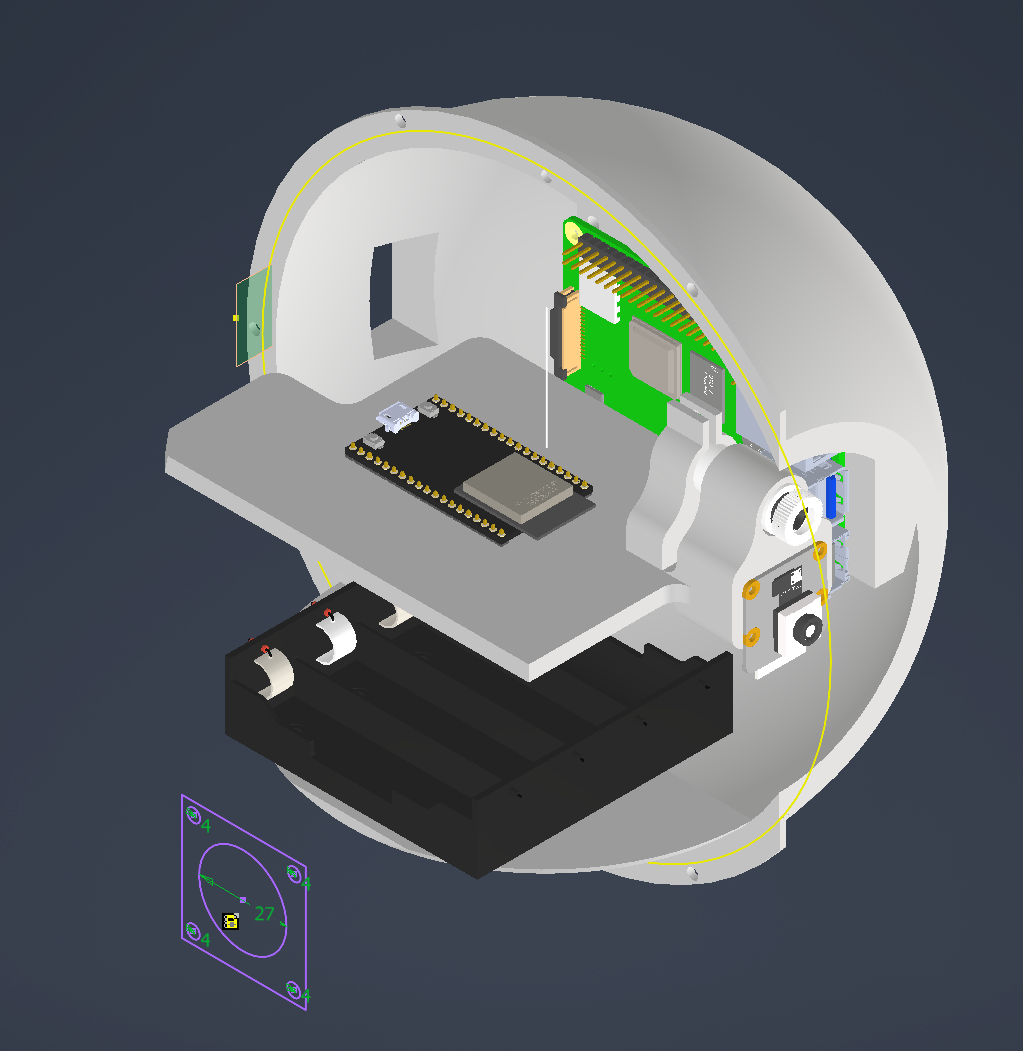
\includegraphics[width=0.7\textwidth]{./Obrazy/Inventor/Komponenty.png}
    \caption{Przekrój głowicy optyczno-elektronicznej prezentujący odwróconą architekturę systemową oraz rozmieszczenie kluczowych komponentów obliczeniowych i zasilania.}
    \label{fig:rozmieszczenie_komponentow}
\end{figure}

Aby zapewnić stabilność tak obciążonej konstrukcji głowicy i zapobiec jej chwianiu podczas nagłych nawrotów, odstąpiono od stosowania cienkich osi obrotu. Zamiast tego zaimplementowano wielkogabarytowe łożysko wieńcowe o średnicy zewnętrznej $140\text{ mm}$ i wewnętrznej $80\text{ mm}$ (widoczne na Rys. \ref{fig:przekladnia_pan}). Jego zastosowanie pozwoliło na maksymalne poszerzenie bazy podparcia dla elementów obrotowych, co skutecznie przenosi momenty wywracające i niweluje luzy promieniowe układu.

Z punktu widzenia kinematyki i procesu montażowego, cały demonstrator został podzielony na trzy współpracujące ze sobą główne moduły mechaniczne:
\begin{itemize}
    \item \textbf{Moduł I: Stacjonarna podstawa bazowa} -- element gwarantujący stabilne osadzenie na podłożu. Ma postać płyty nośnej, w której zintegrowano centralny otwór montażowy pozycjonujący zewnętrzną bieżnię głównego łożyska (Rys. \ref{fig:przekladnia_pan}). Podstawa została wyposażona w nieruchomy wieniec zębaty o zębach daszkowych, z którym współpracuje zębnik układu napędowego osi PAN.
    \item \textbf{Moduł II: Ruchoma platforma nośna} -- element precyzyjnie spasowany z wewnętrzną średnicą łożyska, co zapewnia płynny obrót względem stacjonarnej podstawy (Rys. \ref{fig:jarzmo}). Z jego rdzenia wyprowadzono ramiona pionowe, na których zamontowano silniki krokowe. Silnik osi PAN współpracuje z wieńcem bazy, natomiast silnik osi TILT odpowiada za podnoszenie głowicy optycznej.
    \item \textbf{Moduł III: Głowica optyczno-elektroniczna} -- ruchoma czasza wyposażona we własną zębatkę napędową w płaszczyźnie TILT (Rys. \ref{fig:kopula_calosc}). Stanowi centrum sterowania układem. We wnętrzu zaprojektowano dedykowane punkty montażowe pod obwody drukowane, a w samej obudowie przewidziano precyzyjne otwory przepustowe na okablowanie silników. Moduł uzupełniono o zintegrowany przełącznik bistabilny do natychmiastowego odcinania zasilania aparatury w warunkach testowych.
\end{itemize}

\begin{figure}
    \centering
    \begin{minipage}{0.48\textwidth}
        \centering
        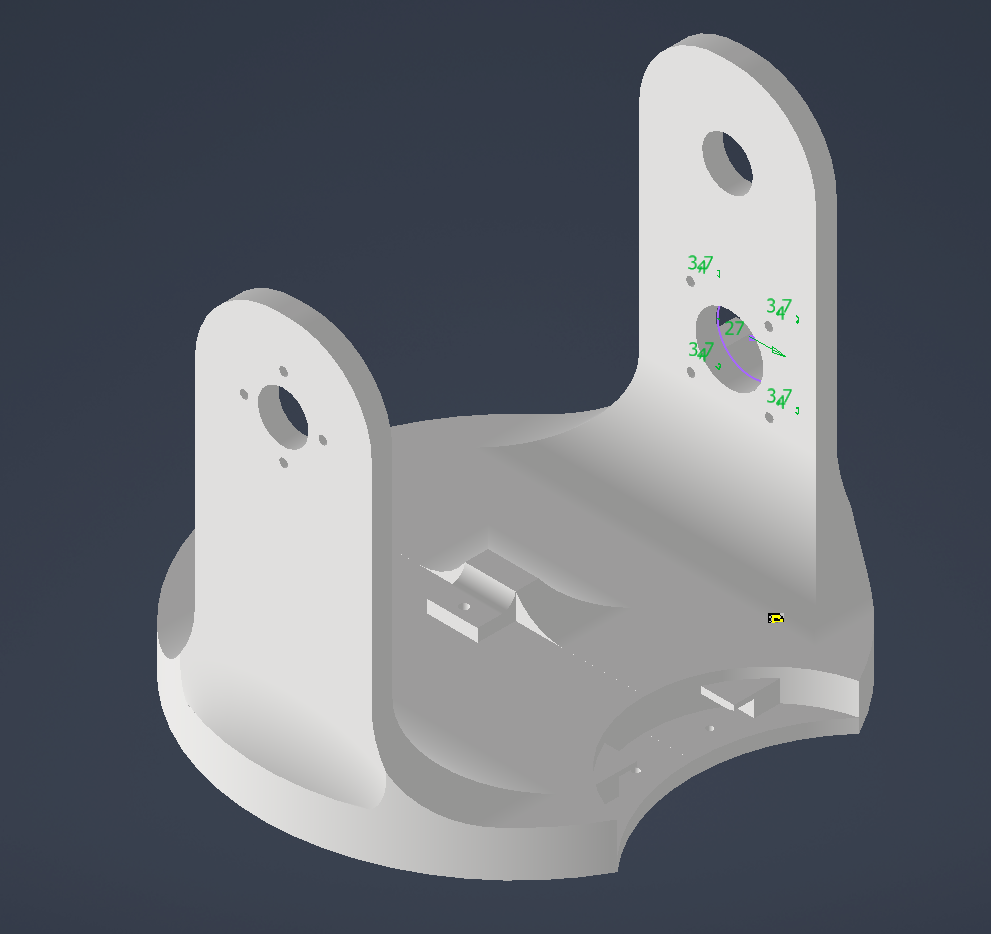
\includegraphics[width=\linewidth]{./Obrazy/Inventor/podstawa gora.png}
        \caption{Model jarzma wsporczego (Moduł II) zapewniającego sztywność skrętną osi poziomej.}
        \label{fig:jarzmo}
    \end{minipage}\hfill
    \begin{minipage}{0.48\textwidth}
        \centering
        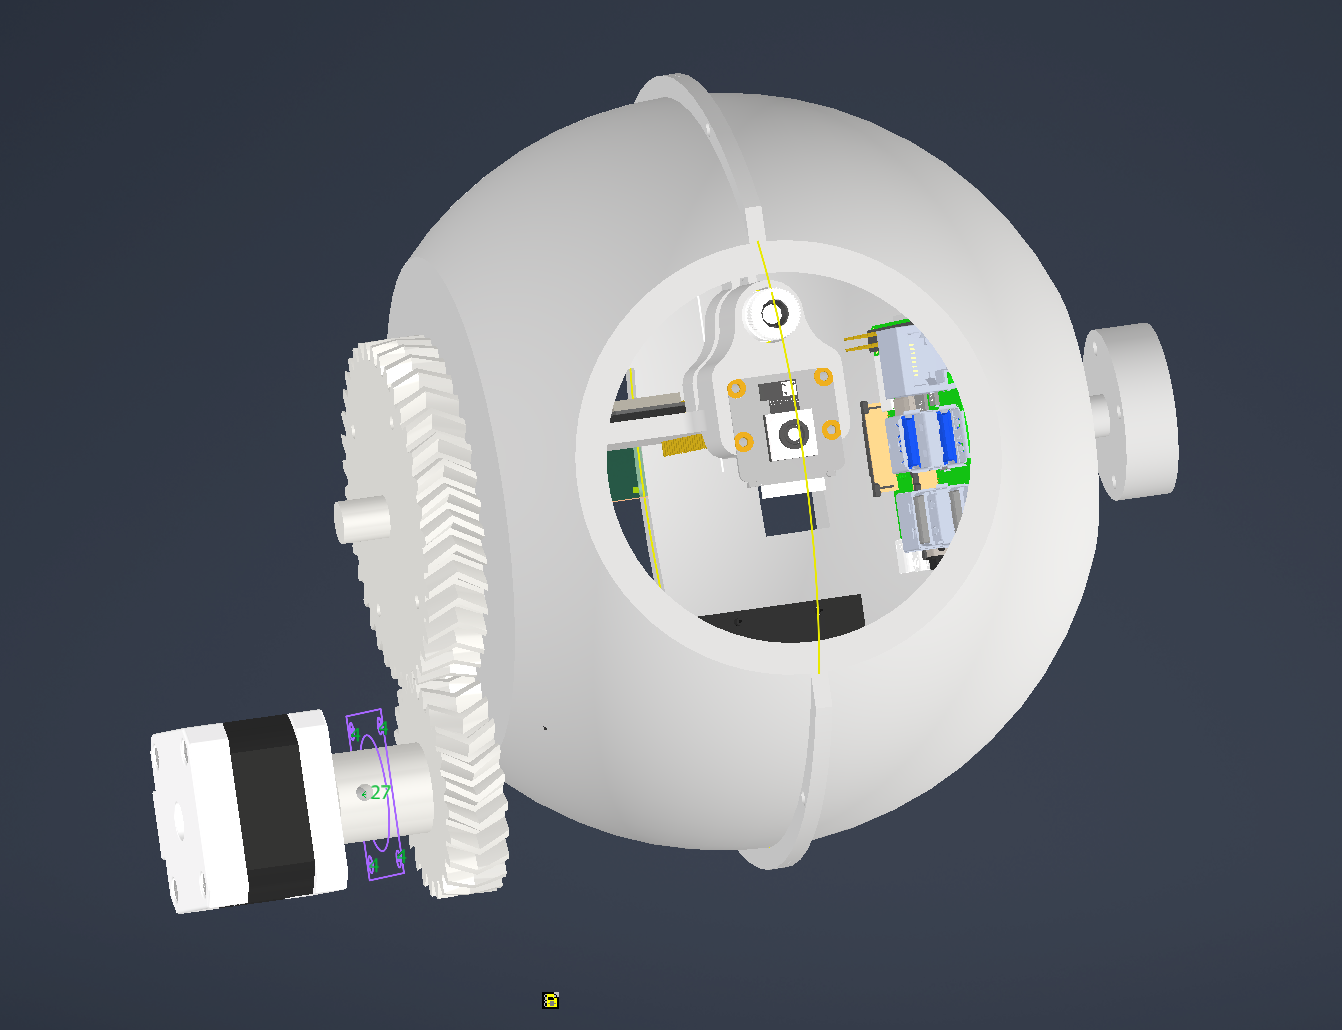
\includegraphics[width=\linewidth]{./Obrazy/Inventor/kopula calosc.png}
        \caption{Zewnętrzny model ruchomej czaszy (Moduł III) ze zintegrowanym wieńcem napędowym osi TILT.}
        \label{fig:kopula_calosc}
    \end{minipage}
\end{figure}

\subsection{Modelowanie przestrzenne i rozkład mas}

Wszystkie elementy mechaniczne demonstratora zostały zamodelowane z wykorzystaniem środowiska projektowego CAD 3D (Rys. \ref{fig:zlozenie_boczne} oraz \ref{fig:zlozenie_tyl}). Cyfrowe odwzorowanie konstrukcji pozwoliło na wczesną detekcję kolizji, odpowiednie tolerowanie otworów pod wały napędowe oraz weryfikację całkowitej przestrzeni roboczej robota.

\begin{figure}[H]
    \centering
    \begin{minipage}{0.48\textwidth}
        \centering
        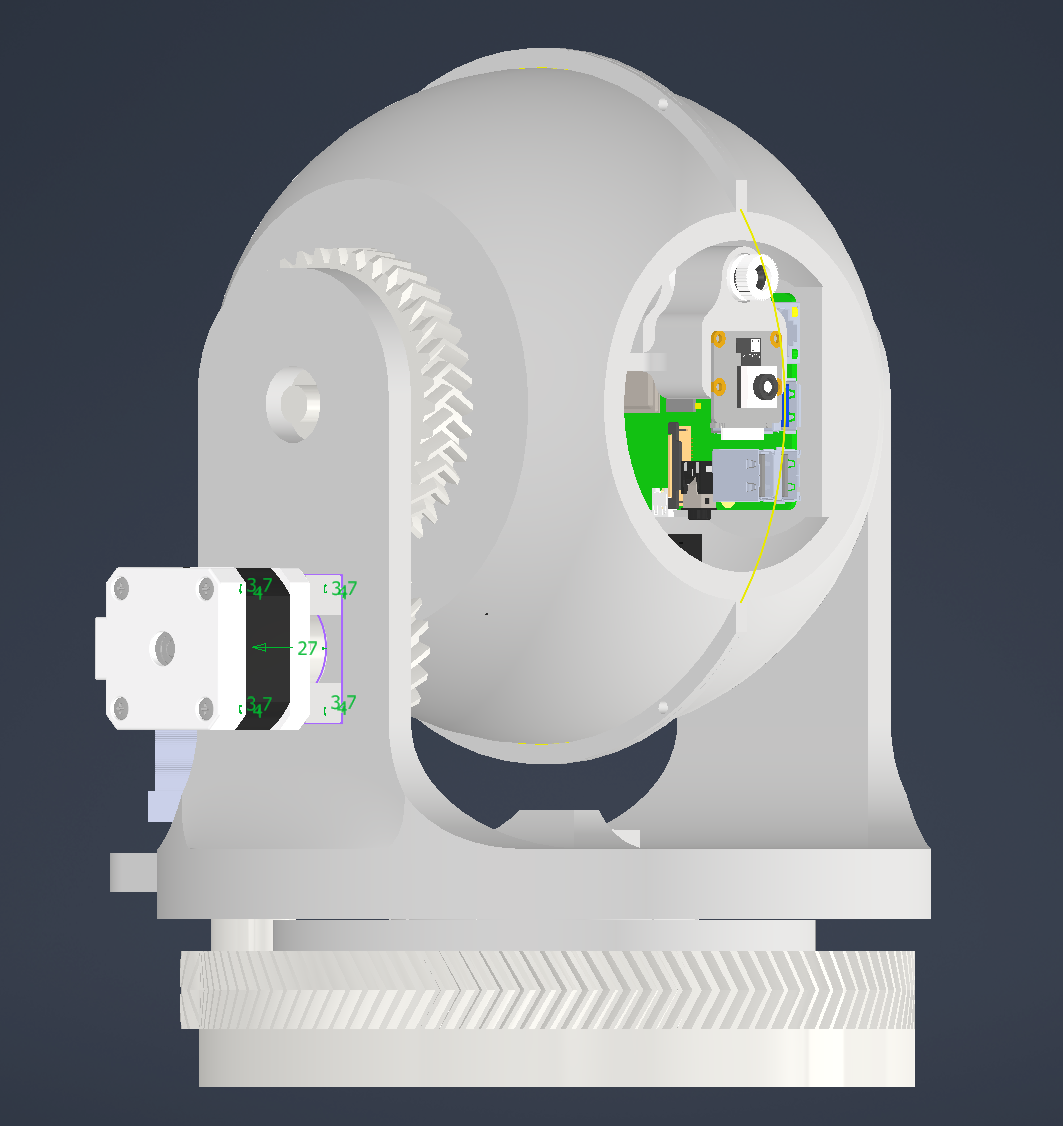
\includegraphics[width=\linewidth]{./Obrazy/Inventor/boczny.png}
        \caption{Widok boczny kompletnego modelu przestrzennego demonstratora układu nadążnego.}
        \label{fig:zlozenie_boczne}
    \end{minipage}\hfill
    \begin{minipage}{0.48\textwidth}
        \centering
        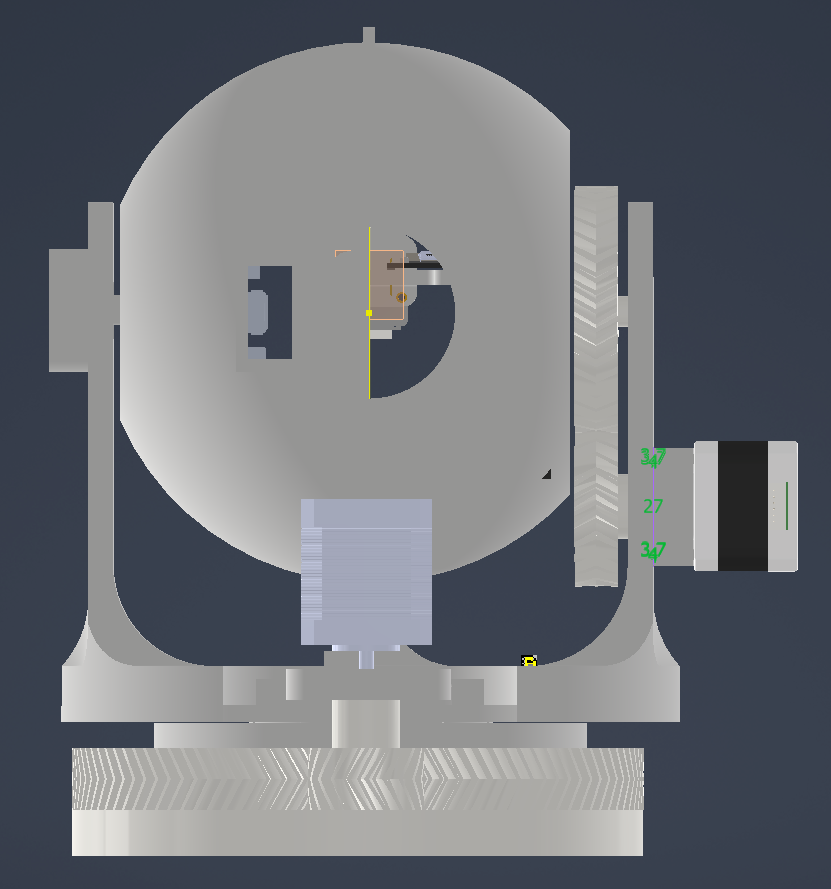
\includegraphics[width=\linewidth]{./Obrazy/Inventor/tył.png}
        \caption{Widok tylny zespołu głowicy, obrazujący umiejscowienie napędów krokowych.}
        \label{fig:zlozenie_tyl}
    \end{minipage}
\end{figure}

Szczególny nacisk podczas projektowania położono na optymalizację rozkładu mas. Zastosowanie dwuramiennego jarzma wsporczego (Moduł II) znacząco zwiększyło sztywność skrętną osi poziomej, zapobiegając ugięciom sprężystym, które dyskwalifikowałyby pomiary dokonywane przez algorytm wizyjny. Ponadto, półki i punkty mocowania wewnętrznej elektroniki oraz kamery z laserem w Module III (Rys. \ref{fig:kopula_przekroj}) dobrano tak, aby środek masy całej kopuły pokrywał się z fizyczną osią obrotu wału TILT. Zbalansowanie układu drastycznie zminimalizowało statyczny moment gnący, co pozwoliło ograniczyć prąd trzymania silników krokowych i zredukować generowanie ciepła.

\begin{figure}[H]
    \centering
    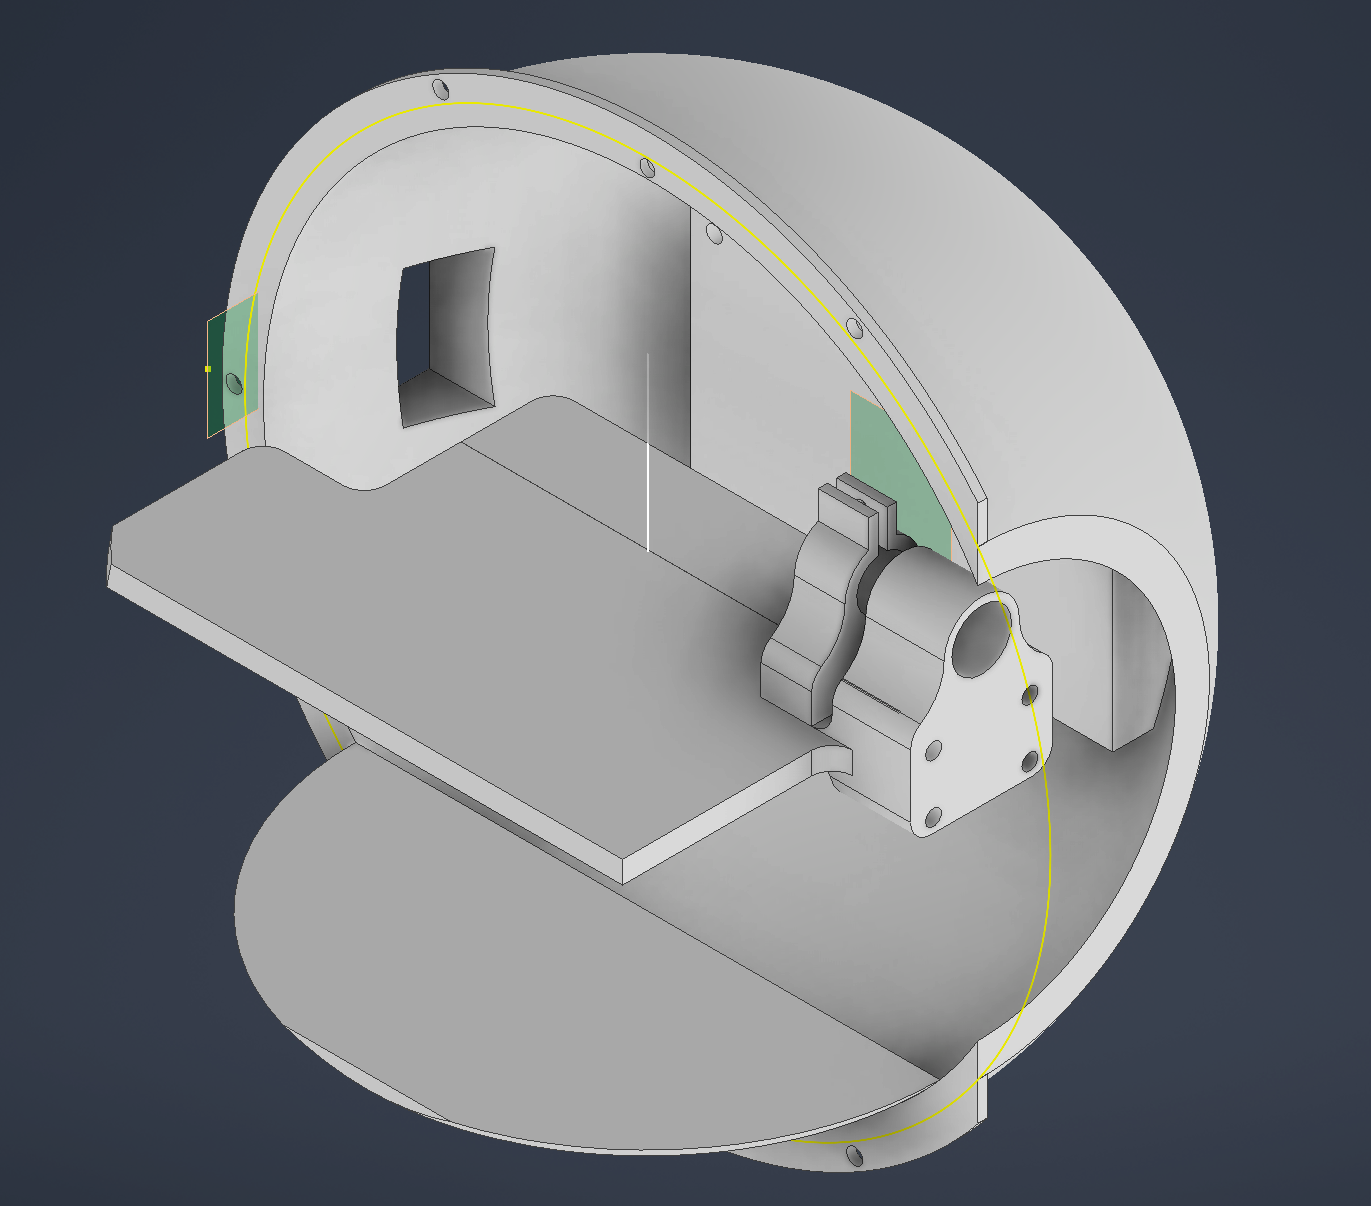
\includegraphics[width=0.6\textwidth]{./Obrazy/Inventor/kopula bok.png}
    \caption{Przekrój czaszy głowicy uwidaczniający wewnętrzne półki montażowe, zaprojektowane w celu optymalnego rozkładu mas i wyważenia układu.}
    \label{fig:kopula_przekroj}
\end{figure}

\subsection{Analiza układu napędowego i przekładni zębatej}

Osiągnięcie odpowiedniej rozdzielczości ruchowej i płynności śledzenia w układach nadążnych wymaga starannego doboru przełożeń redukcyjnych. Zastosowanie tradycyjnych kół zębatych o zębach prostych zostało na wczesnym etapie odrzucone ze względu na nieodłączne zjawisko luzu międzyzębnego. Aby spełnić rygorystyczne wymagania układu celowania, w projekcie wdrożono przekładnie o zębach daszkowych (Rys. \ref{fig:przekladnia_pan}).

\begin{figure}[H]
    \centering
    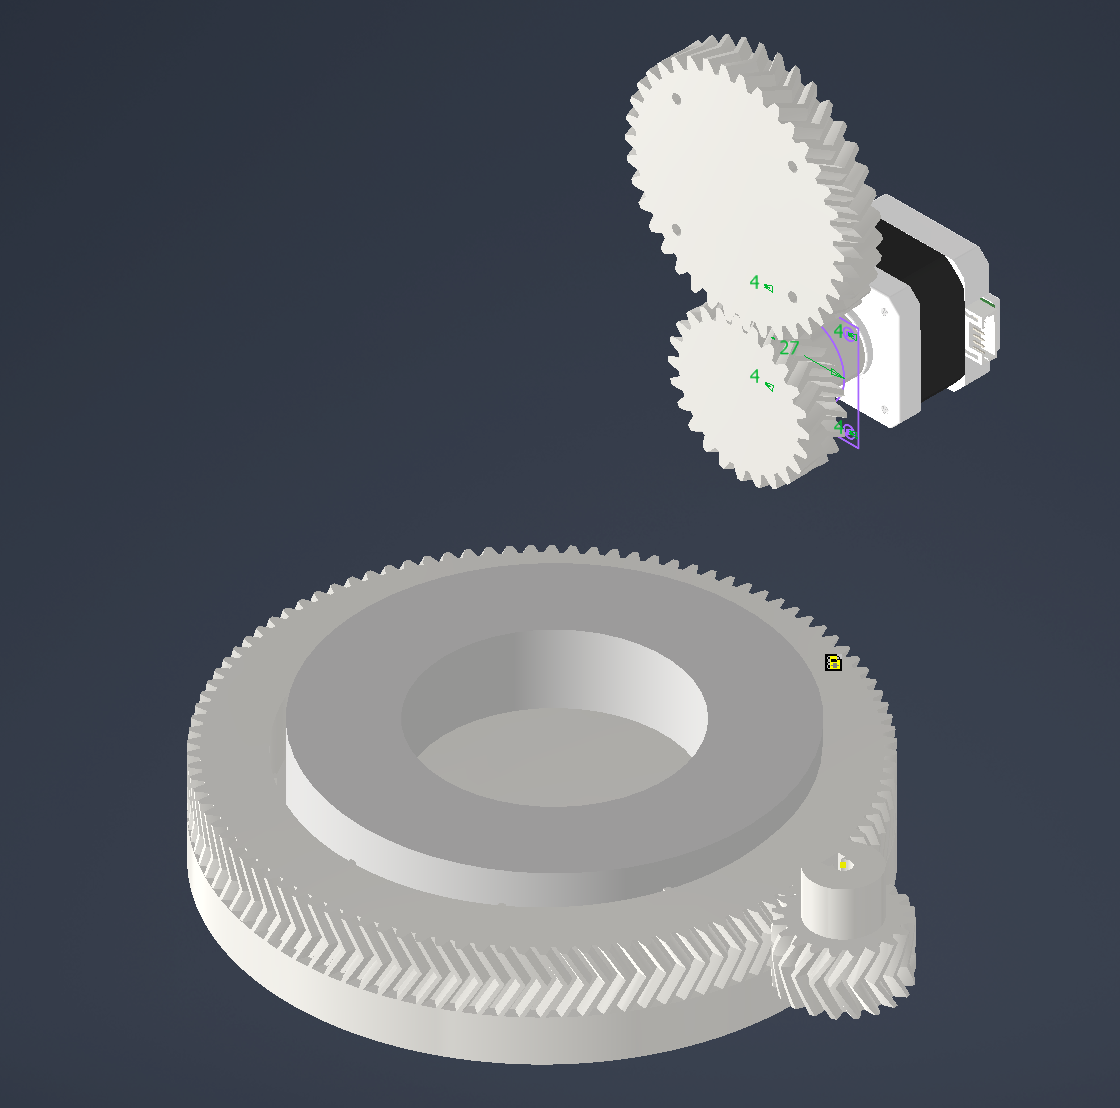
\includegraphics[width=0.6\textwidth]{./Obrazy/Inventor/przekladnia lozysko.png}
    \caption{Model przekładni o zębach daszkowych osi PAN współpracującej ze stacjonarnym wieńcem bazowym.}
    \label{fig:przekladnia_pan}
\end{figure}

Pochylenie linii zęba w dwóch przeciwnych kierunkach powoduje wzajemne znoszenie się sił osiowych, co chroni łożyska silników NEMA przed przedwczesnym zużyciem. Co ważniejsze dla zastosowań robotycznych, zarys daszkowy charakteryzuje się samoosiowaniem współpracujących kół oraz dopuszcza ciaśniejsze spasowanie profilu. Pozwala to na mechaniczną eliminację luzu zwrotnego, zapobiegając szarpaniu i klatkowaniu obrazu przy szybkich zmianach kierunku śledzenia przez mikrokontroler sterujący.

Układ kinematyczny celowo zróżnicowano pod względem redukcji kątowej. Całkowite przełożenie mechaniczne $i$ określa się stosunkiem liczby zębów koła napędzanego $z_2$ do koła napędzającego $z_1$:
\begin{equation}
    i = \frac{z_2}{z_1}
\end{equation}

Dla głównej osi obrotu (PAN), obciążonej znaczną bezwładnością obrotową Modułu II i III, zaprojektowano przekładnię o przełożeniu $i_{PAN} = 5.25$ ($z_1 = \text{20}$, $z_2 = \text{105}$). Wysoka redukcja gwarantuje wymagany moment obrotowy do dynamicznego przyspieszania i hamowania struktury. Z kolei dla osi podnoszenia (TILT), która operuje zbalansowaną masowo głowicą, zastosowano łagodniejsze przełożenie $i_{TILT} = 1.60$ ($z_3 = \text{24}$, $z_4 = \text{38}$), co kompensuje fizyczną prędkość nadążania w pionie.

Zaimplementowane przełożenia bezpośrednio determinują fizyczną rozdzielczość kątową systemu $\Delta\theta$. Dla użytych napędów krokowych o podstawowym skoku wynoszącym $1.8^\circ$, rozdzielczość na wale wyjściowym wyraża się zależnością:
\begin{equation}
    \Delta\theta = \frac{1.8^\circ}{i \cdot \mu}
\end{equation}
gdzie $\mu$ oznacza zaimplementowany mnożnik podziału mikrokroku. Odpowiednie zwiększenie przełożenia redukcyjnego było niezbędne do utworzenia sprzętowego filtru dolnoprzepustowego, zdolnego do wygładzenia mikroskoków silnika i redukcji hałasu mechanicznego wywoływanego przez drobne oscylacje algorytmu śledzącego punkt docelowy.


\section{Architektura sprzętowa i integracja elektroniczna}

Działanie zaprojektowanego układu mechanicznego wymagało implementacji odpowiednio dobranej warstwy elektronicznej. Ze względu na architekturę systemu, obejmującą ciągłą akwizycję strumienia wideo, przetwarzanie obrazu oraz precyzyjne sterowanie napędami, przyjęto rozproszoną architekturę sprzętową. W poniższej sekcji omówiono dobór kluczowych komponentów, strukturę zasilania zapobiegającą propagacji zakłóceń elektromagnetycznych oraz fizyczne interfejsy wymiany danych.

\subsection{Dobór głównych komponentów systemu}

W architekturze systemu wyodrębniono dwa główne poziomy sterowania zlokalizowane bezpośrednio w głowicy: nadrzędny oraz wykonawczy. 

Funkcję pokładowej jednostki nadrzędnej powierzono mikrokomputerowi \textbf{Raspberry Pi 4B} wyposażonemu w 8 GB pamięci RAM. Wybór tej platformy podyktowany był koniecznością uruchomienia bazowego systemu operacyjnego Raspberry Pi OS (opartego na dystrybucji Debian) oraz bezpośredniego wykonywania skryptów sterujących i komunikacyjnych. Duża pojemność pamięci operacyjnej jest istotna dla bezstratnej obsługi strumieni wideo oraz płynnego działania algorytmów detekcji wizyjnej zaimplementowanych z wykorzystaniem biblioteki OpenCV. 

Do akwizycji obrazu wykorzystano dedykowany moduł wizyjny \textbf{[Wpisz model kamery, np. Raspberry Pi Camera Module 2/3]}, który został podłączony do mikrokomputera z wykorzystaniem sprzętowego interfejsu szeregowego MIPI CSI (ang. \textit{Camera Serial Interface}) za pomocą elastycznej taśmy sygnałowej FFC. Zastosowanie tego interfejsu, w przeciwieństwie do kamer podłączanych przez port USB, znacząco zmniejsza obciążenie procesora oraz redukuje opóźnienia w przesyłaniu klatek obrazu do pamięci operacyjnej.

System operacyjny Raspberry Pi OS, jako system z podziałem czasu, nie gwarantuje determinizmu czasowego, co dyskwalifikuje go z bezpośredniego generowania precyzyjnych sygnałów \textit{krok/kierunek} dla sterowników silników. Z tego powodu w warstwie wykonawczej zaimplementowano platformę deweloperską \textbf{ESP32 DevKitC-32E V4} (bazującą na module ESP-WROOM-32E z łącznością Wi-Fi oraz Bluetooth 4.2). Zadaniem mikrokontrolera jest odbiór wyliczonych wartości uchybu oraz sprzętowe, rygorystyczne czasowo taktowanie impulsów sterujących mechaniką.

Do napędu osi PAN i TILT wykorzystano silniki krokowe w standardzie \textbf{NEMA 17}. Charakteryzują się one krokiem podstawowym wynoszącym $1.8^\circ$, co w połączeniu ze sprzętową redukcją przez przekładnie strzałkowe zapewnia wysoką rozdzielczość pozycjonowania. Wysterowanie silników realizowane jest przez zaawansowane sterowniki \textbf{Pololu 36v4 (High-Power Stepper Motor Driver 3730)}. Moduły te tolerują napięcie zasilania do 50 V i prąd ciągły na poziomie 4 A (do 6 A przy zastosowaniu chłodzenia), co daje duży margines bezpieczeństwa termicznego i chroni elektronikę przed uszkodzeniem podczas ciągłego panoramowania z obciążeniem statycznym.

System celowniczy oparto na wymiennych, niskomocowych modułach diod laserowych o mocy $5\text{ mW}$, zasilanych napięciem $5\text{ V}$ i emitujących wiązkę o długości fali $650\text{ nm}$ (pasmo widzialne, kolor czerwony). Zaprojektowany mechanizm mocowania umożliwia szybką wymianę głowic wyposażonych w różne soczewki kolimacyjne (generujące plamkę punktową lub krzyż). Pozwala to na weryfikację precyzji działania algorytmów śledzących punkt padania wiązki.

\subsection{Topologia zasilania i separacja obwodów}

Kluczowym wyzwaniem przy projektowaniu mechatronicznych systemów śledzących jest odizolowanie wrażliwej elektroniki logicznej od zakłóceń elektromagnetycznych (EMI) wprowadzanych przez obciążenia indukcyjne, jakimi są silniki krokowe. Chwilowe spadki napięcia lub przepięcia wsteczne mogłyby prowadzić do niestabilności jednostki nadrzędnej. Aby temu zapobiec, zaimplementowano gwiaździstą topologię dystrybucji energii z jednego, głównego źródła.

Schemat sekcji zasilania (Rys. \ref{fig:schemat_zasilania}) opiera się na pakiecie czterech ogniw litowo-jonowych w układzie 4S (Li-Po 4S), dostarczającym nominalne napięcie na poziomie około 14.8~V (oznaczone jako główna szyna \texttt{+16V\_BATT}). Z głównego węzła zasilającego wyprowadzono trzy niezależne gałęzie zasilania:

\begin{enumerate}
    \item \textbf{Szyna wysokoprądowa napędów (\texttt{+16V\_BATT}):} Napięcie z pakietu ogniw poprowadzono bezpośrednio do złączy zasilających (VIN) sterowniki silników. Zastosowanie relatywnie wysokiego napięcia wejściowego znacząco poprawia dynamikę narastania prądu w cewkach, co pozwala na osiąganie większych prędkości obrotowych osi PAN i TILT bez utraty momentu trzymającego.
    \item \textbf{Gałąź logiczna jednostki nadrzędnej (\texttt{+5V\_RPi}):} Do zasilania mikrokomputera wykorzystano impulsową przetwornicę obniżającą (step-down) Pololu D24V50F5, charakteryzującą się wysoką wydajnością prądową rzędu 5~A. Na wejściu przetwornicy zastosowano kondensator filtrujący o pojemności 470~$\mu$F, którego zadaniem jest tłumienie impulsów napięciowych (tzw. \textit{LC voltage spikes}) powstających podczas włączania zasilania.
    \item \textbf{Gałąź peryferyjna efektora (\texttt{+5V\_LASER}):} Moduł lasera zasilany jest z dedykowanej, separowanej przetwornicy obniżającej napięcie do 5~V. Takie odseparowanie gwarantuje, że wahania poboru prądu przez diodę laserową nie wpłyną na stabilność pracy jednostek obliczeniowych.
\end{enumerate}

Wszystkie gałęzie zasilające posiadają wspólną płaszczyznę masy (\texttt{GND}), co jest warunkiem koniecznym do poprawnej transmisji sygnałów cyfrowych pomiędzy modułami.

\begin{figure}
    \centering
    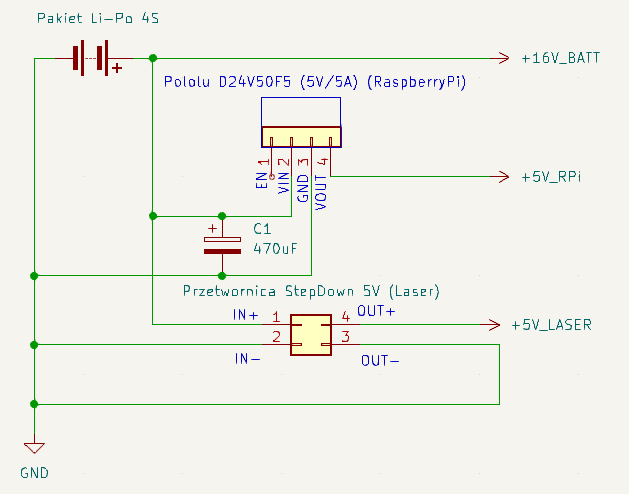
\includegraphics[width=0.7\textwidth]{./Obrazy/Schemat elektryczny/Zasilanie.png} % Podmień na właściwą nazwę pliku
    \caption{Schemat ideowy układu zasilania uwzględniający pakiet ogniw 4S oraz przetwornice napięcia.}
    \label{fig:schemat_zasilania}
\end{figure}

\subsection{Jednostka nadrzędna, interfejsy i komunikacja}

Za zarządzanie systemem, przetwarzanie wizyjne i wyliczanie uchybu śledzenia odpowiada mikrokomputer Raspberry Pi 4 (Rys. \ref{fig:schemat_mozgu}). Do sprzętowej akwizycji obrazu wykorzystano dedykowaną kamerę podłączoną za pomocą elastycznej taśmy FFC do portu MIPI CSI-2. Rozwiązanie to pozwala na bezpośredni dostęp do strumienia wideo z pominięciem obciążających procesor magistrali USB, minimalizując opóźnienia transportowe w układzie zamkniętej pętli sprzężenia zwrotnego.

Z uwagi na brak determinizmu czasowego w systemie operacyjnym Raspberry Pi OS, precyzyjne taktowanie silników krokowych powierzono mikrokontrolerowi wykonawczemu ESP32-DevKitC-32E V4. Połączenie pomiędzy jednostkami zrealizowano za pomocą przewodu USB, który pełni podwójną funkcję:
\begin{itemize}
    \item \textbf{Zasilającą:} Dostarcza napięcie 5~V bezpośrednio z portu Raspberry Pi do stabilizatora napięcia na płytce ESP32.
    \item \textbf{Komunikacyjną:} Umożliwia asynchroniczną transmisję szeregową (\textit{UART over USB}) danych o docelowych pozycjach kątowych obu osi, przy prędkości 115200~bps.
\end{itemize}

\begin{figure}
    \centering
    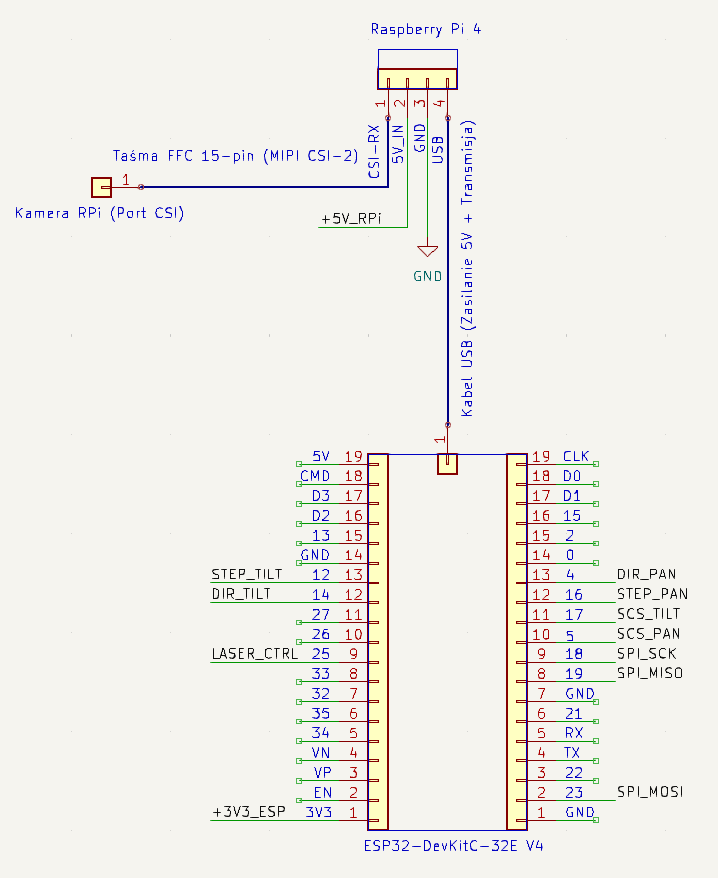
\includegraphics[width=0.7\textwidth]{./Obrazy/Schemat elektryczny/Rpi_ESP.png} % Podmień na właściwą nazwę pliku
    \caption{Architektura połączeń jednostki nadrzędnej (Raspberry Pi) z układem wykonawczym (ESP32).}
    \label{fig:schemat_mozgu}
\end{figure}

\subsection{Układ wykonawczy napędów i magistrala SPI}

Za pozycjonowanie mechanizmu odpowiadają silniki krokowe NEMA 17, sterowane przez zaawansowane moduły Pololu 36v4 (Rys. \ref{fig:schemat_sterownikow}). Umożliwiają one precyzyjne mikrokrokowanie oraz programową kontrolę prądu cewek.

Integracja sterowników z płytą bazową i mikrokontrolerem ESP32 wymagała poprowadzenia następujących sygnałów sterujących:
\begin{itemize}
    \item \textbf{Zasilanie logiki:} Wykorzystano zintegrowany stabilizator LDO mikrokontrolera ESP32, doprowadzając napięcie referencyjne 3.3~V (\texttt{+3V3\_ESP}) do wejść \texttt{IOREF}, \texttt{SLEEP} oraz \texttt{RESET} obu sterowników.
    \item \textbf{Konfiguracja sprzętowa (SPI):} Magistrala SPI (\texttt{SPI\_MOSI}, \texttt{SPI\_MISO}, \texttt{SPI\_SCK}) jest współdzielona dla obu modułów. Indywidualne adresowanie podczas inicjalizacji odbywa się za pomocą linii wyboru układu: \texttt{SCS\_PAN} oraz \texttt{SCS\_TILT}.
    \item \textbf{Sygnały krok/kierunek:} Fizyczny ruch wymuszany jest poprzez sygnały logiczne na liniach \texttt{STEP\_PAN} / \texttt{DIR\_PAN} oraz \texttt{STEP\_TILT} / \texttt{DIR\_TILT}, obsługiwanych sprzętowo przez timery ESP32.
\end{itemize}

\begin{figure}
    \centering
    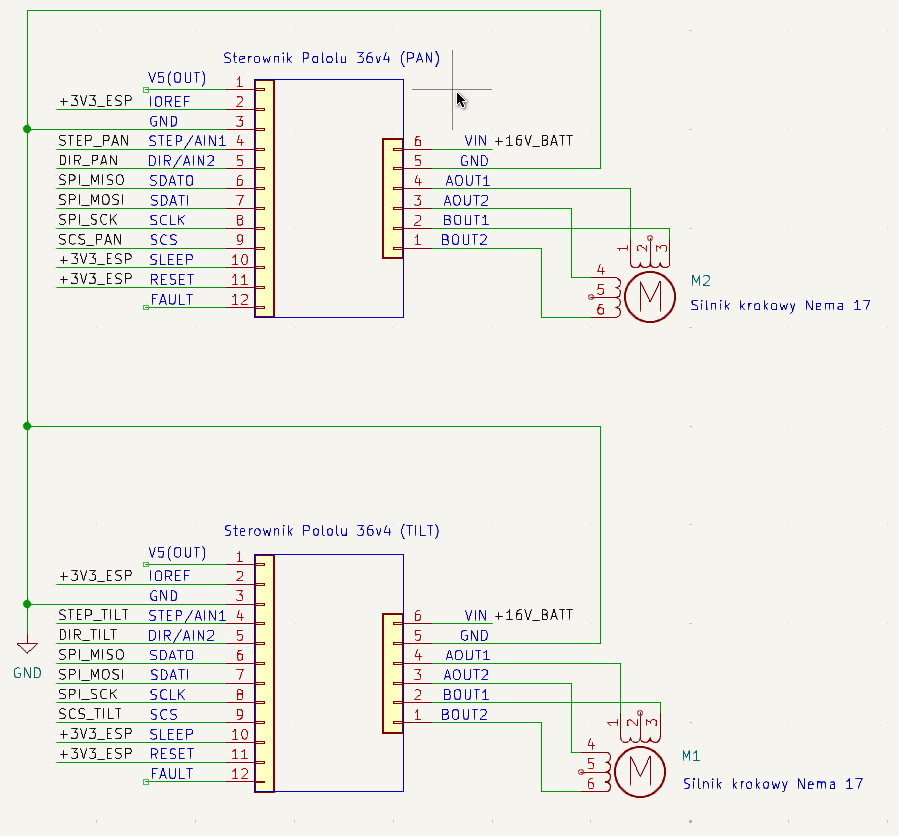
\includegraphics[width=0.8\textwidth]{./Obrazy/Schemat elektryczny/Silniki.png} % Podmień na właściwą nazwę pliku
    \caption{Układ wykonawczy napędów PAN/TILT z wykorzystaniem sterowników Pololu 36v4 i komunikacji SPI.}
    \label{fig:schemat_sterownikow}
\end{figure}

\subsection{Układ kluczujący efektora (Laser)}

System wyposażono w 5~mW moduł diody laserowej pełniący rolę wskaźnika punktu śledzenia. Piny wyjściowe GPIO mikrokontrolera ESP32 nie dysponują wydajnością prądową pozwalającą na bezpośrednie zasilenie emitera 5~V, dlatego na płycie zaimplementowano sprzętowy układ dopasowujący (Rys. \ref{fig:schemat_lasera}).

Do kluczowania obwodu wykorzystano tranzystor bipolarny NPN. Sygnał cyfrowy (\texttt{LASER\_CTRL}) z pinu 25 mikrokontrolera doprowadzono do bazy tranzystora poprzez rezystor ograniczający prąd o wartości 1~k$\Omega$. Zasilanie główne diody poprowadzono z niezależnej linii \texttt{+5V\_LASER}, a obwód zamyka się do masy poprzez złącze kolektor-emiter tranzystora. Przełącznik typu \textit{low-side} gwarantuje separację portów procesora od zasilania efektora, umożliwiając niezawodne, programowe sterowanie wiązką.

\begin{figure}
    \centering
    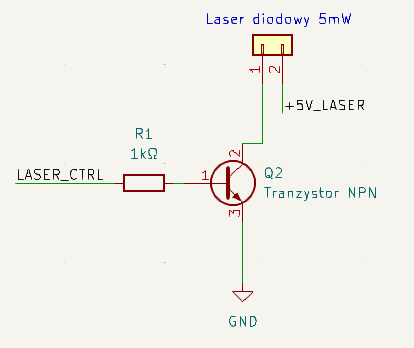
\includegraphics[width=0.5\textwidth]{./Obrazy/Schemat elektryczny/Laser.png} % Podmień na właściwą nazwę pliku
    \caption{Schemat elektryczny układu kluczującego moduł lasera za pomocą tranzystora NPN.}
    \label{fig:schemat_lasera}
\end{figure}
%\begin{figure}
%\centering
%
\includegraphics[width=0.5\textwidth]{./politechnika_sl_logo_bw_pion_pl.pdf}
%\caption{Podpis rysunku zawsze pod rysunkiem.}
%\label{fig:etykieta-rysunku}
%\end{figure}

% \begin{figure}[H]
%     \centering
%     % \includegraphics[width=0.9\textwidth]{sciezka_do_schematu_elektrycznego.png}
%     \caption{Schemat elektryczny układu sterowania, przedstawiający interfejsy komunikacyjne oraz kluczowanie diody laserowej.}
%     \label{fig:schemat_elektroniki}
% \end{figure}

\chapter{Architektura oprogramowania i symulacja systemu}

\section{Środowisko uruchomieniowe}
Złożoność współczesnych systemów robotycznych wymaga zastosowania wydajnego i niezawodnego środowiska programistycznego, które gwarantuje determinizm działania oraz powtarzalność wyników. Główną platformą deweloperską oraz stacją operatorską w opisywanym projekcie jest komputer przenośny wyposażony w procesor \textbf{[Wpisz model procesora, np. Intel Core i7-12700H]}, \textbf{[Wpisz ilość] GB} pamięci operacyjnej RAM oraz dedykowany układ graficzny \textbf{[Wpisz model karty, np. NVIDIA GeForce RTX 3060]}. Systemem operacyjnym hosta jest dystrybucja GNU/Linux Ubuntu w wersji 22.04 LTS (Jammy Jellyfish). Wybór ten podyktowany był natywnym wsparciem dla wybranych dystrybucji oprogramowania robotycznego oraz wysoką stabilnością jądra systemu. Edycję kodu źródłowego, zarządzanie repozytorium kontroli wersji (Git) oraz analizę logów realizowano w zintegrowanym środowisku programistycznym (IDE) Visual Studio Code.

W celu odizolowania zależności projektowych od głównego systemu operacyjnego oraz zapewnienia pełnej przenośności kodu, całe środowisko uruchomieniowe zostało zaimplementowane w architekturze kontenerowej z wykorzystaniem platformy Docker. Konteneryzacja eliminuje powszechny problem konfliktów wersji bibliotek programistycznych. Środowisko definiowane jest poprzez plik konfiguracyjny \texttt{Dockerfile}, który bazuje na oficjalnym, stabilnym obrazie \texttt{osrf/ros:humble-desktop}:

\begin{lstlisting}[language=bash, basicstyle=\ttfamily\scriptsize, frame=single, breaklines=true]
FROM osrf/ros:humble-desktop

RUN apt-get update && apt-get install -y \
    ros-humble-cv-bridge \
    python3-opencv \
    ros-humble-foxglove-bridge \
    ros-humble-rviz2 \
    ros-humble-rviz-common \
    ros-humble-rviz-default-plugins \
    ros-humble-xacro \
    ros-humble-ros-gz \
    python3-pyqt5 \
    python3-numpy \
    ros-humble-image-transport \
    ros-humble-image-transport-plugins \
    ros-humble-rqt \
    ros-humble-rqt-common-plugins \
    ros-humble-rqt-image-view \
    python3-pip \
    python3-serial \
    nano \
    alsa-utils \
    mpg123 \
    gstreamer1.0-plugins-ugly \
    libsdl2-mixer-2.0-0 \
    && rm -rf /var/lib/apt/lists/*

RUN pip3 install pyzmq pygame pandas matplotlib "numpy<2"
\end{lstlisting}

Powyższa konfiguracja instaluje wszystkie pakiety niezbędne do pracy systemu. Obejmują one mosty komunikacyjne dla wizji maszynowej (\texttt{cv-bridge}, \texttt{python3-opencv}), środowiska symulacyjne i wizualizacyjne (\texttt{ros-gz}, \texttt{foxglove-bridge}, \texttt{rviz2}), narzędzia do transformacji modeli (\texttt{xacro}) oraz biblioteki interfejsów graficznych i przetwarzania danych dla języka Python (\texttt{pyqt5}, \texttt{numpy}, \texttt{pandas}, \texttt{matplotlib}). Dodatkowo zintegrowano pakiety obsługi multimediów (\texttt{alsa-utils}, \texttt{pygame}) konieczne do generowania dźwiękowych sygnałów ostrzegawczych w aplikacji GUI.

Uruchomienie tak spreparowanego środowiska następuje poprzez zbudowanie obrazu, a następnie wywołanie kontenera z odpowiednimi flagami przekierowującymi serwer wyświetlania X11 (dla obsługi okien GUI) oraz interfejsy audio i sieciowe:

\begin{lstlisting}[language=bash, basicstyle=\ttfamily\scriptsize, frame=single, breaklines=true]

docker build -t master_pan_tilt_env .

docker run -it --rm --net=host --device /dev/snd -e DISPLAY=$DISPLAY -v /tmp/.X11-unix:/tmp/.X11-unix -v ~/Robotyka/Master-Thesis/Color_detection_ros_Ubuntu:/workspace -w /workspace master_pan_tilt_env bash
\end{lstlisting}
Po wykonaniu powyższej komendy użytkownik uzyskuje dostęp do powłoki \texttt{bash} wewnątrz hermetycznego środowiska z zainstalowanym i skonfigurowanym frameworkiem ROS 2 (Robot Operating System 2) w wersji Humble Hawksbill. Zastosowanie środowiska ROS 2 w stacji operatorskiej, pomimo implementacji głównych algorytmów na Raspberry Pi w trybie skryptowym, było konieczne z uwagi na potrzebę przeprowadzenia zaawansowanych symulacji fizycznych, łatwość modelowania kinematyki (TF2) oraz dostęp do potężnych narzędzi analitycznych, które w przyszłości pozwolą na łatwą rozbudowę układu o kolejne węzły decyzyjne.

\section{Implementacja w systemie ROS2}
\subsection{Architektura oprogramowania}
Struktura plików w przestrzeni roboczej ROS 2 została zorganizowana w sposób modułowy, zgodnie z wytycznymi narzędzia budującego \texttt{colcon}. Głównym pakietem integrującym zarówno aspekty wizualizacyjne, jak i symulacyjne jest \texttt{pan\_tilt\_description}. Drzewo katalogów prezentuje się następująco:

\begin{lstlisting}[basicstyle=\ttfamily\scriptsize, frame=single]
src/pan_tilt_description/
|-- CMakeLists.txt
|-- package.xml
|-- gui/
|   `-- turret_gui.py
|   `-- laser.mp3
|-- launch/
|   `-- sim_launch.py
|   `-- visualize_launch.py
|-- meshes/
|   `-- base_link.stl
|   `-- pan_link.stl
|   `-- tilt_link.stl
|-- rviz/
|   `-- config.rviz
|-- urdf/
|   `-- turret.urdf.xacro
`-- worlds/
    `-- tracking_world.sdf
\end{lstlisting}

Sercem warstwy interakcji z robotem fizycznym jest skrypt \texttt{turret\_gui.py} zlokalizowany w katalogu \texttt{gui/}. Aplikacja ta stanowi scentralizowane centrum dowodzenia, które pomija abstrakcję warstwy ROS 2 na rzecz bezpośredniej, niskolatencyjnej komunikacji asynchronicznej (ZeroMQ) z fizycznym mikrokontrolerem Raspberry Pi. Katalog \texttt{urdf/} oraz \texttt{meshes/} stanowią fundament dla modułu symulacyjnego, przechowując odpowiednio matematyczny opis łańcucha kinematycznego oraz rzeczywiste pliki przestrzenne STL wyeksportowane ze środowiska CAD. Katalog \texttt{launch/} zawiera skrypty rozruchowe w języku Python, które automatyzują proces podnoszenia wielu węzłów symulacyjnych, wizualizacyjnych oraz mostów komunikacyjnych jednocześnie.

\section{Model symulacyjny w Gazebo}
Przed wdrożeniem i testowaniem algorytmów sterowania na rzeczywistym obiekcie fizycznym, przeprowadzono proces modelowania i weryfikacji w wirtualnym środowisku symulacyjnym. Pozwala to na zminimalizowanie ryzyka uszkodzenia sprzętu w wyniku niestabilności algorytmów regulacji (np. zjawiska rezonansu lub błędu w ograniczeniach przestrzennych).

\subsection{Definicja kinematyki - URDF i modele STL}
Model efektora został przeniesiony do przestrzeni wirtualnej przy użyciu formatu URDF (Unified Robot Description Format) sprzężonego z językiem makr XACRO. Struktura ta definiuje robota jako graf skierowany, w którym węzłami są fizyczne bryły, a krawędziami połączenia kinematyczne. W dołączonym pliku \texttt{turret.urdf.xacro} zdefiniowano trzy główne człony: nieruchomą podstawę (\texttt{base\_link}), obrotowe ramię poziome (\texttt{pan\_link}) oraz ruchomą głowicę wertykalną (\texttt{tilt\_link}). Pomiędzy nimi zdefiniowano połączenia typu \texttt{revolute}, narzucając im programowe limity wychyleń zgodne z rzeczywistą mechaniką.

W celu wiernego odwzorowania gabarytów i rozkładu mas, jako geometrie kolizyjne (\texttt{<collision>}) oraz wizualne (\texttt{<visual>}) wczytano przestrzenne pliki STL z katalogu \texttt{meshes/}. Modele te zostały uprzednio wyeksportowane ze środowiska Autodesk Inventor.

\subsection{Wirtualna sensoryka i silnik fizyki}
Do przeprowadzenia symulacji zachowania układu wykorzystano zaawansowane środowisko Gazebo (dawniej Ignition Gazebo)[cite: 9]. W obrębie definicji URDF umieszczono dedykowane wtyczki dla silnika symulacyjnego, które pełnią rolę cyfrowych bliźniaków fizycznych komponentów robota. Najistotniejszą z nich jest wirtualna kamera, zdefiniowana na końcu łańcucha kinematycznego (na członie \texttt{camera\_link})[cite: 5, 6]. Sensor ten generuje syntetyczny strumień wideo oraz dane macierzowe, zachowując przy tym parametry fizycznego układu optycznego[cite: 6]. Kąt widzenia (FOV) ustalono na poziomie $1.396$ radiana, rozdzielczość na $640 \times 480$ pikseli (format kodowania przestrzeni barw RGB888), natomiast częstotliwość odświeżania na 30 Hz[cite: 6, 7]. Poniższy fragment kodu z pliku definiującego kinematykę wieżyczki prezentuje wdrożenie tego sensora oraz konfigurację tematu sieciowego dla systemu ROS 2[cite: 6, 7]:

\begin{lstlisting}[language=XML, basicstyle=\ttfamily\small, frame=single, breaklines=true]
  <gazebo reference="camera_link">
    <sensor name="main_camera" type="camera">
      <camera>
        <horizontal_fov>1.396</horizontal_fov>
        <image>
          <width>640</width>
          <height>480</height>
          <format>R8G8B8</format>
        </image>
        <clip>
          <near>0.02</near>
          <far>100.0</far>
        </clip>
      </camera>
      <always_on>1</always_on>
      <update_rate>30</update_rate>
      <visualize>true</visualize>
      <topic>camera/image_raw</topic>
    </sensor>
  </gazebo>
\end{lstlisting}

Za wprawianie symulowanych członów konstrukcyjnych w ruch odpowiada wtyczka kontrolera trajektorii stawów (ang. Joint Position Controller)[cite: 8]. Narzędzie to zastępuje fizyczne silniki krokowe NEMA 17 i układy sterujące Pololu, realizując przemieszczenia bezpośrednio w silniku fizyki przy użyciu wewnętrznego regulatora PID[cite: 8]. Otrzymuje ono żądany kąt za pomocą dedykowanego tematu ROS i aplikuje odpowiedni moment siły na wirtualny wał[cite: 8]. Przykładowa implementacja tego węzła wykonawczego dla osi wertykalnej (TILT) została zdefiniowana następująco[cite: 8]:

\begin{lstlisting}[language=XML, basicstyle=\ttfamily\small, frame=single, breaklines=true]
  <gazebo>
    <plugin filename="libignition-gazebo-joint-position-controller-system.so"
            name="ignition::gazebo::systems::JointPositionController">
      <joint_name>tilt_joint</joint_name>
      <topic>model/pan_tilt_turret/joint/tilt_joint/cmd_pos</topic>
      <p_gain>5.0</p_gain>
      <i_gain>0.1</i_gain>
      <d_gain>0.5</d_gain>
    </plugin>
  </gazebo>
\end{lstlisting}

Integralną częścią całego środowiska symulacyjnego jest zamknięty wirtualny świat, w którym wieżyczka przeprowadza proces śledzenia. Środowisko to zostało zdefiniowane w pliku \texttt{target\_world.sdf} i korzysta z silnika fizyki ODE (ang. Open Dynamics Engine)[cite: 9]. Oprócz podstawowych uwarunkowań takich jak grawitacja, oświetlenie kierunkowe czy płaszczyzna podłoża, wykreowano w nim dynamiczny obiekt referencyjny, nazywany kulką treningową[cite: 9, 10, 11, 12]. Obiekt ten powołano jako encję typu \texttt{actor}, co pozwala na jego przemieszczanie się w sposób deterministyczny, z pominięciem obciążeń wynikających z przeliczania rozbudowanej fizyki zderzeń[cite: 12]. 

Kulka o promieniu $0.15$ m i intensywnie czerwonym kolorze porusza się w pętli zamkniętej po zdefiniowanych punktach orientacyjnych (ang. waypoints), rysując w przestrzeni trajektorię o kształcie kwadratu[cite: 12, 13]. Węzły trasy obejmują jednoczesne przemieszczenia w osiach X, Y oraz Z (np. od wysokości $0.5$ m do $1.2$ m), zmuszając oba stawy wieżyczki (PAN i TILT) do ciągłej, zsynchronizowanej pracy[cite: 13]. Odpowiedzialny za ten ruch fragment kodu przedstawiono poniżej[cite: 12, 13]:

\begin{lstlisting}[language=XML, basicstyle=\ttfamily\small, frame=single, breaklines=true]
    <actor name="target_ball">
      <link name="link">
        <visual name="visual">
          <geometry><sphere><radius>0.15</radius></sphere></geometry>
          <material>
            <ambient>1 0 0 1</ambient>
            <diffuse>1 0 0 1</diffuse>
          </material>
        </visual>
      </link>
      <script>
        <loop>true</loop>
        <delay_start>0.0</delay_start>
        <auto_start>true</auto_start>
        <trajectory id="0" type="square">
           <waypoint><time>0.0</time><pose> 1.5 3.0 0.5 0 0 0</pose></waypoint>
           <waypoint><time>2.0</time><pose>-1.5 3.0 0.5 0 0 0</pose></waypoint>
           <waypoint><time>4.0</time><pose>-1.5 3.0 1.2 0 0 0</pose></waypoint>
           <waypoint><time>6.0</time><pose> 1.5 3.0 1.2 0 0 0</pose></waypoint>
           <waypoint><time>8.0</time><pose> 1.5 3.0 0.5 0 0 0</pose></waypoint>
        </trajectory>
      </script>
    </actor>
\end{lstlisting}

Tak przygotowane i w pełni zautomatyzowane środowisko pozwala algorytmom analitycznym powtarzalnie uczyć się reakcji na zadany bodziec ruchowy, co jest bezpośrednio wykorzystywane w procesie samostrojenia (auto-tuningu) optymalnych nastaw regulatora PID.

\subsection{Wizualizacja w środowisku Foxglove}
Ze względu na konieczność nowoczesnego i wydajnego obrazowania przepływu danych telemetrycznych, klasyczne narzędzie RViz2 zostało w wielu aspektach zastąpione przez platformę Foxglove Studio. Dzięki instalacji pakietu \texttt{ros-humble-foxglove-bridge}, symulowany strumień wideo z Gazebo, a także bieżące parametry odchylenia kątowego poszczególnych stawów (TF) są strumieniowane na zewnątrz kontenera przez protokół WebSocket. Foxglove pozwala na konstruowanie wysoce responsywnych pulpitów analitycznych, w których zintegrowano widok przestrzenny 3D z nałożonymi wektorami sił oraz macierze obrazu RGB.

% \begin{figure}[H]
%     \centering
%     % \includegraphics[width=0.9\textwidth]{images/gazebo_simulation.png}
%     \vspace{6cm} % Puste miejsce na Twoj obrazek
%     \caption{Model symulacyjny wieżyczki w środowisku Gazebo śledzący wirtualną, poruszającą się sferę.}
%     \label{fig:gazebo_sim}
% \end{form}

% \begin{figure}[H]
%     \centering
%     % \includegraphics[width=0.9\textwidth]{images/foxglove_dashboard.png}
%     \vspace{6cm} % Puste miejsce na Twoj obrazek
%     \caption{Pulpit analityczny Foxglove Studio prezentujący drzewo kinematyczne oraz wirtualny strumień wideo z kamery efektora.}
%     \label{fig:foxglove_dash}
% \end{figure}

\subsection{Algorytm samouczenia i optymalizacji nastaw (Auto-tuning)}
Kluczowym elementem badawczym opracowanym w środowisku symulacyjnym był algorytm poszukujący optymalnych nastaw regulatora PID. Zamiast manualnie dobierać wzmocnienia na obiekcie fizycznym, w wirtualnym świecie (plik \texttt{tracking\_world.sdf}) umieszczono sferyczny obiekt o zadanym kolorze, podlegający ciągłemu ruchowi harmonicznemu.

Zaimplementowany węzeł analityczny w ROS 2 cyklicznie uruchamia symulację śledzenia, perturbując parametry wektora nastaw $K = [K_p, K_i, K_d]$. Algorytm ten na podstawie syntetycznego obrazu oblicza w czasie rzeczywistym uchyb średniokwadratowy (RMSE) położenia pikseli obiektu od centrum kamery. Po każdej iteracji wirtualnego ruchu, system automatycznie koryguje nastawy w kierunku gradientu spadku błędu, zachowując stabilność pętli sprzężenia zwrotnego. Po konwergencji algorytmu i ustaleniu optymalnych parametrów w sterylnym środowisku wirtualnym, wyliczone nastawy są walidowane i przenoszone jako wartości startowe do interfejsu graficznego \texttt{turret\_gui.py} sterującego fizycznym obiektem.

\chapter{Algorytmy wizyjne i układy sterowania}

\section{Implementacja algorytmów detekcji i śledzenia}
System wizyjny demonstratora został zrealizowany w architekturze rozproszonej, w której wyodrębniono węzeł akwizycyjno-obliczeniowy oparty na mikrokomputerze Raspberry Pi oraz nadrzędną stację operatorską. W celu maksymalizacji wydajności obliczeniowej oraz minimalizacji opóźnień transmisji, skrypty wizyjne na jednostce pokładowej uruchamiane są natywnie w systemie operacyjnym Raspberry Pi OS, z pominięciem warstw wirtualizacji. Detekcja celu opiera się na kaskadowej analizie obrazu z wykorzystaniem biblioteki OpenCV. W pierwszej fazie algorytm wykorzystuje metodę odejmowania tła do wykrywania ruchu, co pozwala na dynamiczne wyznaczenie zawężonego obszaru zainteresowania (ROI). Dopiero w obrębie tego obszaru następuje progowanie w przestrzeni barw HSV. Takie podejście drastycznie redukuje obciążenie procesora, eliminując konieczność analizy całej klatki obrazu. 

Aby zapewnić ciągłość śledzenia w przypadku chwilowej utraty widoczności obiektu na skutek okluzji, w systemie zaimplementowano dyskretny filtr Kalmana pełniący funkcję estymatora stanu. Algorytm ten, na podstawie wektorów pozycji z poprzednich klatek, dokonuje predykcji przyszłego położenia celu, co zapobiega gwałtownym skokom uchybu regulacji. Całość procesu monitorowana jest przez dedykowany interfejs operatorski (GUI) zrealizowany przy użyciu biblioteki PyQt5. Aplikacja ta wizualizuje na żywo obraz z nałożonymi znacznikami obszaru śledzenia, maskę binarną przydatną do kalibracji warunków oświetleniowych, a także pozwala na asynchroniczną rejestrację danych pomiarowych do plików środowiska analitycznego bez obciążania pętli głównej mikrokontrolera.

\subsection{Węzeł akwizycyjno-obliczeniowy}
Zasadniczym elementem oprogramowania pokładowego jest skrypt analityczny realizujący proces przetwarzania obrazu i wypracowywania sygnałów sterujących. Proces ten rozpoczyna się od sprzętowej akwizycji danych wizyjnych. Zamiast obciążać główny skrypt w języku Python obsługą matrycy światłoczułej na niskim poziomie, wykorzystano wbudowane w system Linux narzędzia do obsługi potoku wideo. Strumień generowany jest jako niezależny proces w tle za pomocą wywołania powłoki systemowej, która kompresuje obraz do formatu MJPEG i udostępnia go na lokalnym porcie protokołu TCP:

\begin{lstlisting}[language=bash, basicstyle=\ttfamily\small, frame=single, breaklines=true]
while true; do rpicam-vid -n -t 0 --width 640 --height 480 --framerate 30 --codec mjpeg --listen -o tcp://0.0.0.0:5000; sleep 1; done
\end{lstlisting}

Główny program analityczny, zaimplementowany w klasie \texttt{FastTurretTracker}, łączy się z tak utworzonym lokalnym gniazdem sieciowym. Aby zapobiec powstawaniu opóźnień wynikających z buforowania ramek, proces pobierania obrazu odseparowano od procesu jego analizy. Zastosowano paradygmat programowania wielowątkowego, w którym dedykowany wątek roboczy (działający w trybie demona) nieustannie nadpisuje współdzieloną zmienną \texttt{latest\_frame} najnowszą dostępną klatką. Pętla główna programu działa w oparciu o maszynę stanów, która determinuje aktualny tryb pracy algorytmu: poszukiwanie (SEARCHING), weryfikację (VERIFYING), śledzenie (TRACKING) oraz predykcję (PREDICTING). 

W stanie poszukiwania system analizuje globalny ruch w kadrze. Wykrycie obiektu o polu powierzchni przekraczającym zadany próg uruchamia obliczanie momentów przestrzennych obrazu (funkcja \texttt{cv2.moments}), co pozwala na wyznaczenie geometrycznego środka ciężkości i zdefiniowanie dynamicznego obszaru zainteresowania (ROI). Następuje przejście do stanu weryfikacji, w którym aplikowana jest maska koloru w przestrzeni HSV. Właściwa logika śledzenia z wykorzystaniem estymatora stanu uruchamiana jest dopiero po pomyślnej weryfikacji barwy obiektu, co obrazuje poniższy fragment implementacji:

\begin{lstlisting}[language=Python, basicstyle=\ttfamily\small, frame=single, breaklines=true]
if target_found:
    self.state = "TRACKING"
    self.laser_state = 1
    
    # Korekcja estymatora Kalmana
    measurement = np.array([[np.float32(cx)], [np.float32(cy)]])
    self.kalman.correct(measurement)
    
    # Wyznaczenie uchybu regulacji
    error_x = center_x - cx
    error_y = center_y - cy
\end{lstlisting}

Wektor uchybu, stanowiący różnicę pomiędzy współrzędnymi estymowanymi przez filtr Kalmana a centralnym punktem matrycy obrazowej, przekazywany jest następnie do algorytmu sterowania (PID lub trójpołożeniowego). Równolegle z procesem obliczeniowym, skrypt dokonuje kompresji zmodyfikowanej klatki obrazu oraz maski binarnej do formatu JPEG (jako ciąg bajtów) i za pomocą biblioteki ZeroMQ publikuje je asynchronicznie w przestrzeni adresowej, gotowe do odbioru przez stację nadrzędną.

\subsection{Nadrzędna stacja operatorska i interfejs GUI}
Środowisko operatorskie stanowi kluczowy element pętli sprzętowo-programowej, realizując zadania nadrzędnej interpretacji danych wizyjnych, dystrybucji nastaw oraz zarządzania stanem pracy robota. Interfejs graficzny użytkownika (GUI), zaimplementowany przy użyciu biblioteki PyQt5, komunikuje się asynchronicznie z mikrokomputerem pokładowym. Podstawowym zadaniem aplikacji jest bezkolizyjny odbiór i transformacja surowego strumienia wideo formatu $640 \times 480$ pikseli, przesyłanego jako zserializowana macierz bajtów JPEG przez protokół ZeroMQ. Za pomocą zapytań nieblokujących oznaczonych flagą \texttt{zmq.NOBLOCK}, wywoływanych cyklicznie przez sprzętowy zegar systemowy \texttt{QTimer} z częstotliwością 60 Hz, system odciąża wątek główny interfejsu (ang. UI thread), eliminując ryzyko zamrażania ekranu podczas intensywnej transmisji.

Odebrany strumień binarny, oznaczony odpowiednim nagłówkiem tematycznym (np. \texttt{b"RGB"}), jest natychmiastowo dekodowany w pamięci RAM stacji roboczej do formatu macierzy NumPy, co pozwala na pełne odzyskanie surowej klatki obrazu. Następnie macierz ta jest rzutowana na strukturę \texttt{QImage}. W celu optymalizacji wydajności zrezygnowano z kosztownej obliczeniowo konwersji przestrzeni barw – zamiast tego zastosowano flagę \texttt{Format\_BGR888}, która pozwala frameworkowi Qt na natywne renderowanie standardu BGR wykorzystywanego przez bibliotekę OpenCV. Ostateczne wyświetlenie obrazu w oknie aplikacji realizowane jest poprzez przypisanie wygenerowanej mapy pikseli do obiektu typu \texttt{QLabel} za pomocą komponentu \texttt{QPixmap}:

\begin{lstlisting}[language=Python, basicstyle=\ttfamily\small, frame=single, breaklines=true]
if topic == b"RGB":
    np_arr = np.frombuffer(msg, np.uint8)
    frame = cv2.imdecode(np_arr, cv2.IMREAD_COLOR)
    self.latest_rgb_bgr = frame
    
    # Rzutowanie macierzy BGR na obiekt graficzny Qt
    qimg = QImage(frame.data, frame.shape[1], frame.shape[0], 
                  frame.shape[2] * frame.shape[1], QImage.Format_BGR888)
    self.lbl_rgb.setPixmap(QPixmap.fromImage(qimg))
\end{lstlisting}

Dzięki tak poprowadzonej transformacji danych, operator ma możliwość bezpośredniej, wizualnej weryfikacji sprzężenia zwrotnego układu, obserwując w czasie rzeczywistym geometryczny środek ciężkości celu, dynamicznie wyznaczane granice obszaru zainteresowania (ROI) oraz stopień filtracji szumów na równoległym podglądzie maski binarnej.
Najważniejszą funkcjonalnością architektury interfejsu nadrzędnego jest strukturalne i deterministyczne separowanie stanów pracy urządzenia poprzez wymuszenie trybu automatycznego (AUTO) bądź ręcznego (MANUAL). Przełączanie to redefiniuje cały potok przepływu informacji w sieci lokalnej i zmienia rolę stacji operatorskiej z monitorującej na nadrzędną jednostkę sterującą. Za implementację tej logiki oraz dystrybucję komend wyboru struktur regulacji odpowiadają dedykowane metody asynchroniczne:

\begin{lstlisting}[language=Python, basicstyle=\ttfamily\small, frame=single, breaklines=true]
def change_mode(self):
    mode = "AUTO" if self.radio_auto.isChecked() else "MANUAL"
    self.pub_socket.send_multipart([b"MODE", mode.encode('utf-8')])

def change_controller(self):
    ctrl = "PID" if self.radio_pid.isChecked() else "BANG_BANG"
    self.pub_socket.send_multipart([b"CTRL_TYPE", ctrl.encode('utf-8')])
\end{lstlisting}

W trybie automatycznym (AUTO) skrypt \texttt{tracker.py} na Raspberry Pi zachowuje pełną autonomię decyzyjną. Interfejs graficzny pełni wówczas funkcję nadzorczą – przesyła do węzła obliczeniowego wektory nastaw regulatorów ($K_p$, $K_i$, $K_d$) oraz współrzędne wzorcowe barwy HSV, pobierane interaktywnie za pomocą narzędzia pipety bezpośrednio z macierzy wyświetlanego obrazu. 

W momencie aktywacji trybu ręcznego (MANUAL) za pomocą komendy sieciowej wysyłanej na topologii ZeroMQ, kaskada algorytmów wizyjnych na Raspberry Pi zostaje programowo zmostkowana. Aplikacja nadrzędna przejmuje bezpośrednią kontrolę nad pozycjonowaniem wieżyczki, wysyłając jawne, absolutne współrzędne kątowe wprowadzone przez operatora w polach tekstowych interfejsu. Współrzędne te, po odebraniu przez mikrokomputer, są natychmiastowo przekierowywane na interfejs szeregowy UART do mikrokontrolera ESP32, co pozwala na zdalne, manualne testowanie limitów mechanicznych konstrukcji oraz pozycjonowanie wiązki lasera celowniczego bez udziału algorytmów OpenCV. 

Uzupełnieniem tak zaprojektowanego środowiska diagnostycznego jest moduł rejestracji telemetrycznej. Sterowany bezpośrednio z poziomu dedykowanego przycisku w GUI, wysyła komendy inicjujące oraz kończące sekwencję zapisu danych do pliku o rozszerzeniu CSV. Umożliwia to precyzyjne wyizolowanie i utrwalenie przebiegów uchybu regulacji dla konkretnych scenariuszy ruchowych, co stanowi bezpośrednią podstawę do późniejszej weryfikacji i matematycznego porównania efektywności zaimplementowanych praw sterowania.
\section{Implementacja komunikacji}
Wymiana informacji w systemie odbywa się dwutorowo, wykorzystując optymalnie dobrane protokoły dla każdej z warstw. Komunikacja telemetryczna oraz przesyłanie strumienia wideo pomiędzy Raspberry Pi a stacją operatorską realizowane są bezprzewodowo w sieci lokalnej (TCP/IP). W tym celu zaimplementowano asynchroniczną bibliotekę ZeroMQ, wykorzystującą wzorzec projektowy publikuj-subskrybuj (PUB/SUB). Mikrokomputer cyklicznie publikuje zserializowane macierze obrazu oraz stany na porcie 5555, natomiast odbiera komendy i nastawy regulatorów na porcie 5556. Zastosowanie lekkiego middleware'u zamiast rozbudowanych systemów wizyjnych znacząco odciąża stos sieciowy.

Warstwa wykonawcza, odpowiedzialna za przekazywanie wysterowania do mikrokontrolera ESP32, bazuje na przewodowej komunikacji szeregowej UART przesyłanej interfejsem USB-C z prędkością 115200 bodów. W celu uodpornienia systemu na ewentualne przekłamania transmisji, ramka danych przesyłana jest w postaci parsowalnego łańcucha znaków ASCII, zawierającego docelowe wartości kątowe dla obu osi mechanicznych oraz stan lasera celowniczego. 

\section{Implementacja algorytmów sterowania silnikami}
Zadaniem mikrokontrolera ESP32 jest ciągła translacja otrzymanych współrzędnych kątowych na fizyczne sygnały sterujące dla układów wykonawczych. Wartość zadana w stopniach przeliczana jest na dyskretną liczbę impulsów kierowanych do sterowników silników krokowych. Wykorzystywana w programie zależność matematyczna dla wygenerowania niezbędnej liczby kroków opisana jest równaniem:
$$N_{krokow} = \frac{\theta_{zadana}}{360^\circ} \cdot S \cdot \mu \cdot i$$
gdzie $S$ oznacza podstawową rozdzielczość kątową silnika wynoszącą 200 kroków na obrót, $\mu$ stanowi mnożnik mikrokroku (ustalony sprzętowo na 8), natomiast $i$ definiuje przekładnię mechaniczną zastosowaną w danej osi napędowej.

Wygenerowanie płynnego ruchu zrealizowano w oparciu o bibliotekę AccelStepper, która wprowadza trapezowy profil prędkości z narzuconym ograniczeniem przyspieszenia. Zastosowanie generatora trajektorii zamiast blokujących instrukcji opóźnień pozwala na asynchroniczny odbiór nowych nastaw z portu szeregowego w trakcie trwania ruchu. Narzucenie limitów przyspieszenia jest dodatkowo kluczowe dla ochrony układu zasilania przed stanami nieustalonymi. Gwałtowny rozruch obu silników generuje mordercze piki prądowe na układach Pololu 36v4, co przy braku buforowania może prowadzić do zjawiska brownoutu i niepożądanego restartu głównej jednostki obliczeniowej.

\subsection{Synteza regulatora PID}
\label{sec:synteza_pid}

Zaprojektowanie skutecznego algorytmu śledzenia dla systemu ATP (ang. \textit{Acquisition, Tracking, and Pointing}) wymaga uwzględnienia specyficznych ograniczeń sprzętowych, w szczególności opóźnień wprowadzanych przez podsystem obrazowania. W analizowanym układzie kamera rejestruje obraz z częstotliwością $f_{s} = 30$~Hz, co oznacza aktualizację uchybu co $T_{s} \approx 33$~ms. Dodatkowo, czas akwizycji, przesyłu danych oraz przetwarzania obrazu (detekcja konturów, filtracja Kalmana) generuje opóźnienie transportowe. 

Jak wskazuje literatura przedmiotu, sprzężenie zwrotne w systemach wizyjnych można modelować z uwzględnieniem opóźnienia toru obrazu $T_{d}$. W dziedzinie transmitancji operatorowej Laplace’a opóźnienie to wprowadza czynnik $e^{-sT_{d}}$, który można aproksymować z wykorzystaniem szeregu Padé rzędu pierwszego:
\begin{equation}
e^{-sT_{d}} \approx \frac{1 - \frac{sT_{d}}{2}}{1 + \frac{sT_{d}}{2}}.
\label{eq:pade}
\end{equation}
Zależność ta (\ref{eq:pade}) bezpośrednio dowodzi, że obecność opóźnienia skutkuje pojawieniem się dodatkowych zer i biegunów w prawej półpłaszczyźnie zmiennej zespolonej. Zjawisko to drastycznie obniża margines fazy układu zamkniętego, co przy zastosowaniu zbyt agresywnych nastaw regulatora prowadzi do oscylacji i utraty stabilności przy próbach śledzenia szybko poruszających się celów.

\subsubsection{Identyfikacja dynamiki obiektu metodą odpowiedzi skokowej}
Aby zneutralizować wpływ opóźnień obrazu na stabilność i wyznaczyć optymalne nastawy, konieczna była identyfikacja dynamiki fizycznej konstrukcji dwuosiowej. Mechanikę wieżyczki wraz z opóźnieniami wizyjnymi zamodelowano jako obiekt inercyjny pierwszego rzędu z opóźnieniem transportowym (FOPDT – \textit{First Order Plus Dead Time}):
\begin{equation}
G(s) = \frac{k}{Ts + 1} e^{-sL},
\end{equation}
gdzie $k$ to wzmocnienie statyczne, $T$ to stała czasowa mechaniki, a $L$ to całkowite opóźnienie transportowe układu (równoważne literaturowemu $T_{d}$).

Eksperyment identyfikacyjny przeprowadzono w otwartej pętli sterowania. Po ustabilizowaniu kamery na celu (uchyb początkowy $y_{start} = -75$~px), zadano skokowe wymuszenie sygnału sterującego dla osi PAN o wartości $\Delta u = 10$. Kamera zarejestrowała zmianę położenia obiektu, która o ostatecznie ustabilizowała się na poziomie $y_{koniec} = 148$~px. Całkowity przyrost uchybu wyniósł $\Delta y = 223$~px. 
Wzmocnienie statyczne obiektu obliczono z definicji:
\begin{equation}
k = \frac{\Delta y}{\Delta u} = \frac{223}{10} = 22.3.
\end{equation}

Z uwagi na zaszumienie sygnału wizyjnego wynikające z kwantyzacji obrazu, do precyzyjnego wyznaczenia parametrów $T$ i $L$ odstąpiono od klasycznej metody stycznej na rzecz numerycznej \textbf{metody dwóch punktów (metody Smitha)}. Polega ona na wyznaczeniu czasów $t_{1}$ i $t_{2}$, w których odpowiedź układu osiąga odpowiednio 28,3\% oraz 63,2\% wartości ustalonej.
Wyliczone progi uchybu to:
\begin{itemize}
    \item $y_{1} = y_{start} + 0.283 \cdot \Delta y = -11.9$~px,
    \item $y_{2} = y_{start} + 0.632 \cdot \Delta y = 65.9$~px.
\end{itemize}
Na podstawie zarejestrowanych logów (uwzględniając czas zadania skoku $t_{0} = 4.233$~s), za pomocą interpolacji liniowej odczytano czasy osiągnięcia progów: $t_{1} = 4.346$~s oraz $t_{2} = 4.441$~s. Parametry czasowe modelu FOPDT wyniosły zatem:
\begin{equation}
T = 1.5 \cdot (t_{2} - t_{1}) = 1.5 \cdot (4.441 - 4.346) = 0.142~\text{s},
\end{equation}
\begin{equation}
L = (t_{2} - t_{0}) - T = (4.441 - 4.233) - 0.142 = 0.0656~\text{s}.
\end{equation}

Zidentyfikowane całkowite opóźnienie wizyjne $L \approx 65.6$~ms stanowi potwierdzenie teoretycznych rozważań literaturowych, wskazujących na degradację wydajności w systemach o tak dużym lagu toru wideo (nałożenie czasu całkowania matrycy, transmisji szeregowej oraz algorytmicznej analizy konturów). Wskaźnik trudności sterowania dla badanego systemu wynosi $L/T \approx 0.46$. Wartość ta klasyfikuje obiekt jako trudny do regulacji, niezwykle podatny na wejście w limitowe cykle oscylacyjne przy zastosowaniu klasycznych metod strojenia (np. metody Zieglera-Nicholsa).

\subsubsection{Analityczny dobór nastaw metodą CHR}
W literaturze problem wolnego próbkowania wizji i wprowadzanych przez nie opóźnień faworyzuje systemy kompensacyjne oparte na sterowaniu wieloczęstotliwościowym (np. szybki tor prądowy silnika BLDC i wolna korekta wideo) lub regulatorach predykcyjnych. W celu zachowania niskiej złożoności obliczeniowej bez utraty stabilności, w niniejszej pracy zdecydowano się na zastosowanie uproszczonego algorytmu PD ze zoptymalizowanymi nastawami uwzględniającymi zredukowany margines fazy.

Odrzucenie akcji całkującej ($K_{i} = 0$) podyktowane było prewencją zjawiska tzw. \textit{wind-upu} oraz koniecznością zachowania rezerwy stabilności układu w obliczu przestarzałych danych wizyjnych. Do obliczenia parametrów wykorzystano analityczną metodę **Chien-Hrones-Reswick (CHR)** opartą na kryterium aperiodyczności (0\% przeregulowania), dedykowaną dla układów z istotnym opóźnieniem transportowym.

Współczynnik charakterystyczny obiektu wyznaczono jako:
\begin{equation}
a = \frac{k \cdot L}{T} = \frac{22.3 \cdot 0.0656}{0.142} = 10.3.
\end{equation}
Zgodnie z tabelami optymalizacyjnymi CHR, nastawy dla zachowania bezprzeregulowaniowej charakterystyki śledzenia wynoszą:
\begin{equation}
K_{p} = \frac{0.6}{a} = \frac{0.6}{10.3} = 0.058,
\end{equation}
\begin{equation}
T_{d} = 0.5 \cdot L = 0.5 \cdot 0.0656 = 0.0328~\text{s}.
\end{equation}
Dokonując konwersji na postać równoległą algorytmu PID obsługiwaną przez moduł obliczeniowy, wzmocnienie członu różniczkującego przyjęło wartość:
\begin{equation}
K_{d} = K_{p} \cdot T_{d} = 0.058 \cdot 0.0328 = 0.0019.
\end{equation}

Zastosowanie łagodnych nastaw CHR ($K_{p} = 0.058$, $K_{d} = 0.0019$) stanowi implementacyjną odpowiedź na problemy zidentyfikowane w literaturze. Pozwala to na zrekompensowanie spadku stabilności wynikającego z wpływu bieguna wniesionego przez człon $e^{-sT_{d}}$ oraz dyskretnej aktualizacji uchybu, zabezpieczając system przed gwałtownym gubieniem celu (oscylacjami) przy dynamicznych manewrach śledzonego obiektu.

\subsection{Synteza regulatora trójpołożeniowego}
\label{sec:synteza_bang_bang}

Algorytm trójpołożeniowy (ang. \textit{Bang-Bang controller}), mimo swojej niskiej złożoności obliczeniowej, charakteryzuje się dużą wrażliwością na opóźnienia i bezwładność w układach mechatronicznych. Niewłaściwy dobór parametrów tego regulatora prowadzi wprost do powstania drgań relaksacyjnych (limitowych cykli oscylacyjnych) wokół punktu pracy. W celu wyznaczenia optymalnych nastaw, zastosowano podejście analityczne bazujące na zidentyfikowanym wcześniej modelu kinematycznym obiektu FOPDT.

Algorytm ten zdefiniowany jest dwoma kluczowymi parametrami, które wymagają ścisłego wyliczenia: amplitudą sygnału sterującego ($U_{max}$) oraz szerokością strefy nieczułości ($d$).

\subsubsection{Identyfikacja maksymalnej prędkości śledzenia i dobór amplitudy $U_{max}$}
W pierwszym etapie syntezy należało określić rzeczywiste możliwości kinematyczne wieżyczki w płaszczyźnie obrazu. W tym celu poddano ponownej analizie logi pomiarowe uzyskane podczas eksperymentu odpowiedzi skokowej w otwartej pętli (odmierzane z częstotliwością $f_{s} = 30$~Hz). 

Wyizolowano fragment o największej stromości narastania uchybu, uzyskując następujące punkty pomiarowe:
\begin{itemize}
    \item $t_{1} = 4.293~\text{s}, \quad y_{1} = -50~\text{px}$,
    \item $t_{2} = 4.480~\text{s}, \quad y_{2} = 116~\text{px}$.
\end{itemize}
Fizyczna, maksymalna prędkość przemieszczania się środka układu współrzędnych wieżyczki po matrycy kamery $v_{max}$ wyniosła:
\begin{equation}
v_{max} = \frac{\Delta y}{\Delta t} = \frac{116 - (-50)}{4.480 - 4.293} = \frac{166}{0.187} \approx 887.7~\text{px/s}.
\end{equation}

Aby układ nadążny był w stanie śledzić najszybsze manewry obiektu (zbliżone do $888$~px/s), niezbędna amplituda sygnału sterującego $U_{max}$ musiałaby zostać obliczona z uwzględnieniem współczynnika zapasu $\gamma$ (np. $\gamma = 1.2$) i wzmocnienia statycznego $k = 22.3$:
\begin{equation}
U_{max}^{opt} = \frac{\gamma \cdot v_{max}}{f_{s} \cdot k} = \frac{1.2 \cdot 887.7}{30 \cdot 22.3} \approx 1.59.
\end{equation}
Wartość ta przekracza jednak bezpieczny próg nasycenia sygnału sterującego zdefiniowany w oprogramowaniu na poziomie absolutnym $1.0$. Mając na uwadze ochronę przekładni serwomechanizmów przed nadmiernymi udarami mechanicznymi, ograniczono maksymalną wartość sterowania do bezpiecznego pułapu 50\% mocy znamionowej, tj. $U_{max} = 0.5$. 

Wyliczona na tej podstawie nominalna prędkość śledzenia systemu $v_{sys}$ wynosi:
\begin{equation}
v_{sys} = U_{max} \cdot f_{s} \cdot k = 0.5 \cdot 30 \cdot 22.3 = 334.5~\text{px/s}.
\end{equation}
Taka rezerwa kinematyczna uznawana jest za wystarczającą do realizacji płynnego śledzenia obiektów w przewidywanych scenariuszach testowych, stanowiąc optymalny kompromis między szybkością a kulturą pracy napędów.

\subsubsection{Analityczne wyznaczenie strefy nieczułości (Deadband)}
\label{sec:bang_bang_deadband}
Kluczowym problemem w układach z nieliniowym regulatorem przekaźnikowym jest zjawisko nadbiegu (drogi hamowania). Po wejściu śledzonego obiektu w strefę dopuszczalnego błędu, algorytm natychmiastowo sprowadza sygnał sterujący do zera ($u = 0$). Jednakże, ze względu na zidentyfikowane wcześniej parametry fizyczne — opóźnienie wizyjne ($L = 0.0656$~s) oraz bezwładność wirnika silnika (stała czasowa $T = 0.142$~s) — ruch nie ustaje natychmiast.

Zgodnie z teorią sterowania układami FOPDT dla wymuszenia o stałej prędkości, droga hamowania $\Delta y_{stop}$ przebyta przez układ od momentu wyzerowania uchybu wynosi:
\begin{equation}
\Delta y_{stop} = v_{sys} \cdot (L + T).
\end{equation}

Aby zagwarantować stabilność statyczną układu i zapobiec przesterowaniom oscylacyjnym (wynikającym z opuszczenia strefy nieczułości przeciwległą granicą siłą rozpędu), szerokość strefy $d$ musi ściśle spełniać warunek:
\begin{equation}
d \ge \Delta y_{stop}.
\end{equation}

Podstawiając wyznaczone empirycznie parametry dynamiki wieżyczki oraz prędkość nominalną $v_{sys}$, wyznaczono minimalny, bezpieczny rozmiar strefy nieczułości (kagańca programowego):
\begin{equation}
d \ge 334.5 \cdot (0.0656 + 0.142) = 334.5 \cdot 0.2076 \approx 69.4~\text{px}.
\end{equation}

Na podstawie przeprowadzonych wyliczeń udowodniono, że dotychczas stosowane, wąskie strefy (np. $\pm 25$~px) siłą rzeczy musiały prowadzić do niestabilności algorytmu. W wyniku syntezy ostateczne parametry regulatora trójpołożeniowego ustalono na poziomie $U_{max} = 0.5$ oraz $d = 70$~px, co gwarantuje płynne sprowadzanie obiektu do centrum kadru bez wzbudzania niepożądanych wibracji mechanicznych.
% W całym dokumencie powinny znajdować się odniesienia do zawartych w nim ilustracji (rys. \ref{fig:2}).

% \begin{figure}
% \centering
% \begin{tikzpicture}
% \begin{axis}[
%     y tick label style={
%         /pgf/number format/.cd,
%             fixed,   % po zakomentowaniu os rzednych jest indeksowana wykladniczo
%             fixed zerofill, % 1.0 zamiast 1
%             precision=1,
%         /tikz/.cd
%     },
%     x tick label style={
%         /pgf/number format/.cd,
%             fixed,
%             fixed zerofill,
%             precision=2,
%         /tikz/.cd
%     }
% ]
% \addplot [domain=0.0:0.1] {rnd};
% \end{axis} 
% \end{tikzpicture}
% \caption{Wykres przebiegu funkcji.} % Podpis jest zawsze POD rysunkiem.
% \label{fig:2}
% \end{figure}


%%%%%%%%%%%%%%%%%%%%%
%% RYSUNEK Z PLIKU
%
%\begin{figure}
%\centering
%
\includegraphics[width=0.5\textwidth]{./politechnika_sl_logo_bw_pion_pl.pdf}
%\caption{Podpis rysunku zawsze pod rysunkiem.}
%\label{fig:etykieta-rysunku}
%\end{figure}
%Rys. \ref{fig:etykieta-rysunku} przestawia …
%%%%%%%%%%%%%%%%%%%%%
%
%%%%%%%%%%%%%%%%%%%%%
%% WIELE RYSUNKÓW 
%
%\begin{figure}
%\centering
%\begin{subfigure}{0.4\textwidth}
%    
\includegraphics[width=\textwidth]{./politechnika_sl_logo_bw_pion_pl.pdf}
%    \caption{Lewy górny rysunek.}
%    \label{fig:lewy-gorny}
%\end{subfigure}
%\hfill
%\begin{subfigure}{0.4\textwidth}
%    
\includegraphics[width=\textwidth]{./politechnika_sl_logo_bw_pion_pl.pdf}
%    \caption{Prawy górny rysunek.}
%    \label{fig:prawy-gorny}
%\end{subfigure}
%
%\begin{subfigure}{0.4\textwidth}
%    
\includegraphics[width=\textwidth]{./politechnika_sl_logo_bw_pion_pl.pdf}
%    \caption{Lewy dolny rysunek.}
%    \label{fig:lewy-dolny}
%\end{subfigure}
%\hfill
%\begin{subfigure}{0.4\textwidth}
%    
\includegraphics[width=\textwidth]{./politechnika_sl_logo_bw_pion_pl.pdf}
%    \caption{Prawy dolny rysunek.}
%    \label{fig:prawy-dolny}
%\end{subfigure}
%        
%\caption{Wspólny podpis kilku rysunków.}
%\label{fig:wiele-rysunkow}
%\end{figure}
%Rys. \ref{fig:wiele-rysunkow} przestawia wiele ważnych informacji, np. rys. \ref{fig:prawy-gorny} jest na prawo u góry.
%%%%%%%%%%%%%%%%%%%%%


% Tekst dokumentu powinien również zawierać odniesienia do tabel (tab. \ref{id:tab:wyniki}).

% \begin{table}
% \centering
% \caption{Opis tabeli nad nią.}
% \label{id:tab:wyniki}
% \begin{tabular}{rrrrrrrr}
% \toprule
% 	         &                                     \multicolumn{7}{c}{metoda}                                      \\
% 	         \cmidrule{2-8}
% 	         &         &         &        \multicolumn{3}{c}{alg. 3}        & \multicolumn{2}{c}{alg. 4, $\gamma = 2$} \\
% 	         \cmidrule(r){4-6}\cmidrule(r){7-8}
% 	$\zeta$ &     alg. 1 &   alg. 2 & $\alpha= 1.5$ & $\alpha= 2$ & $\alpha= 3$ &   $\beta = 0.1$  &   $\beta = -0.1$ \\
% \midrule
% 	       0 &  8.3250 & 1.45305 &       7.5791 &    14.8517 &    20.0028 & 1.16396 &                       1.1365 \\
% 	       5 &  0.6111 & 2.27126 &       6.9952 &    13.8560 &    18.6064 & 1.18659 &                       1.1630 \\
% 	      10 & 11.6126 & 2.69218 &       6.2520 &    12.5202 &    16.8278 & 1.23180 &                       1.2045 \\
% 	      15 &  0.5665 & 2.95046 &       5.7753 &    11.4588 &    15.4837 & 1.25131 &                       1.2614 \\
% 	      20 & 15.8728 & 3.07225 &       5.3071 &    10.3935 &    13.8738 & 1.25307 &                       1.2217 \\
% 	      25 &  0.9791 & 3.19034 &       5.4575 &     9.9533 &    13.0721 & 1.27104 &                       1.2640 \\
% 	      30 &  2.0228 & 3.27474 &       5.7461 &     9.7164 &    12.2637 & 1.33404 &                       1.3209 \\
% 	      35 & 13.4210 & 3.36086 &       6.6735 &    10.0442 &    12.0270 & 1.35385 &                       1.3059 \\
% 	      40 & 13.2226 & 3.36420 &       7.7248 &    10.4495 &    12.0379 & 1.34919 &                       1.2768 \\
% 	      45 & 12.8445 & 3.47436 &       8.5539 &    10.8552 &    12.2773 & 1.42303 &                       1.4362 \\
% 	      50 & 12.9245 & 3.58228 &       9.2702 &    11.2183 &    12.3990 & 1.40922 &                       1.3724 \\
% \bottomrule
% \end{tabular}
% \end{table}  

%\chapter{[Przedmiot pracy]}
%
%\begin{itemize}
%\item  Jak ja rozwiązuję problem?
%\begin{itemize}
%\item rozwiązanie zaproponowane przez dyplomanta
%\item analiza teoretyczna rozwiązania
%\item uzasadnienie wyboru zastosowanych metod, algorytmów, narzędzi
%\end{itemize}
%\end{itemize}


\chapter{Badania}
\label{ch:badania}

Rozdział przedstawia metodykę oraz wyniki badań eksperymentalnych zaprojektowanego wizyjnego systemu nadążnego. Celem testów była weryfikacja poprawności działania zaimplementowanych algorytmów sterowania w warunkach zmiennej dynamiki i odległości celu.

% =========================================================
\section{Metodyka badań i scenariusze testowe}
\label{sec:metodyka_badan}

Badania empiryczne przeprowadzono na fizycznym stanowisku laboratoryjnym, w skład którego wchodził zaprojektowany dwuosiowy układ wykonawczy (wieżyczka obrotowa realizująca ruch w płaszczyznach PAN i TILT), kamera wizyjna rejestrująca obraz w rozdzielczości VGA ($640 \times 480$ pikseli) oraz nadrzędny węzeł obliczeniowy analizujący strumień wideo. W celu zminimalizowania wpływu zakłóceń zewnętrznych na system detekcji przestrzeni barw HSV, testy realizowano w warunkach stałego, rozproszonego oświetlenia sztucznego.

Jako obiekt referencyjny (cel) wykorzystano sferyczny przedmiot o wyrazistej, żółtej barwie (piłkę). Wybór obiektu sferycznego był podyktowany wymogami algorytmu detekcji konturów -- w przypadku kuli rzut środka ciężkości pola powierzchni (wyznaczany za pomocą momentów przestrzennych) pokrywa się z jej środkiem geometrycznym, niezależnie od kąta rotacji obiektu względem obiektywu kamery. Zapobiega to powstawaniu pozornego uchybu śledzenia wynikającego z obrotu samego celu.

Aby w sposób kompleksowy ocenić zachowanie układu automatycznej regulacji, zdefiniowano trzy główne scenariusze testowe:
\begin{enumerate}
    \item \textbf{Skokowa zmiana położenia celu (Ruch boczny):} Obiekt testowy był gwałtownie przemieszczany w polu widzenia kamery, wymuszając skokową zmianę uchybu. Scenariusz ten pozwolił na ocenę podstawowych parametrów dynamicznych układu: czasu regulacji, wielkości przeregulowania oraz stabilności w punkcie pracy. Test przeprowadzono oddzielnie dla trzech ustalonych dystansów w osi optycznej: 30~cm, 80~cm oraz 150~cm.
    \item \textbf{Ruch po trajektorii okrężnej:} Obiekt poruszał się płynnym ruchem krzywoliniowym, wymuszając jednoczesną, sprzężoną pracę napędów w obu osiach kinematycznych. Scenariusz posłużył do oceny płynności nadążania oraz występowania zjawiska rwania trajektorii (\textit{chattering}). Podobnie jak w poprzednim przypadku, test powtórzono dla odległości 30~cm, 80~cm i 150~cm.
    \item \textbf{Liniowa zmiana dystansu (Oddalanie):} Obiekt testowy był płynnie oddalany od stanowiska wzdłuż osi optycznej obiektywu (od 30~cm do 150~cm), z jednoczesnym wymuszeniem powolnego ruchu w płaszczyźnie XY. Badanie to miało na celu weryfikację odporności systemu na drastyczny spadek pola powierzchni detekowanego obiektu oraz ocenę skuteczności zaimplementowanego algorytmu adaptacji nastaw (\textit{Gain Scheduling}).
\end{enumerate}

Akwizycja danych pomiarowych odbywała się w sposób zautomatyzowany. Autorskie oprogramowanie węzła nadrzędnego rejestrowało m.in. aktualny uchyb regulacji w osiach X i Y (wyrażony w pikselach), wypracowany sygnał sterujący, bieżące pole powierzchni obiektu oraz dynamiczną szerokość strefy nieczułości. Logowanie danych do plików tekstowych (\texttt{.csv}) realizowano asynchronicznie z częstotliwością pętli głównej algorytmu wizyjnego, wynoszącą około $30$~Hz, co pozwoliło na dokładne odtworzenie i analizę przebiegów czasowych.

% =========================================================
\section{Analiza działania regulatora PID}
\label{sec:badania_pid}

W ramach oceny ciągłego algorytmu sterowania PID przeprowadzono serię testów weryfikujących zachowanie wieżyczki dla dwóch skrajnych zestawów parametrów:
\begin{itemize}
    \item \textbf{Nastaw heurystycznych:} dobranych empirycznie metodą prób i błędów, charakteryzujących się wysoką agresywnością i brakiem uwzględnienia inercji mechanicznej oraz opóźnień wprowadzanych przez przetwarzanie obrazu.
    \item \textbf{Nastaw analitycznych:} wyznaczonych z wykorzystaniem metody odpowiedzi skokowej Chien-Hrones-Reswick (CHR), opisanych szczegółowo w rozdz. \ref{sec:synteza_pid}.
\end{itemize}
Badania powtórzono dla trzech referencyjnych odległości celu od obiektywu (30~cm, 80~cm oraz 150~cm), co pozwoliło na ocenę wpływu pozornej zmiany rozmiaru i prędkości kątowej obiektu na jakość regulacji.
\subsection{Odpowiedź układu na skokową zmianę położenia celu (Ruch boczny)}
\label{subsec:pid_skok}

Dla optymalnego dystansu $80$~cm (rys. \ref{fig:pid_skok_80}) zauważono, że nastawy dobrane heurystycznie ($K_p = 0.005$, $K_d = 0.0001$) skutkowały dość łagodną, lecz powolną odpowiedzią układu z zauważalnym przeregulowaniem, zwłaszcza w osi PAN. Czas regulacji był wydłużony, co wskazuje na niedoszacowanie wzmocnienia proporcjonalnego w stosunku do inercji wieżyczki. Z kolei zastosowanie nastaw wyznaczonych analitycznie metodą CHR ($K_p = 0.058$, $K_d = 0.0019$) pozwoliło na niezwykle dynamiczną reakcję. Układ błyskawicznie zniwelował uchyb i precyzyjnie wyhamował wewnątrz wyznaczonej strefy nieczułości, charakteryzując się niemal natychmiastowym czasem ustalenia.

\begin{figure}[!ht]
\centering
\begin{subfigure}{0.48\textwidth}
    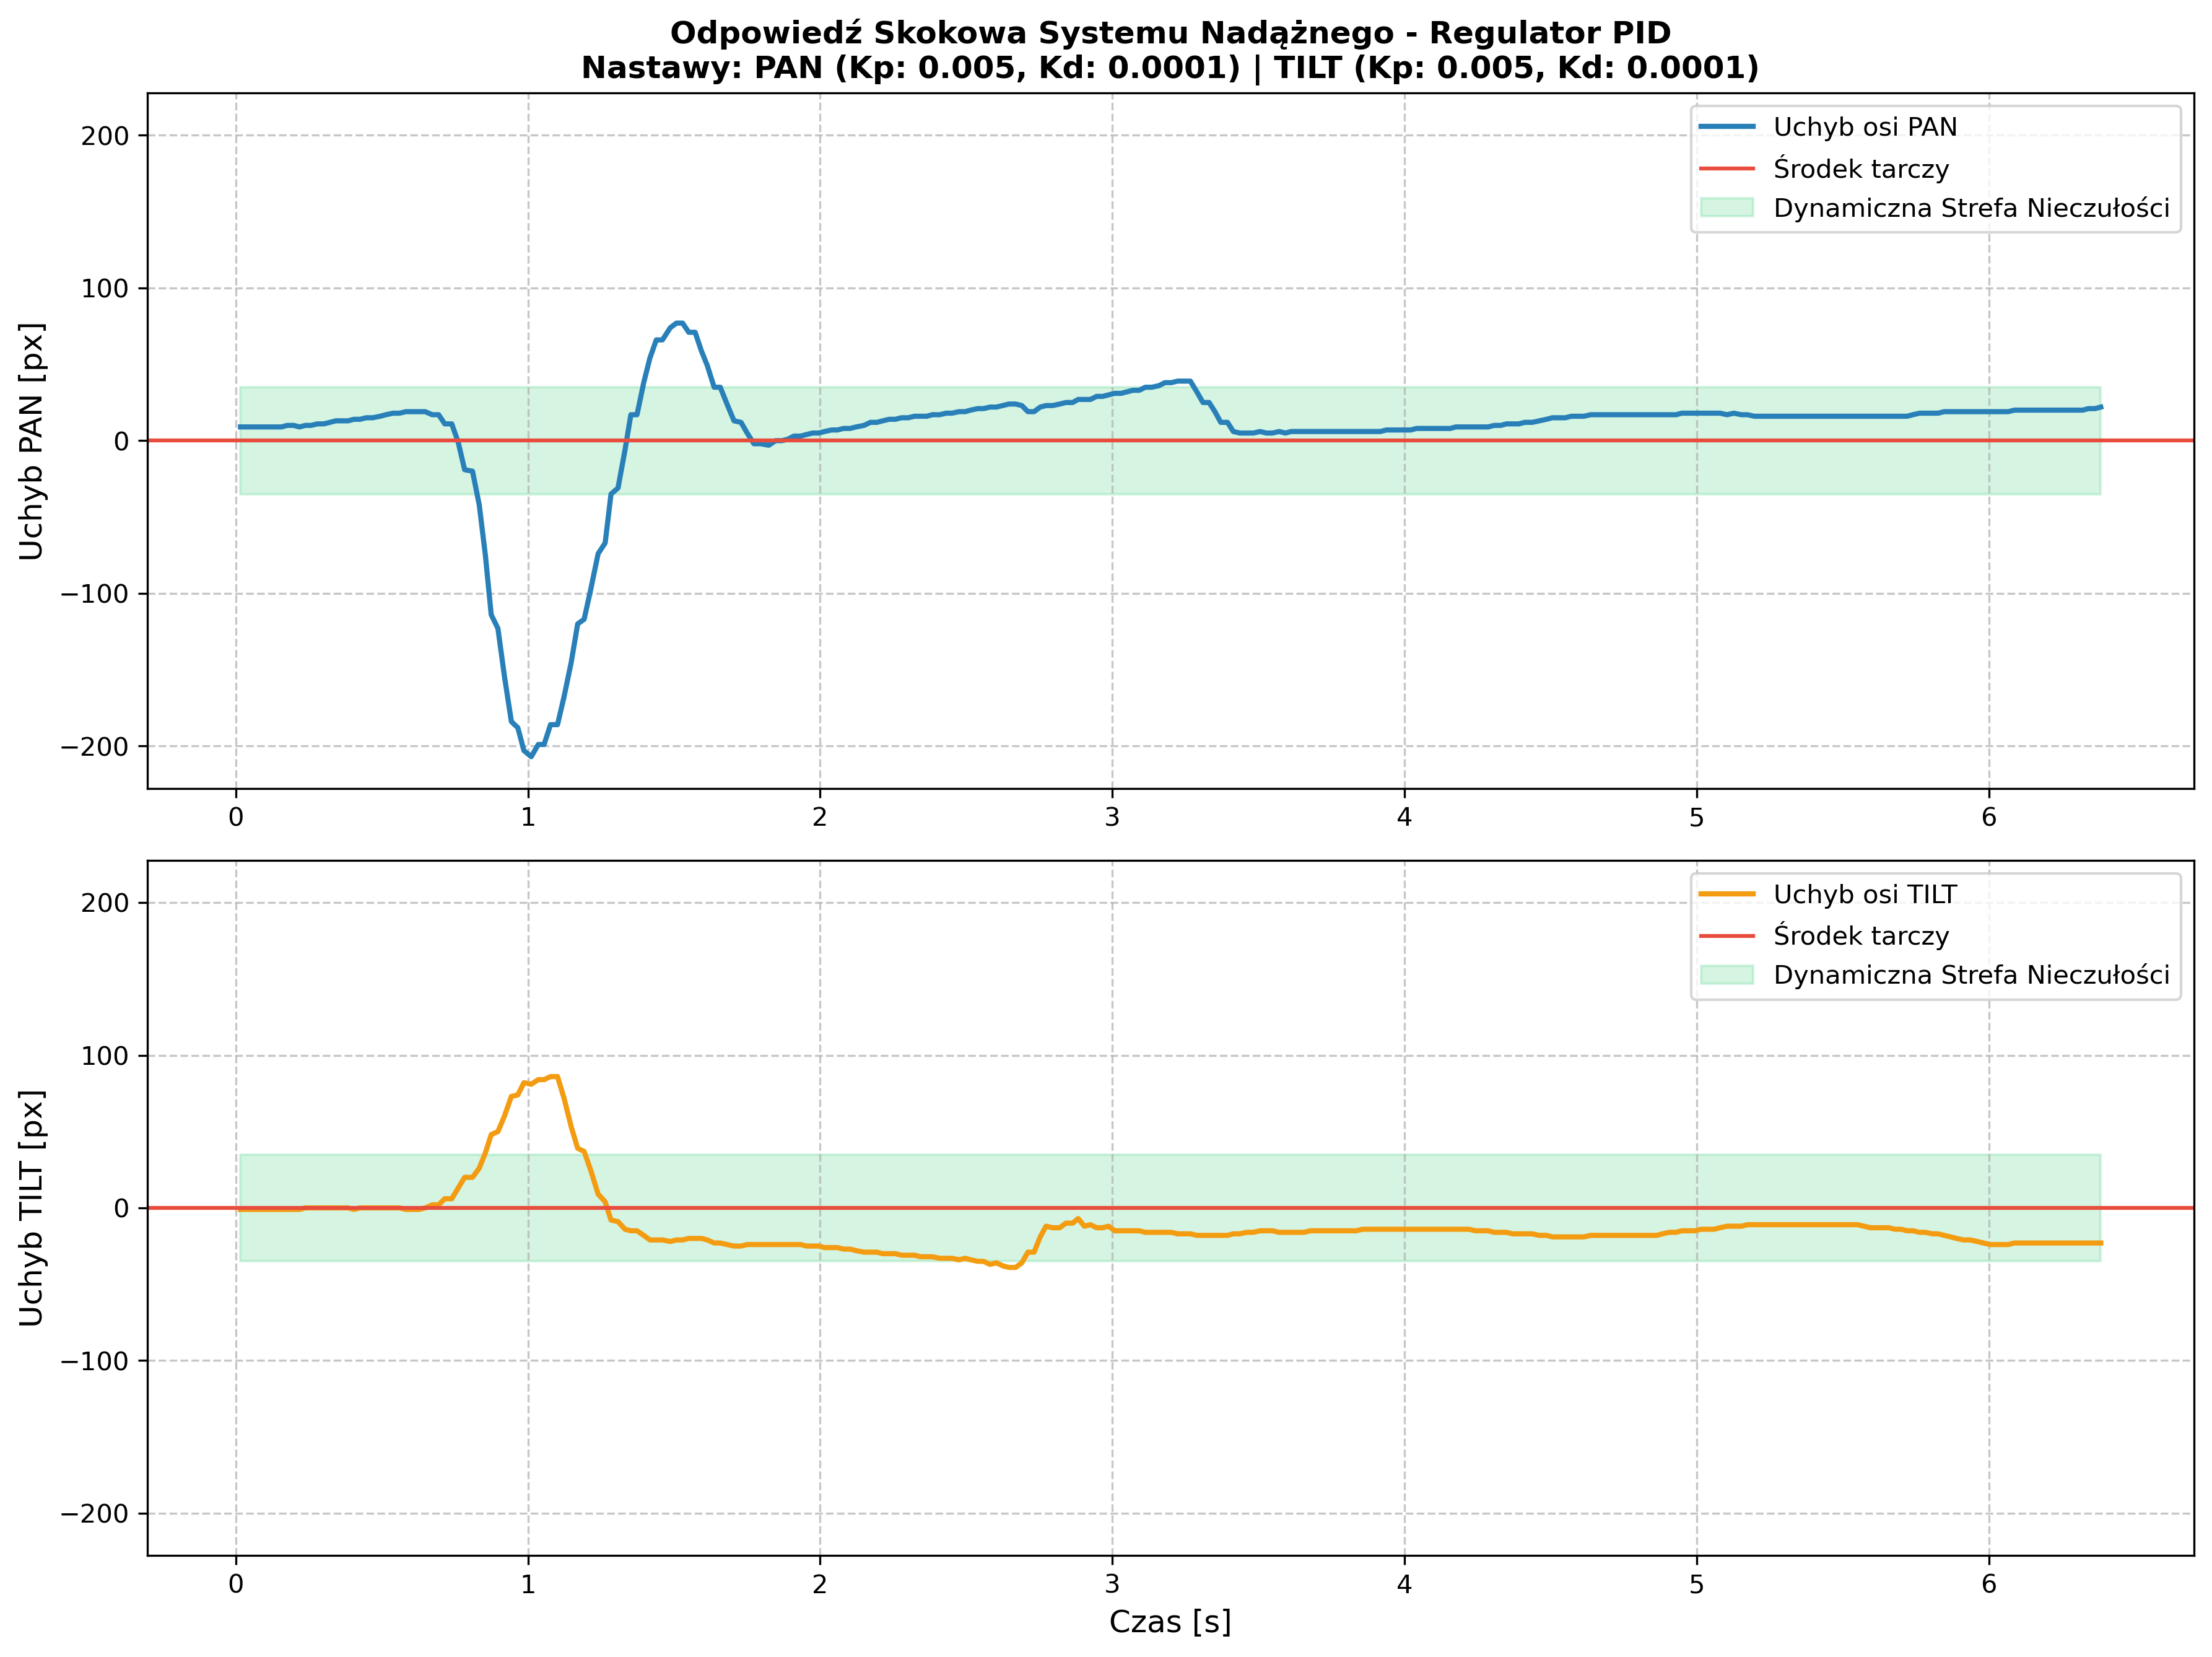
\includegraphics[width=\textwidth]{./Obrazy/Wyniki PID/wykres_GOOD_PID_move_80_cm.png}
    \caption{Nastawy heurystyczne.}
\end{subfigure}
\hfill
\begin{subfigure}{0.48\textwidth}
    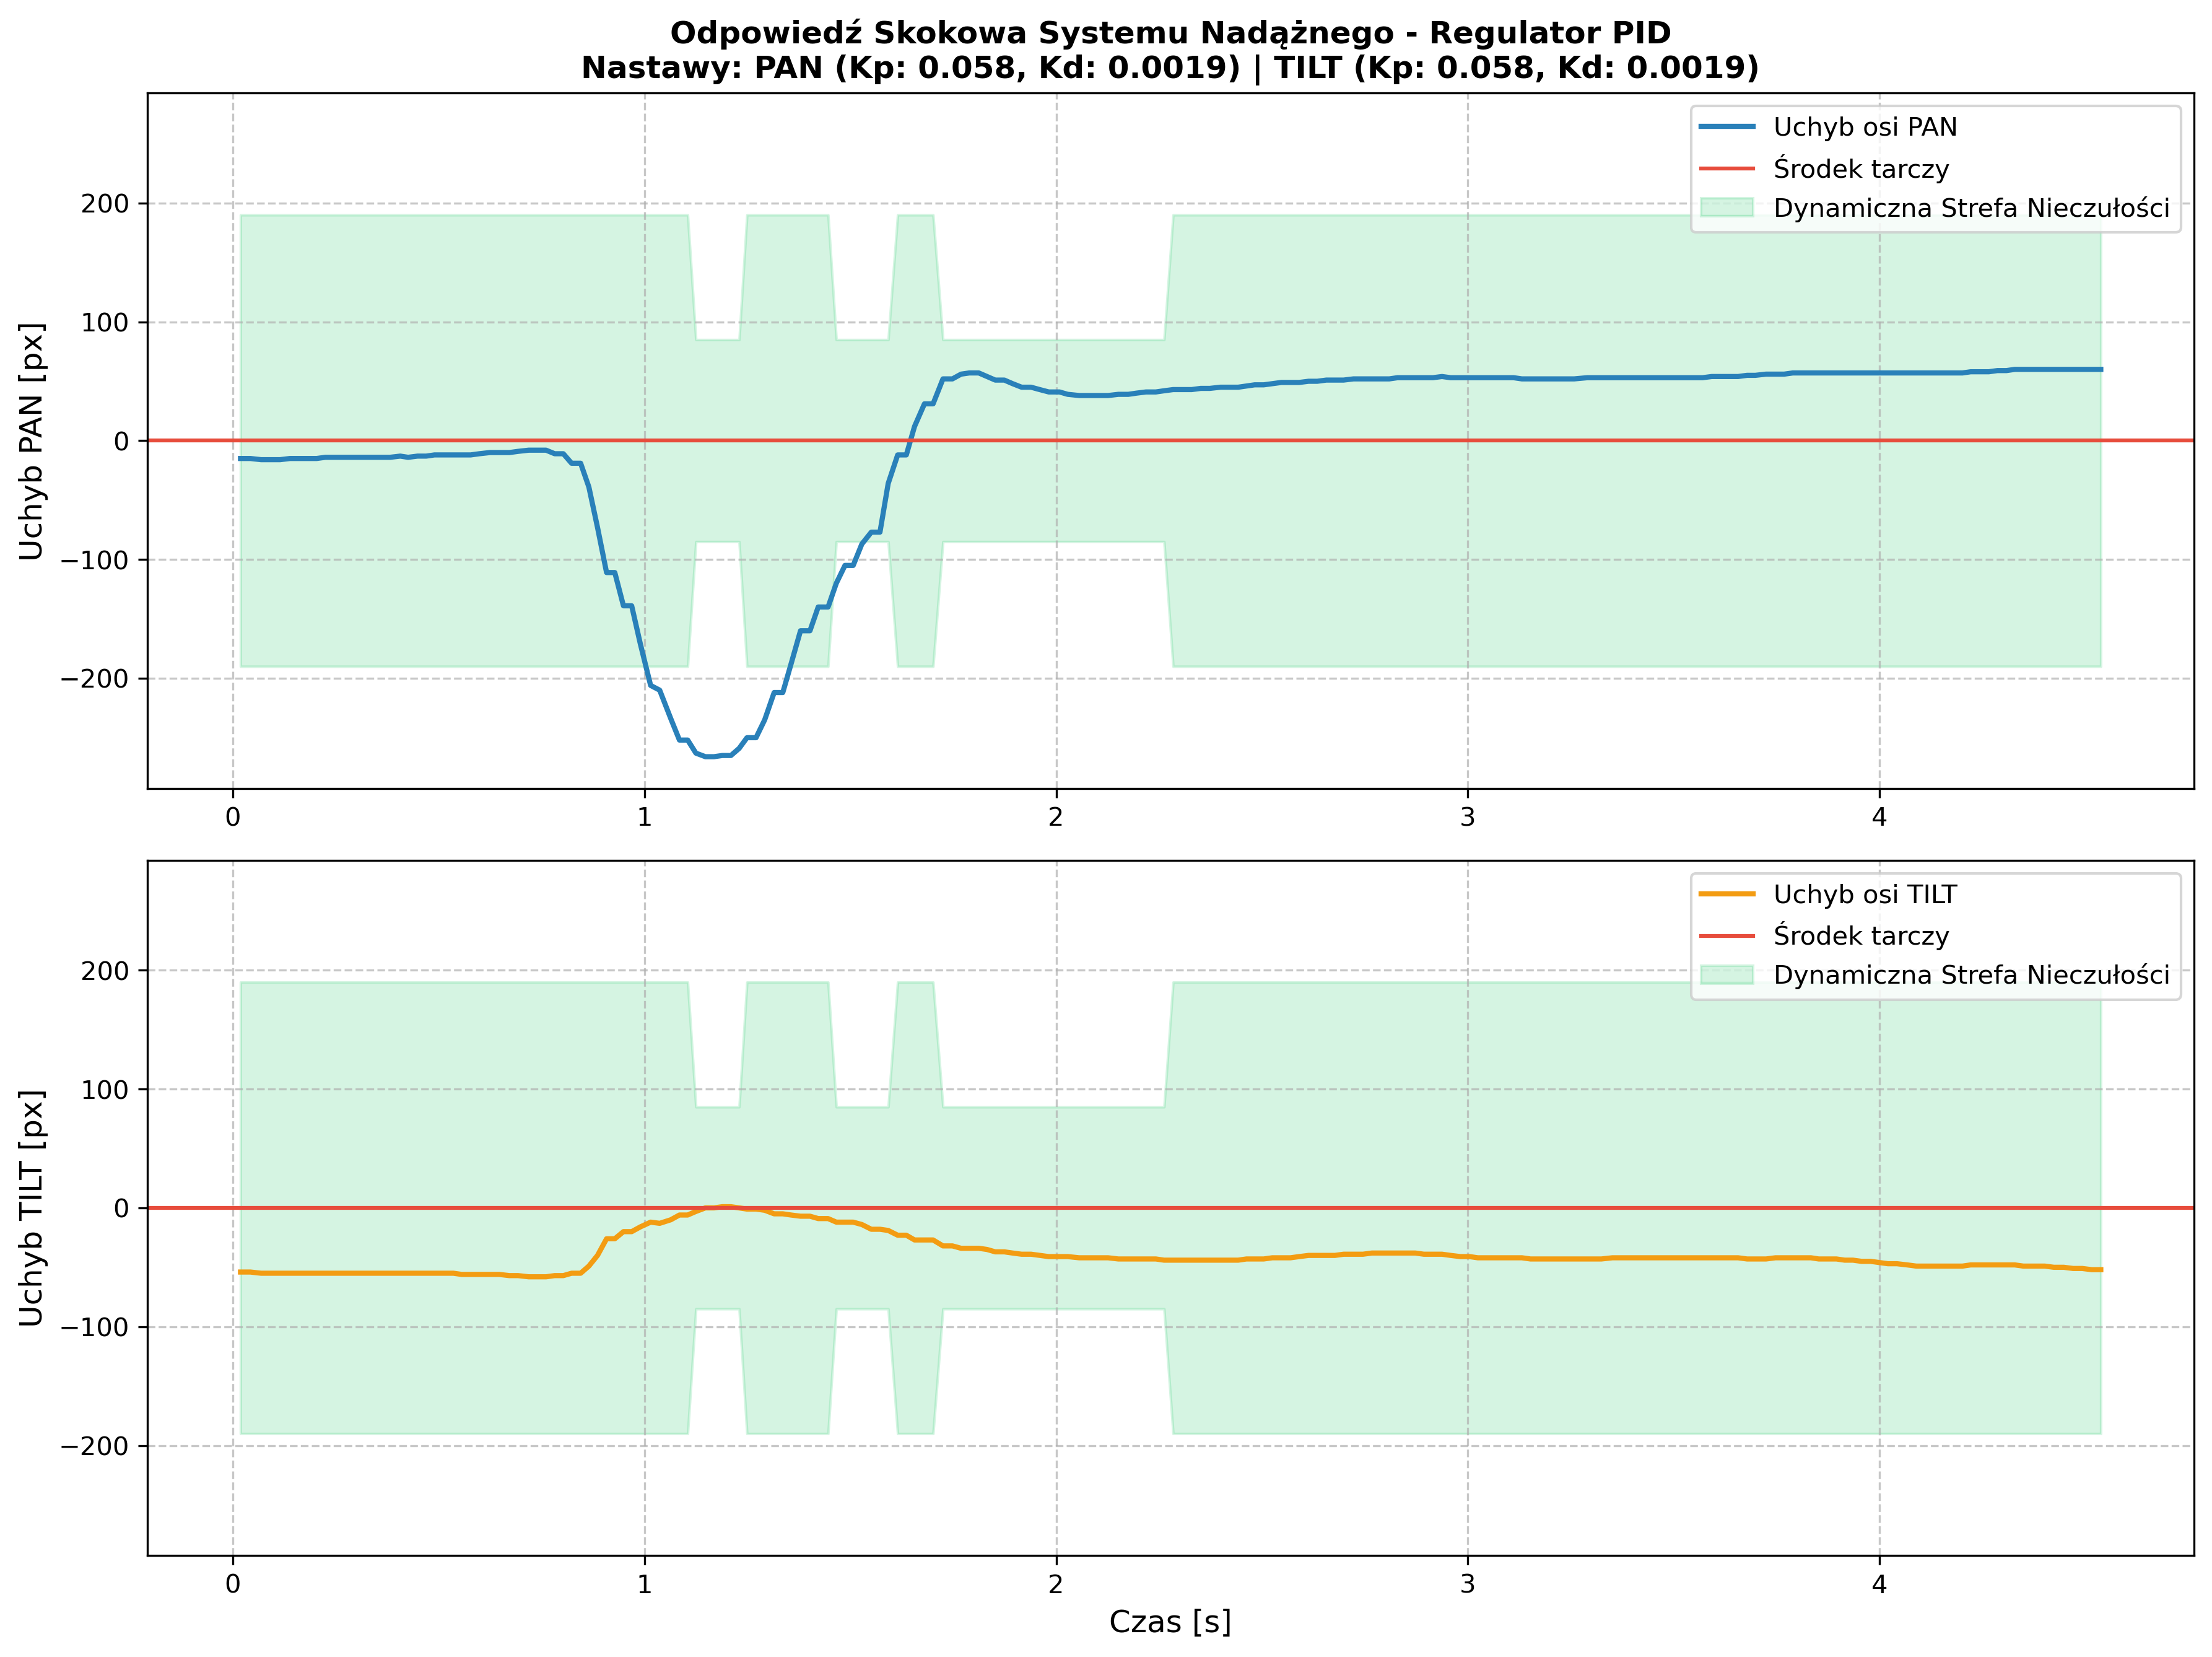
\includegraphics[width=\textwidth]{./Obrazy/Wyniki PID/wykres_UP_PID_move_80_cm.png}
    \caption{Nastawy analityczne.}
\end{subfigure}
\caption{Porównanie odpowiedzi skokowej regulatora PID dla dystansu 80~cm.}
\label{fig:pid_skok_80}
\end{figure}

Zmniejszenie dystansu do $30$~cm (rys. \ref{fig:pid_skok_30}) drastycznie uwypukliło słabości metody heurystycznej. Ze względu na fakt, że z bliska ta sama zmiana fizycznego położenia celu generuje znacznie większą pozorną prędkość kątową na matrycy kamery, układ z nieodpowiednio dobranym tłumieniem wpadł w permanentne, niegasnące oscylacje o dużej amplitudzie. System pracujący na tych nastawach całkowicie utracił stabilność. W tych samych, wysoce wymagających warunkach kinematycznych, regulator z nastawami analitycznymi zachował pełną krzepkość (\textit{robustness}). Mimo niezwykle agresywnego wejścia, wyliczony człon różniczkujący skutecznie wytracił energię kinetyczną układu, sprowadzając obiekt do centrum kadru i zapobiegając oscylacjom.

\begin{figure}[!ht]
\centering
\begin{subfigure}{0.48\textwidth}
    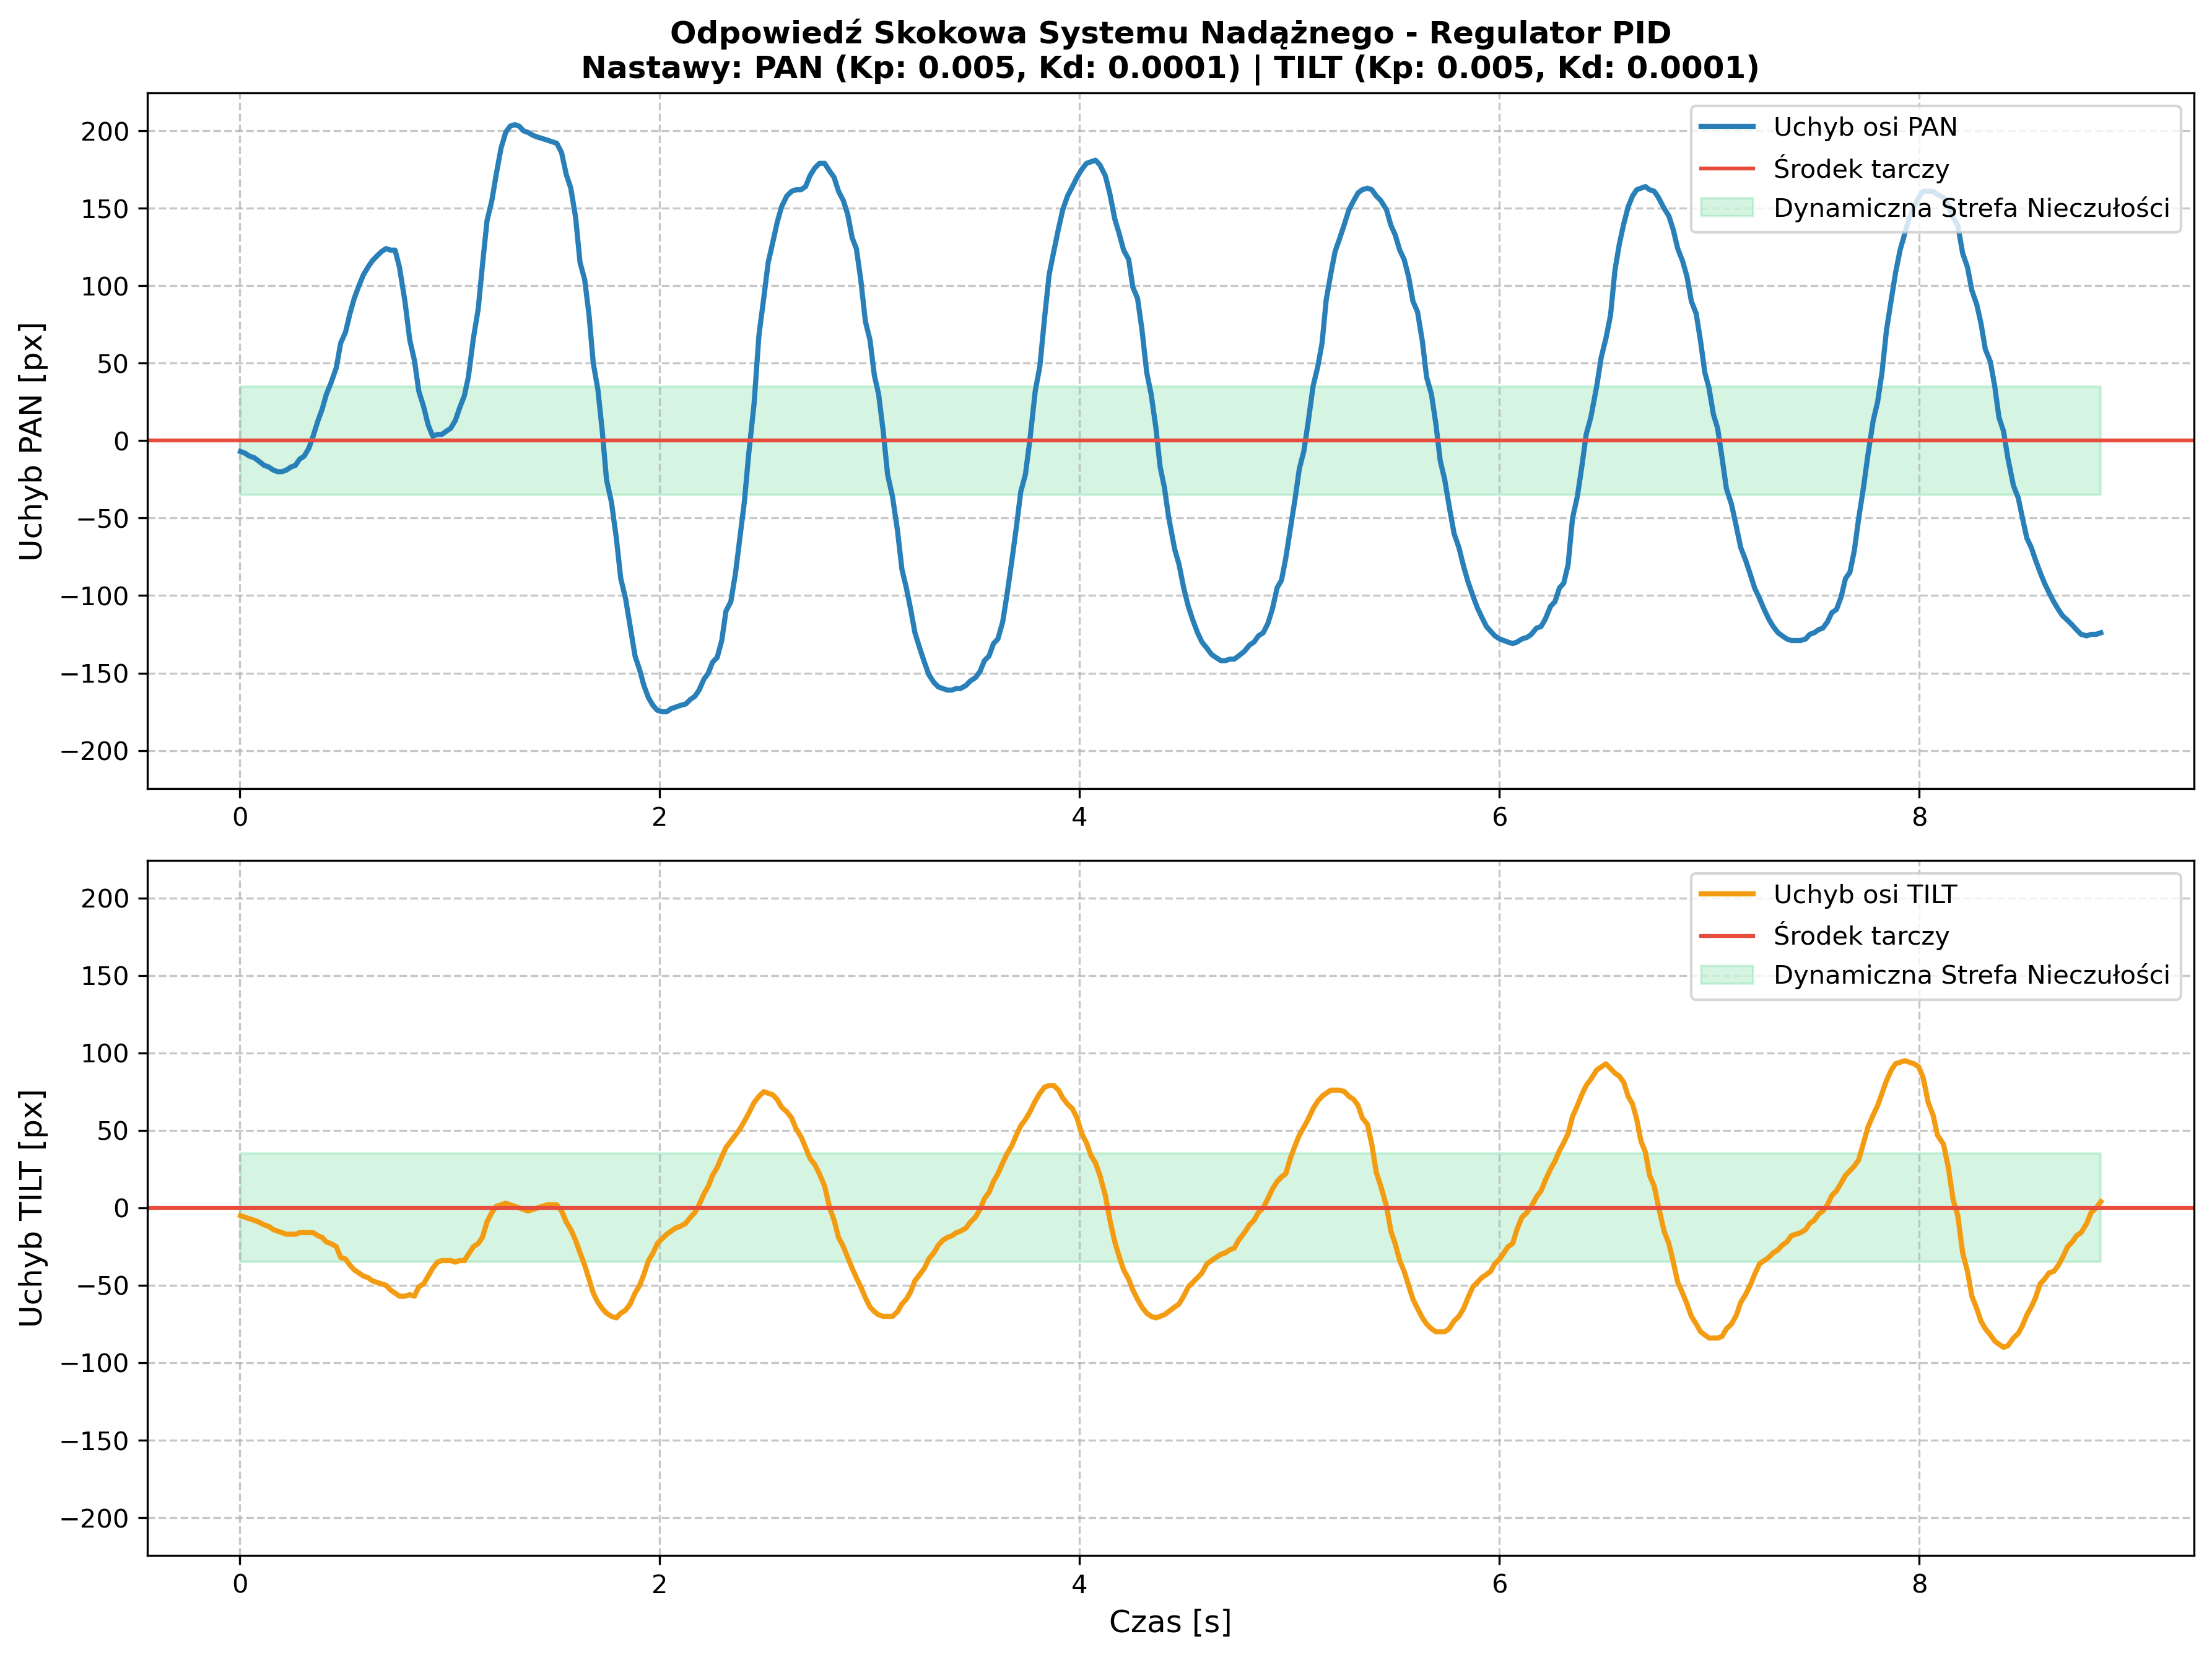
\includegraphics[width=\textwidth]{./Obrazy/Wyniki PID/wykres_GOOD_PID_move_30_cm.png}
    \caption{Nastawy heurystyczne -- utrata stabilności.}
\end{subfigure}
\hfill
\begin{subfigure}{0.48\textwidth}
    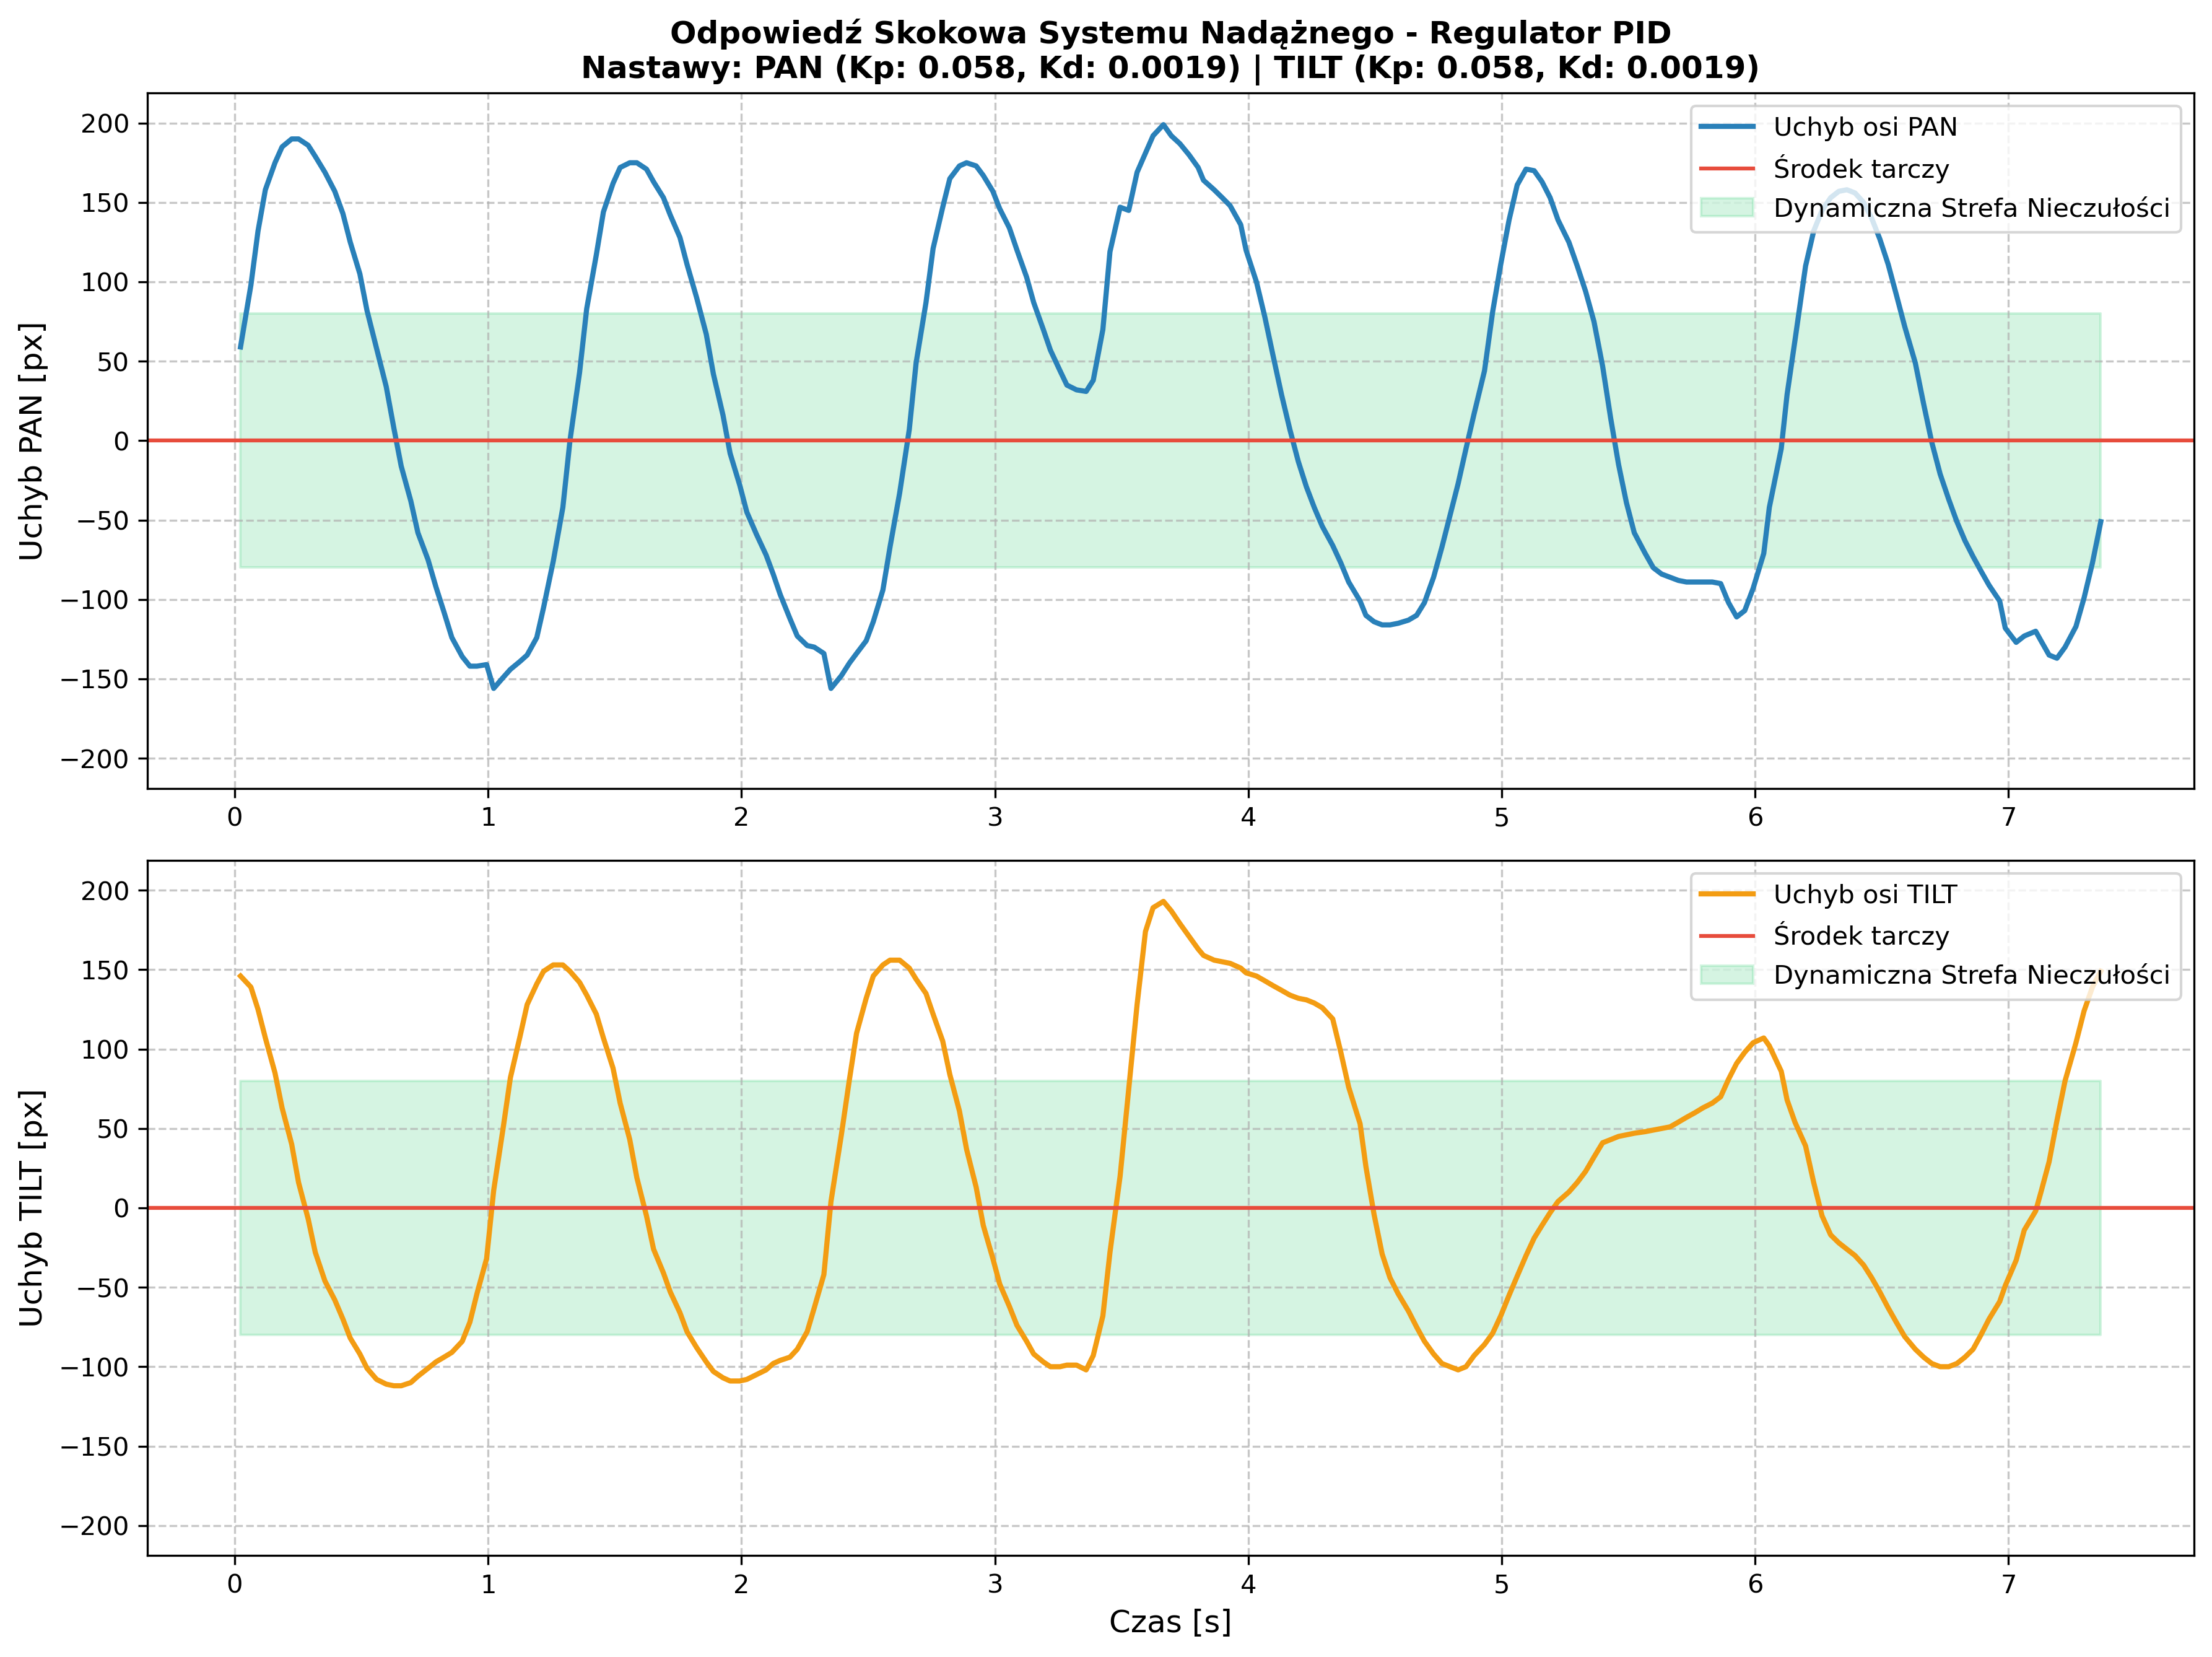
\includegraphics[width=\textwidth]{./Obrazy/Wyniki PID/wykres_UP_PID_move_30_cm.png}
    \caption{Nastawy analityczne -- asymtotyczne tłumienie drgań.}
\end{subfigure}
\caption{Porównanie odpowiedzi skokowej regulatora PID dla dystansu 30~cm.}
\label{fig:pid_skok_30}
\end{figure}

W przypadku dużej odległości równej $150$~cm (rys. \ref{fig:pid_skok_150}), obiekt testowy zajmował ułamek pierwotnej powierzchni obrazu. Nastawy heurystyczne wykazały tu odpowiedź o charakterze mocno aperiodicznym i zachowawczym -- serwomechanizmy zbyt zachowawczo dążyły do celu, co przy szybko poruszających się obiektach skutkowałoby ich zgubieniem z kadru. Wprowadzenie nastaw analitycznych zagwarantowało utrzymanie wysokiej dynamiki i powtarzalności śledzenia. Wykres \ref{fig:pid_skok_150}b potwierdza, że układ szybko dokonał korekty położenia, a adaptacyjnie zawężona strefa nieczułości odpowiednio wcześnie wyzerowała sygnał sterujący, blokując pozycję docelową.

\begin{figure}[!ht]
\centering
\begin{subfigure}{0.48\textwidth}
    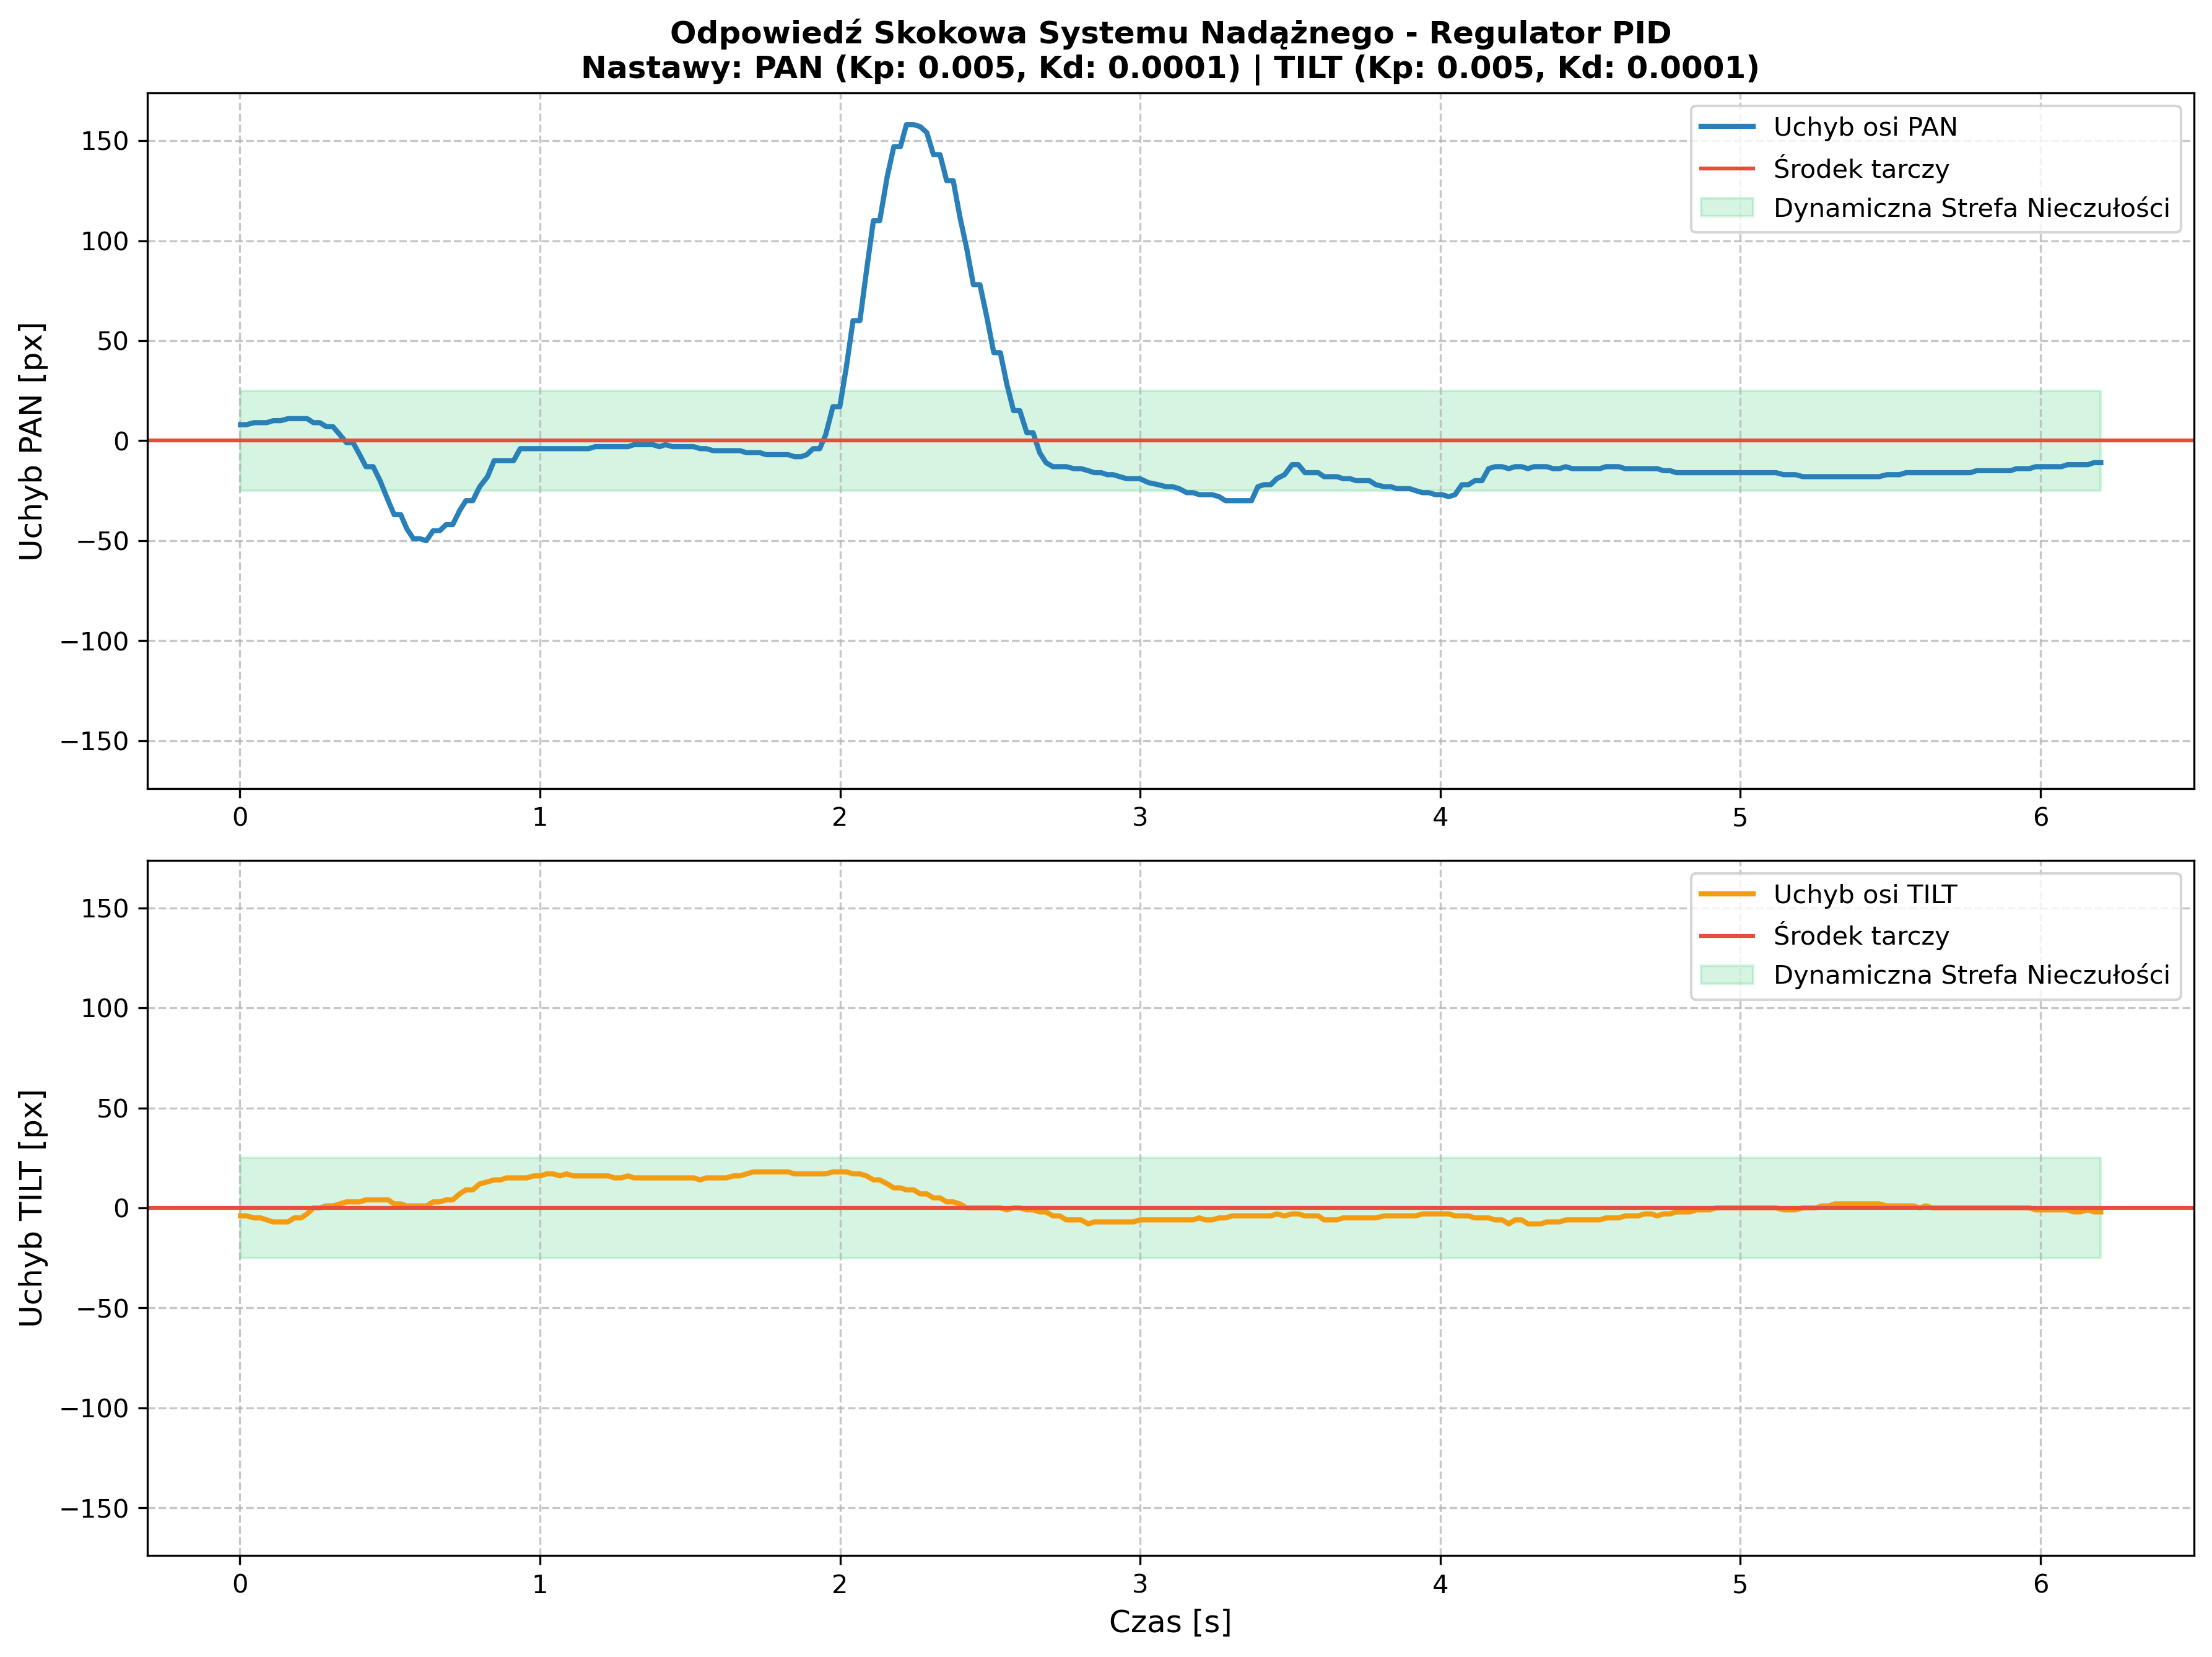
\includegraphics[width=\textwidth]{./Obrazy/Wyniki PID/wykres_GOOD_PID_move_150_cm.png}
    \caption{Nastawy heurystyczne.}
\end{subfigure}
\hfill
\begin{subfigure}{0.48\textwidth}
    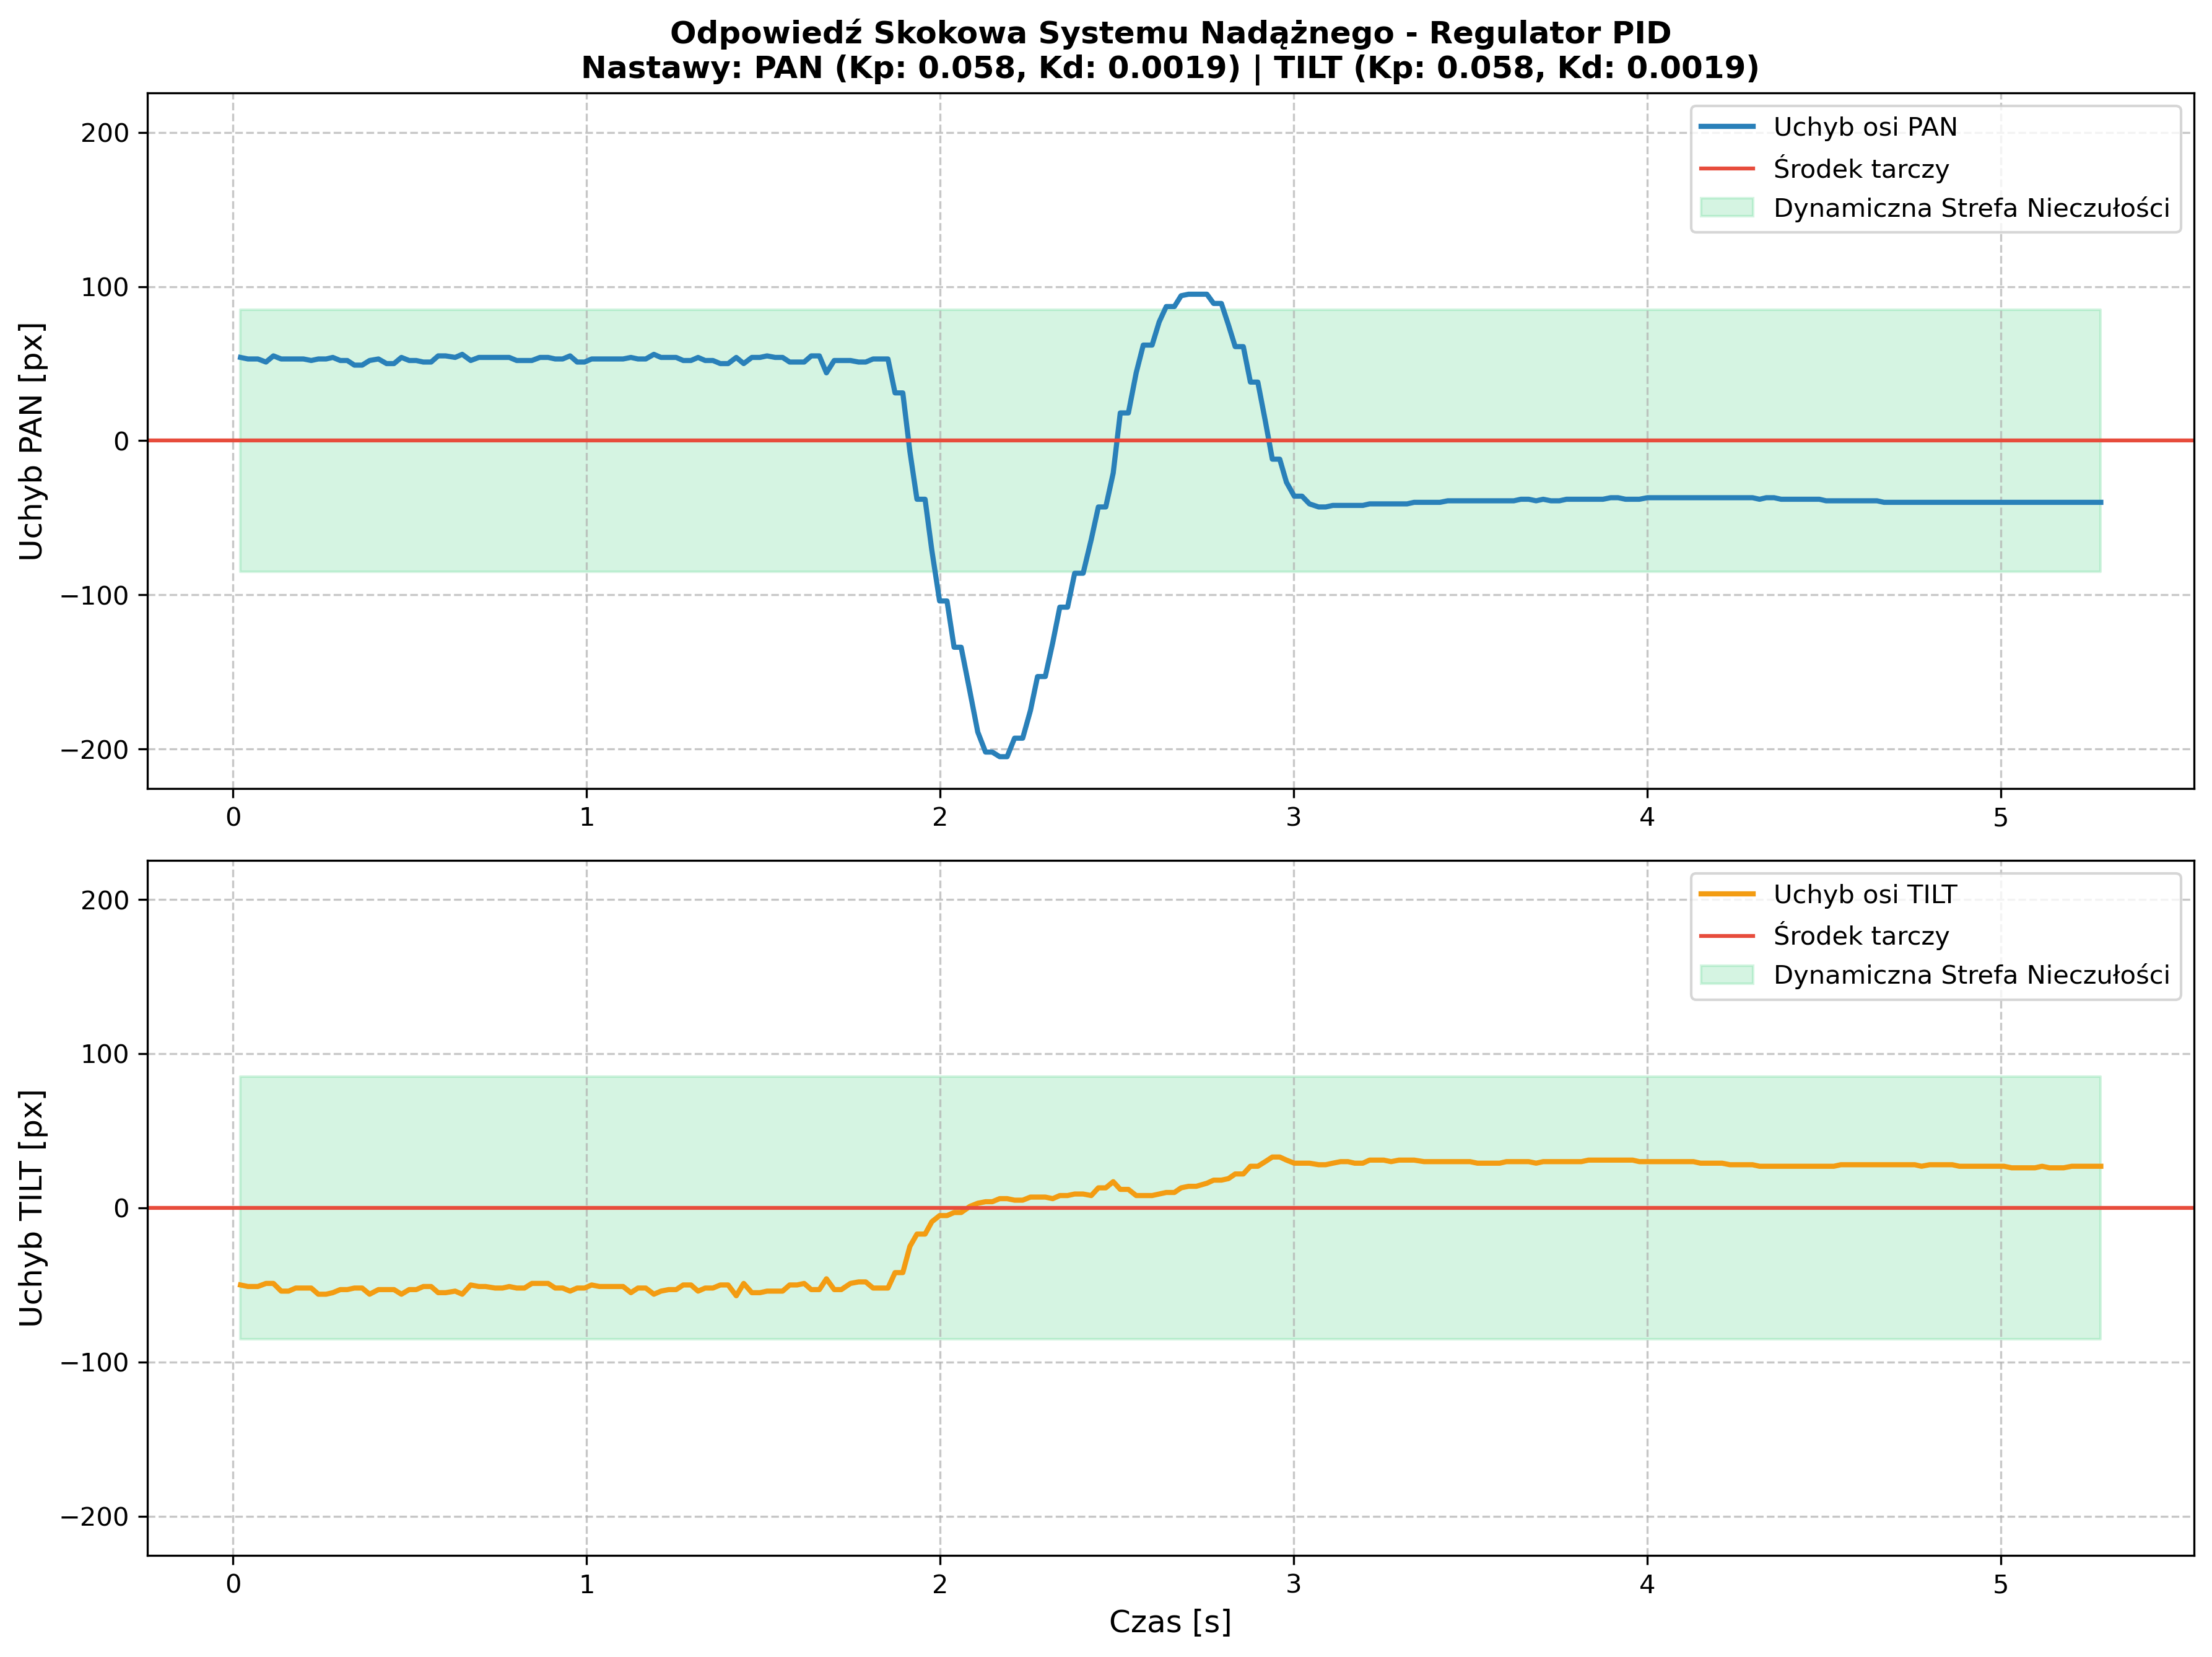
\includegraphics[width=\textwidth]{./Obrazy/Wyniki PID/wykres_UP_PID_move_150_cm.png}
    \caption{Nastawy analityczne.}
\end{subfigure}
\caption{Porównanie odpowiedzi skokowej regulatora PID dla dystansu 150~cm.}
\label{fig:pid_skok_150}
\end{figure}

\subsection{Śledzenie obiektu poruszającego się po trajektorii okrężnej}
\label{subsec:pid_okrag}

Ruch okrężny ujawnił, że agresywne nastawy heurystyczne powodują szarpanie trajektorii.

\begin{figure}[!ht]
\centering
\begin{subfigure}{0.48\textwidth}
    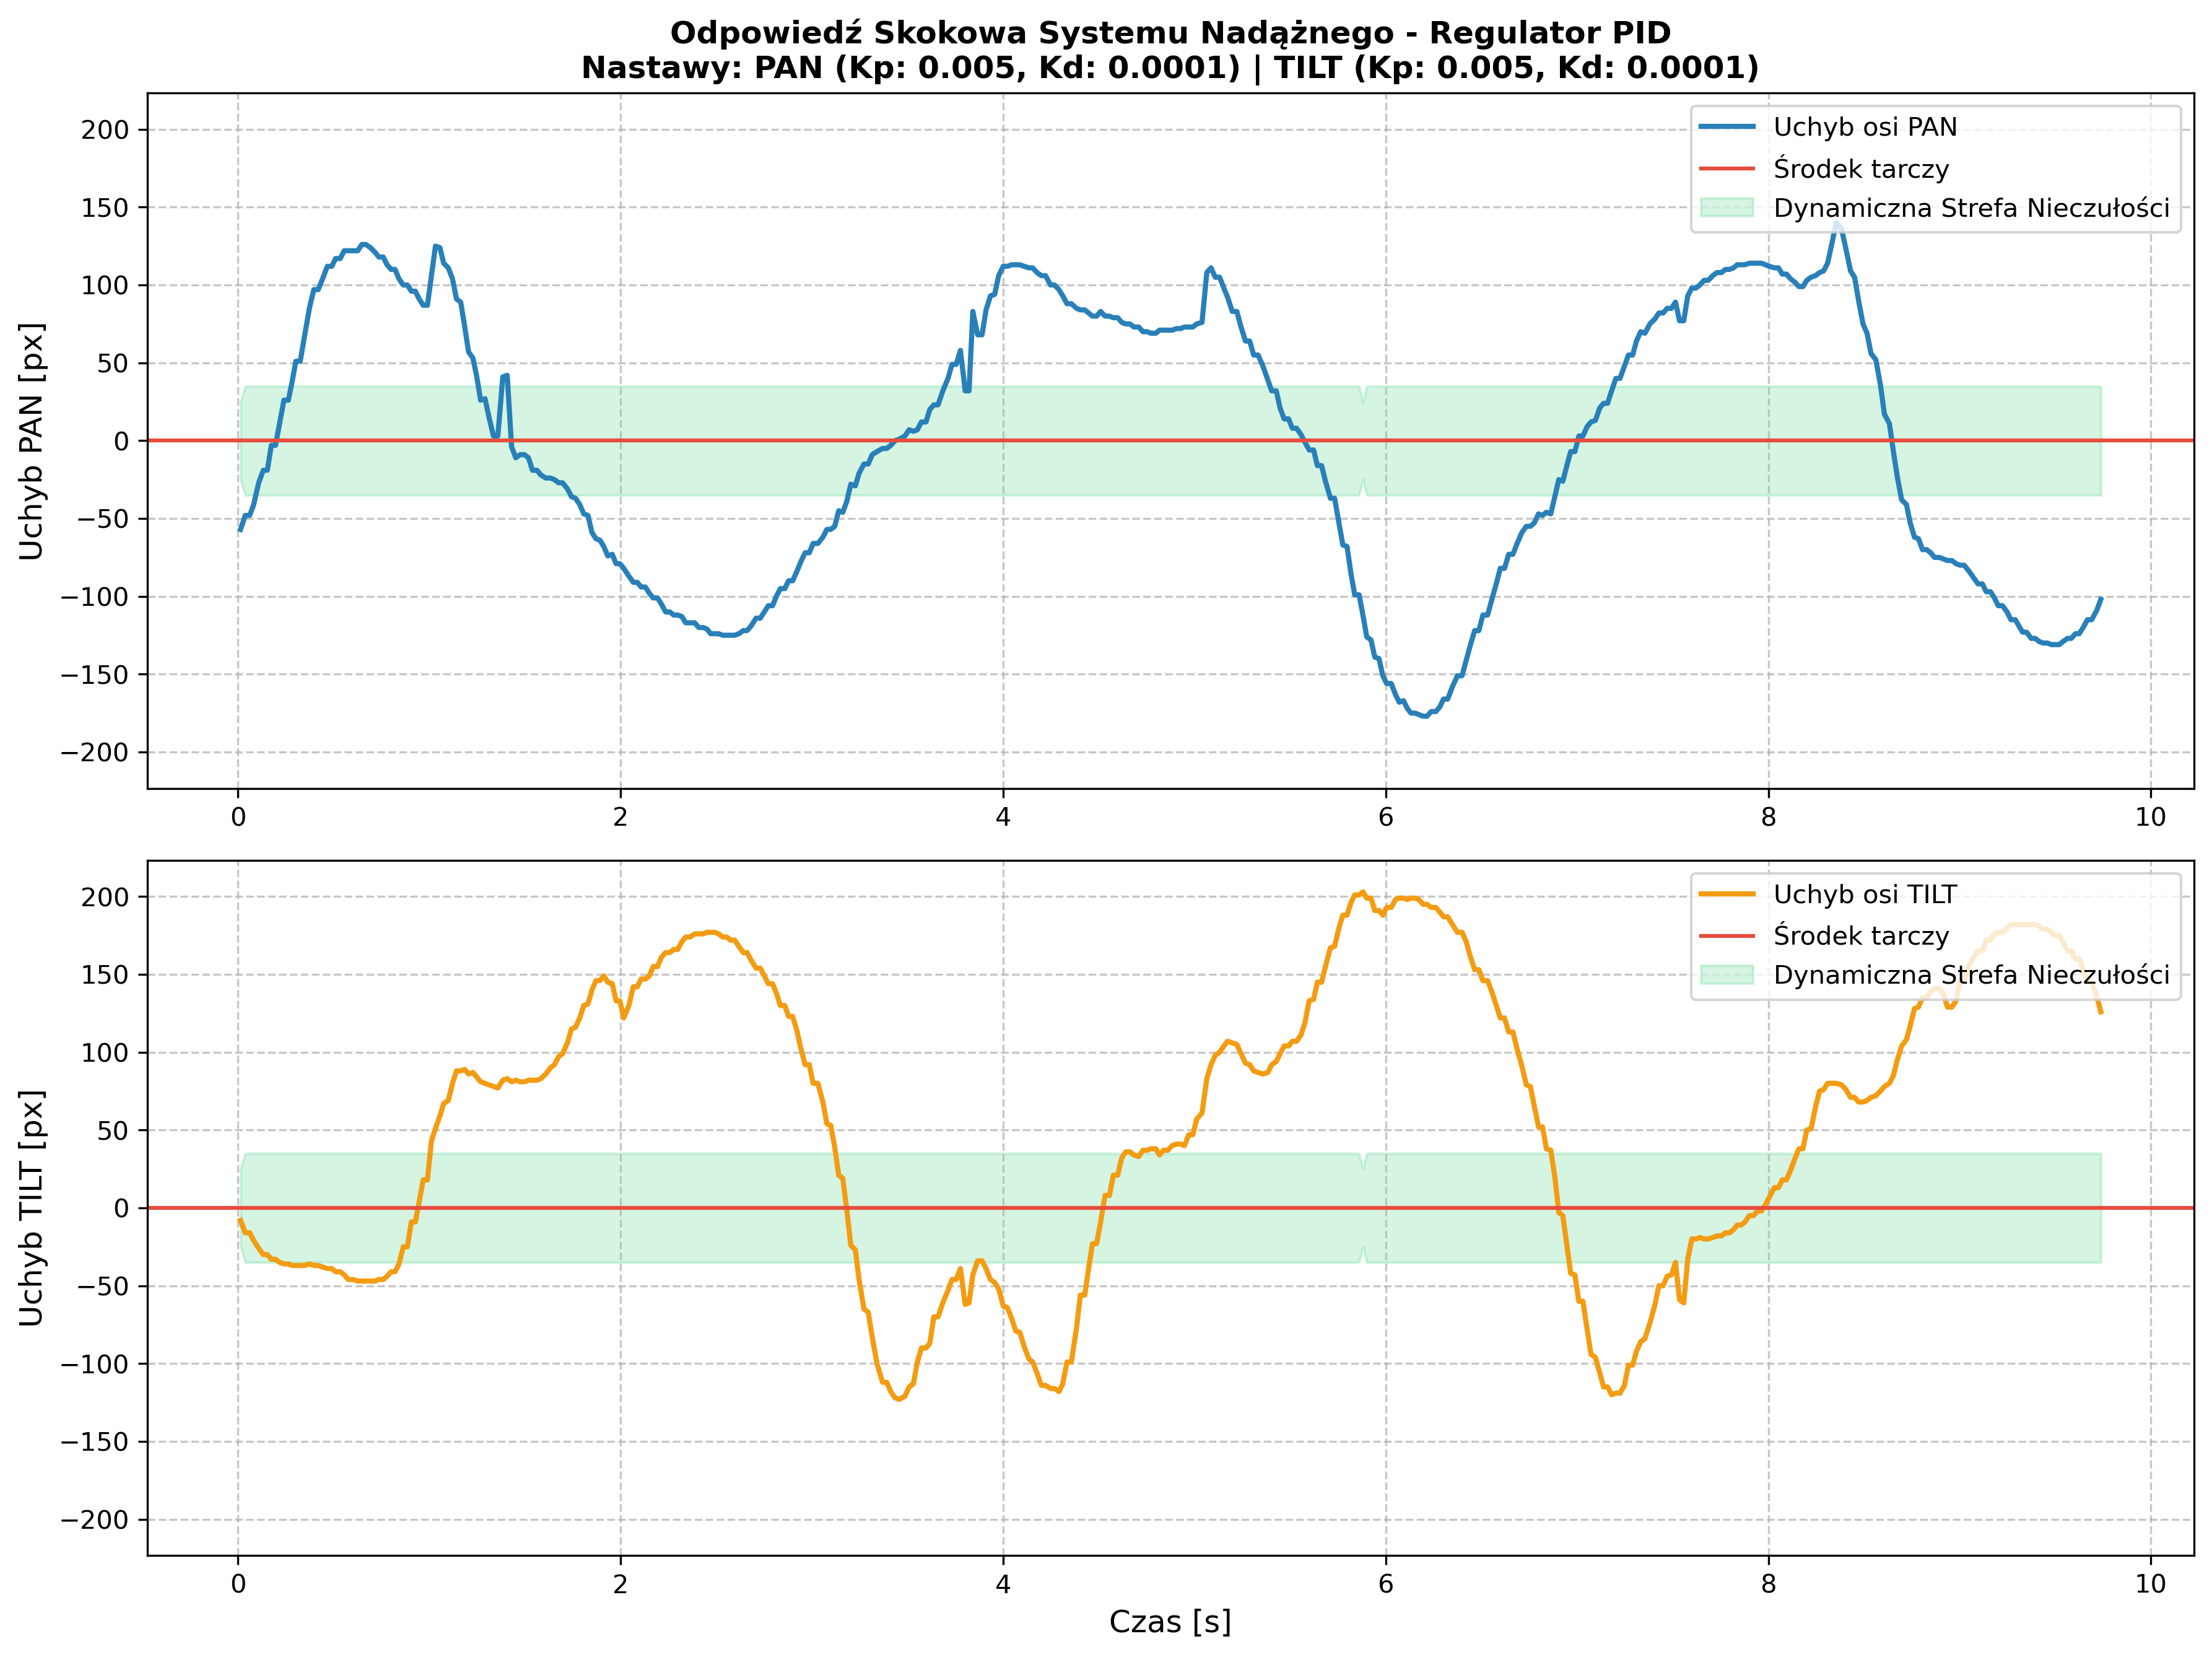
\includegraphics[width=\textwidth]{./Obrazy/Wyniki PID/wykres_GOOD_PID_circural_80_cm.png}
    \caption{Nastawy heurystyczne.}
\end{subfigure}
\hfill
\begin{subfigure}{0.48\textwidth}
    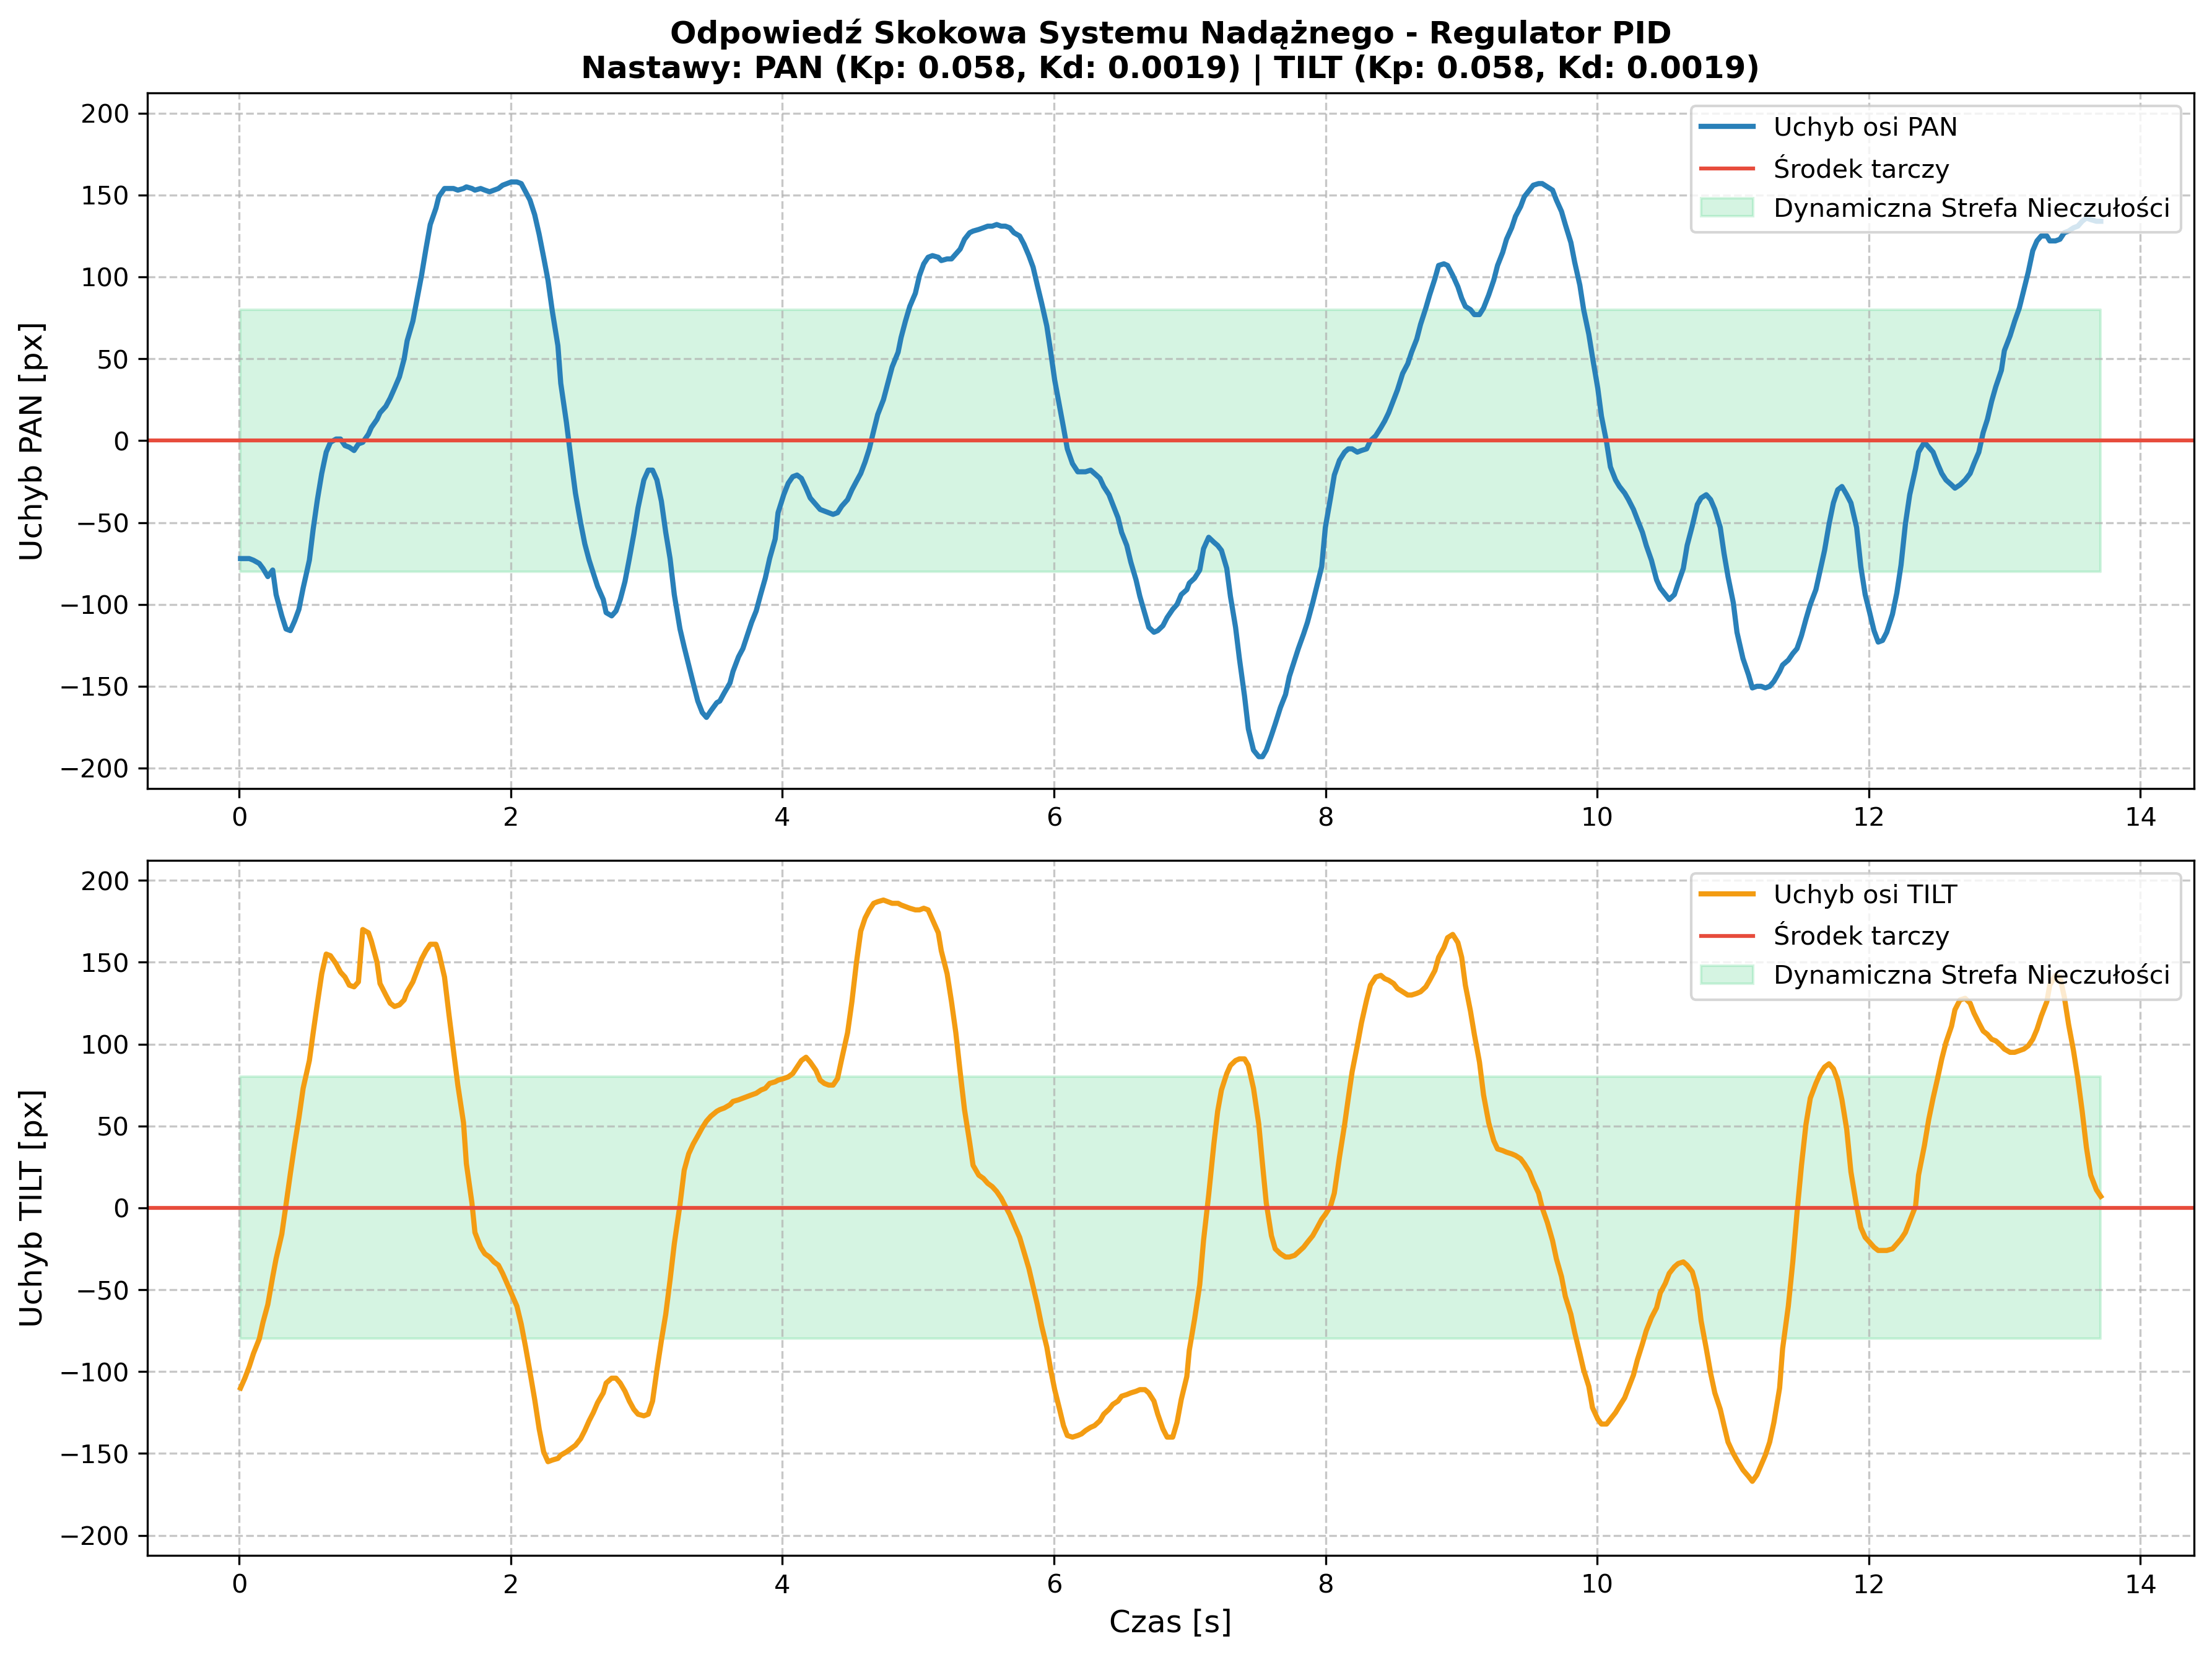
\includegraphics[width=\textwidth]{./Obrazy/Wyniki PID/wykres_UP_PID_circural_80_cm.png}
    \caption{Nastawy analityczne.}
\end{subfigure}
\caption{Śledzenie ruchu okrężnego dla dystansu 80~cm (PID).}
\label{fig:pid_okrag_80}
\end{figure}

\begin{figure}[!ht]
\centering
\begin{subfigure}{0.48\textwidth}
    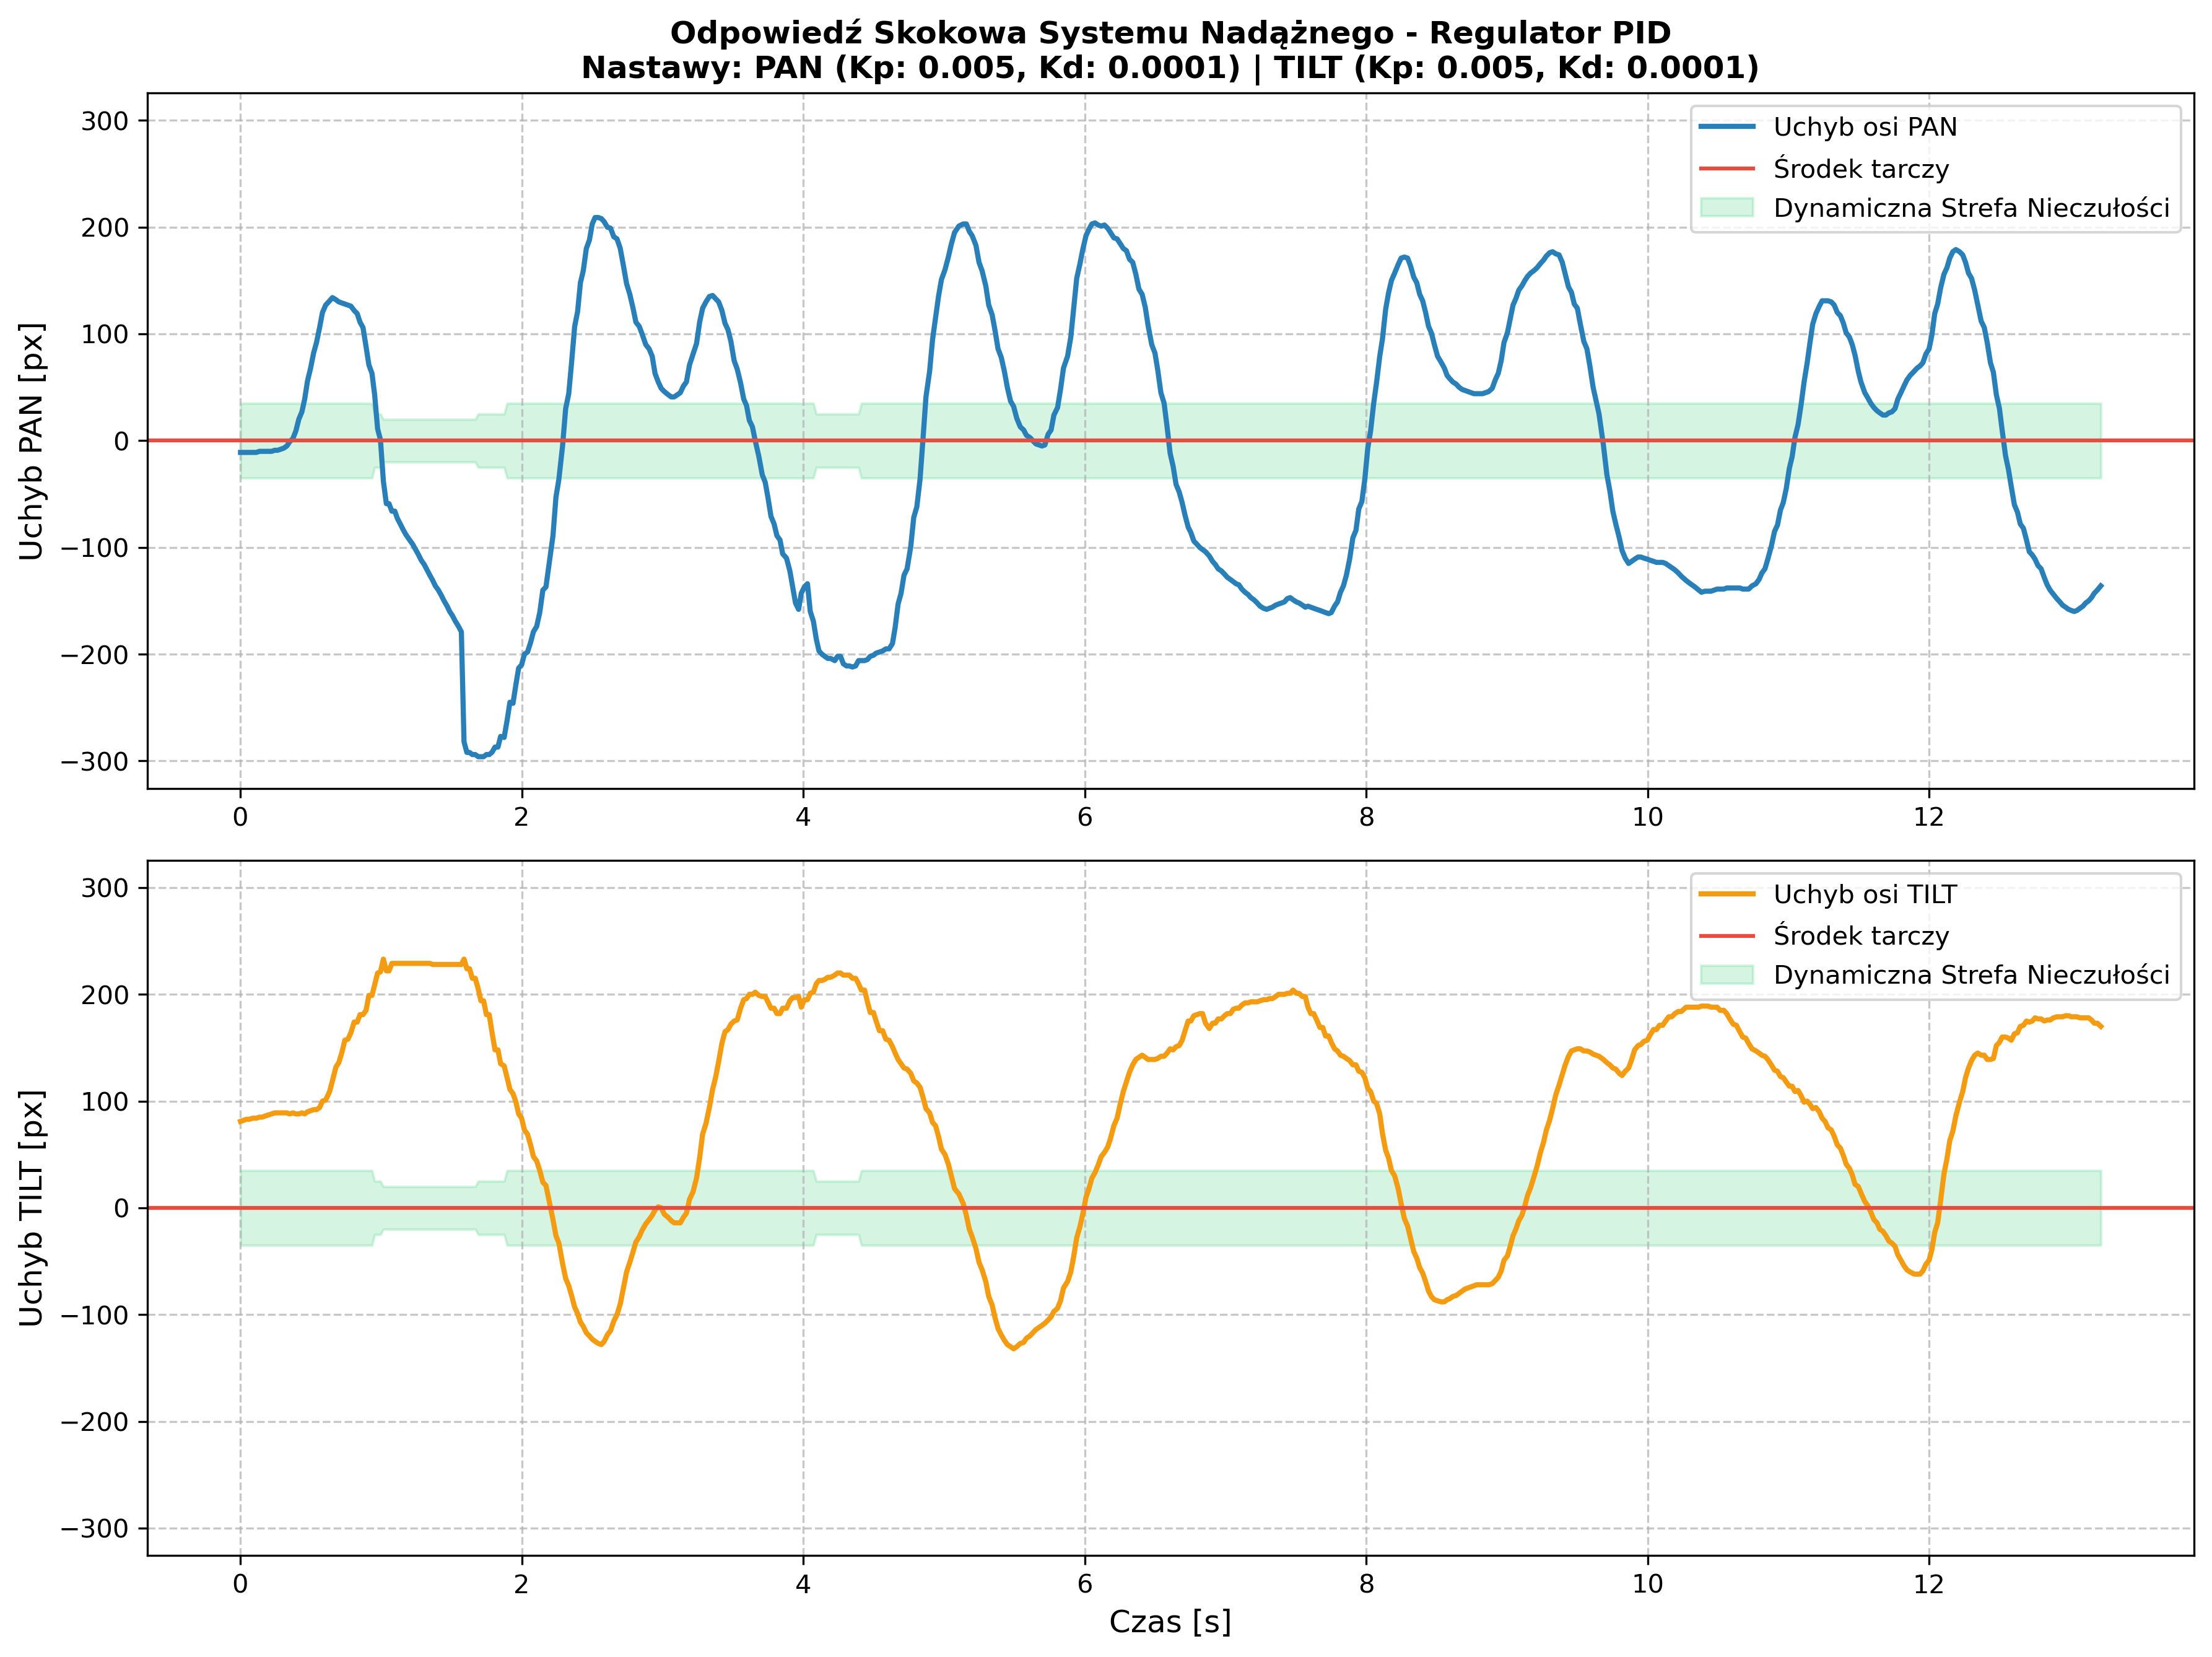
\includegraphics[width=\textwidth]{./Obrazy/Wyniki PID/wykres_GOOD_PID_circural_30_cm.png}
    \caption{Nastawy heurystyczne.}
\end{subfigure}
\hfill
\begin{subfigure}{0.48\textwidth}
    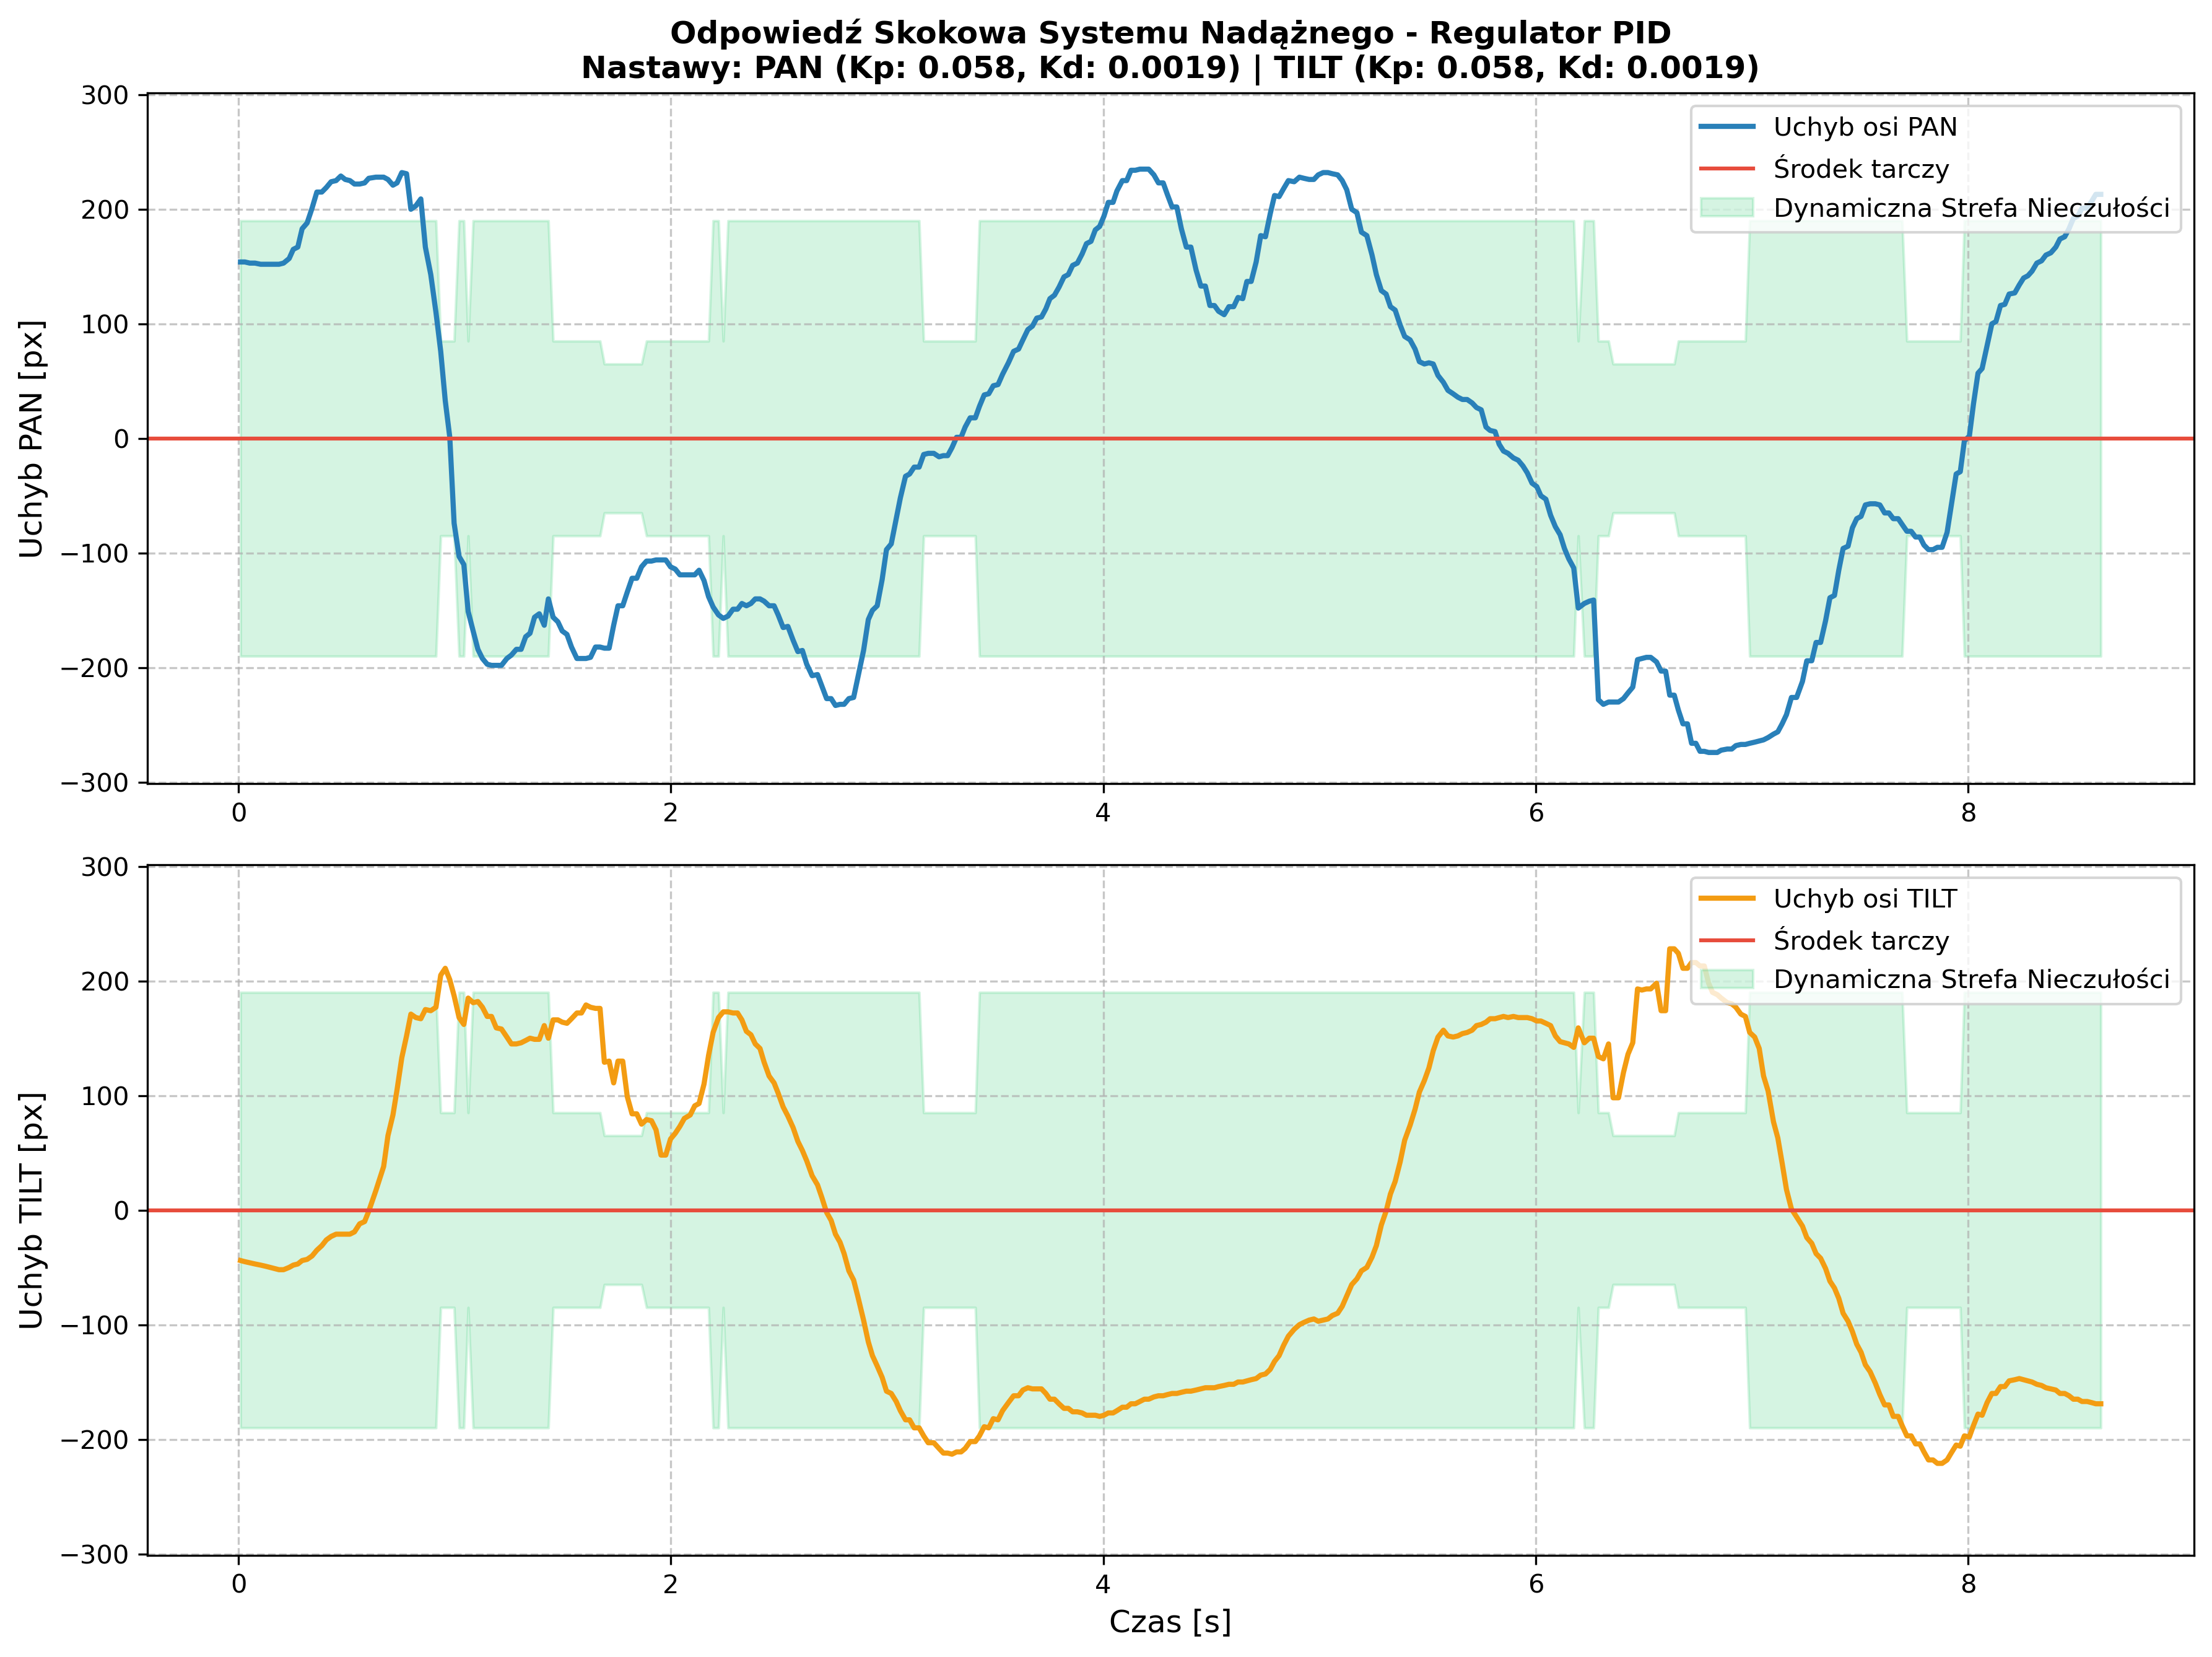
\includegraphics[width=\textwidth]{./Obrazy/Wyniki PID/wykres_UP_PID_circural_30_cm.png}
    \caption{Nastawy analityczne.}
\end{subfigure}
\caption{Śledzenie ruchu okrężnego dla dystansu 30~cm (PID).}
\label{fig:pid_okrag_30}
\end{figure}

\begin{figure}[!ht]
\centering
\begin{subfigure}{0.48\textwidth}
    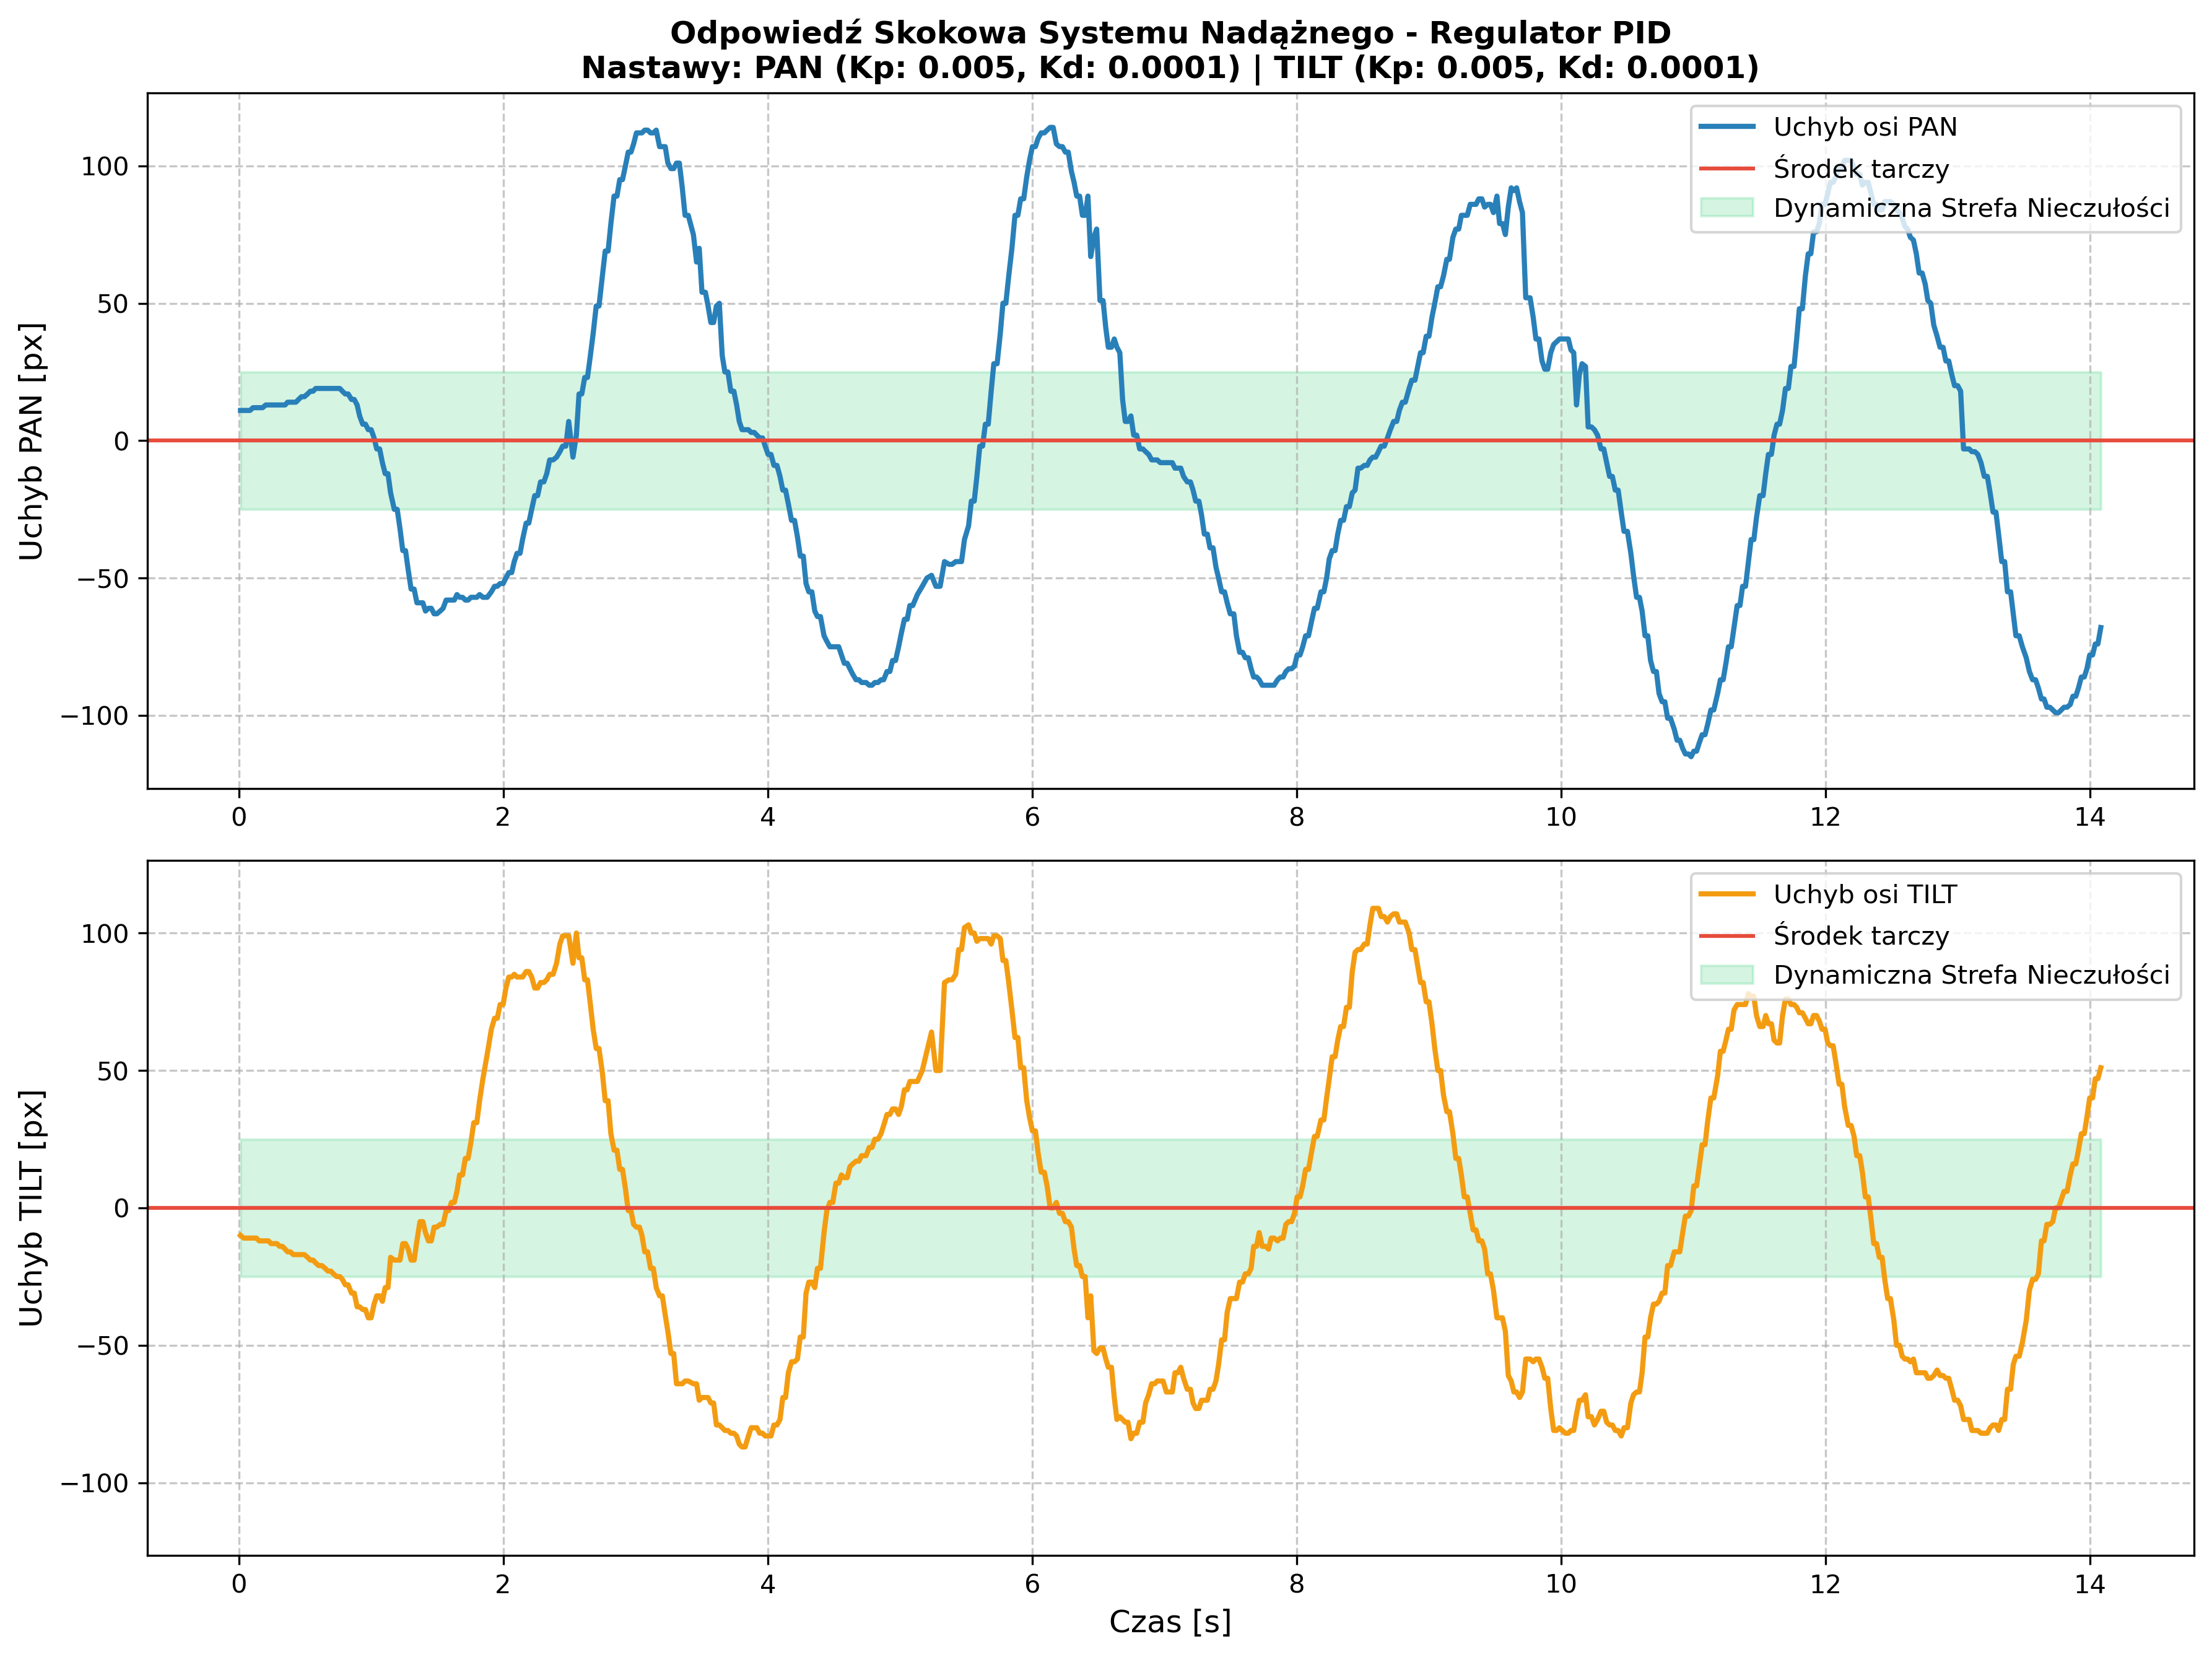
\includegraphics[width=\textwidth]{./Obrazy/Wyniki PID/wykres_GOOD_PID_circural_150_cm.png}
    \caption{Nastawy heurystyczne.}
\end{subfigure}
\hfill
\begin{subfigure}{0.48\textwidth}
    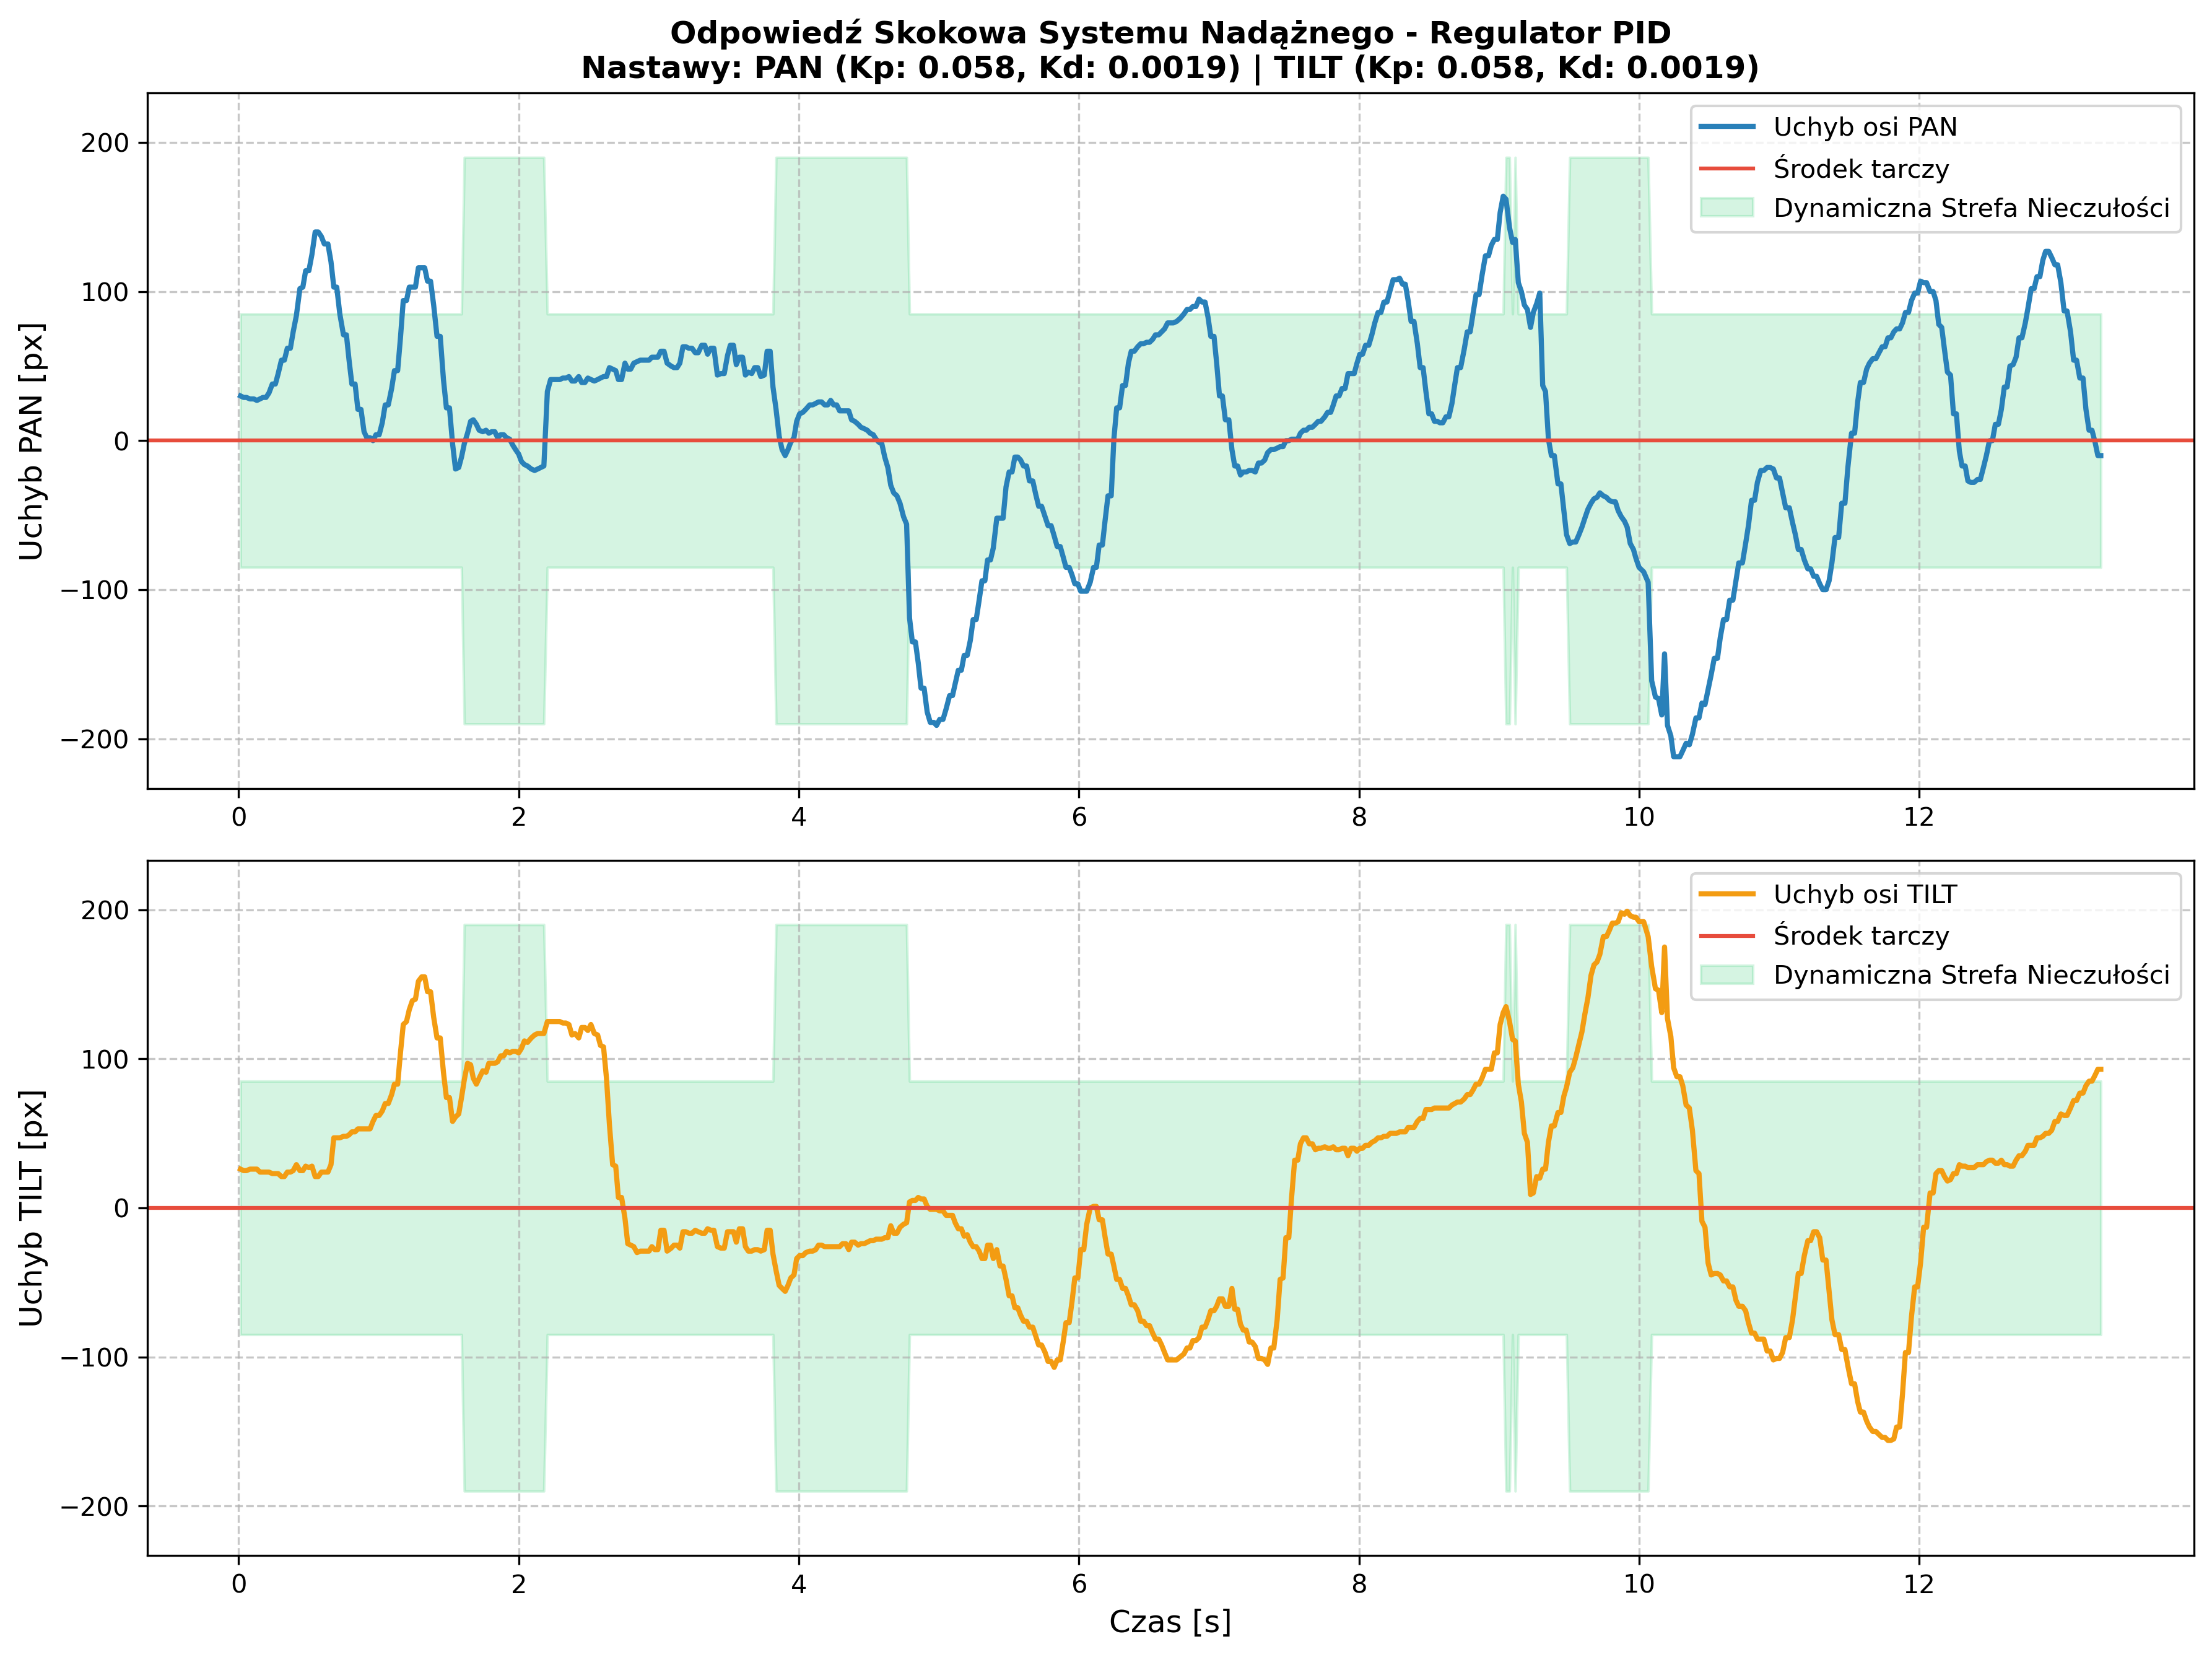
\includegraphics[width=\textwidth]{./Obrazy/Wyniki PID/wykres_UP_PID_circural_150_cm.png}
    \caption{Nastawy analityczne.}
\end{subfigure}
\caption{Śledzenie ruchu okrężnego dla dystansu 150~cm (PID).}
\label{fig:pid_okrag_150}
\end{figure}

\subsection{Test płynnej zmiany dystansu i weryfikacja algorytmu Gain Scheduling}
\label{subsec:pid_oddalanie}

Przy oddalaniu bez adaptacji parametrów układ tracił stabilność. Zastosowanie algorytmu Gain Scheduling zapewniło płynność śledzenia.

\begin{figure}[!ht]
\centering
\begin{subfigure}{0.48\textwidth}
    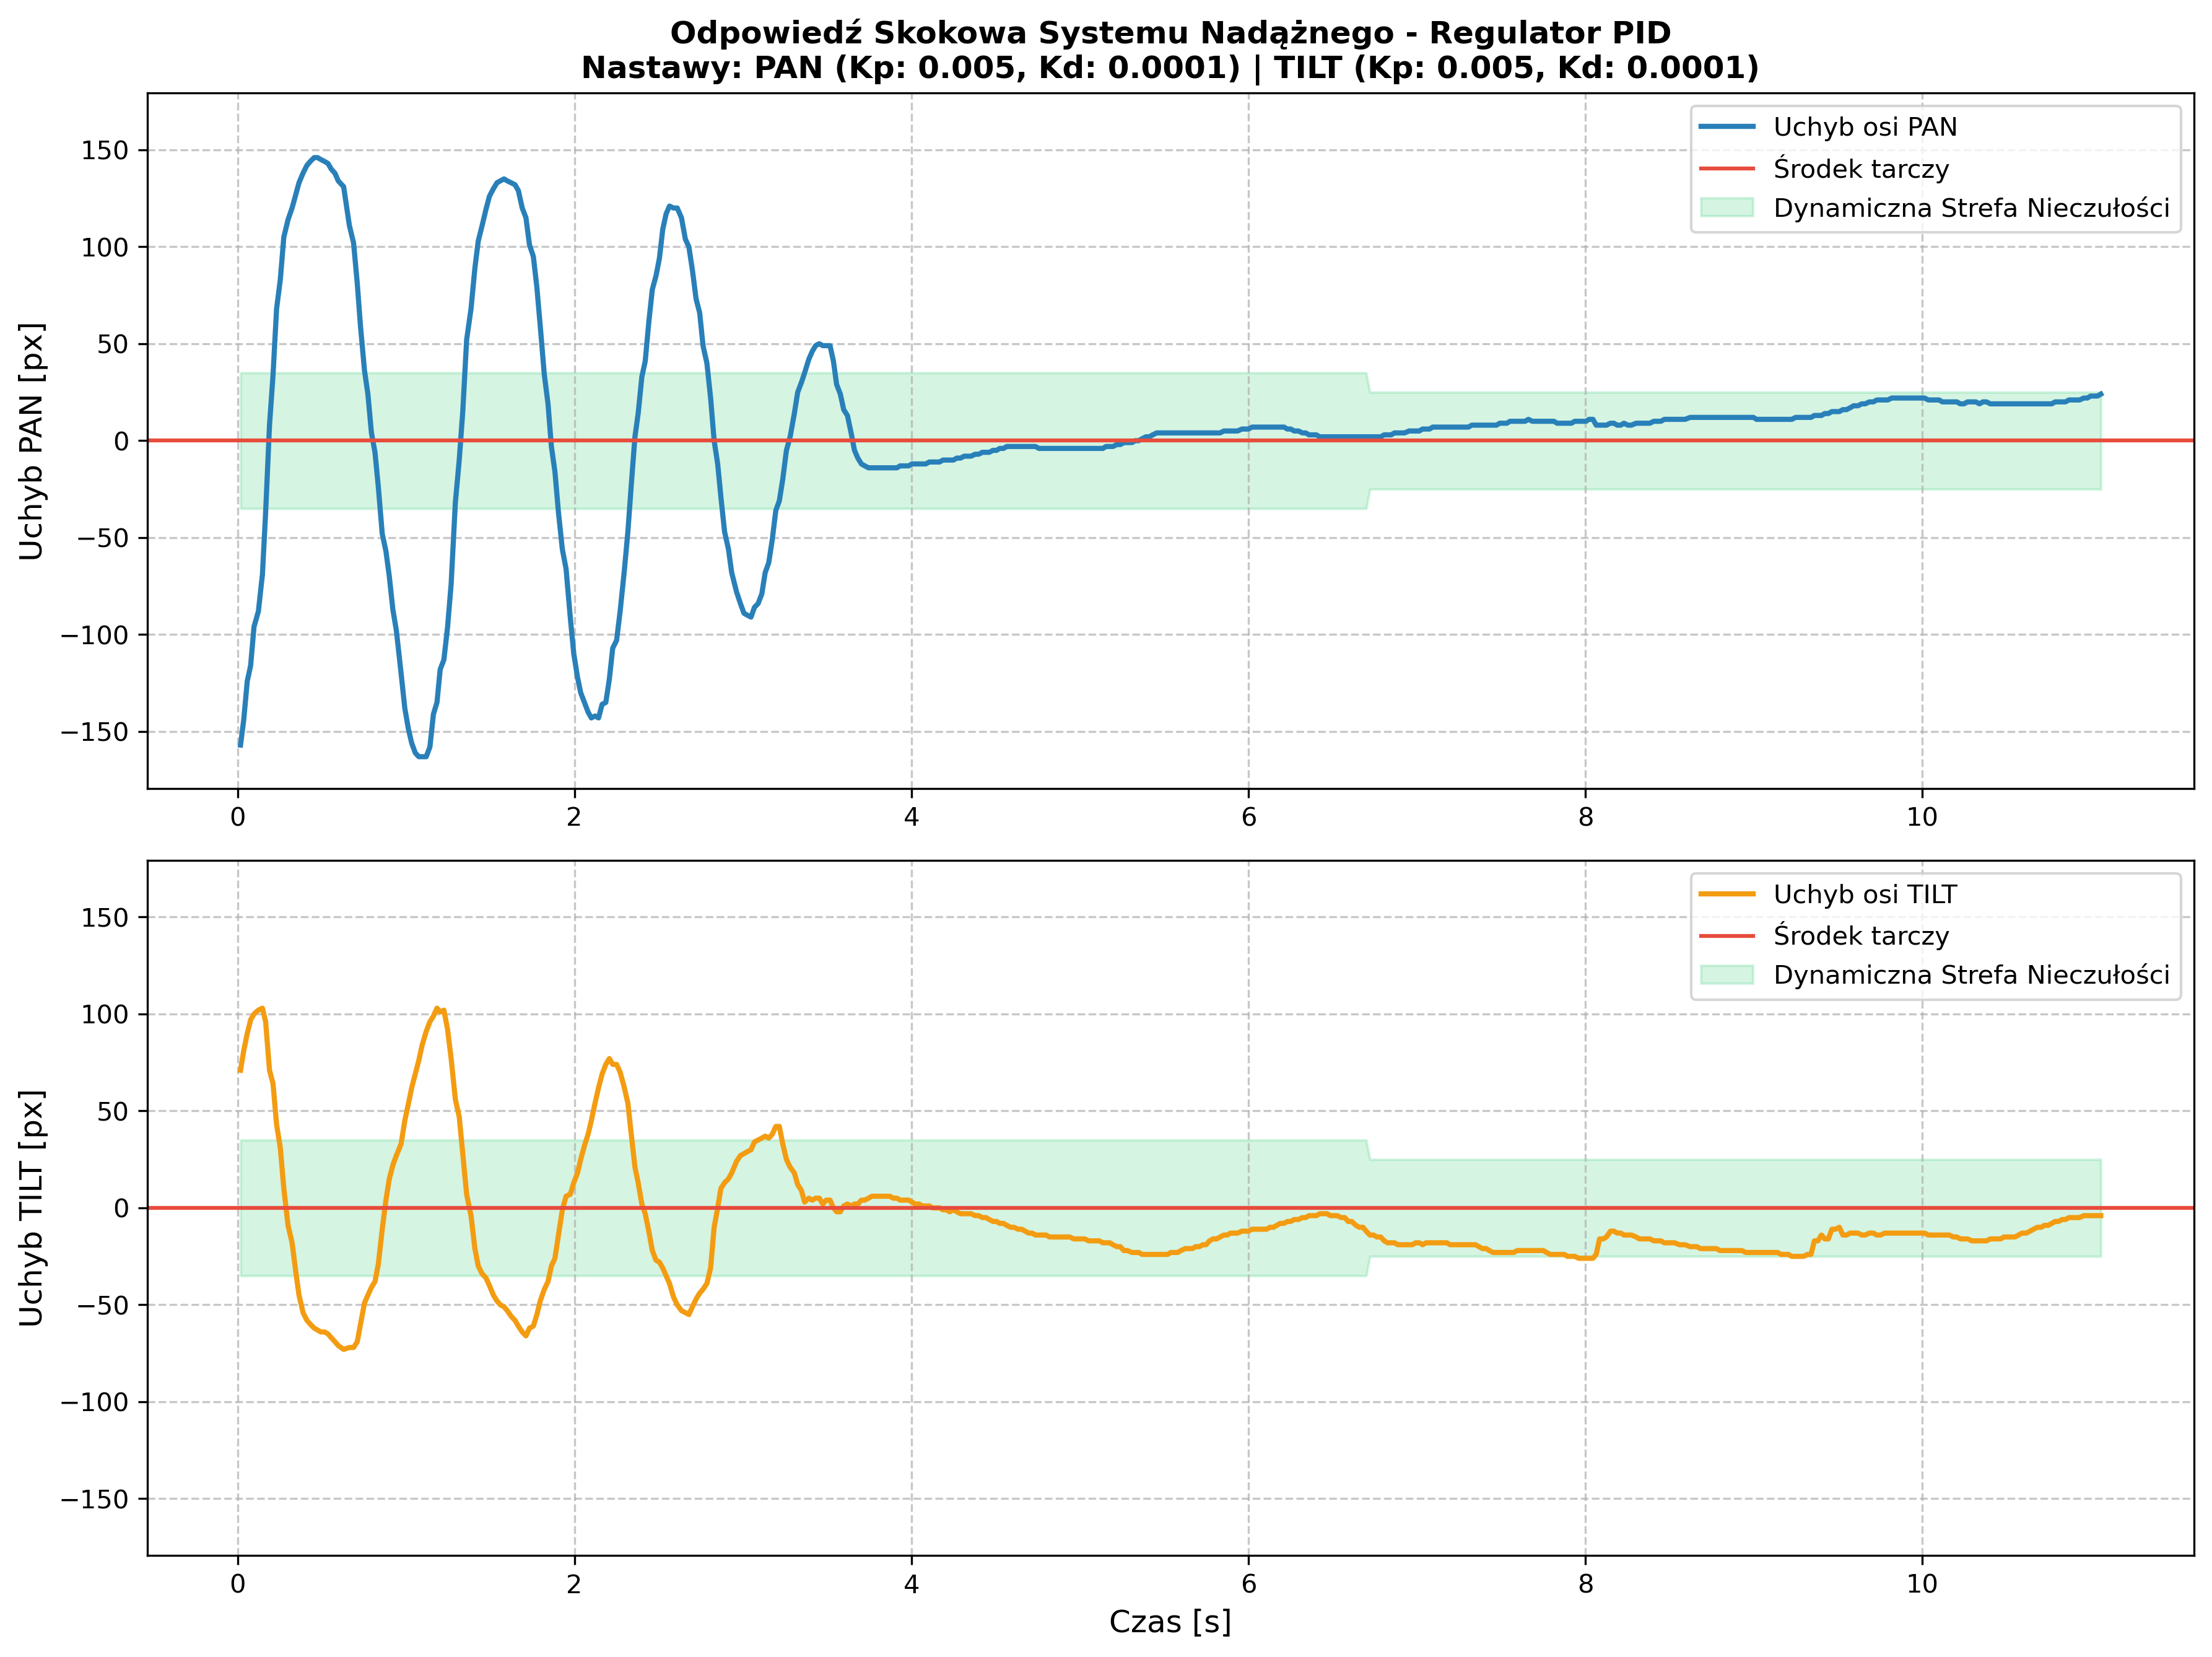
\includegraphics[width=\textwidth]{./Obrazy/Wyniki PID/wykres_GOOD_PID_move_30_150.png}
    \caption{Bez adaptacji parametrów.}
\end{subfigure}
\hfill
\begin{subfigure}{0.48\textwidth}
    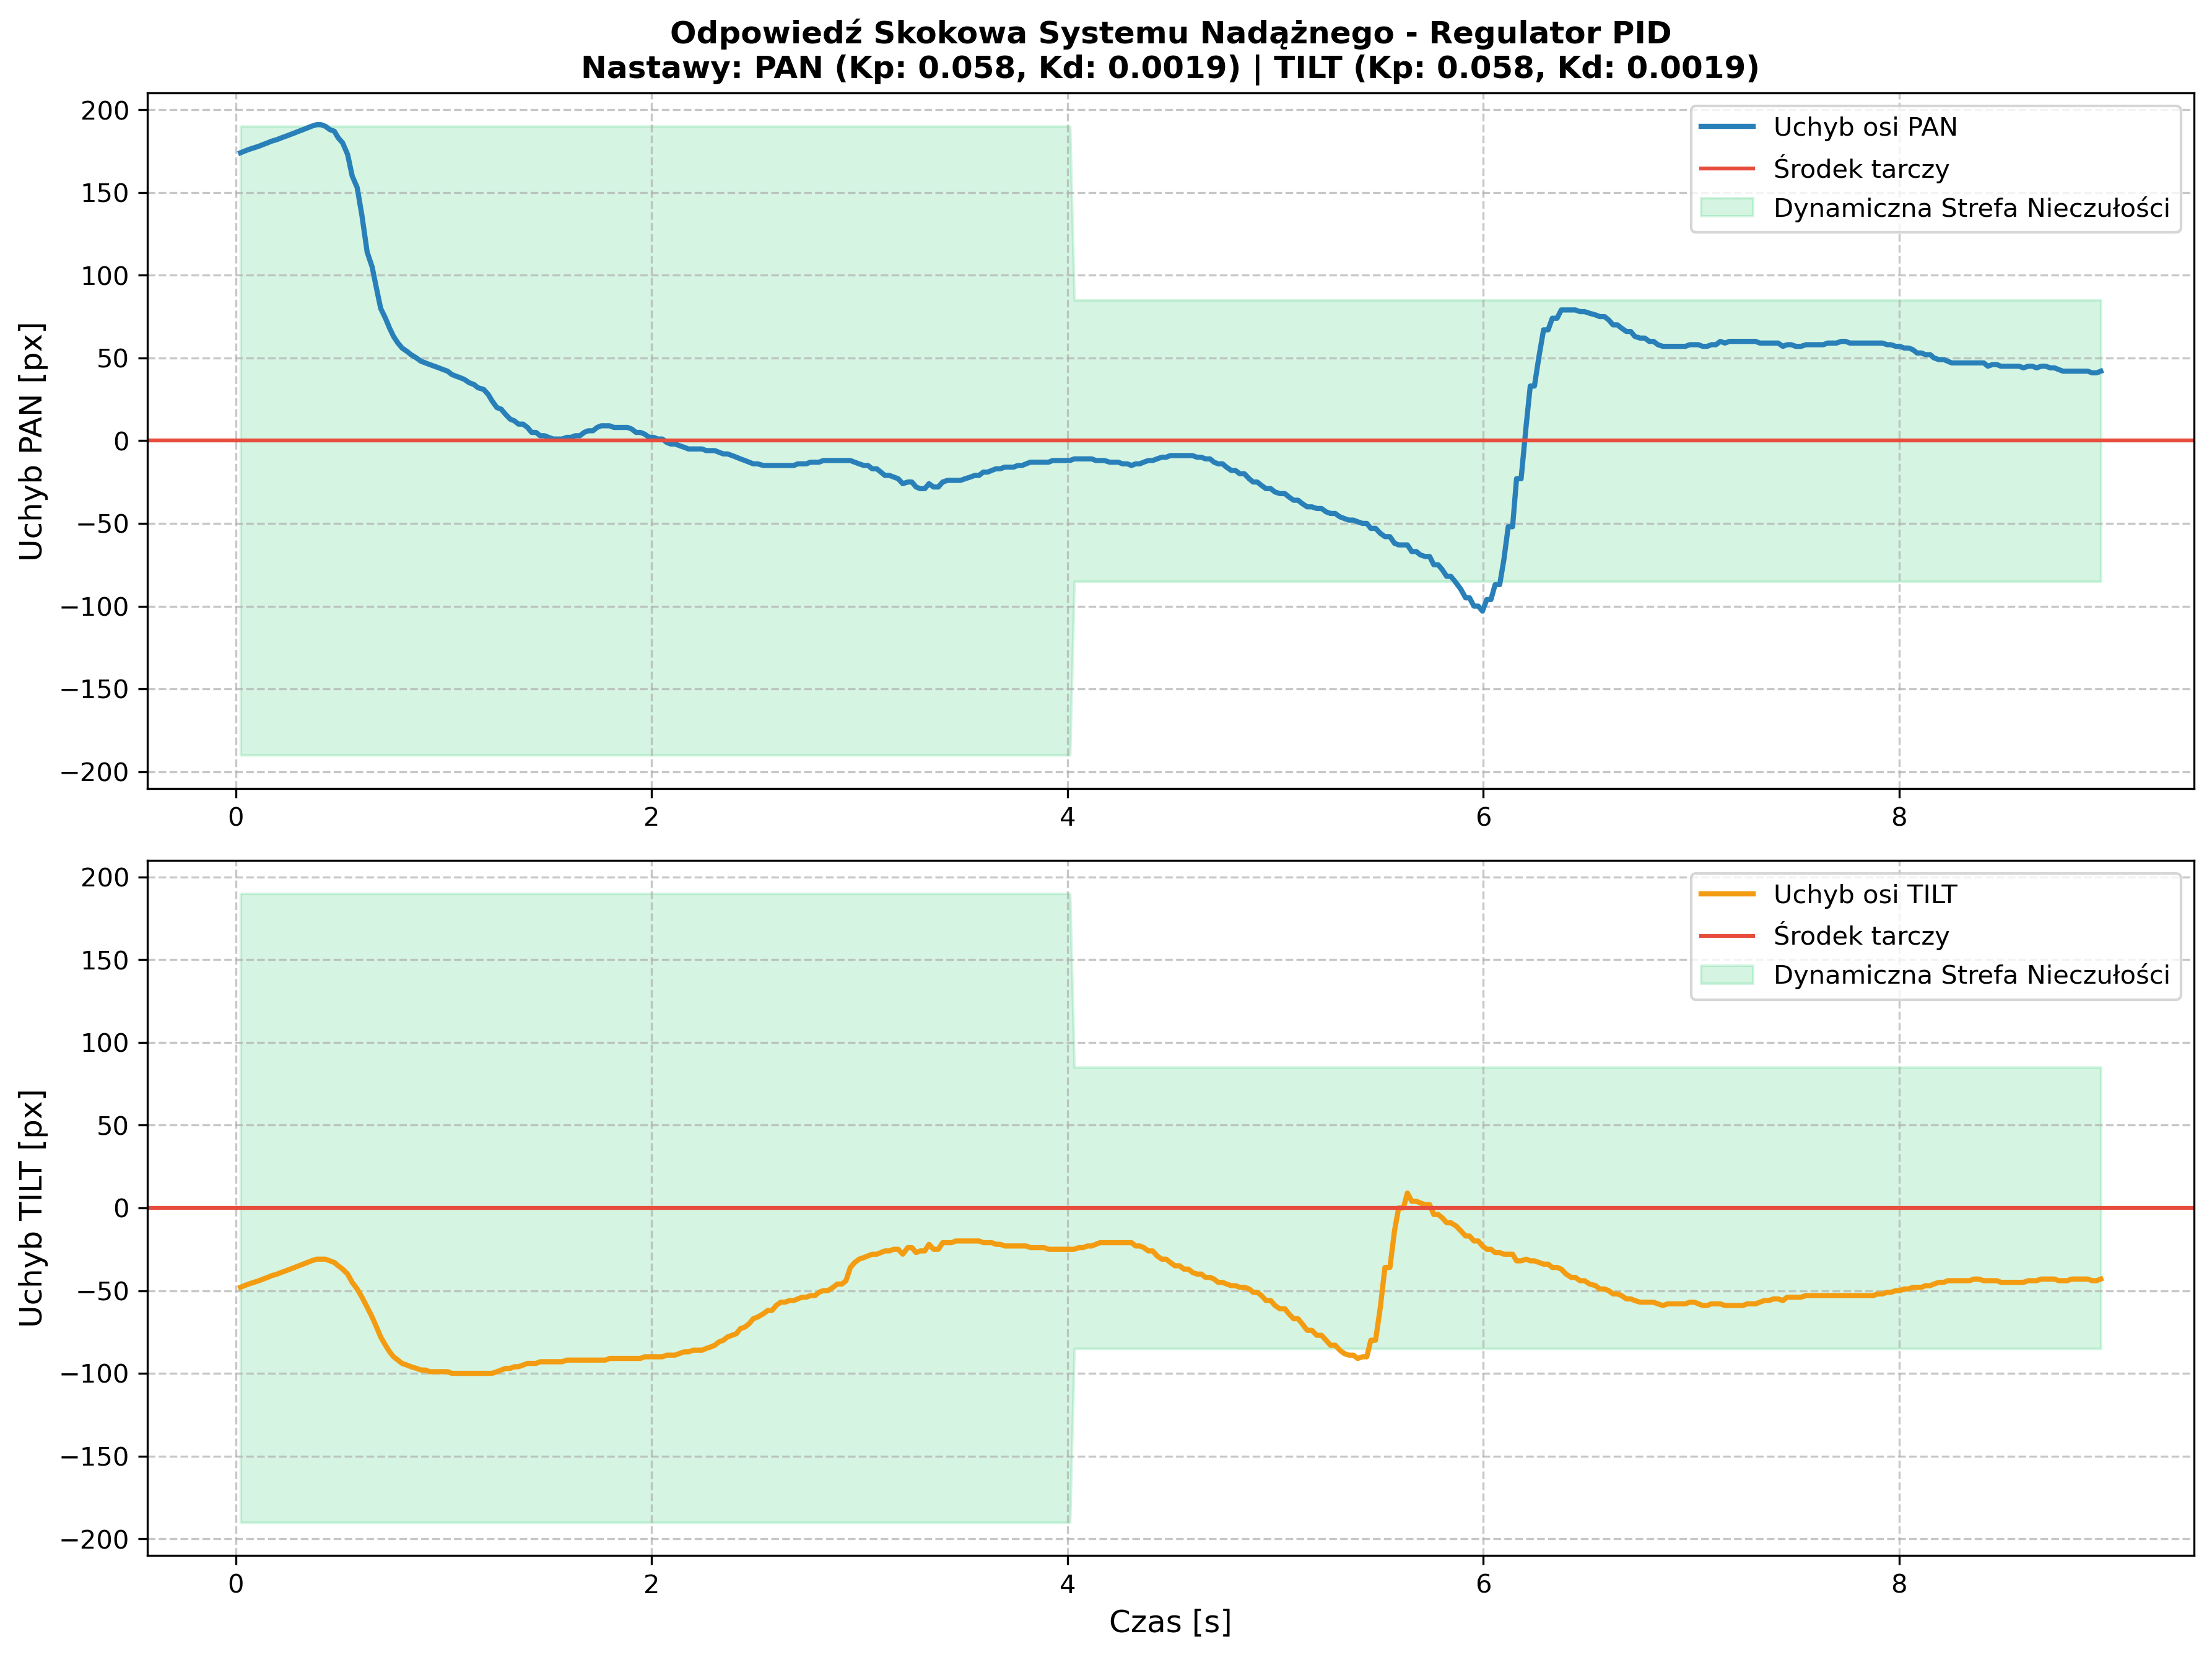
\includegraphics[width=\textwidth]{./Obrazy/Wyniki PID/wykres_UP_PID_move_30_150.png}
    \caption{Aktywny Gain Scheduling.}
\end{subfigure}
\caption{Płynne oddalanie obiektu od 30~cm do 150~cm (PID).}
\label{fig:pid_oddalanie}
\end{figure}

% =========================================================
% =========================================================
\section{Analiza działania regulatora trójpołożeniowego}
\label{sec:badania_bangbang}

Analogicznie do badań układu o działaniu ciągłym, algorytm przekaźnikowy poddano ewaluacji w identycznych scenariuszach. Porównano zachowanie przy zastosowaniu strefy nieczułości dobranej heurystycznie oraz zoptymalizowanej analitycznie na podstawie wyliczonego nadbiegu obiektu.

\subsection{Odpowiedź układu na skokową zmianę położenia celu (Ruch boczny)}
\label{subsec:bb_skok}

Zestawienie wyników na dystansie 80 cm (rys. \ref{fig:bb_skok_80}) jednoznacznie ukazuje mechanikę powstawania drgań przekaźnikowych w układach inercyjnych. Zastosowanie wąskiej, dobranej heurystycznie strefy nieczułości skutkuje tym, że wyłączony układ siłą bezwładności opuszcza obszar tolerancji z przeciwnej strony. Algorytm w odpowiedzi gwałtownie zmienia kierunek wysterowania, wprowadzając wieżyczkę w permanentny cykl limitowy. Wdrożenie strefy wyznaczonej analitycznie, poszerzonej o wyliczoną wcześniej drogę hamowania, pozwoliło na pewne wejście uchybu w obszar tolerancji i trwałe wyłączenie napędów, potwierdzając słuszność wyliczeń z rozdziału 5.

\begin{figure}[!ht]
\centering
\begin{subfigure}{0.48\textwidth}
    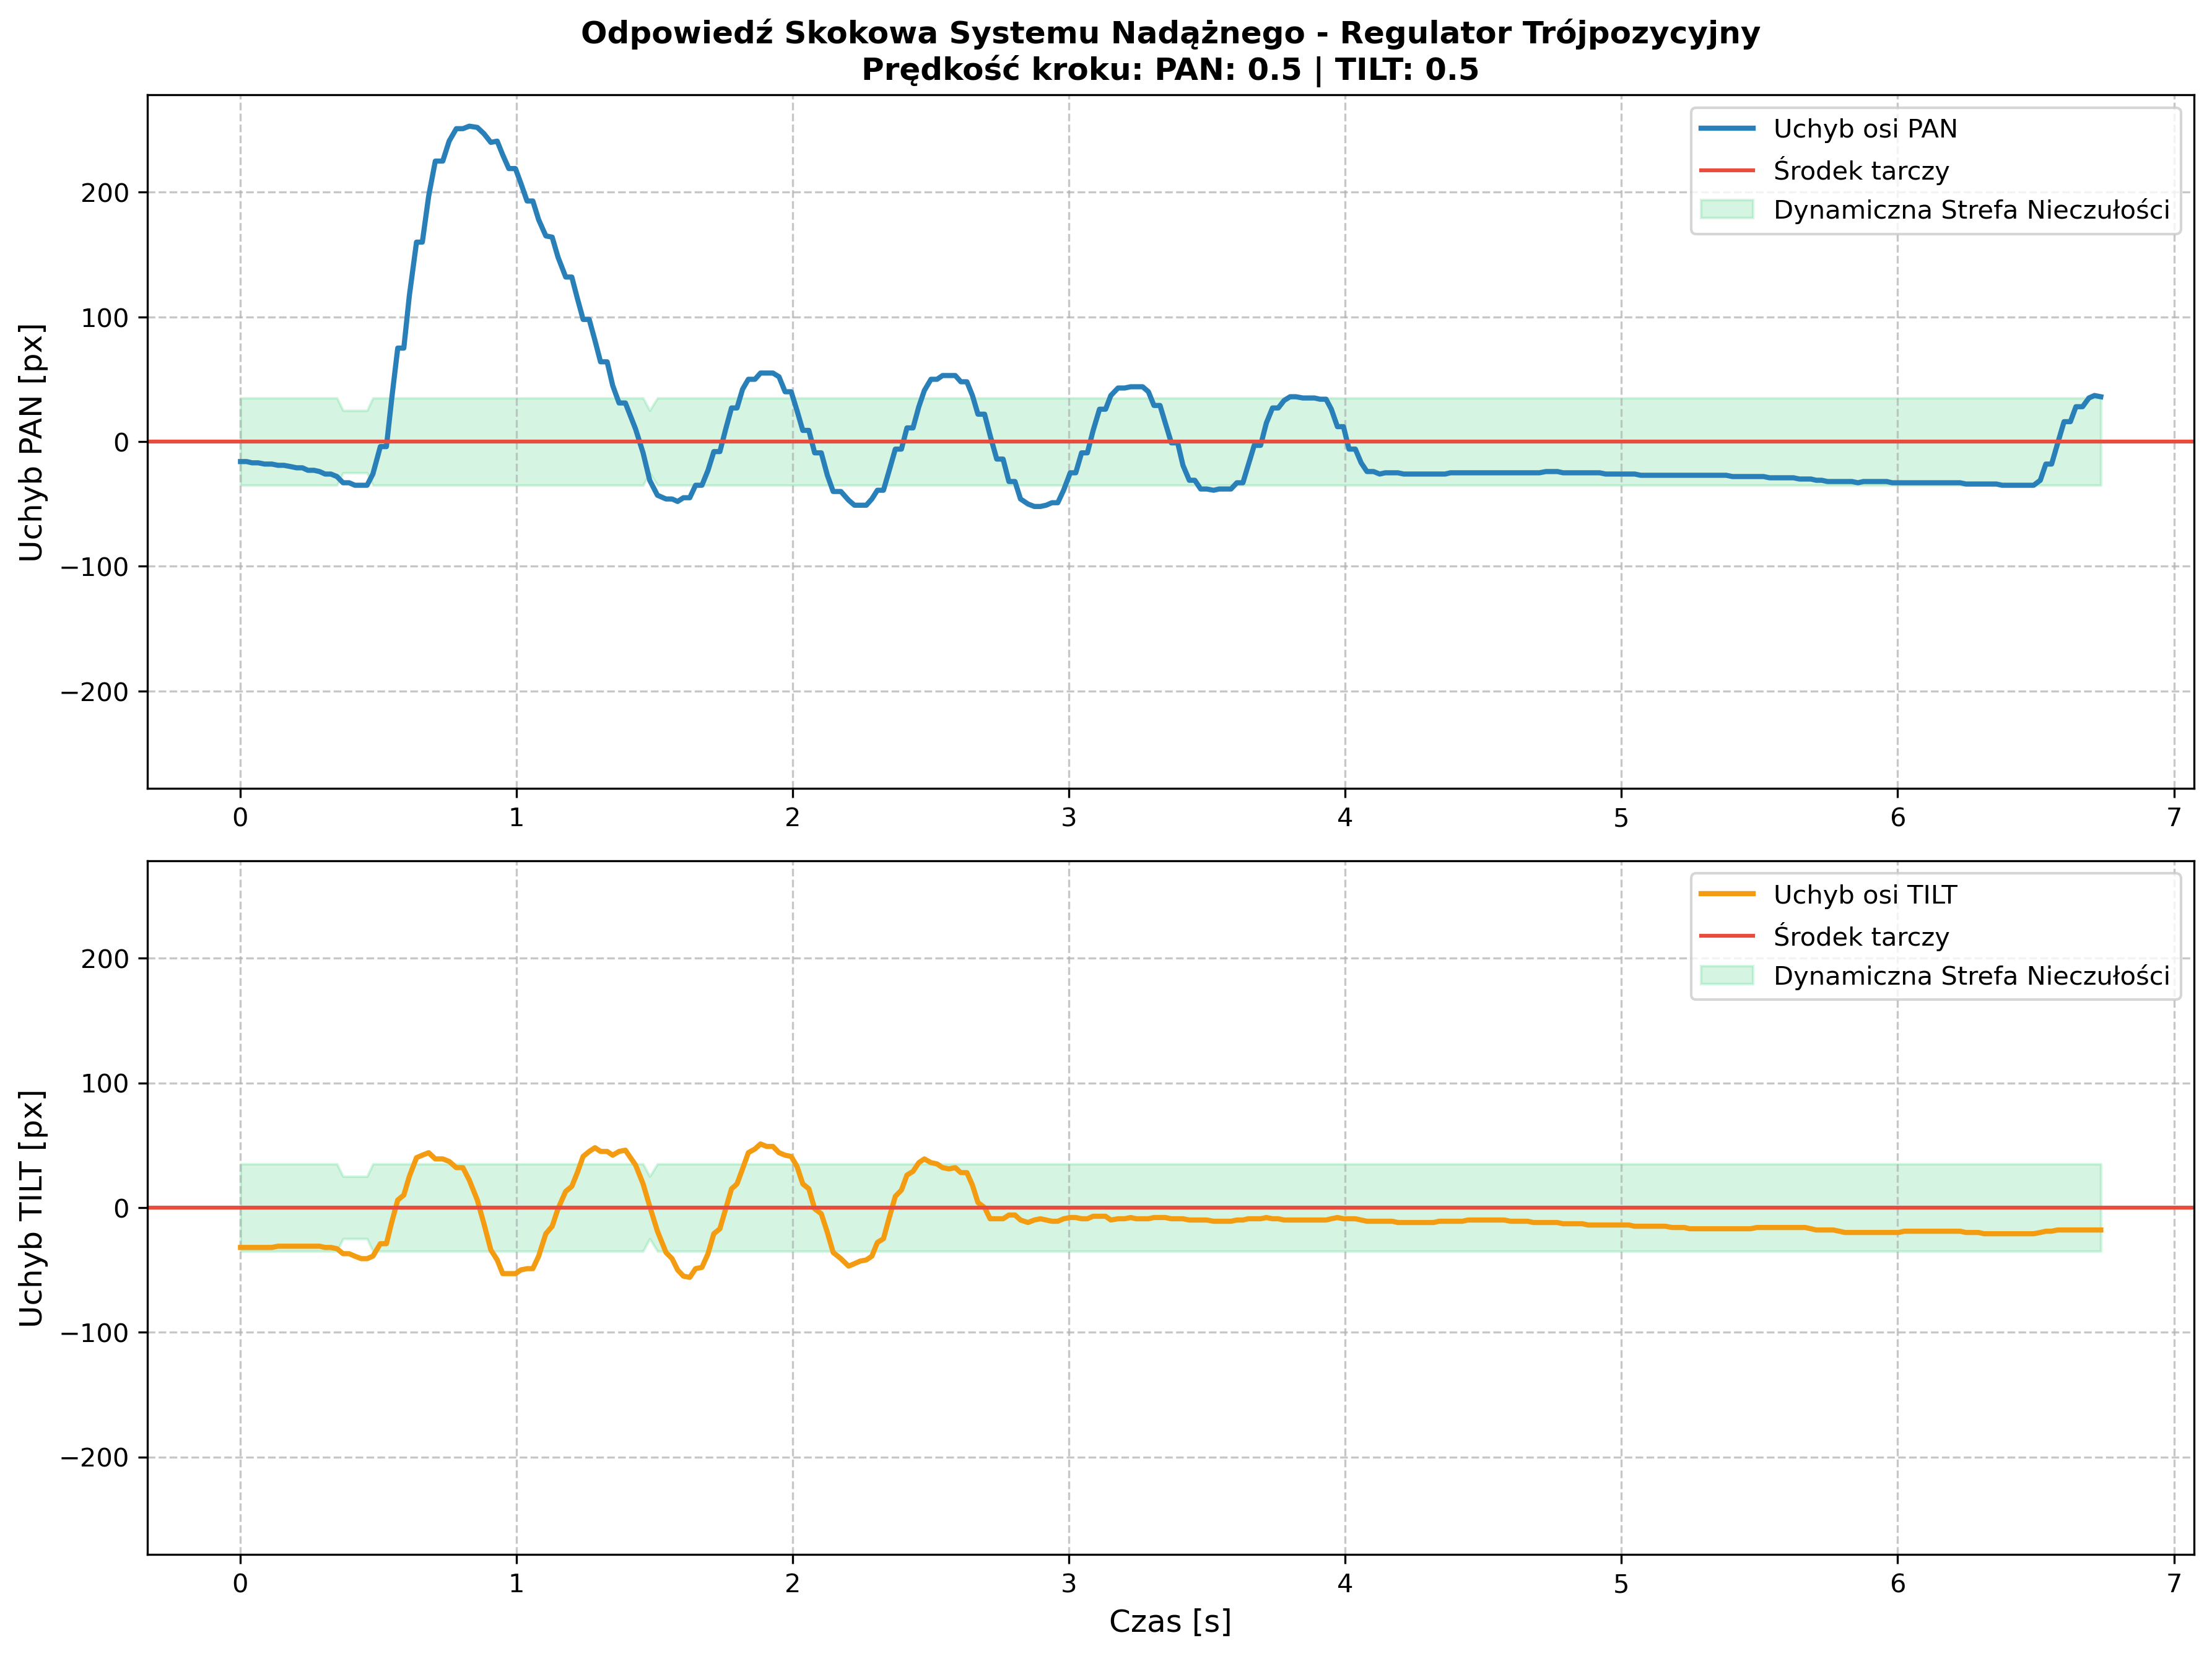
\includegraphics[width=\textwidth]{./Obrazy/WYniki troj/wykres_GOOD_BB_move_80_cm.png}
    \caption{Strefa heurystyczna.}
\end{subfigure}
\hfill
\begin{subfigure}{0.48\textwidth}
    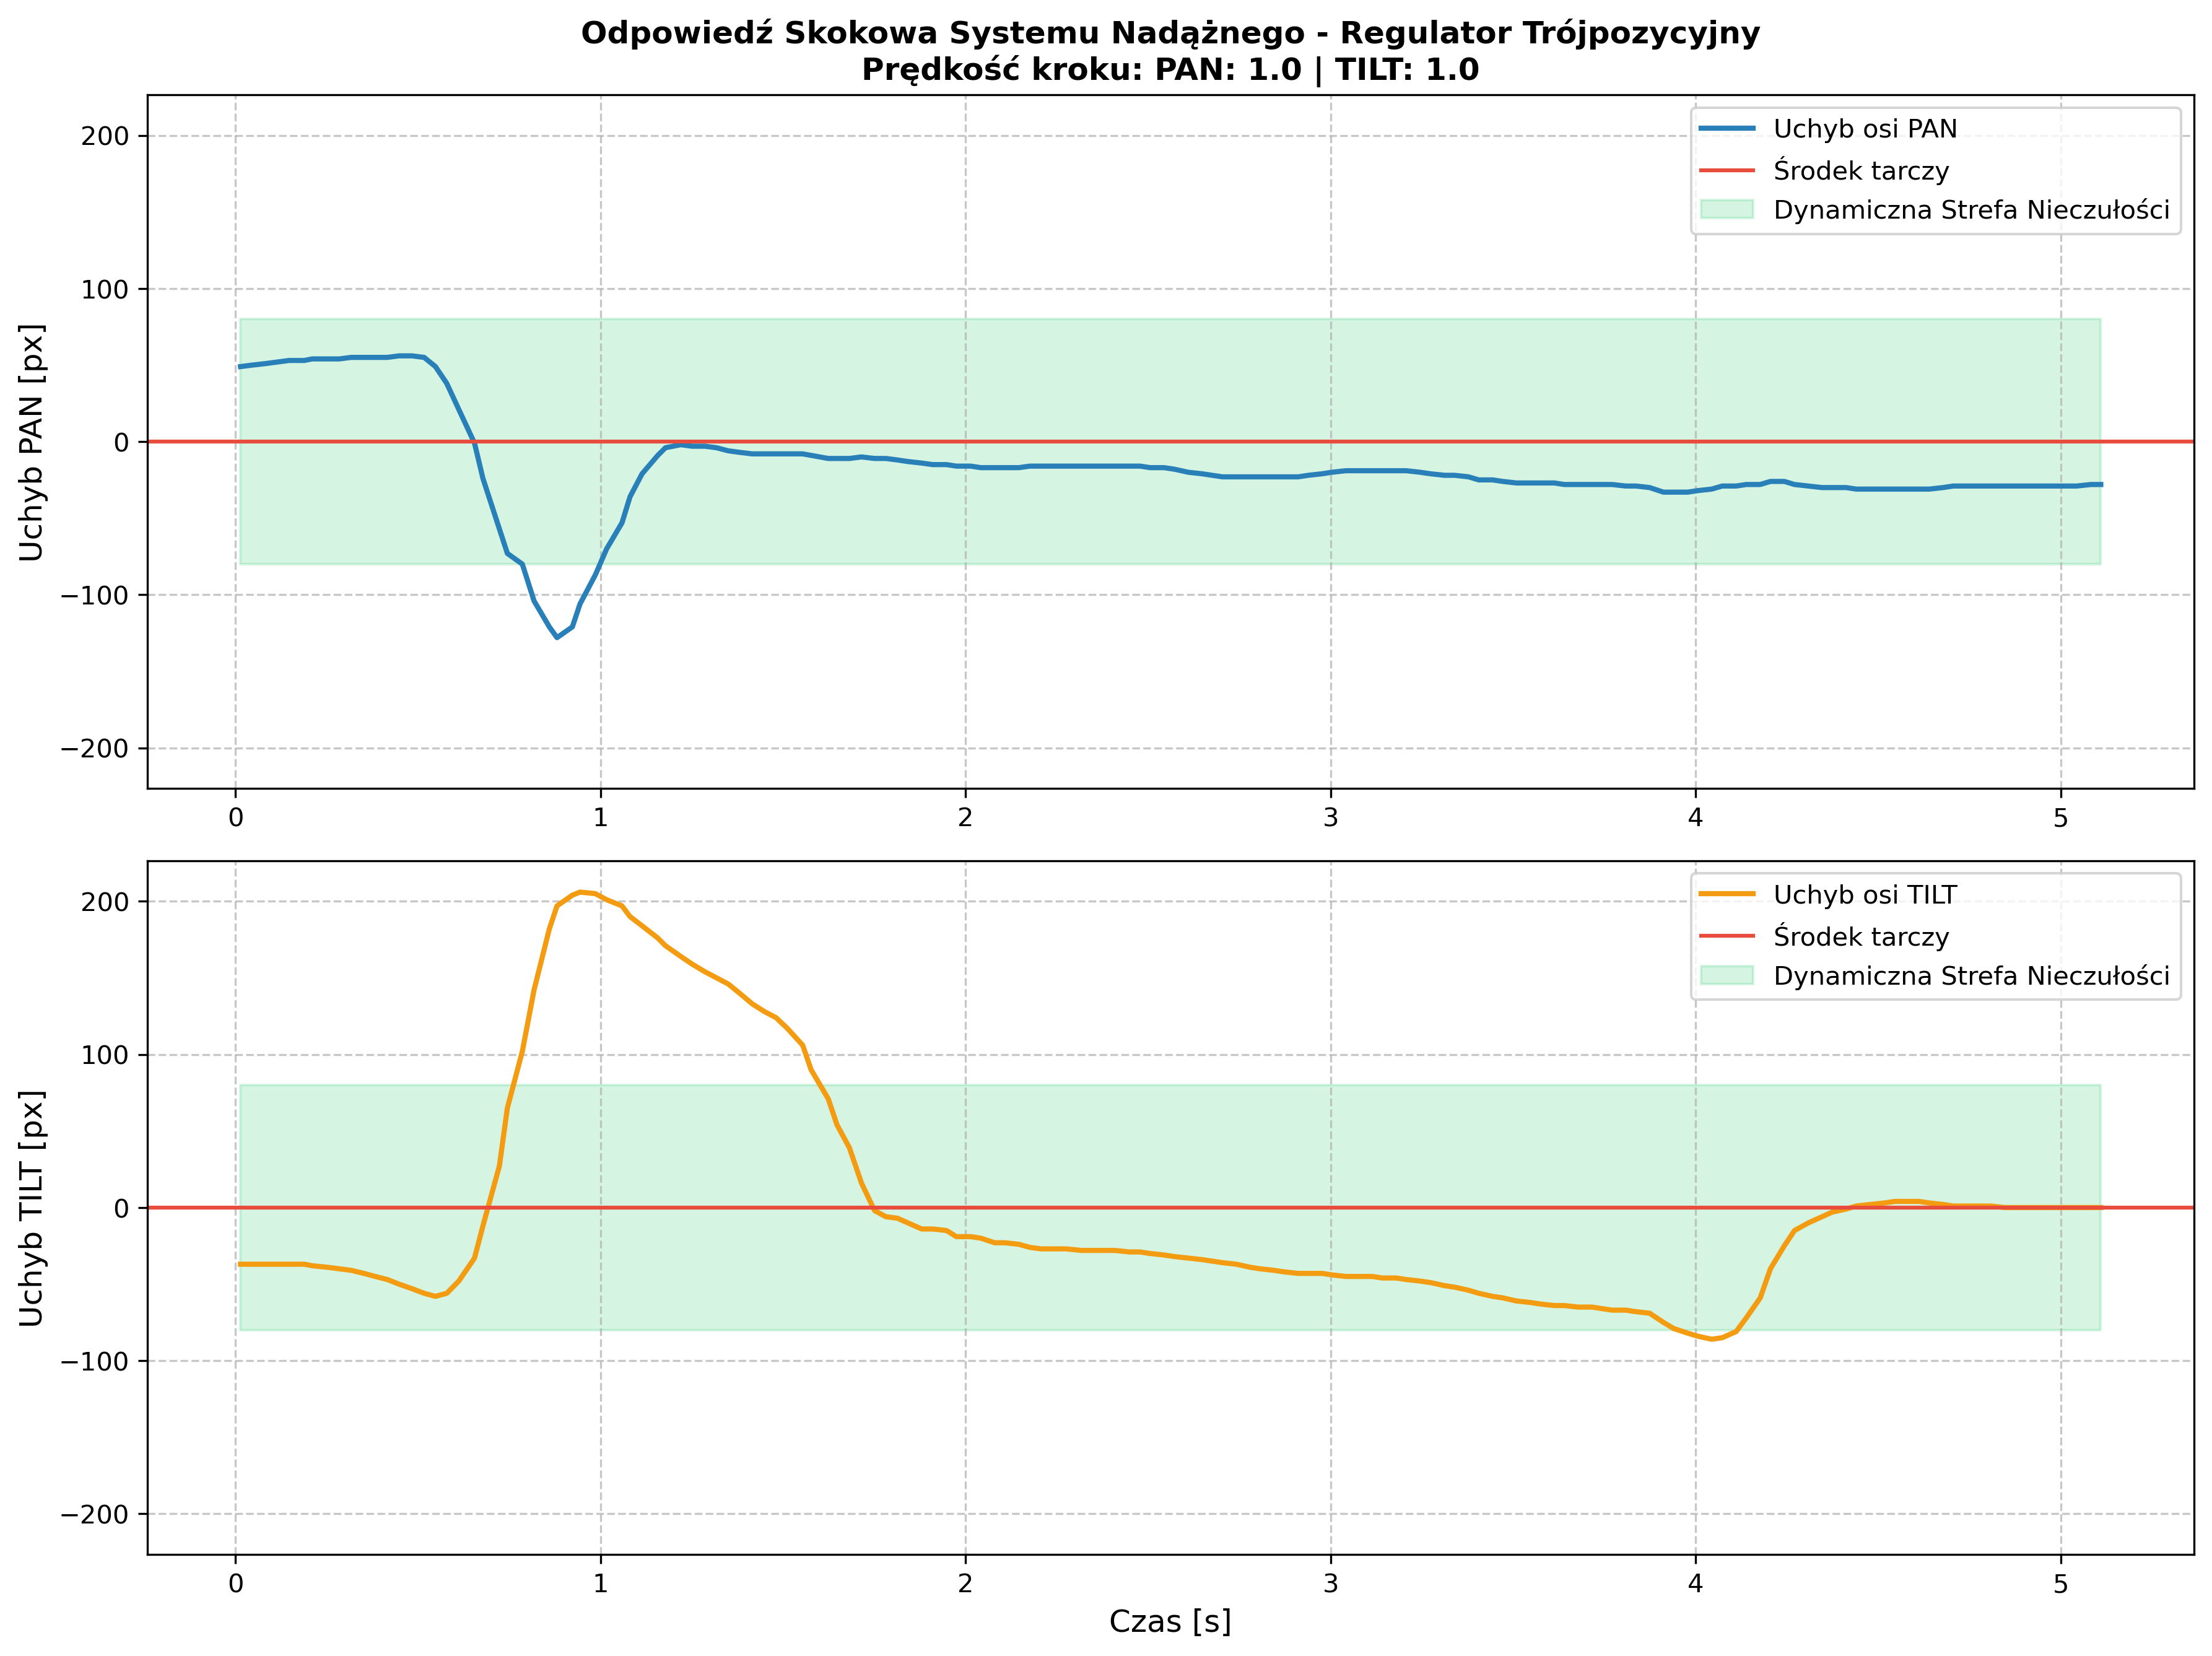
\includegraphics[width=\textwidth]{./Obrazy/WYniki troj/wykres_UP_BB_move_80_cm.png}
    \caption{Strefa analityczna.}
\end{subfigure}
\caption{Porównanie odpowiedzi skokowej regulatora trójpołożeniowego na dystansie 80~cm.}
\label{fig:bb_skok_80}
\end{figure}

Skrócenie dystansu do 30 cm (rys. \ref{fig:bb_skok_30}) drastycznie uwypukliło problemy niestrojonego algorytmu Bang-Bang. Z powodu ogromnej prędkości pozornej celu, amplituda drgań dla nastaw heurystycznych wzrosła do wartości niemal 300 pikseli, co w praktyce oznaczało całkowitą utratę zdolności śledzenia i gwałtowne "rzucanie" całą konstrukcją wieżyczki. Zastosowanie nastaw analitycznych, wspartych systemem adaptacyjnym poszerzającym strefę nieczułości dla obiektów bliskich, pozwoliło opanować układ. Zwiększona prędkość osi PAN błyskawicznie zniwelowała początkowy błąd, a szeroki bufor bezpieczeństwa "wchłonął" energię kinetyczną hamowania.

\begin{figure}[!ht]
\centering
\begin{subfigure}{0.48\textwidth}
    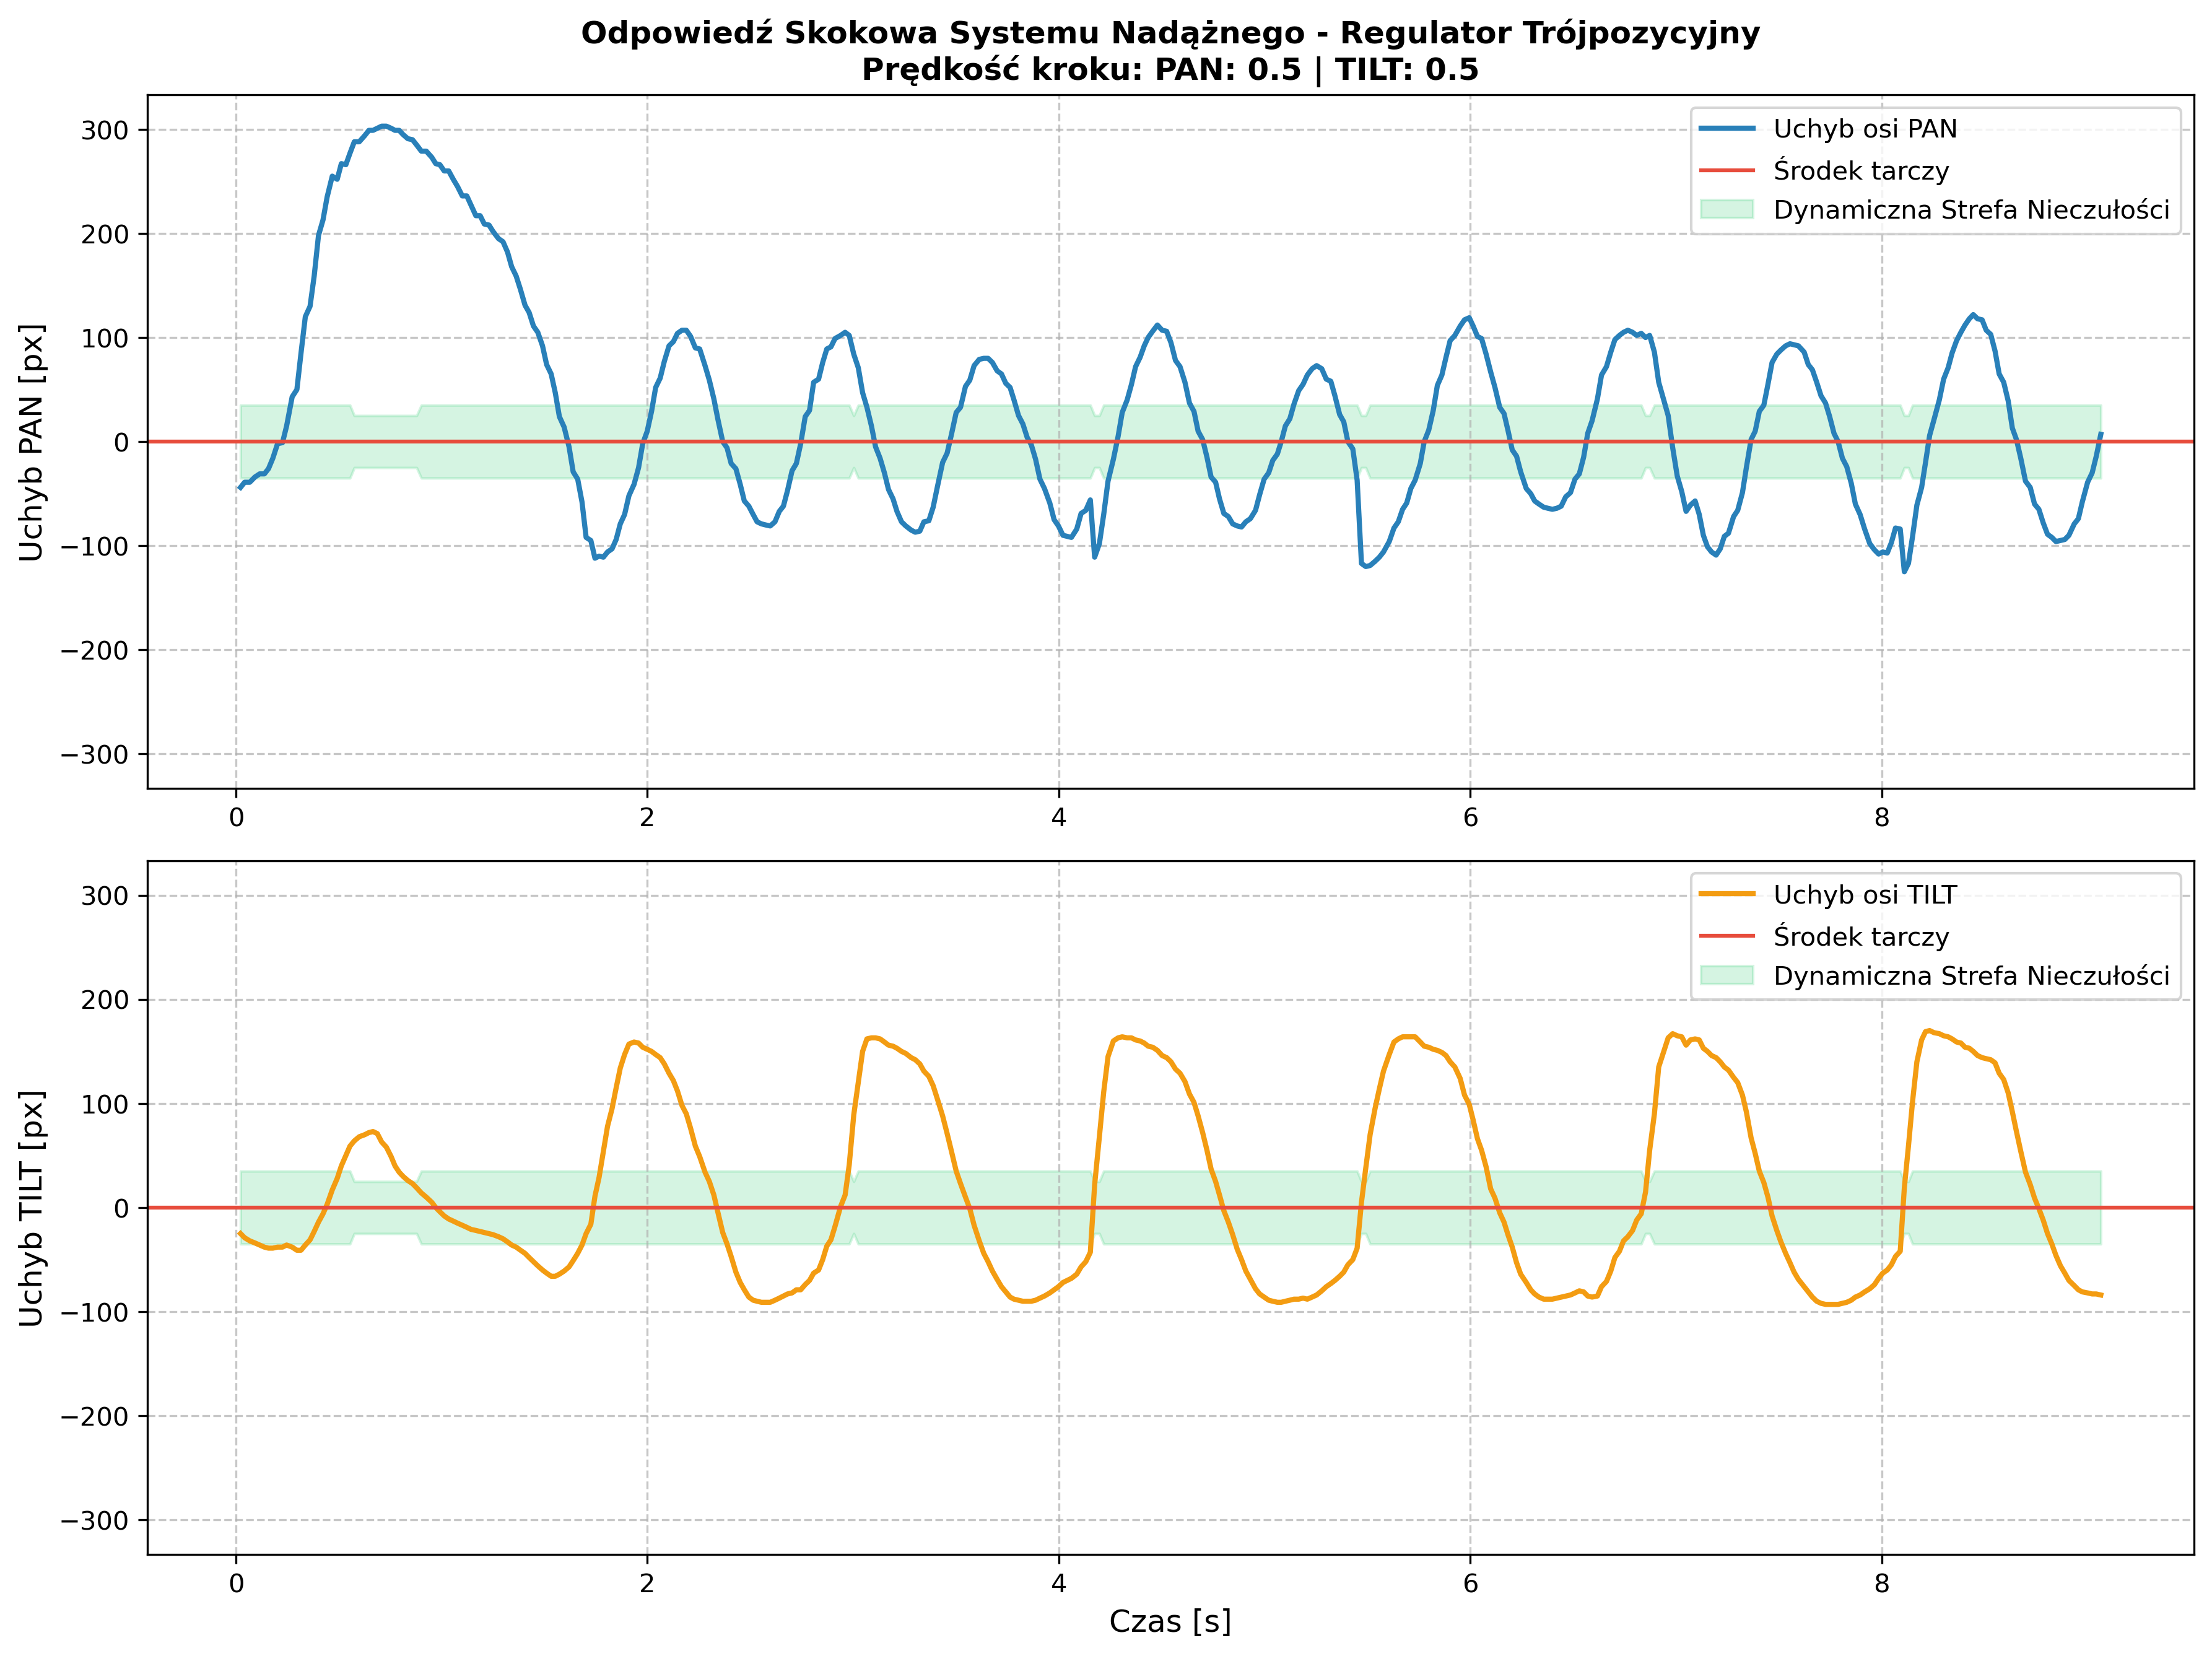
\includegraphics[width=\textwidth]{./Obrazy/WYniki troj/wykres_GOOD_BB_move_30_cm.png}
    \caption{Strefa heurystyczna.}
\end{subfigure}
\hfill
\begin{subfigure}{0.48\textwidth}
    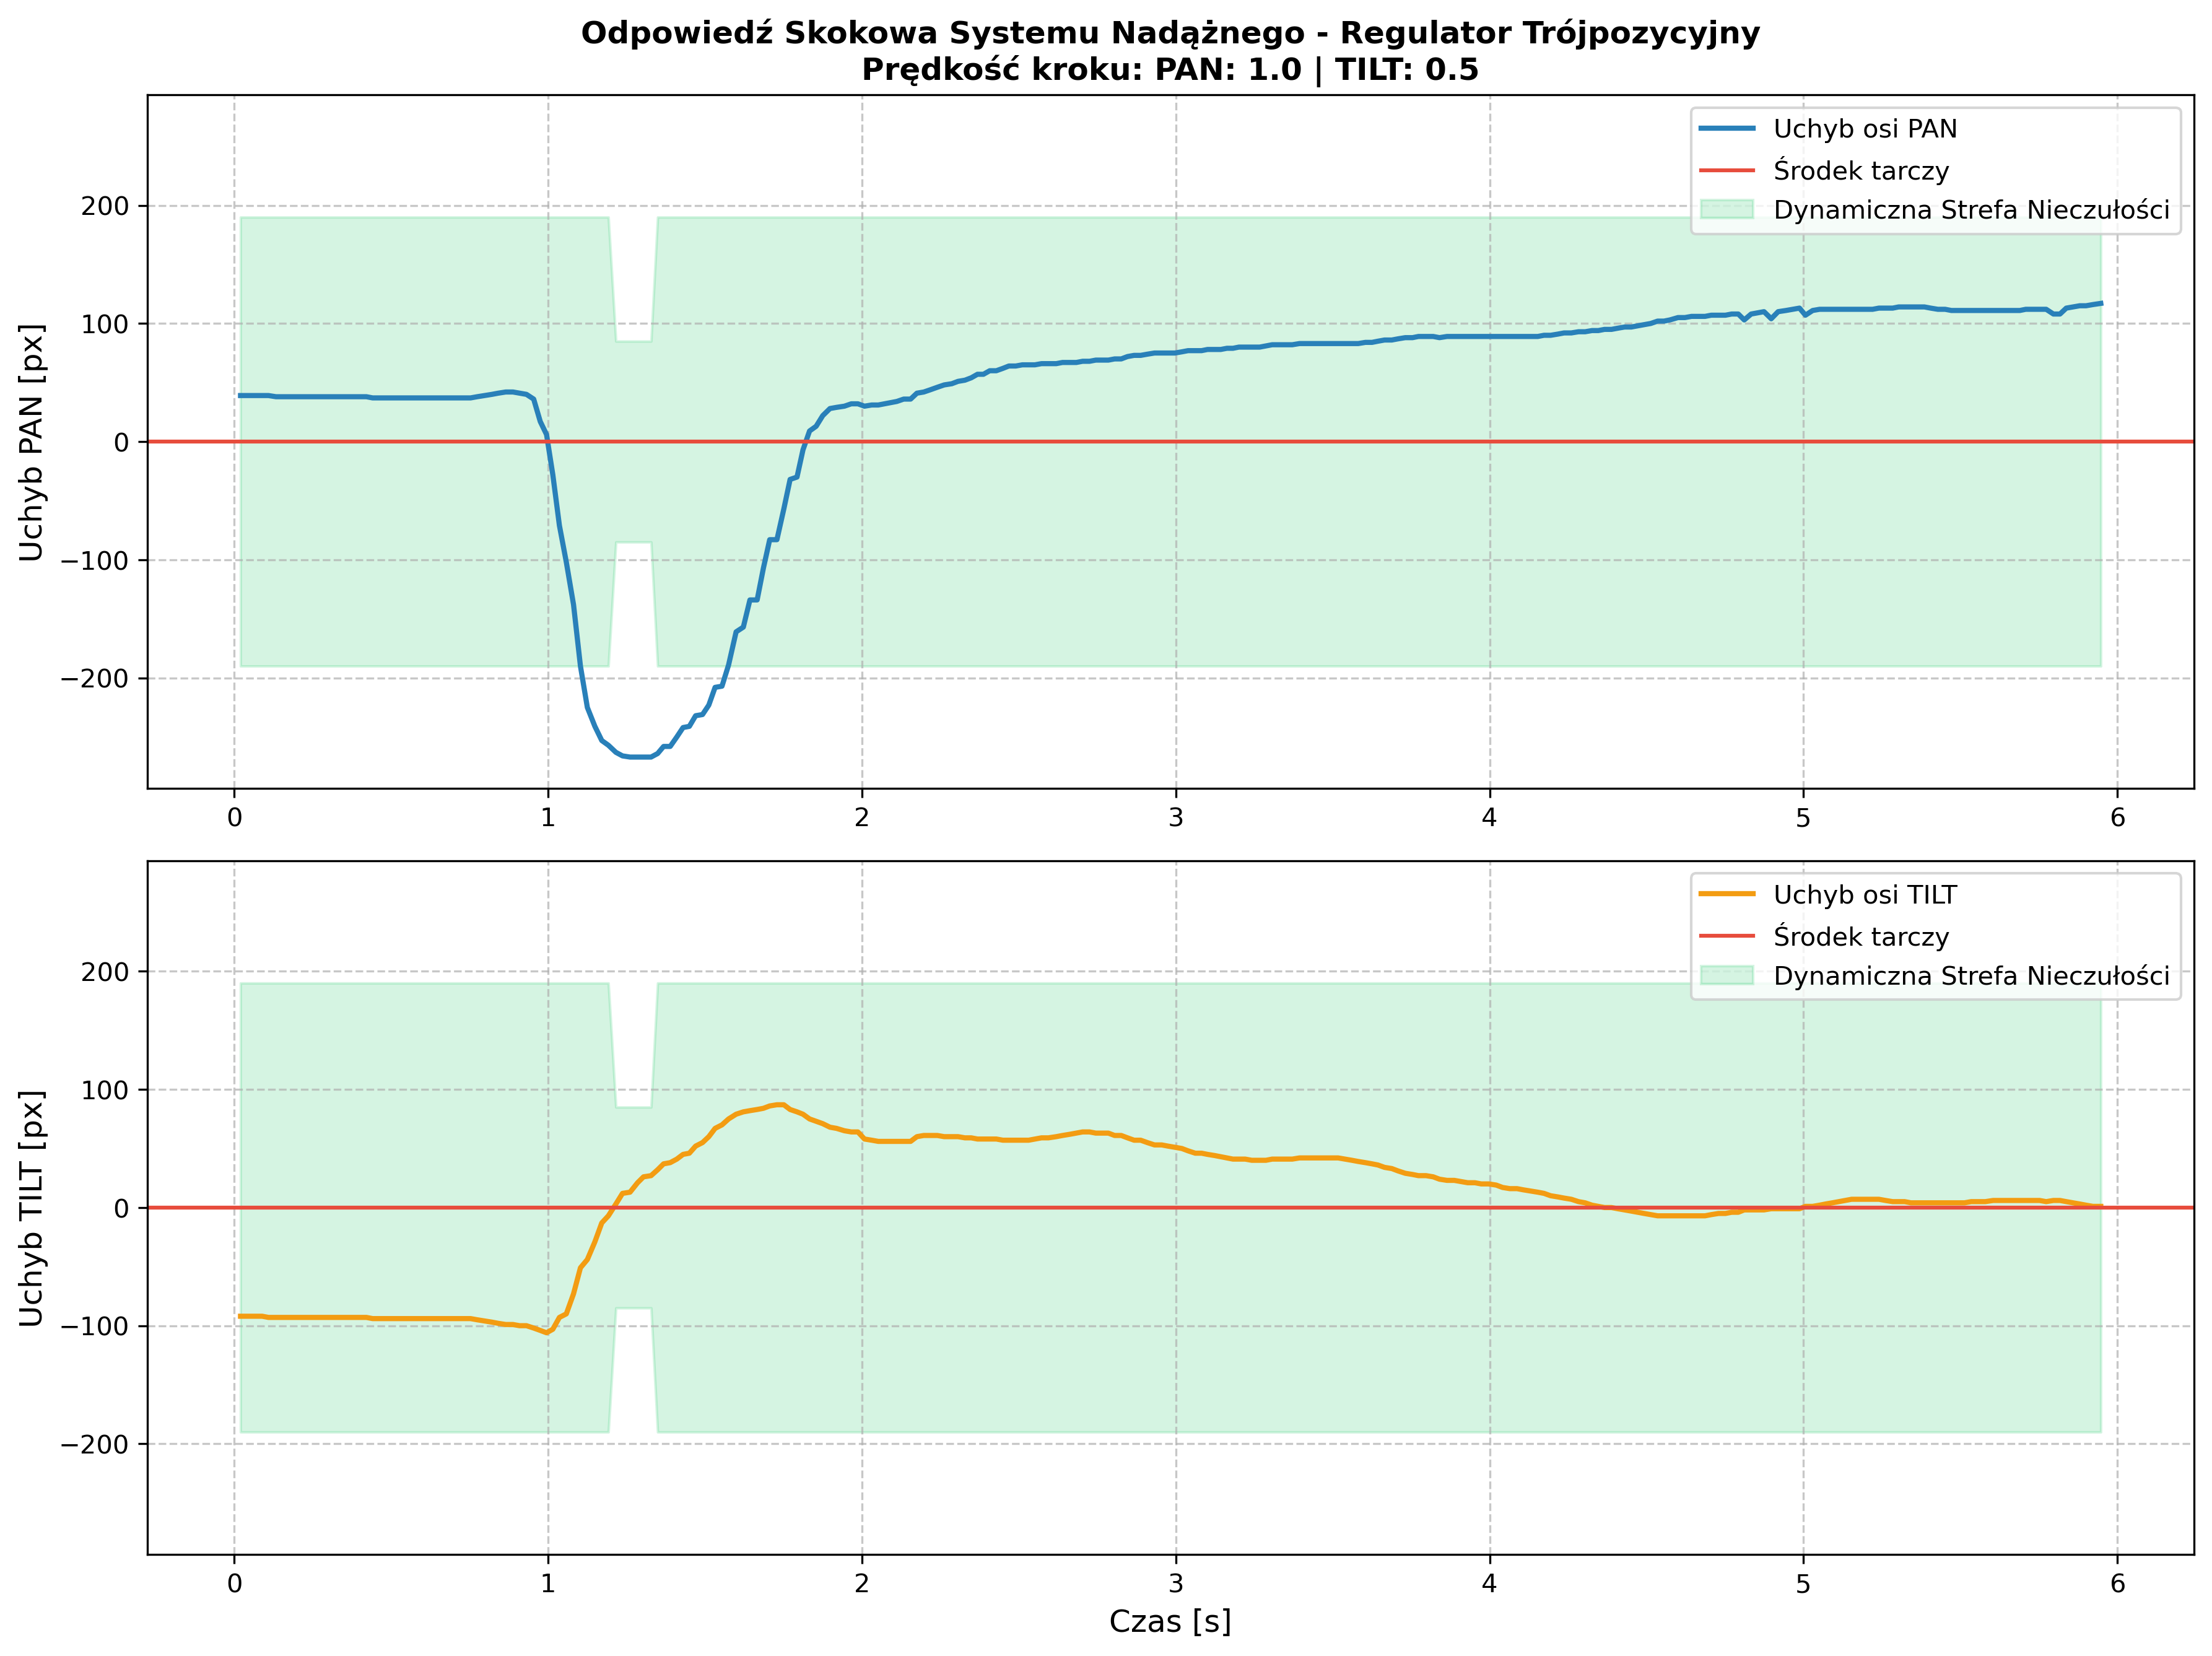
\includegraphics[width=\textwidth]{./Obrazy/WYniki troj/wykres_UP_BB_move_30_cm.png}
    \caption{Strefa analityczna.}
\end{subfigure}
\caption{Porównanie odpowiedzi skokowej regulatora trójpołożeniowego na dystansie 30~cm.}
\label{fig:bb_skok_30}
\end{figure}

Na dystansie 150 cm (rys. \ref{fig:bb_skok_150}), gdzie obiekt jest relatywnie mały, nastawy heurystyczne wciąż wykazywały tendencję do wzbudzania oscylacji (szczególnie widocznych w osi PAN). Podejście analityczne udowodniło swoją wyższość również w tym scenariuszu. Dzięki algorytmowi Gain Scheduling, który automatycznie zawęził strefę nieczułości po wykryciu małego pola powierzchni obiektu, układ nie tylko zachował absolutną stabilność po pierwszym hamowaniu, ale również zagwarantował zadowalającą precyzję centrowania, nie pozwalając celowi na nadmierne "pływanie" po szerokim kadrze.

\begin{figure}[!ht]
\centering
\begin{subfigure}{0.48\textwidth}
    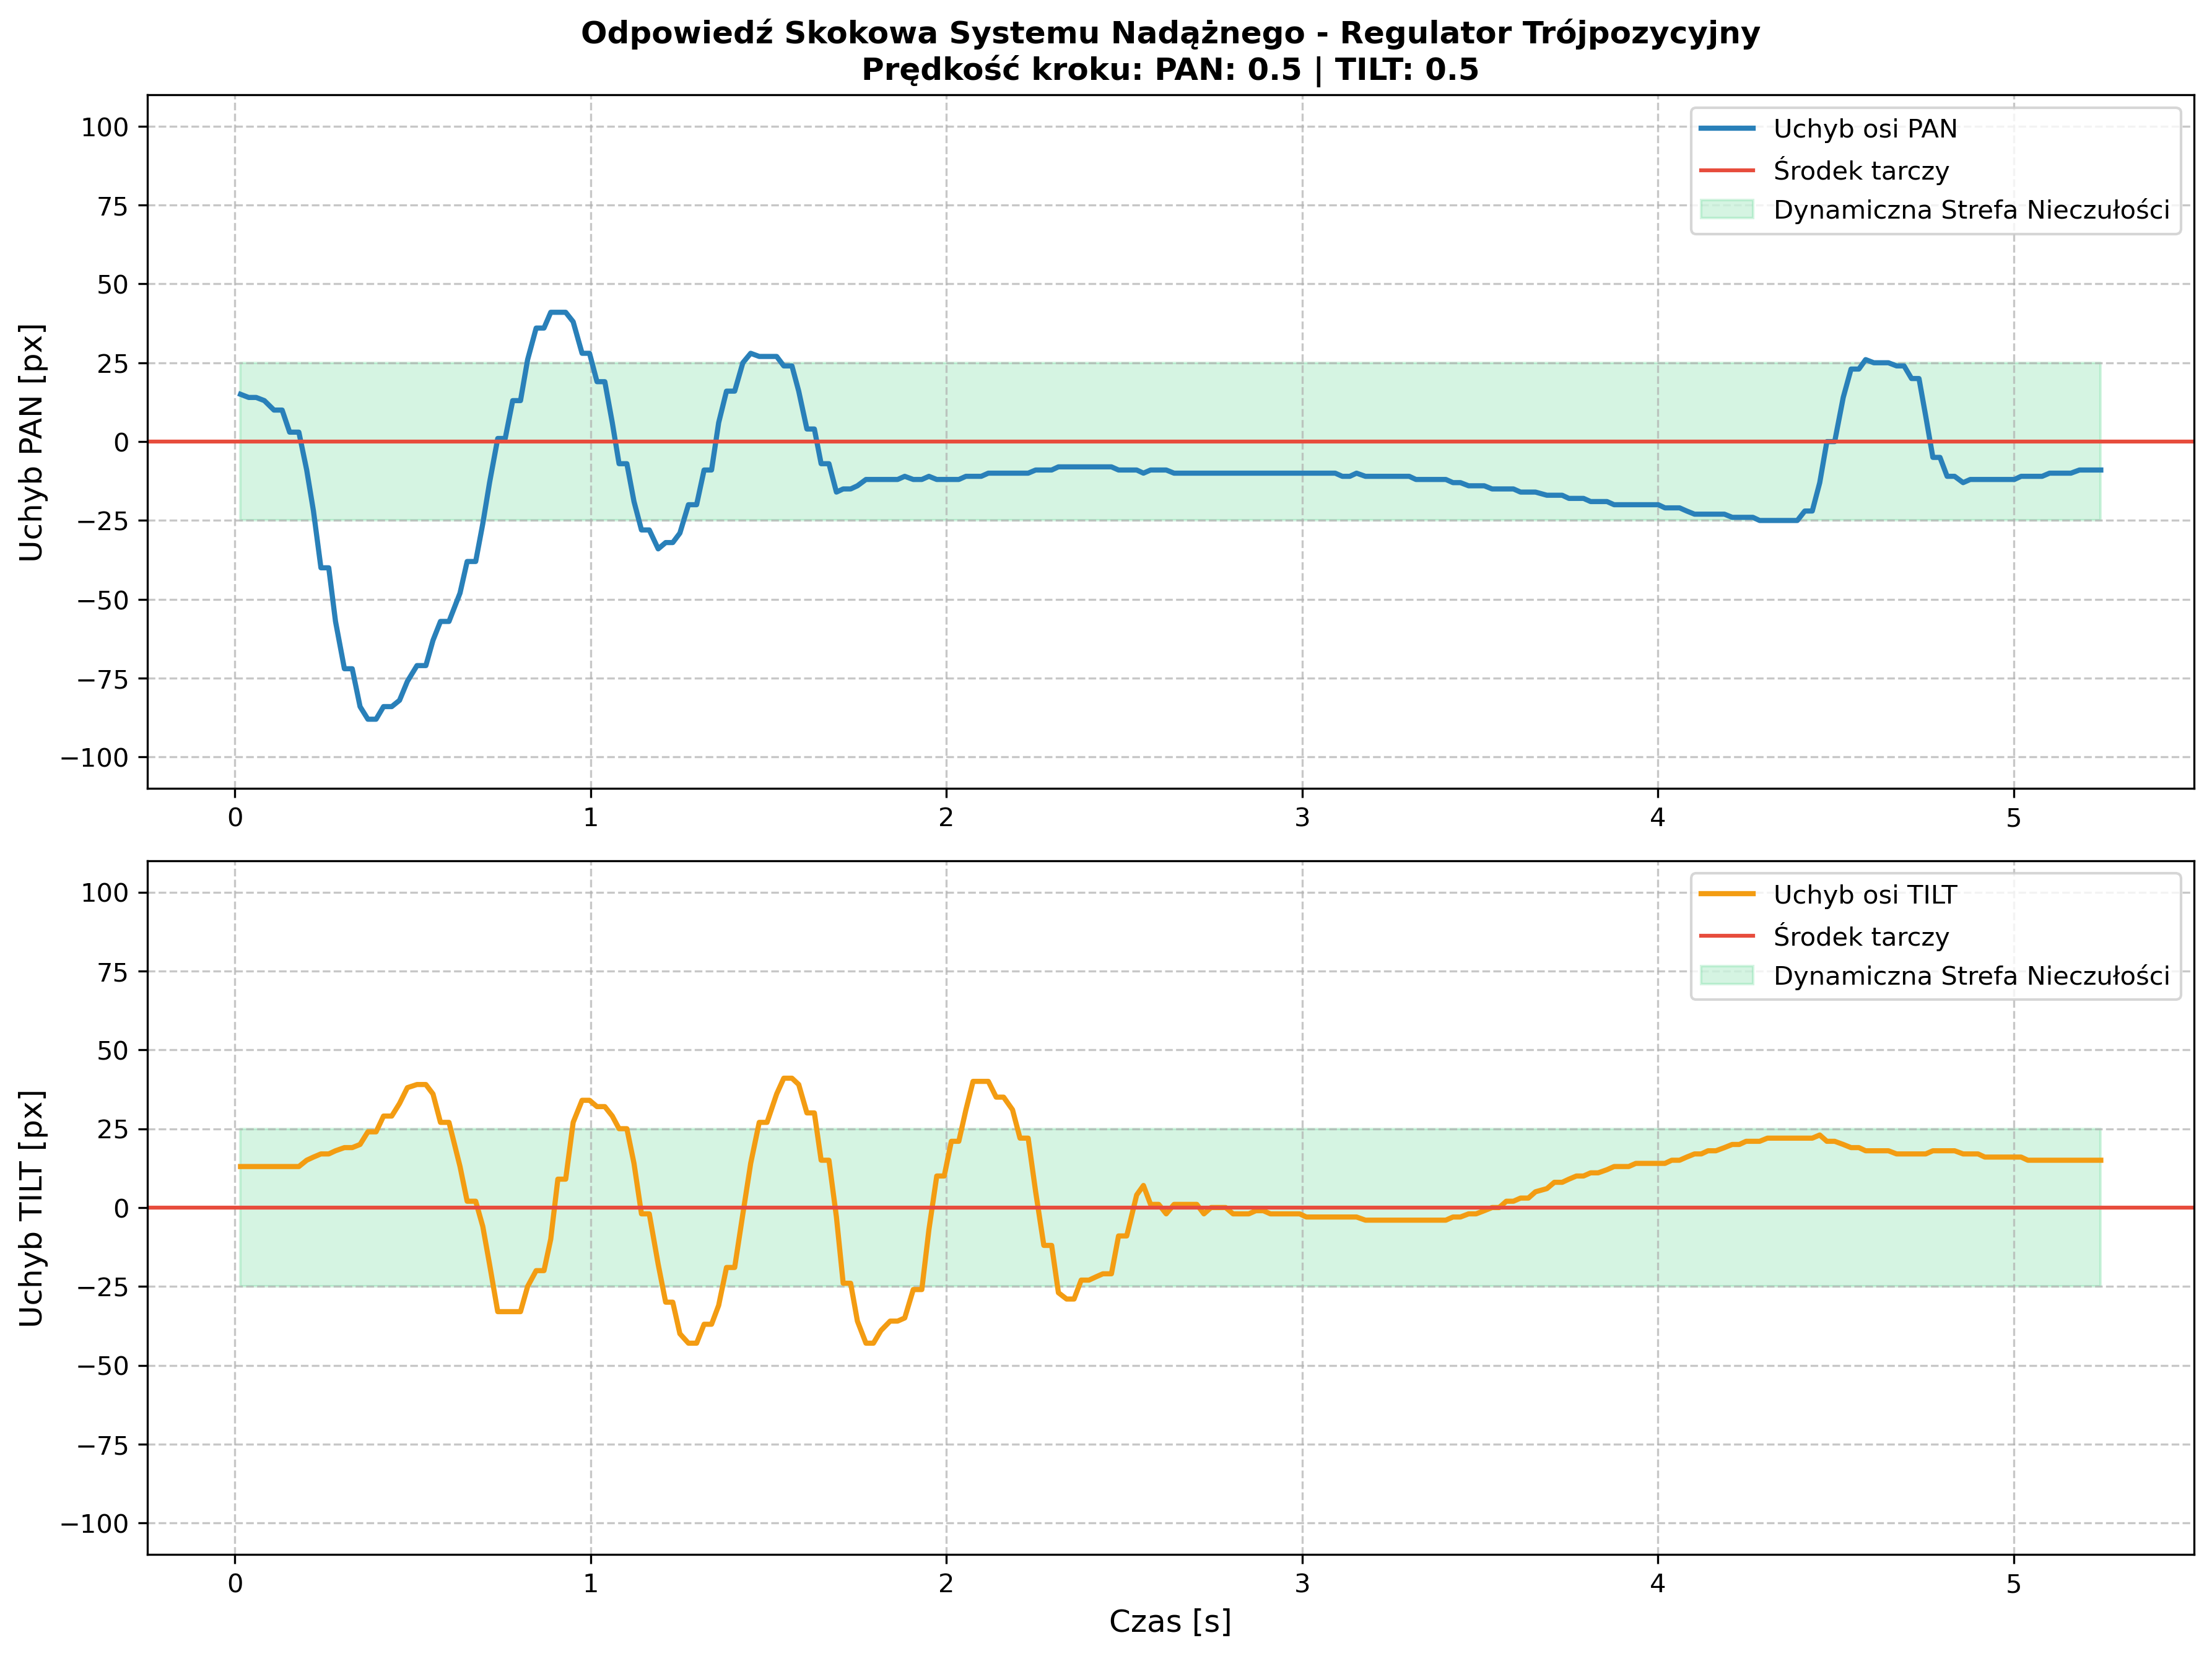
\includegraphics[width=\textwidth]{./Obrazy/WYniki troj/wykres_GOOD_BB_move_150_cm.png}
    \caption{Strefa heurystyczna.}
\end{subfigure}
\hfill
\begin{subfigure}{0.48\textwidth}
    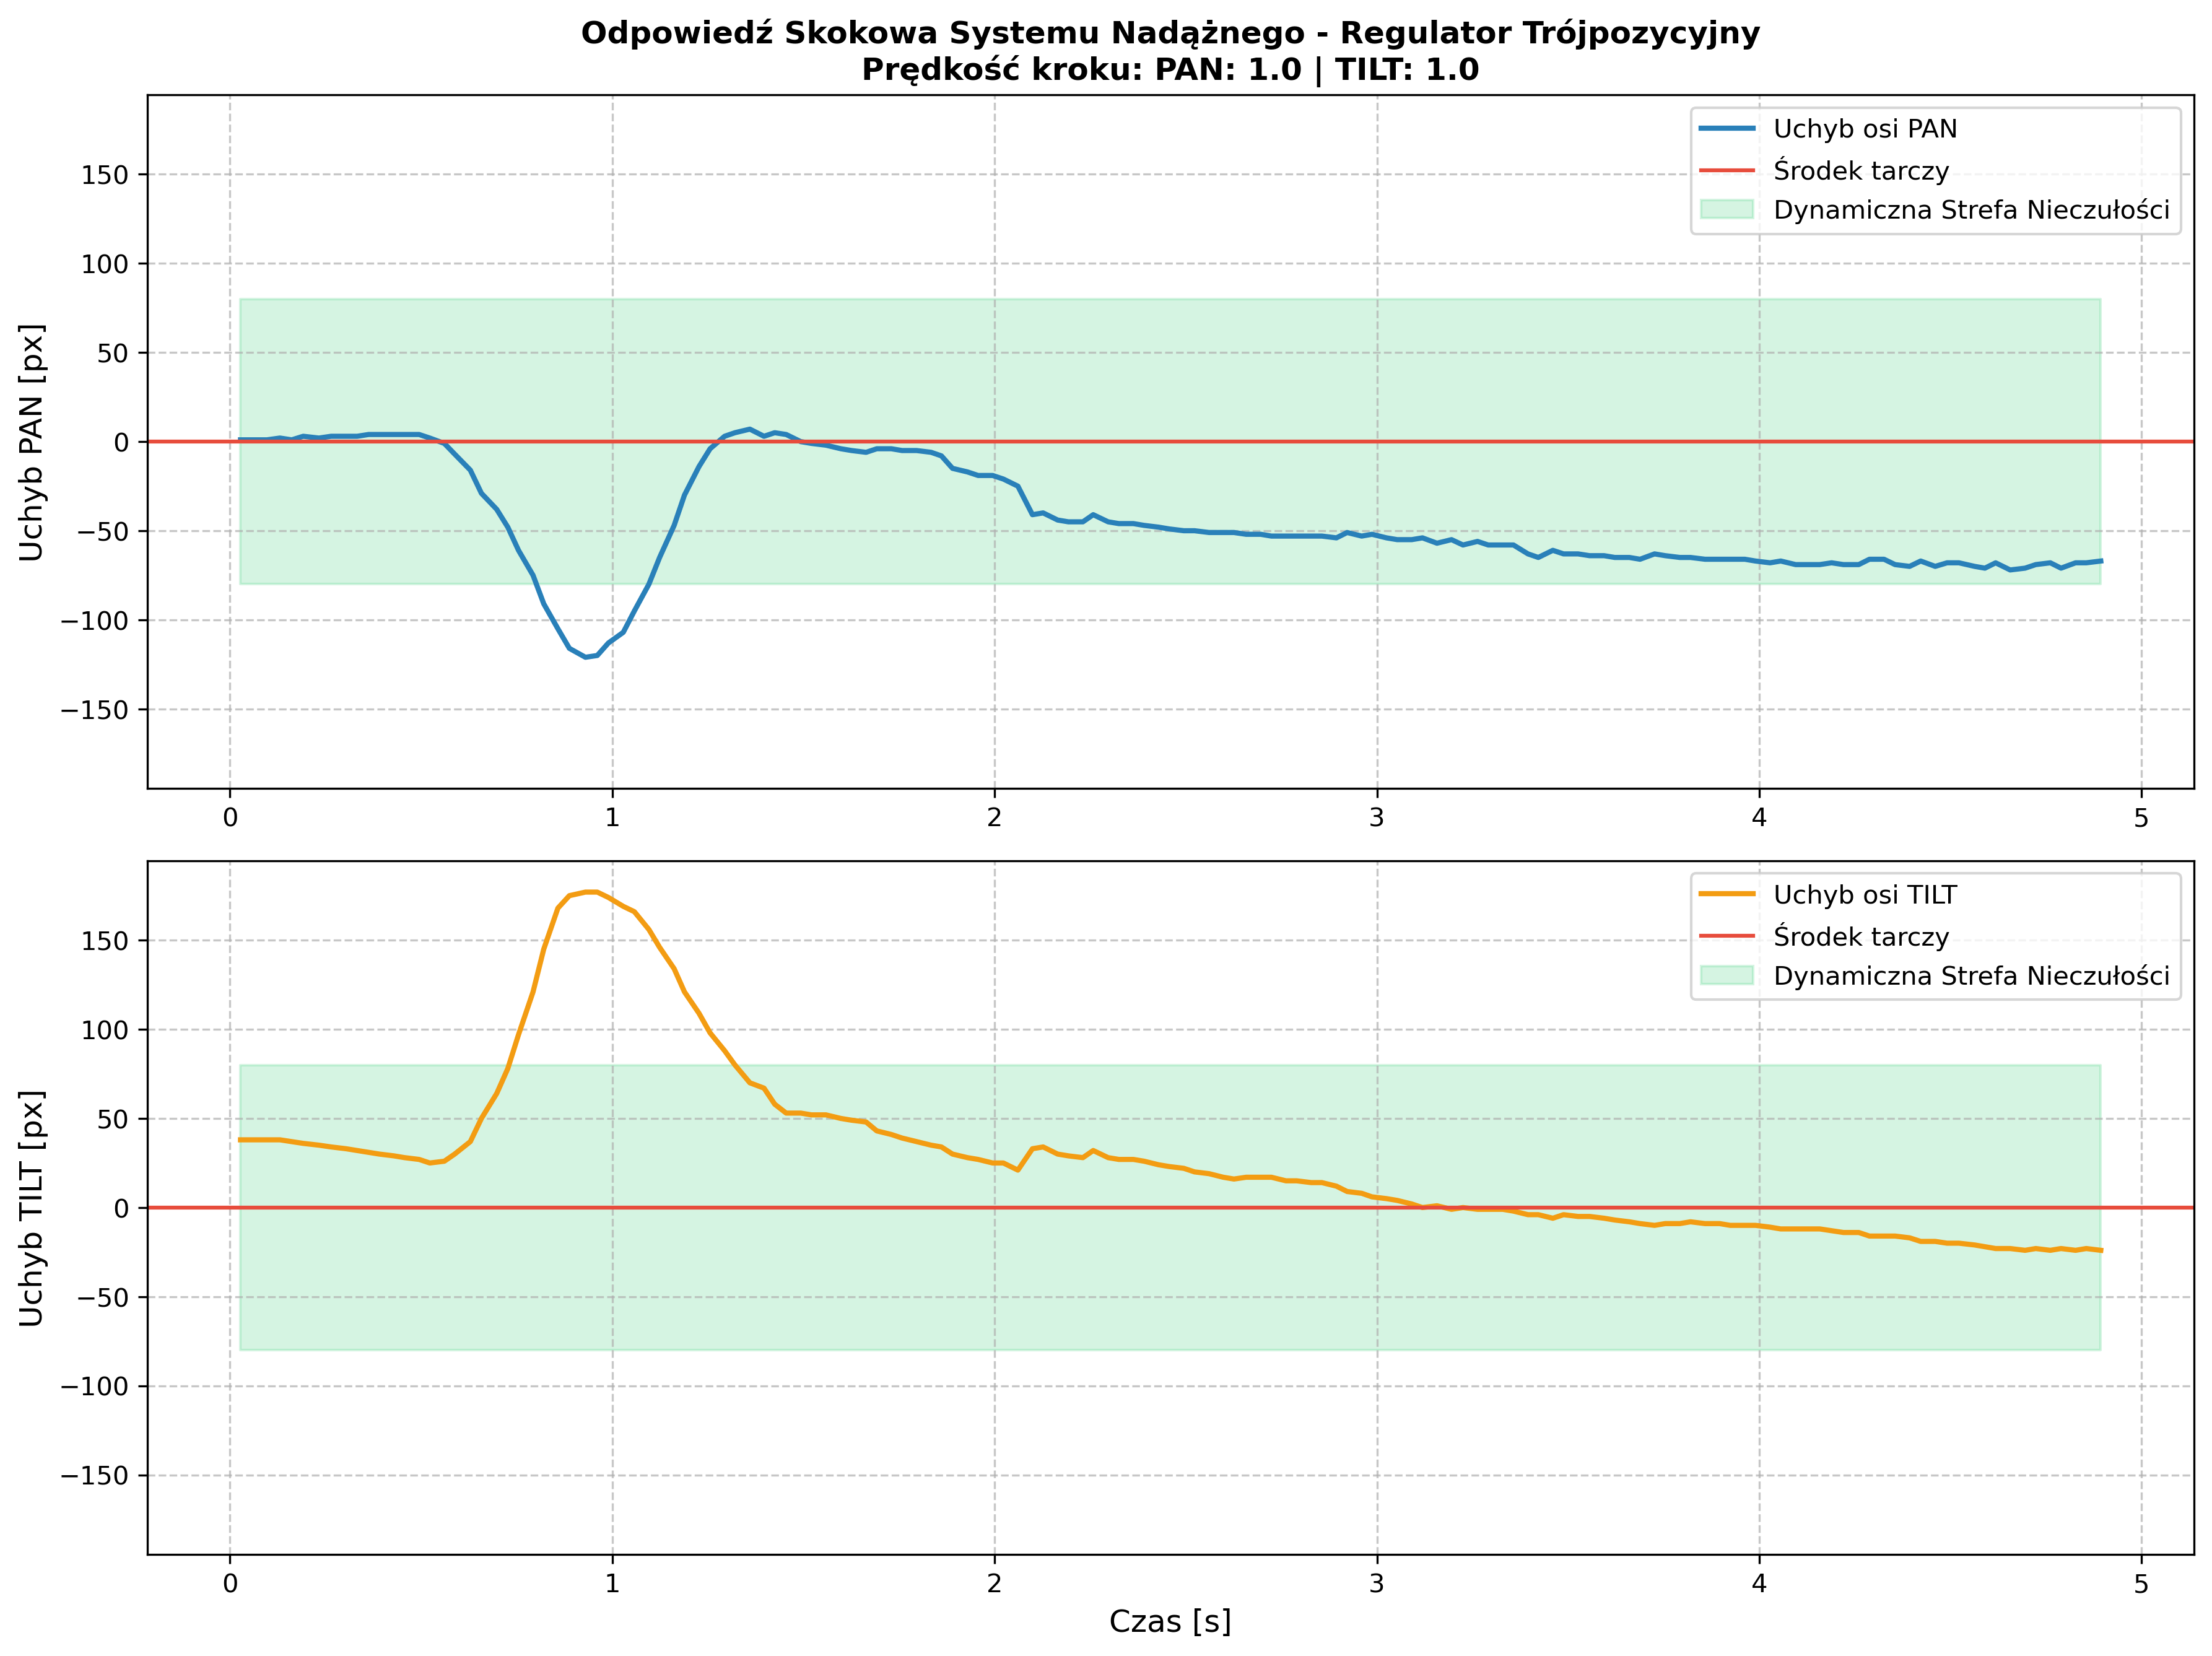
\includegraphics[width=\textwidth]{./Obrazy/WYniki troj/wykres_UP_BB_move_150_cm.png}
    \caption{Strefa analityczna.}
\end{subfigure}
\caption{Porównanie odpowiedzi skokowej regulatora trójpołożeniowego na dystansie 150~cm.}
\label{fig:bb_skok_150}
\end{figure}


\subsection{Śledzenie obiektu poruszającego się po trajektorii okrężnej}
\label{subsec:bb_okrag}

Śledzenie obiektu poruszającego się po trajektorii krzywoliniowej jest niezwykle wymagającym zadaniem dla algorytmu trójpołożeniowego. W przeciwieństwie do regulatorów ciągłych, układ przekaźnikowy nie potrafi płynnie dopasować prędkości obrotowej do płynnego wymuszenia (zmieniającej się prędkości rzutowanej na matrycę). Napędy pracują wyłącznie w trybie pełnej mocy lub całkowitego zatrzymania, co z natury prowadzi do rwanej trajektorii nadążania.

Podczas jednoczesnej pracy osi PAN i TILT na optymalnym dystansie $80$~cm (rys. \ref{fig:bb_okrag_80}), wąska strefa heurystyczna powodowała bardzo wysoką częstotliwość przełączeń. Ze względu na ciągły ruch celu, uchyb błyskawicznie opuszczał strefę tolerancji, wymuszając nieustanne, nerwowe korekty. Zjawisko to (tzw. \textit{chattering}) jest skrajnie niekorzystne z punktu widzenia trwałości przekładni mechanicznych. Zastosowanie szerokiej, wyliczonej analitycznie strefy nieczułości drastycznie obniżyło częstotliwość przełączeń silników. Cel zyskał margines na swobodne przemieszczanie się wewnątrz powiększonego obszaru tolerancji, co na wykresie \ref{fig:bb_okrag_80}b objawia się charakterystycznymi wypłaszczeniami wewnątrz zielonej strefy. Choć chwilowy błąd bezwzględny jest większy, kultura pracy napędów uległa radykalnej poprawie.

\begin{figure}[!ht]
\centering
\begin{subfigure}{0.48\textwidth}
    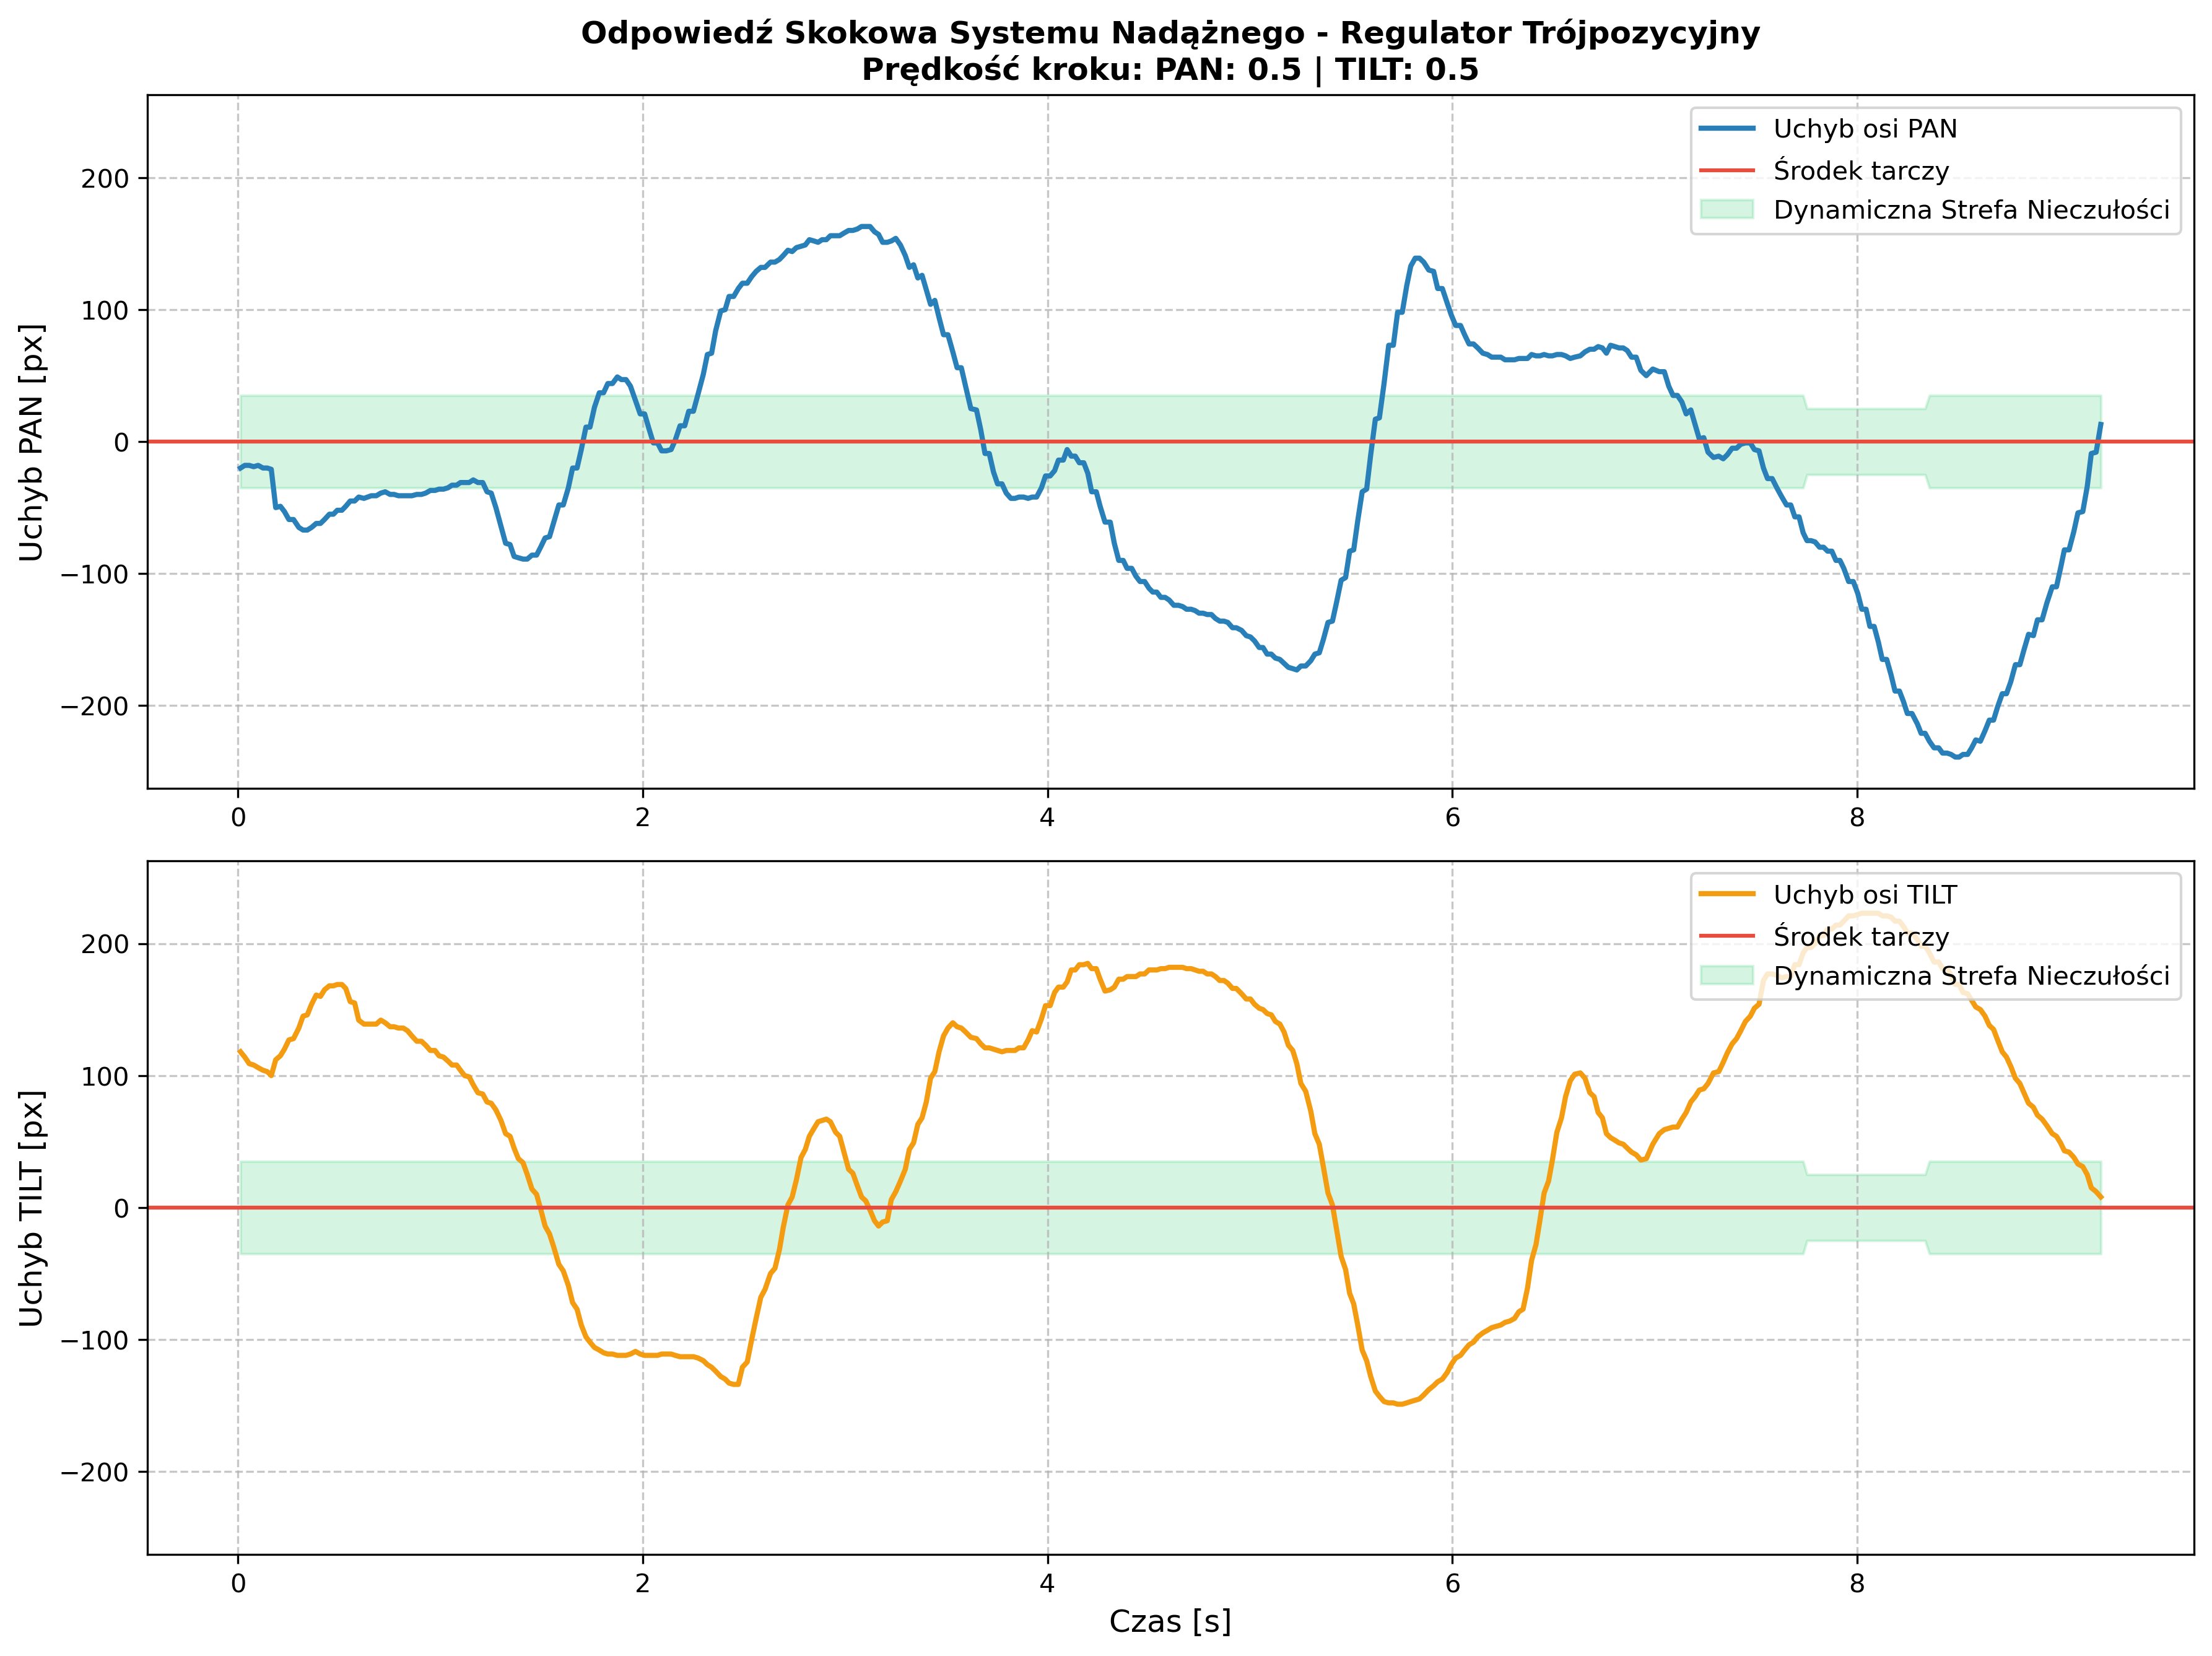
\includegraphics[width=\textwidth]{./Obrazy/WYniki troj/wykres_GOOD_BB_circural_80_cm.png}
    \caption{Strefa heurystyczna.}
\end{subfigure}
\hfill
\begin{subfigure}{0.48\textwidth}
    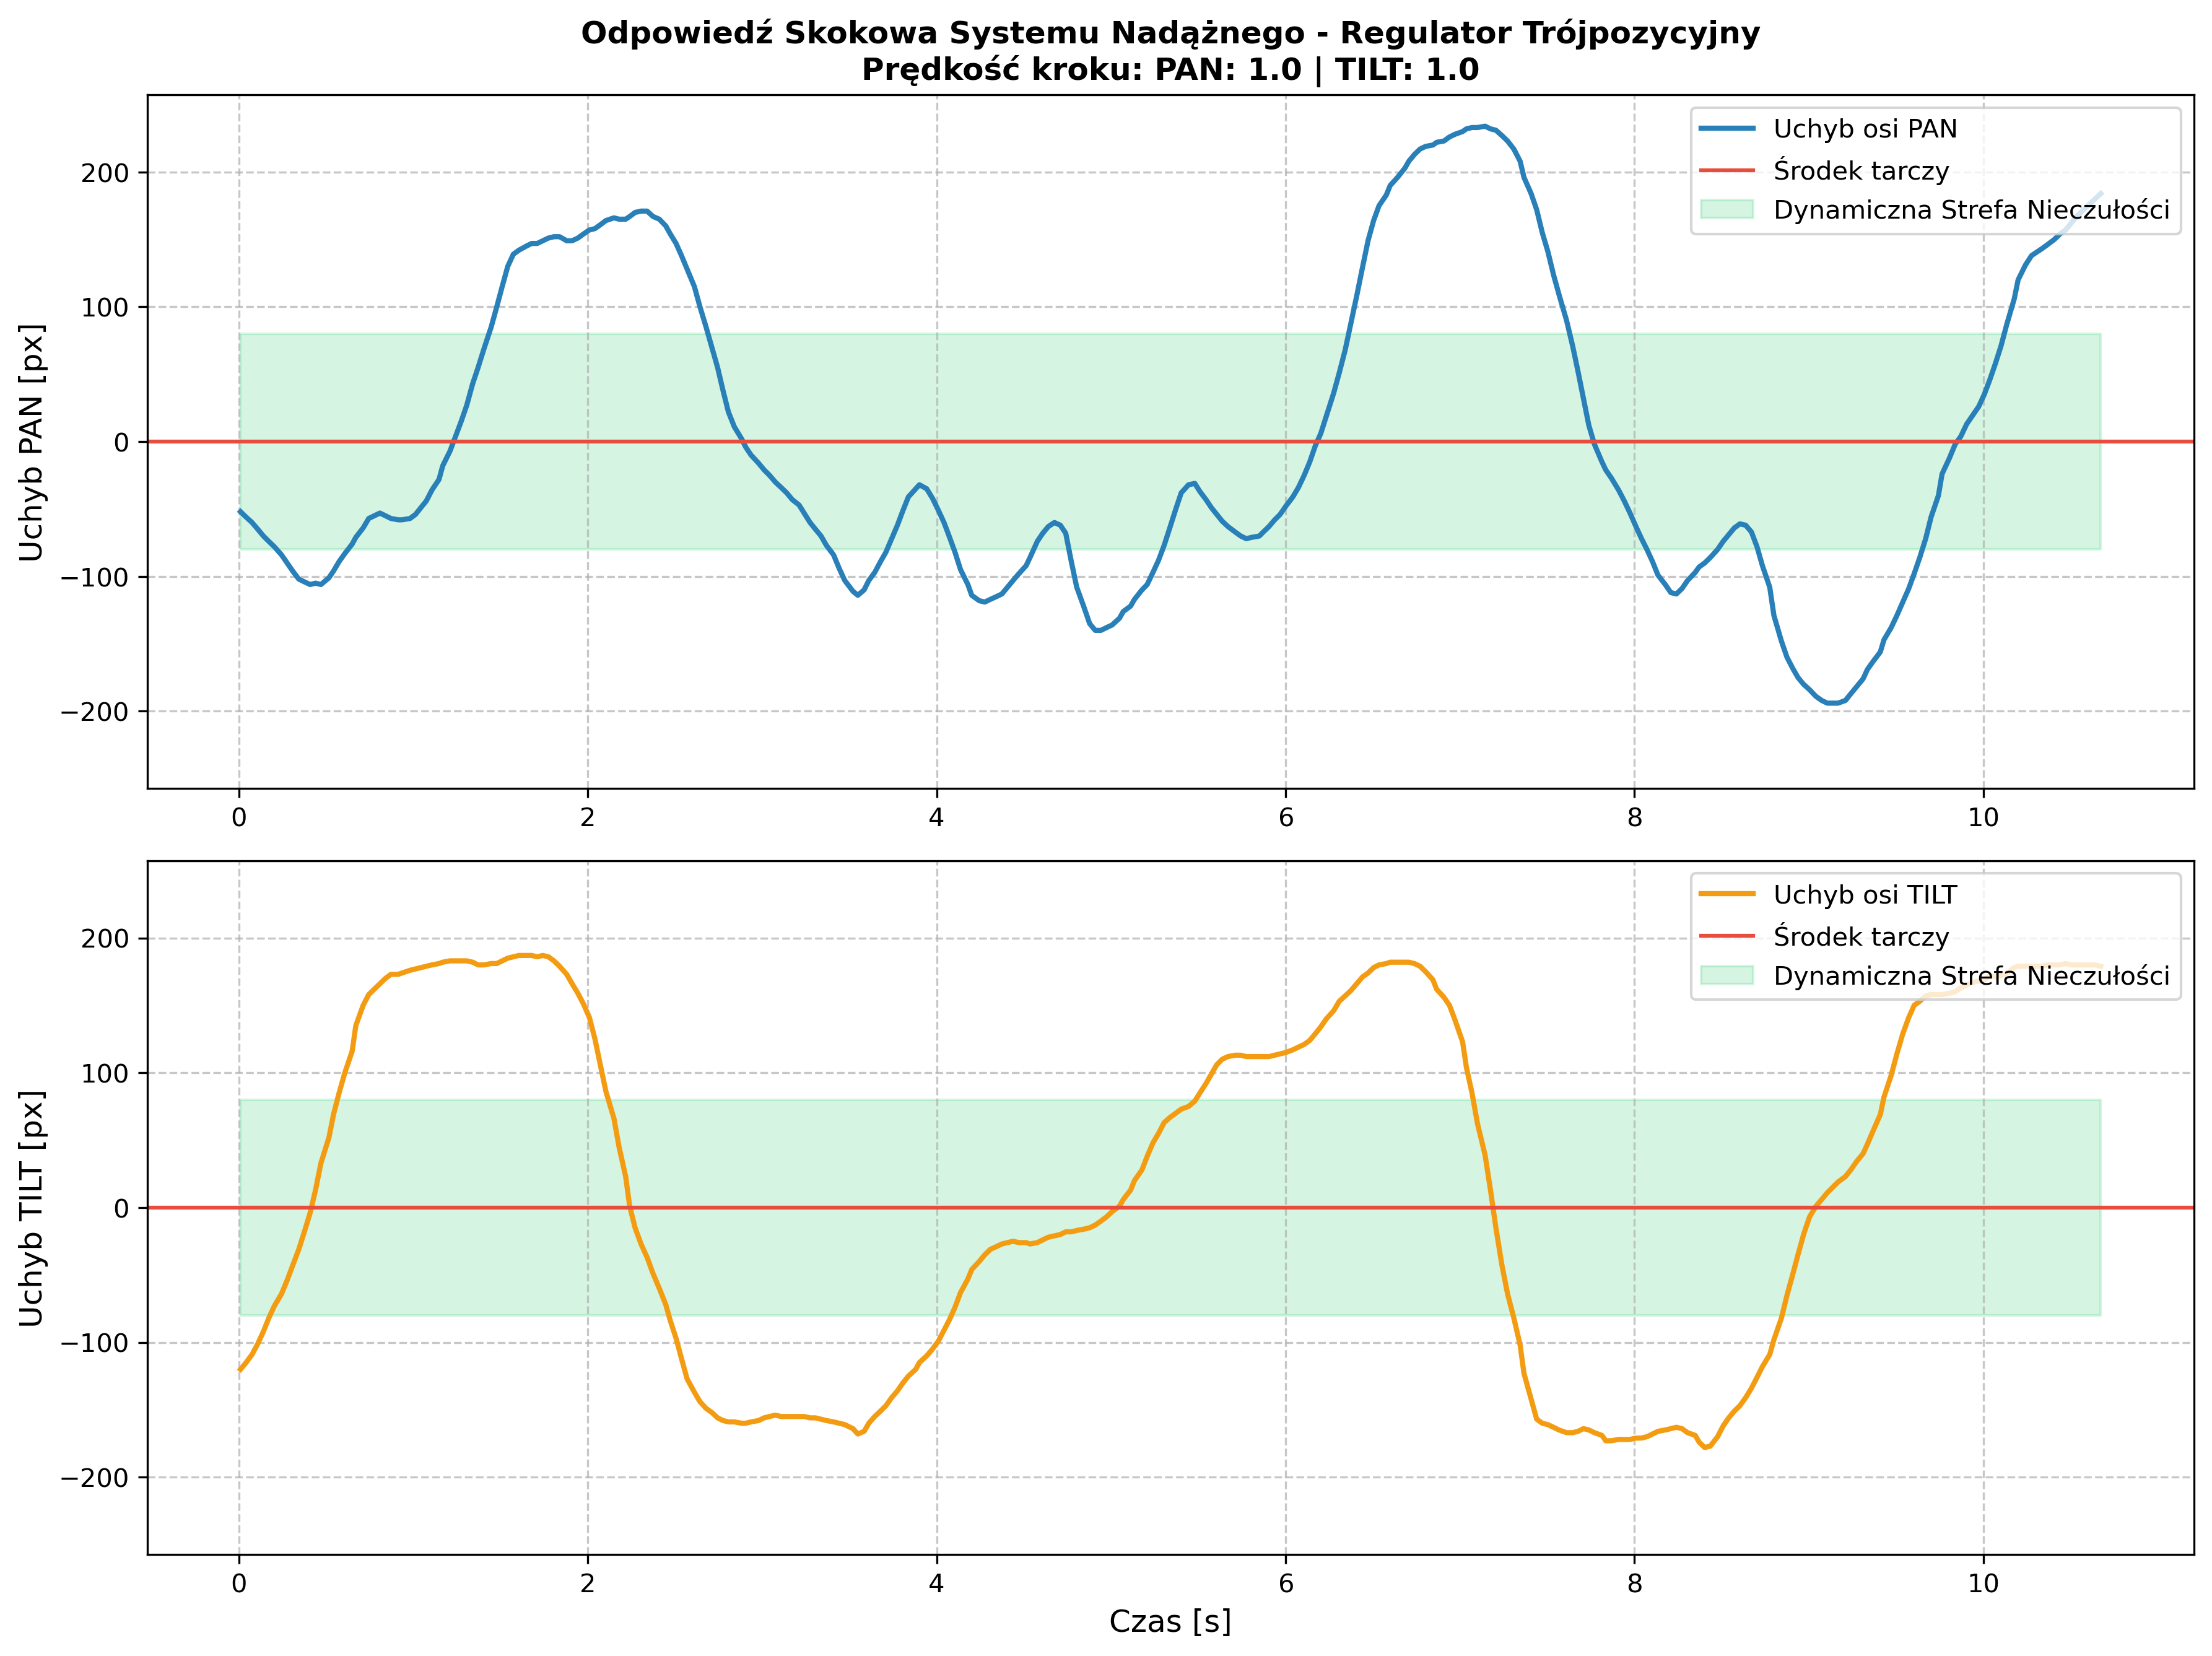
\includegraphics[width=\textwidth]{./Obrazy/WYniki troj/wykres_UP_BB_circural_80_cm.png}
    \caption{Strefa analityczna.}
\end{subfigure}
\caption{Śledzenie ruchu okrężnego dla dystansu 80~cm (Regulator trójpołożeniowy).}
\label{fig:bb_okrag_80}
\end{figure}

Zmniejszenie odległości do $30$~cm (rys. \ref{fig:bb_okrag_30}) obnażyło kinematyczne ograniczenia wieżyczki sterowanej przekaźnikowo. Ze względu na olbrzymią pozorną prędkość kątową celu, uchyb w wariancie heurystycznym przyjął postać regularnej fali o amplitudzie przekraczającej $200$ pikseli. Układ nie nadążał za obiektem, przeskakując z opóźnieniem między skrajnymi wychyleniami. Zastosowanie nastaw analitycznych z odpowiednio poszerzoną strefą zniwelowało zjawisko wysokoczęstotliwościowych uderzeń. Napędy załączały się rzadziej, asymilując energię błędów w szerokim buforze, co pozwoliło utrzymać obiekt w kadrze pomimo widocznego opóźnienia fazowego.

\begin{figure}[!ht]
\centering
\begin{subfigure}{0.48\textwidth}
    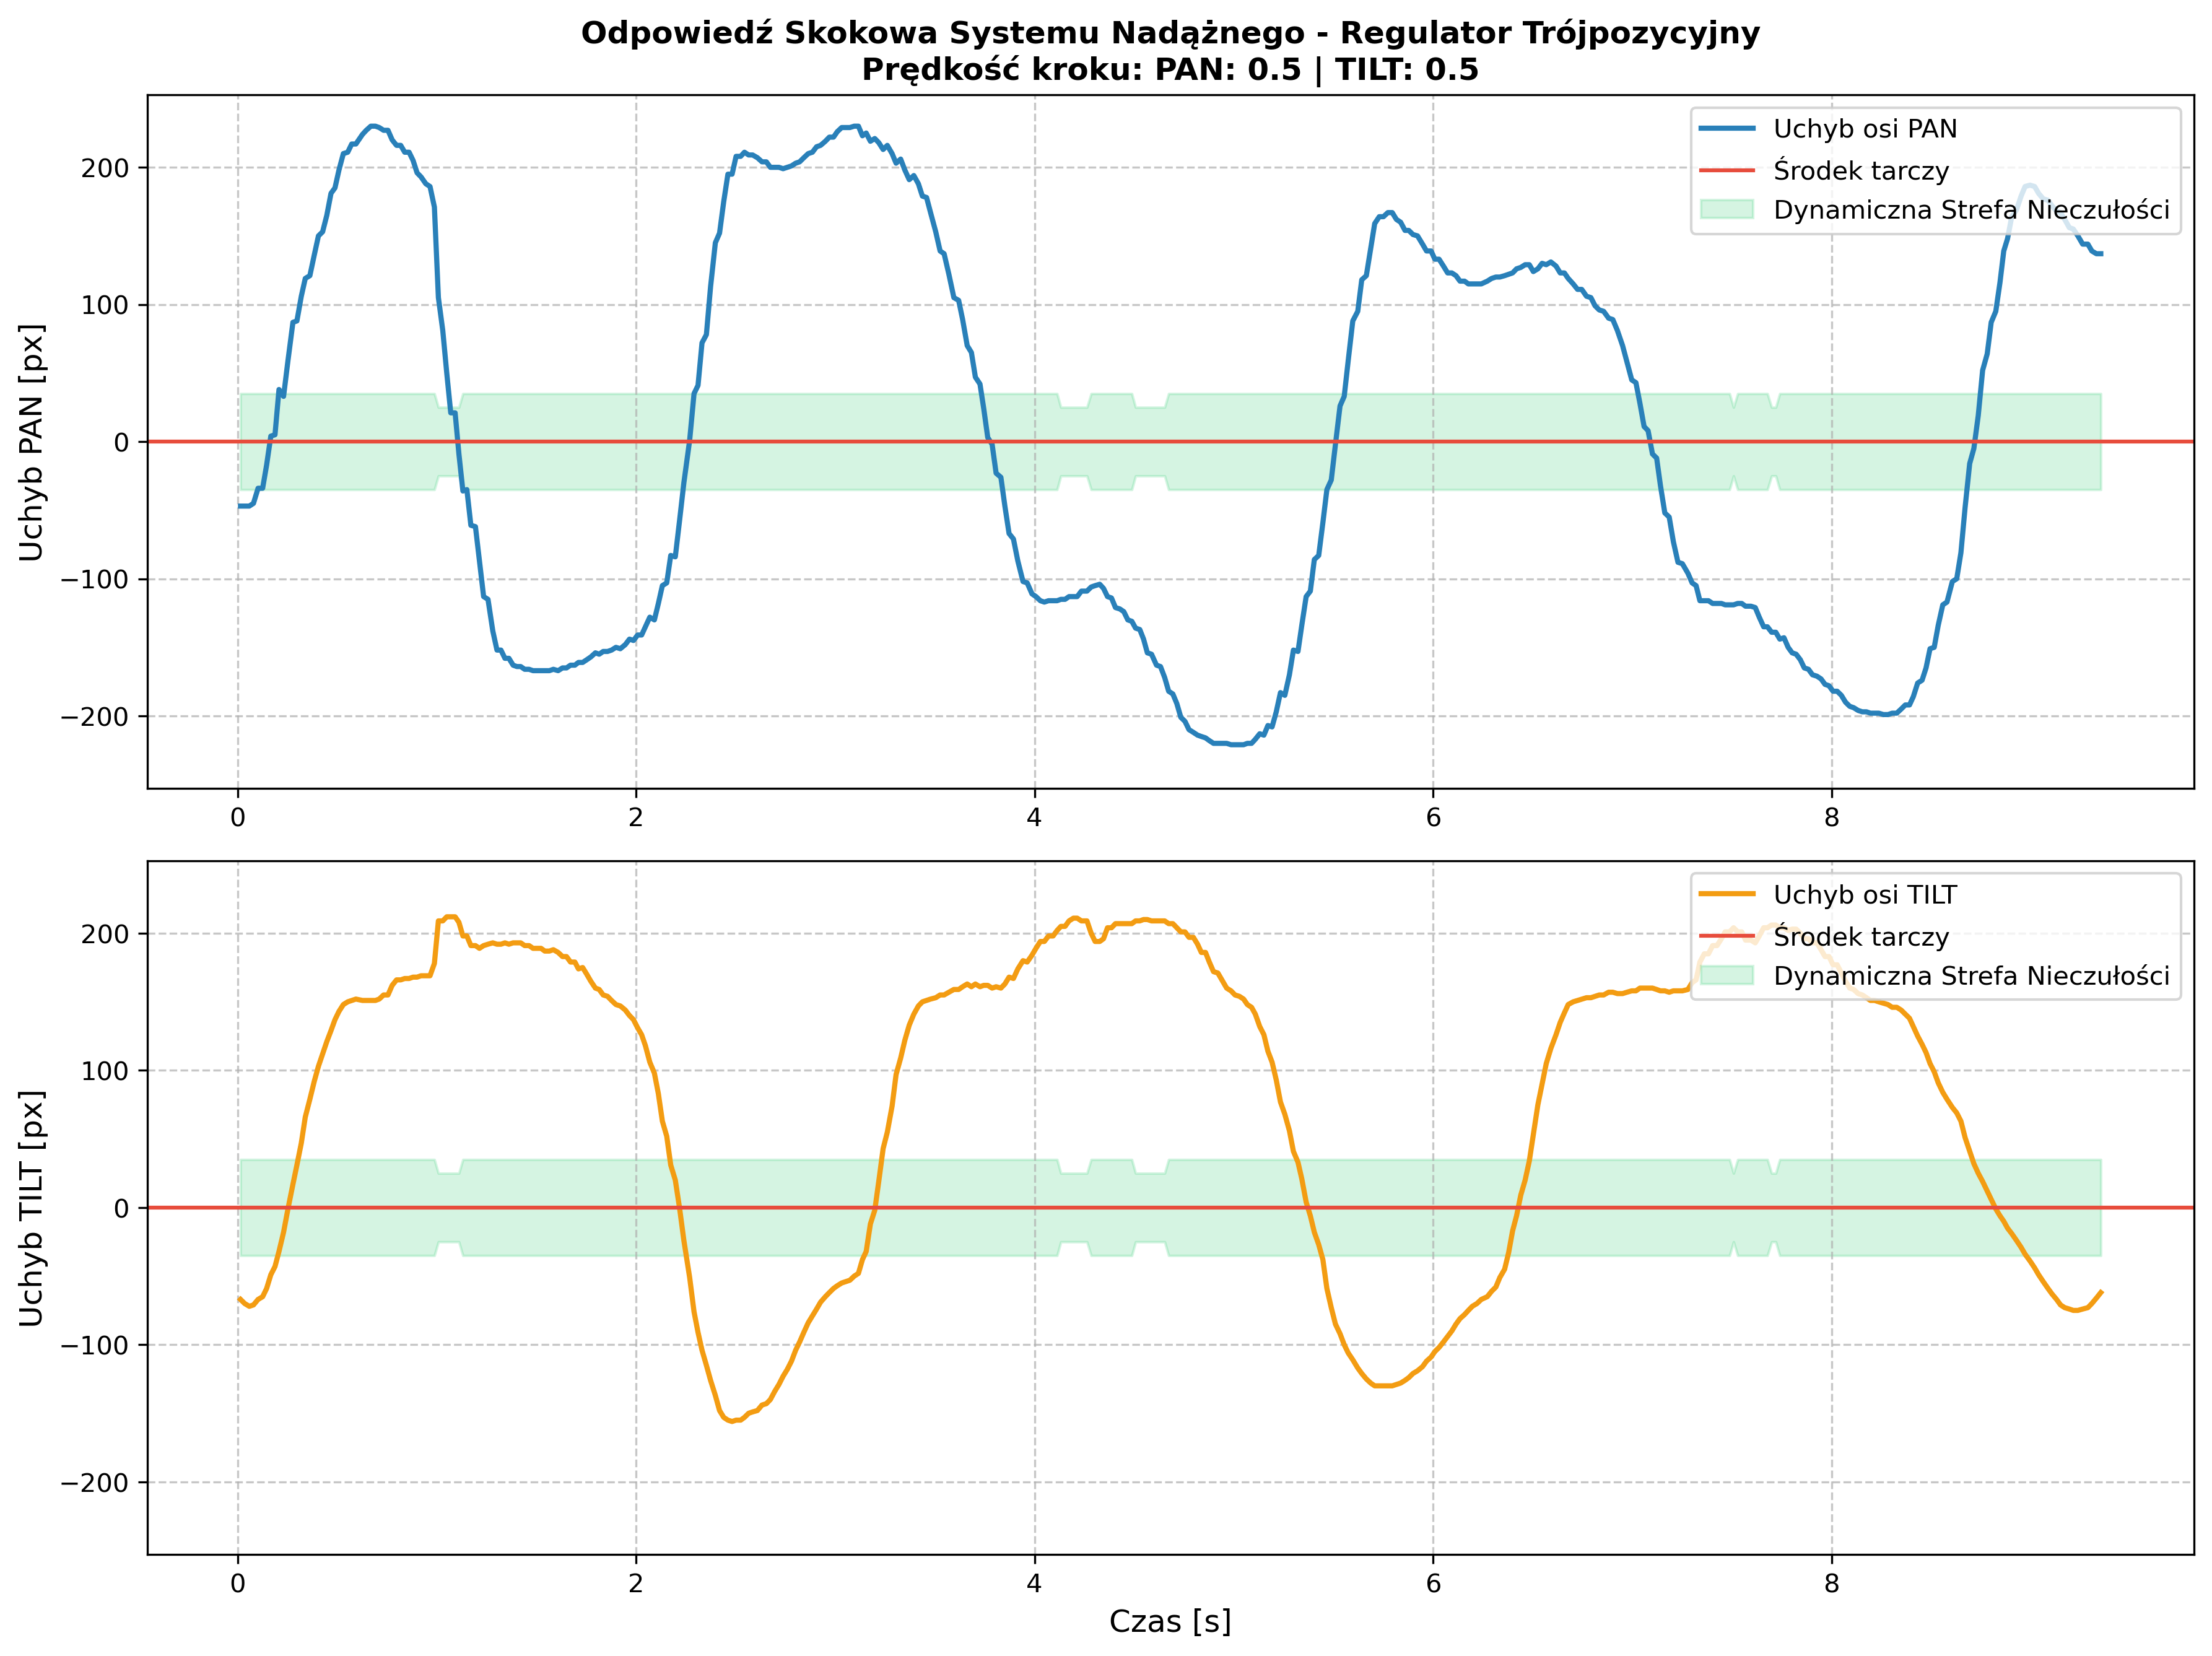
\includegraphics[width=\textwidth]{./Obrazy/WYniki troj/wykres_GOOD_BB_circural_30_cm.png}
    \caption{Strefa heurystyczna.}
\end{subfigure}
\hfill
\begin{subfigure}{0.48\textwidth}
    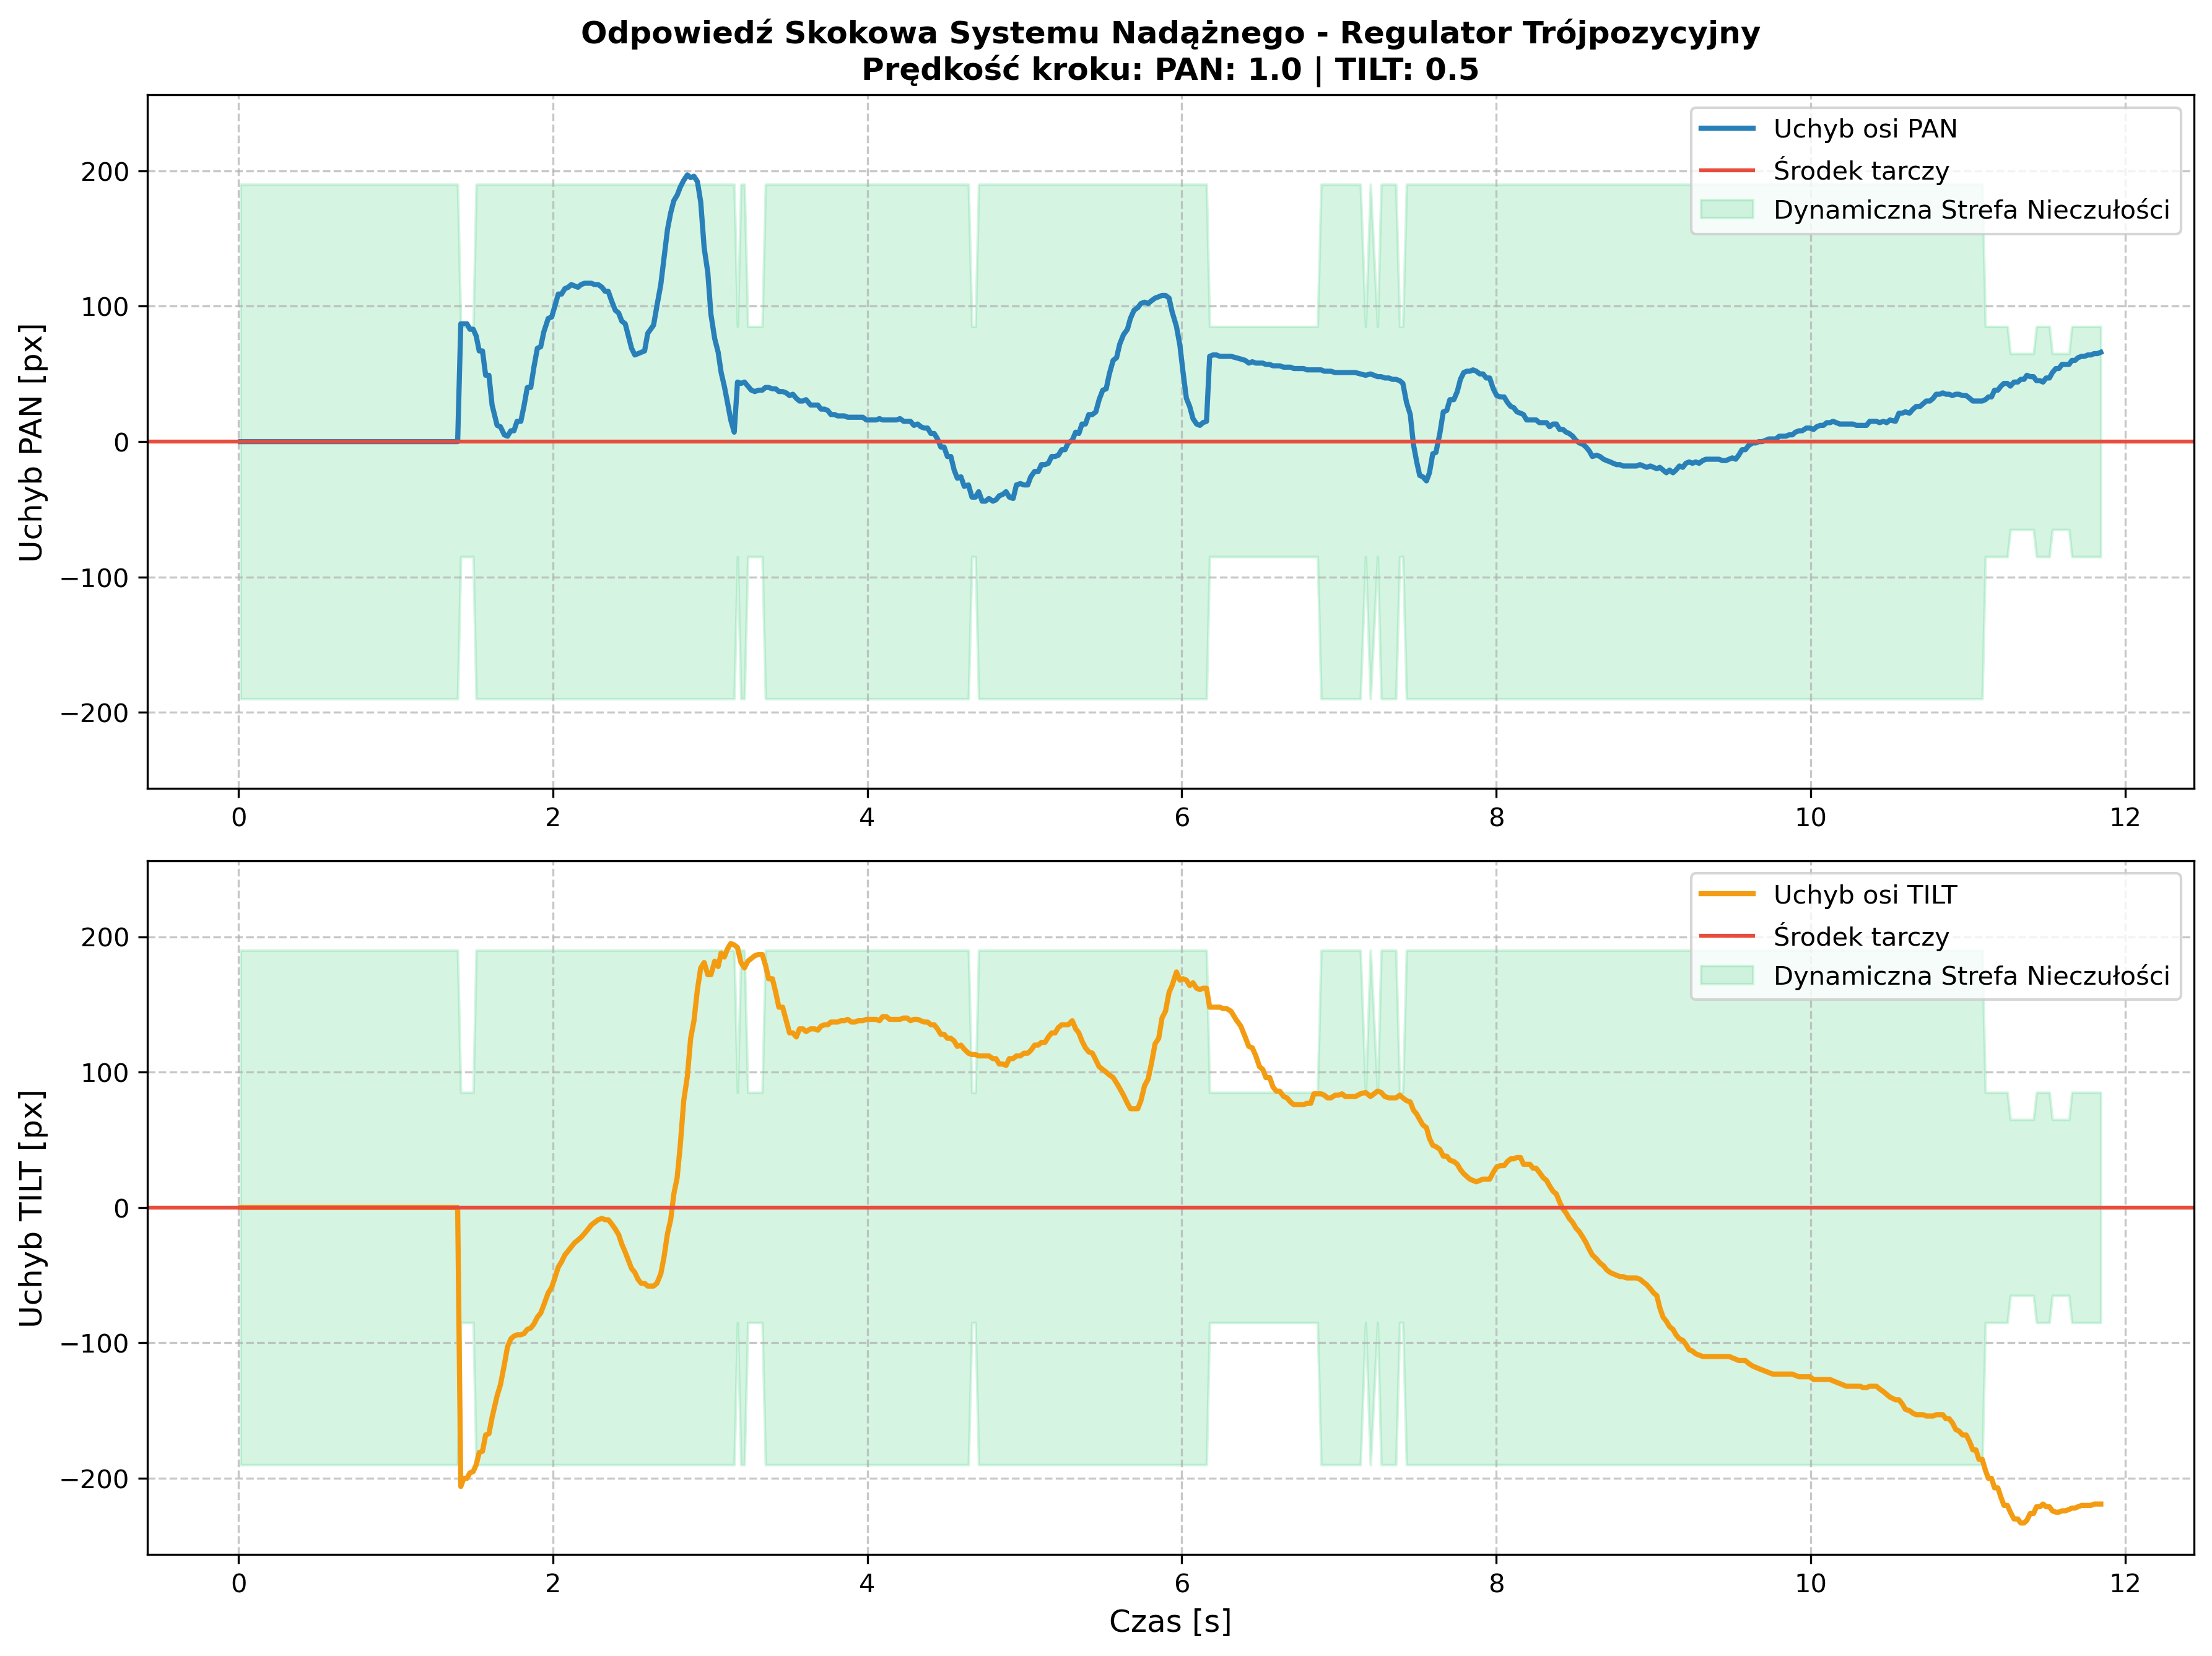
\includegraphics[width=\textwidth]{./Obrazy/WYniki troj/wykres_UP_BB_circural_30_cm.png}
    \caption{Strefa analityczna.}
\end{subfigure}
\caption{Śledzenie ruchu okrężnego dla dystansu 30~cm (Regulator trójpołożeniowy).}
\label{fig:bb_okrag_30}
\end{figure}

Testy na dystansie $150$~cm (rys. \ref{fig:bb_okrag_150}) udowodniły skuteczność adaptacyjnej zmiany strefy nieczułości. W wariancie heurystycznym (stała, wąska strefa w całym zakresie) widoczne są ciągłe, nerwowe oscylacje o małej amplitudzie, powstające podczas prób wycentrowania oddalonego obiektu. Wdrożenie algorytmu modyfikującego korytarz tolerancji na podstawie wielkości obiektu na matrycy uspokoiło odpowiedź układu (rys. \ref{fig:bb_okrag_150}b). Błąd jest bezpiecznie zamykany wewnątrz zwężonej, dynamicznej strefy, eliminując niepotrzebne mikro-ruchy serwomechanizmów i stabilizując trajektorię obserwacji.

\begin{figure}[!ht]
\centering
\begin{subfigure}{0.48\textwidth}
    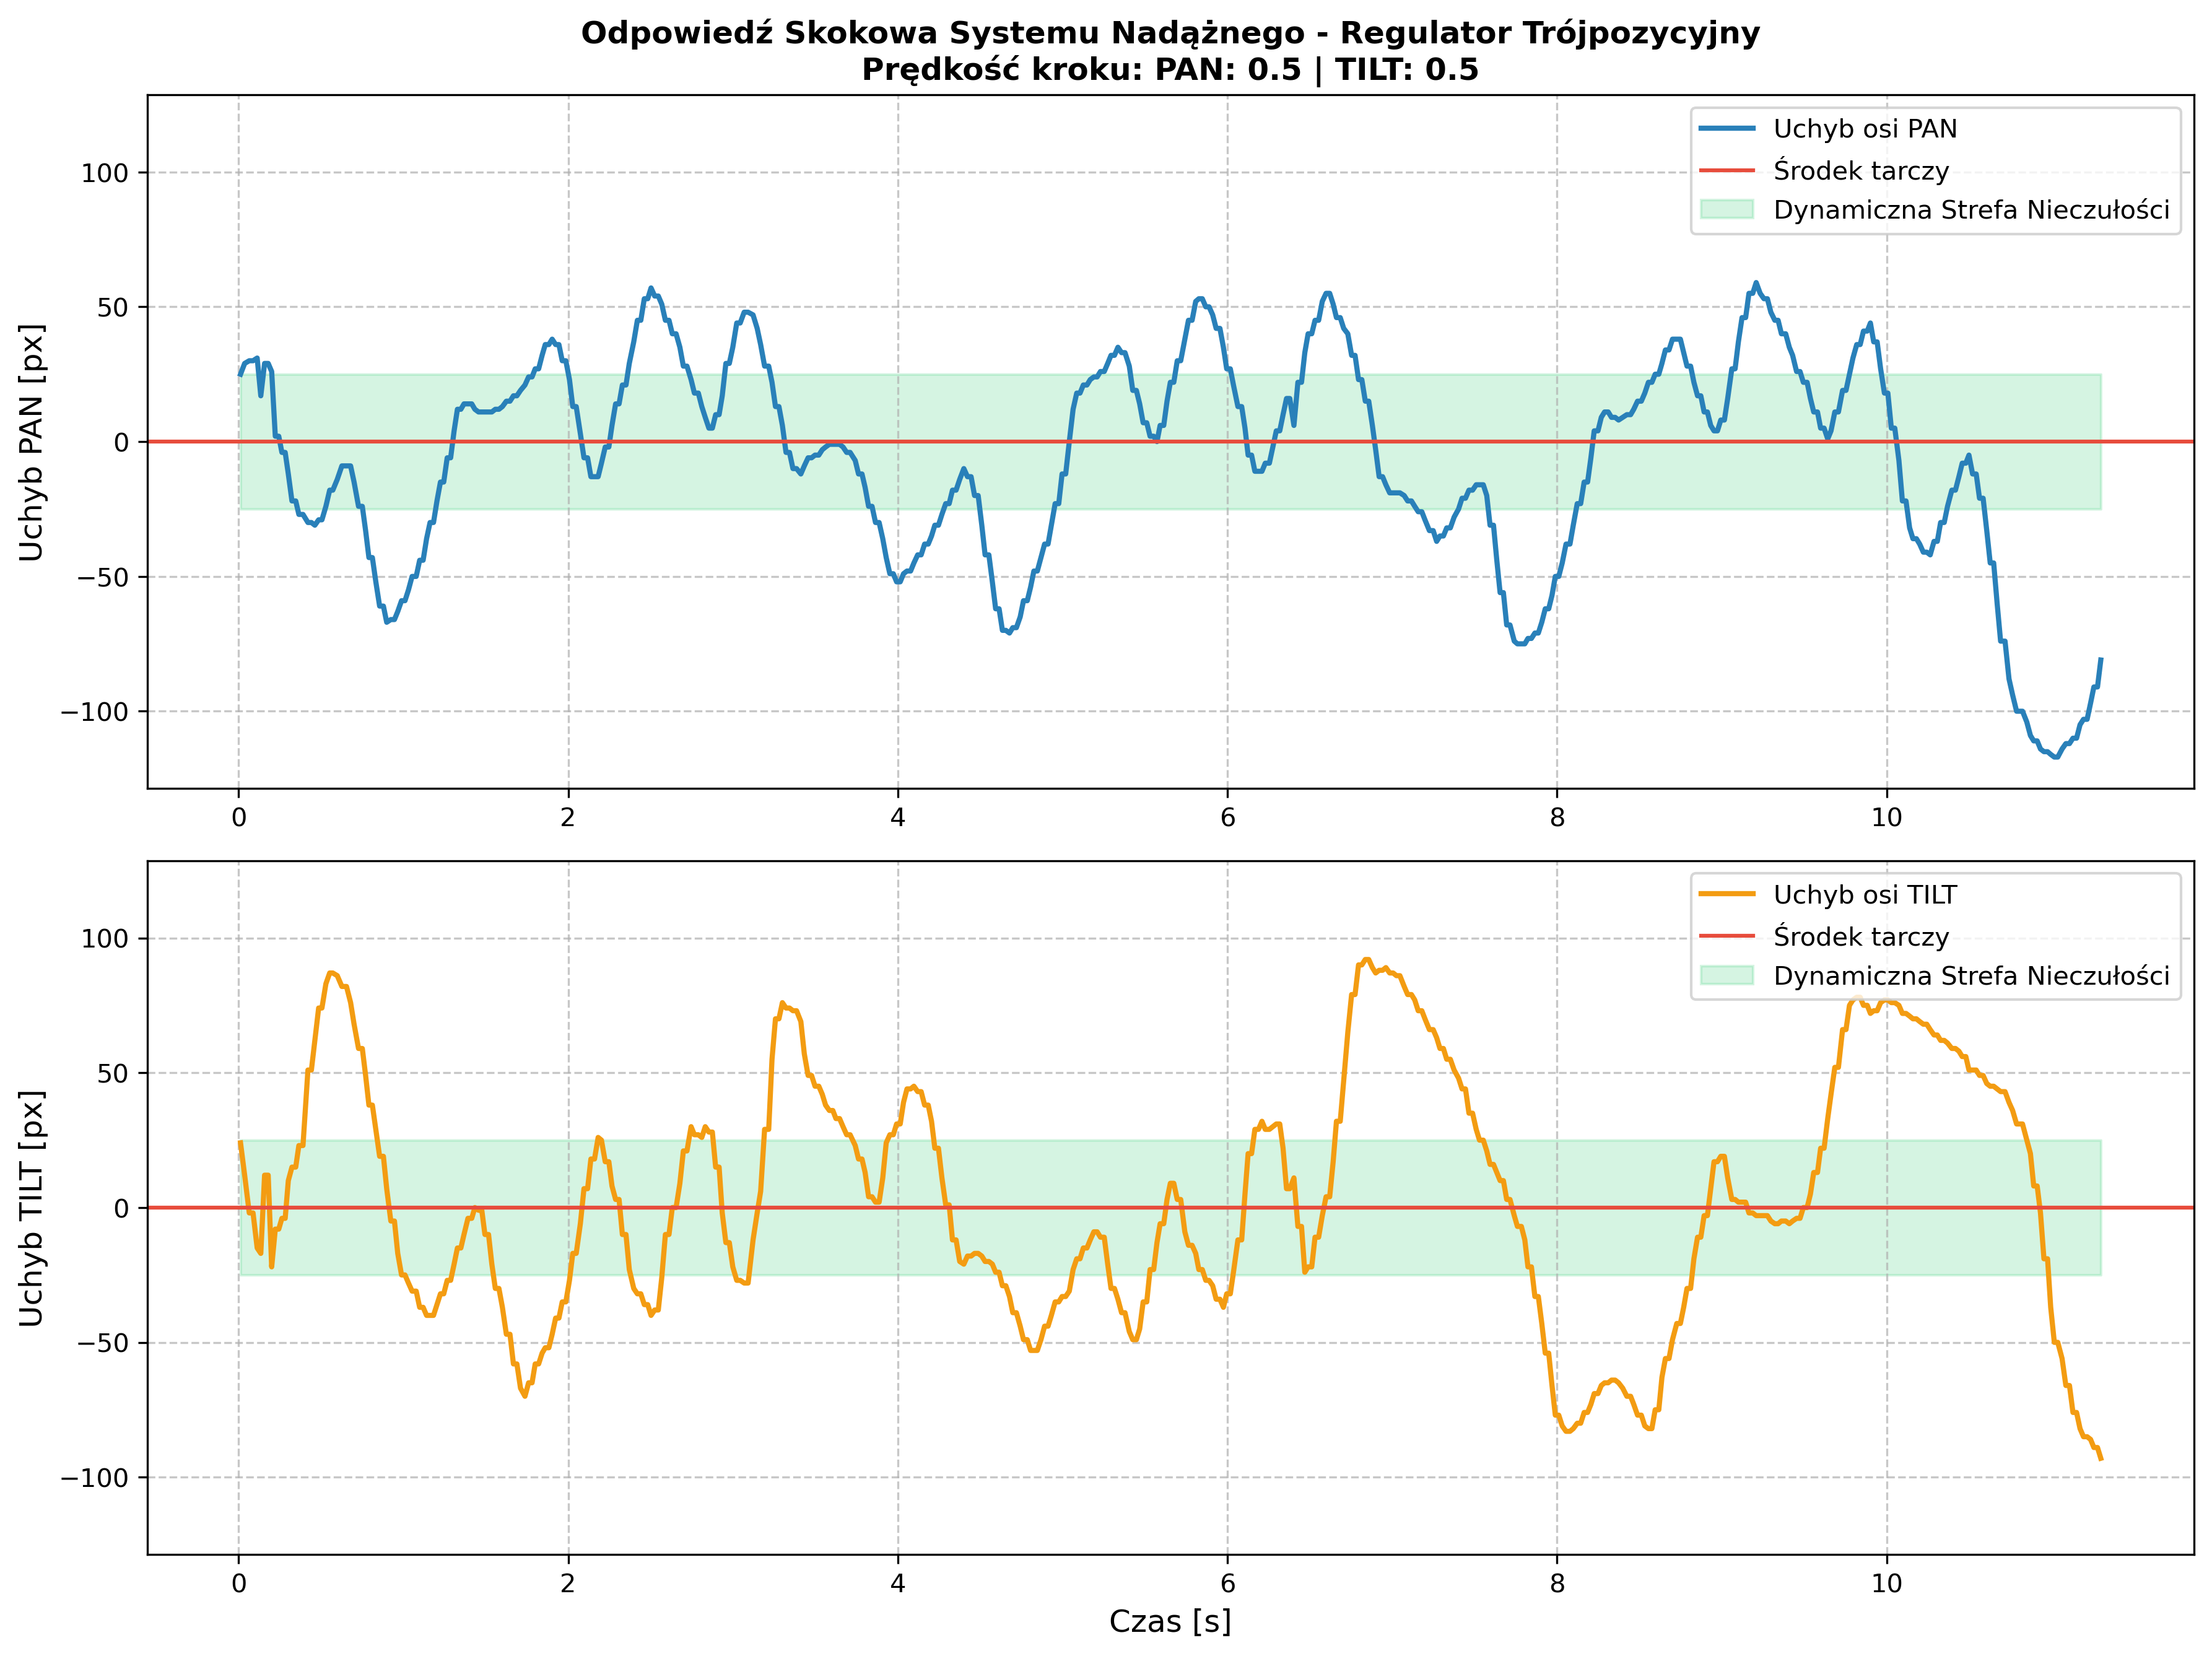
\includegraphics[width=\textwidth]{./Obrazy/WYniki troj/wykres_GOOD_BB_circural_150_cm.png}
    \caption{Strefa heurystyczna.}
\end{subfigure}
\hfill
\begin{subfigure}{0.48\textwidth}
    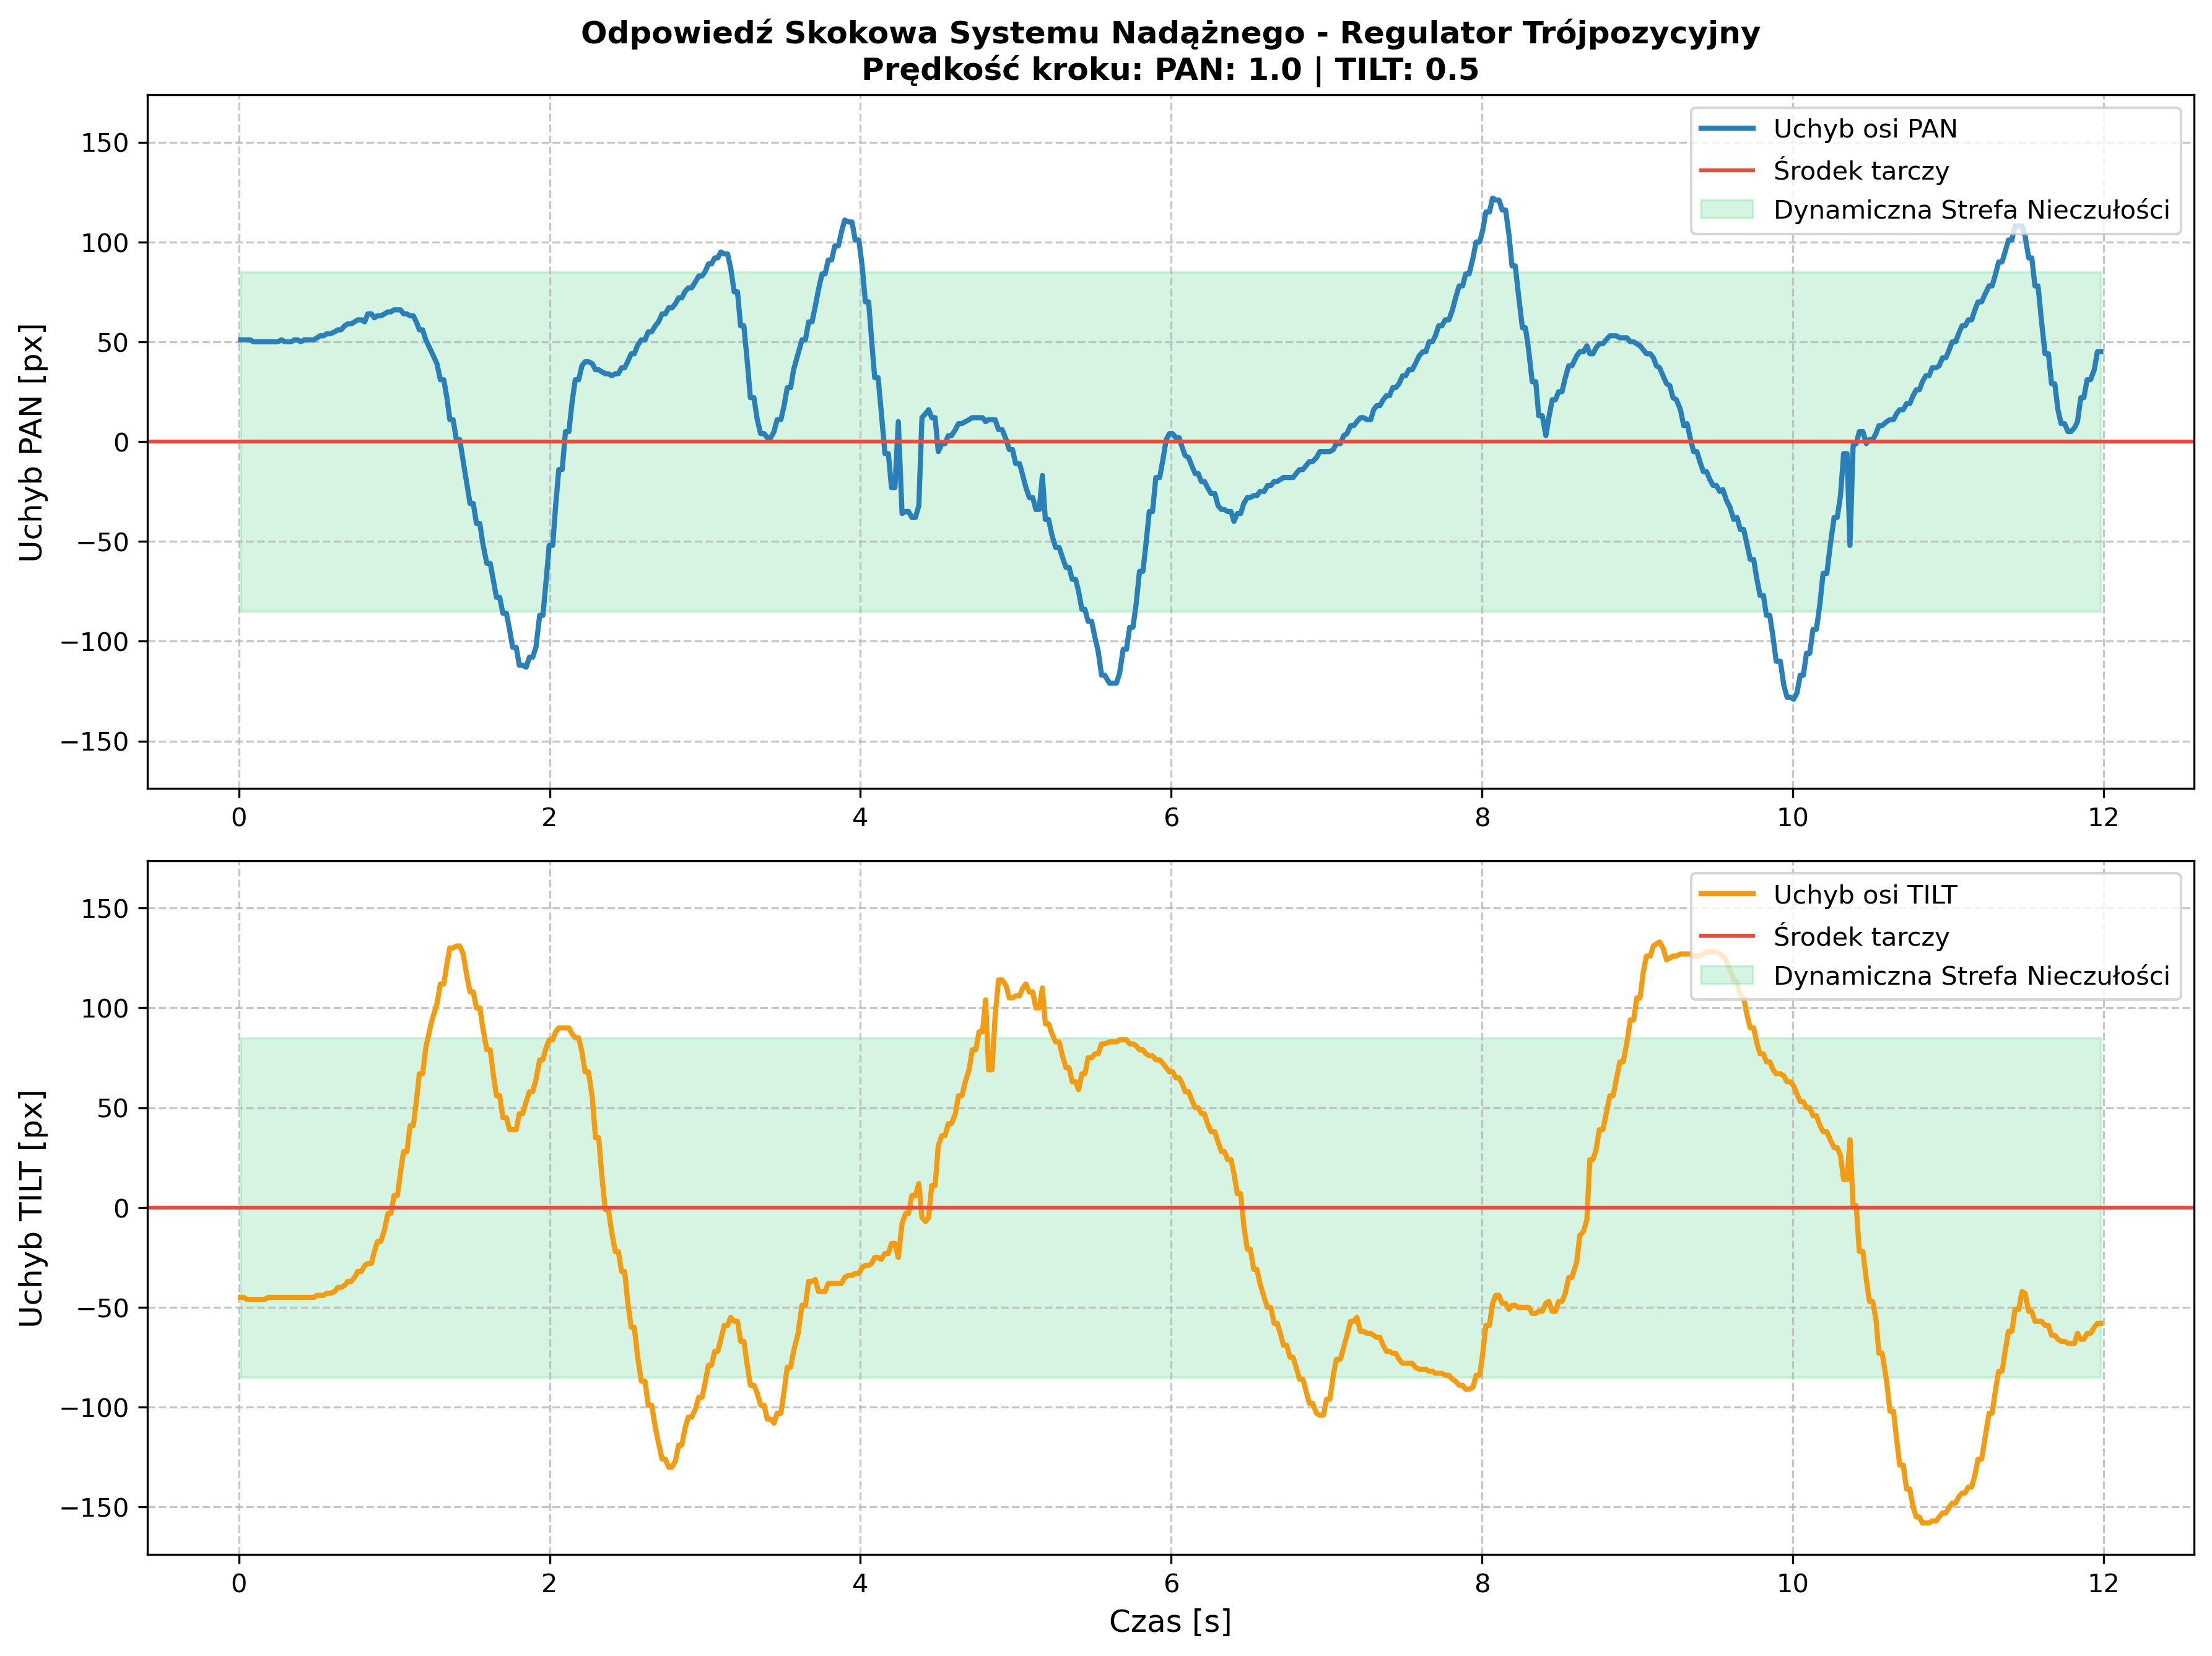
\includegraphics[width=\textwidth]{./Obrazy/WYniki troj/wykres_UP_BB_circural_150_cm.png}
    \caption{Strefa analityczna.}
\end{subfigure}
\caption{Śledzenie ruchu okrężnego dla dystansu 150~cm (Regulator trójpołożeniowy).}
\label{fig:bb_okrag_150}
\end{figure}

\subsection{Test płynnej zmiany dystansu i weryfikacja algorytmu adaptacyjnego}
\label{subsec:bb_oddalanie}

Ostatnim etapem weryfikacji algorytmu trójpołożeniowego był test odporności na nieliniową zmianę parametrów kinematycznych, zrealizowany poprzez liniowe oddalanie celu od odległości 30~cm do 150~cm wzdłuż osi optycznej obiektywu. Zmiana dystansu powoduje drastyczny spadek pozornej prędkości kątowej obiektu na matrycy oraz zmniejszenie jego pola powierzchni.

Na rys. \ref{fig:bb_oddalanie}a zaprezentowano odpowiedź układu bazowego, pracującego ze stałą, heurystyczną strefą nieczułości. W początkowej fazie eksperymentu (obiekt w bliskiej odległości), układ wygenerował permanentny cykl limitowy o potężnej amplitudzie, dochodzącej do 200 pikseli. Stan ten wynikał z faktu, że droga hamowania rozpędzonej wieżyczki wielokrotnie przekraczała założony "kaganiec". W miarę fizycznego oddalania obiektu (wraz z upływem czasu na osi odciętych), pozorna prędkość uchybu malała, co proporcjonalnie skracało drogę hamowania (nadbieg). Zjawisko to doprowadziło do naturalnego, stopniowego wygasania oscylacji, aż do momentu, gdy droga hamowania ostatecznie zmieściła się wewnątrz stałej strefy nieczułości (po 12. sekundzie).

Wdrożenie skalowanej strefy nieczułości (algorytm \textit{Gain Scheduling}) wraz z nastawami analitycznymi przyniosło radykalną poprawę jakości nadążania (rys. \ref{fig:bb_oddalanie}b). W krytycznej, początkowej fazie ruchu, system zaaplikował bezpieczną, szeroką strefę nieczułości, co skutecznie zamortyzowało dużą energię układu i całkowicie zapobiegło powstaniu początkowego cyklu limitowego. W okolicach 5. i 6. sekundy eksperymentu, gdy system wizyjny odnotował spadek pola powierzchni śledzonego konturu poniżej zaprogramowanych progów referencyjnych, algorytm skokowo redukował strefę nieczułości (widoczne zwężenie zielonego obszaru na wykresie).

\begin{figure}[!ht]
\centering
\begin{subfigure}{0.48\textwidth}
    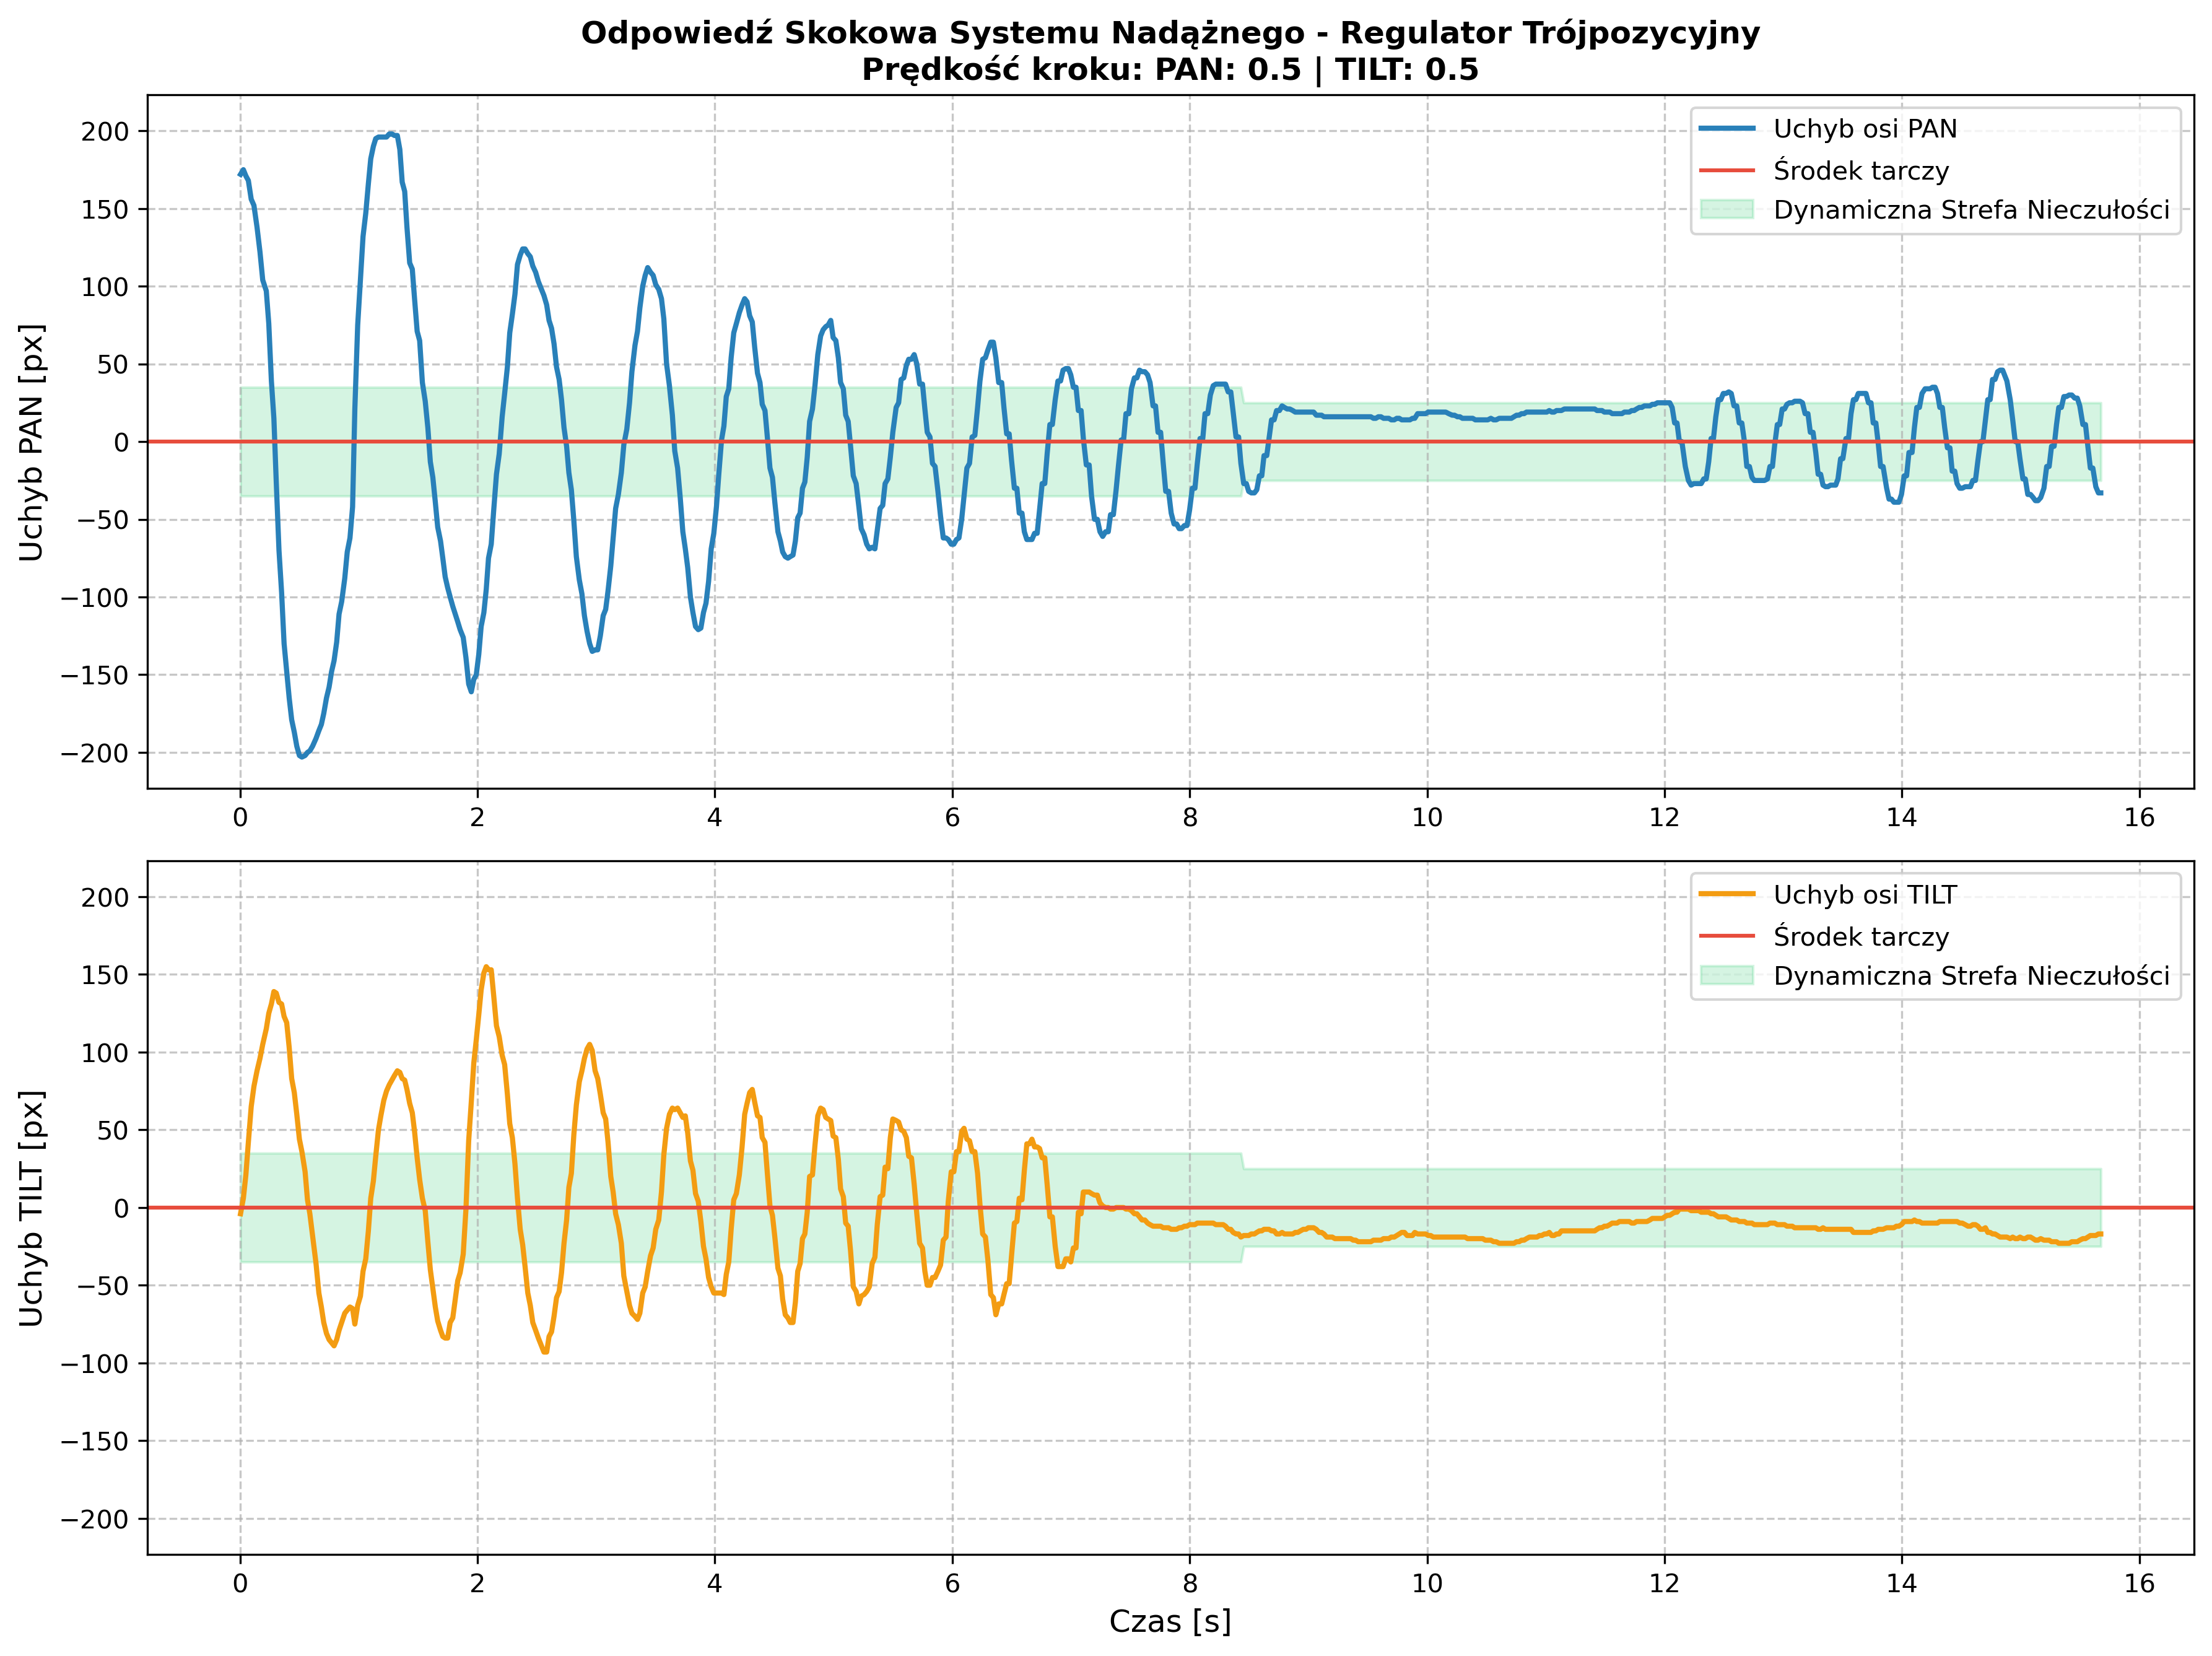
\includegraphics[width=\textwidth]{./Obrazy/WYniki troj/wykres_GOOD_BB_move_30_150.png}
    \caption{Bez adaptacji parametrów -- naturalne tłumienie drgań wraz ze wzrostem dystansu.}
\end{subfigure}
\hfill
\begin{subfigure}{0.48\textwidth}
    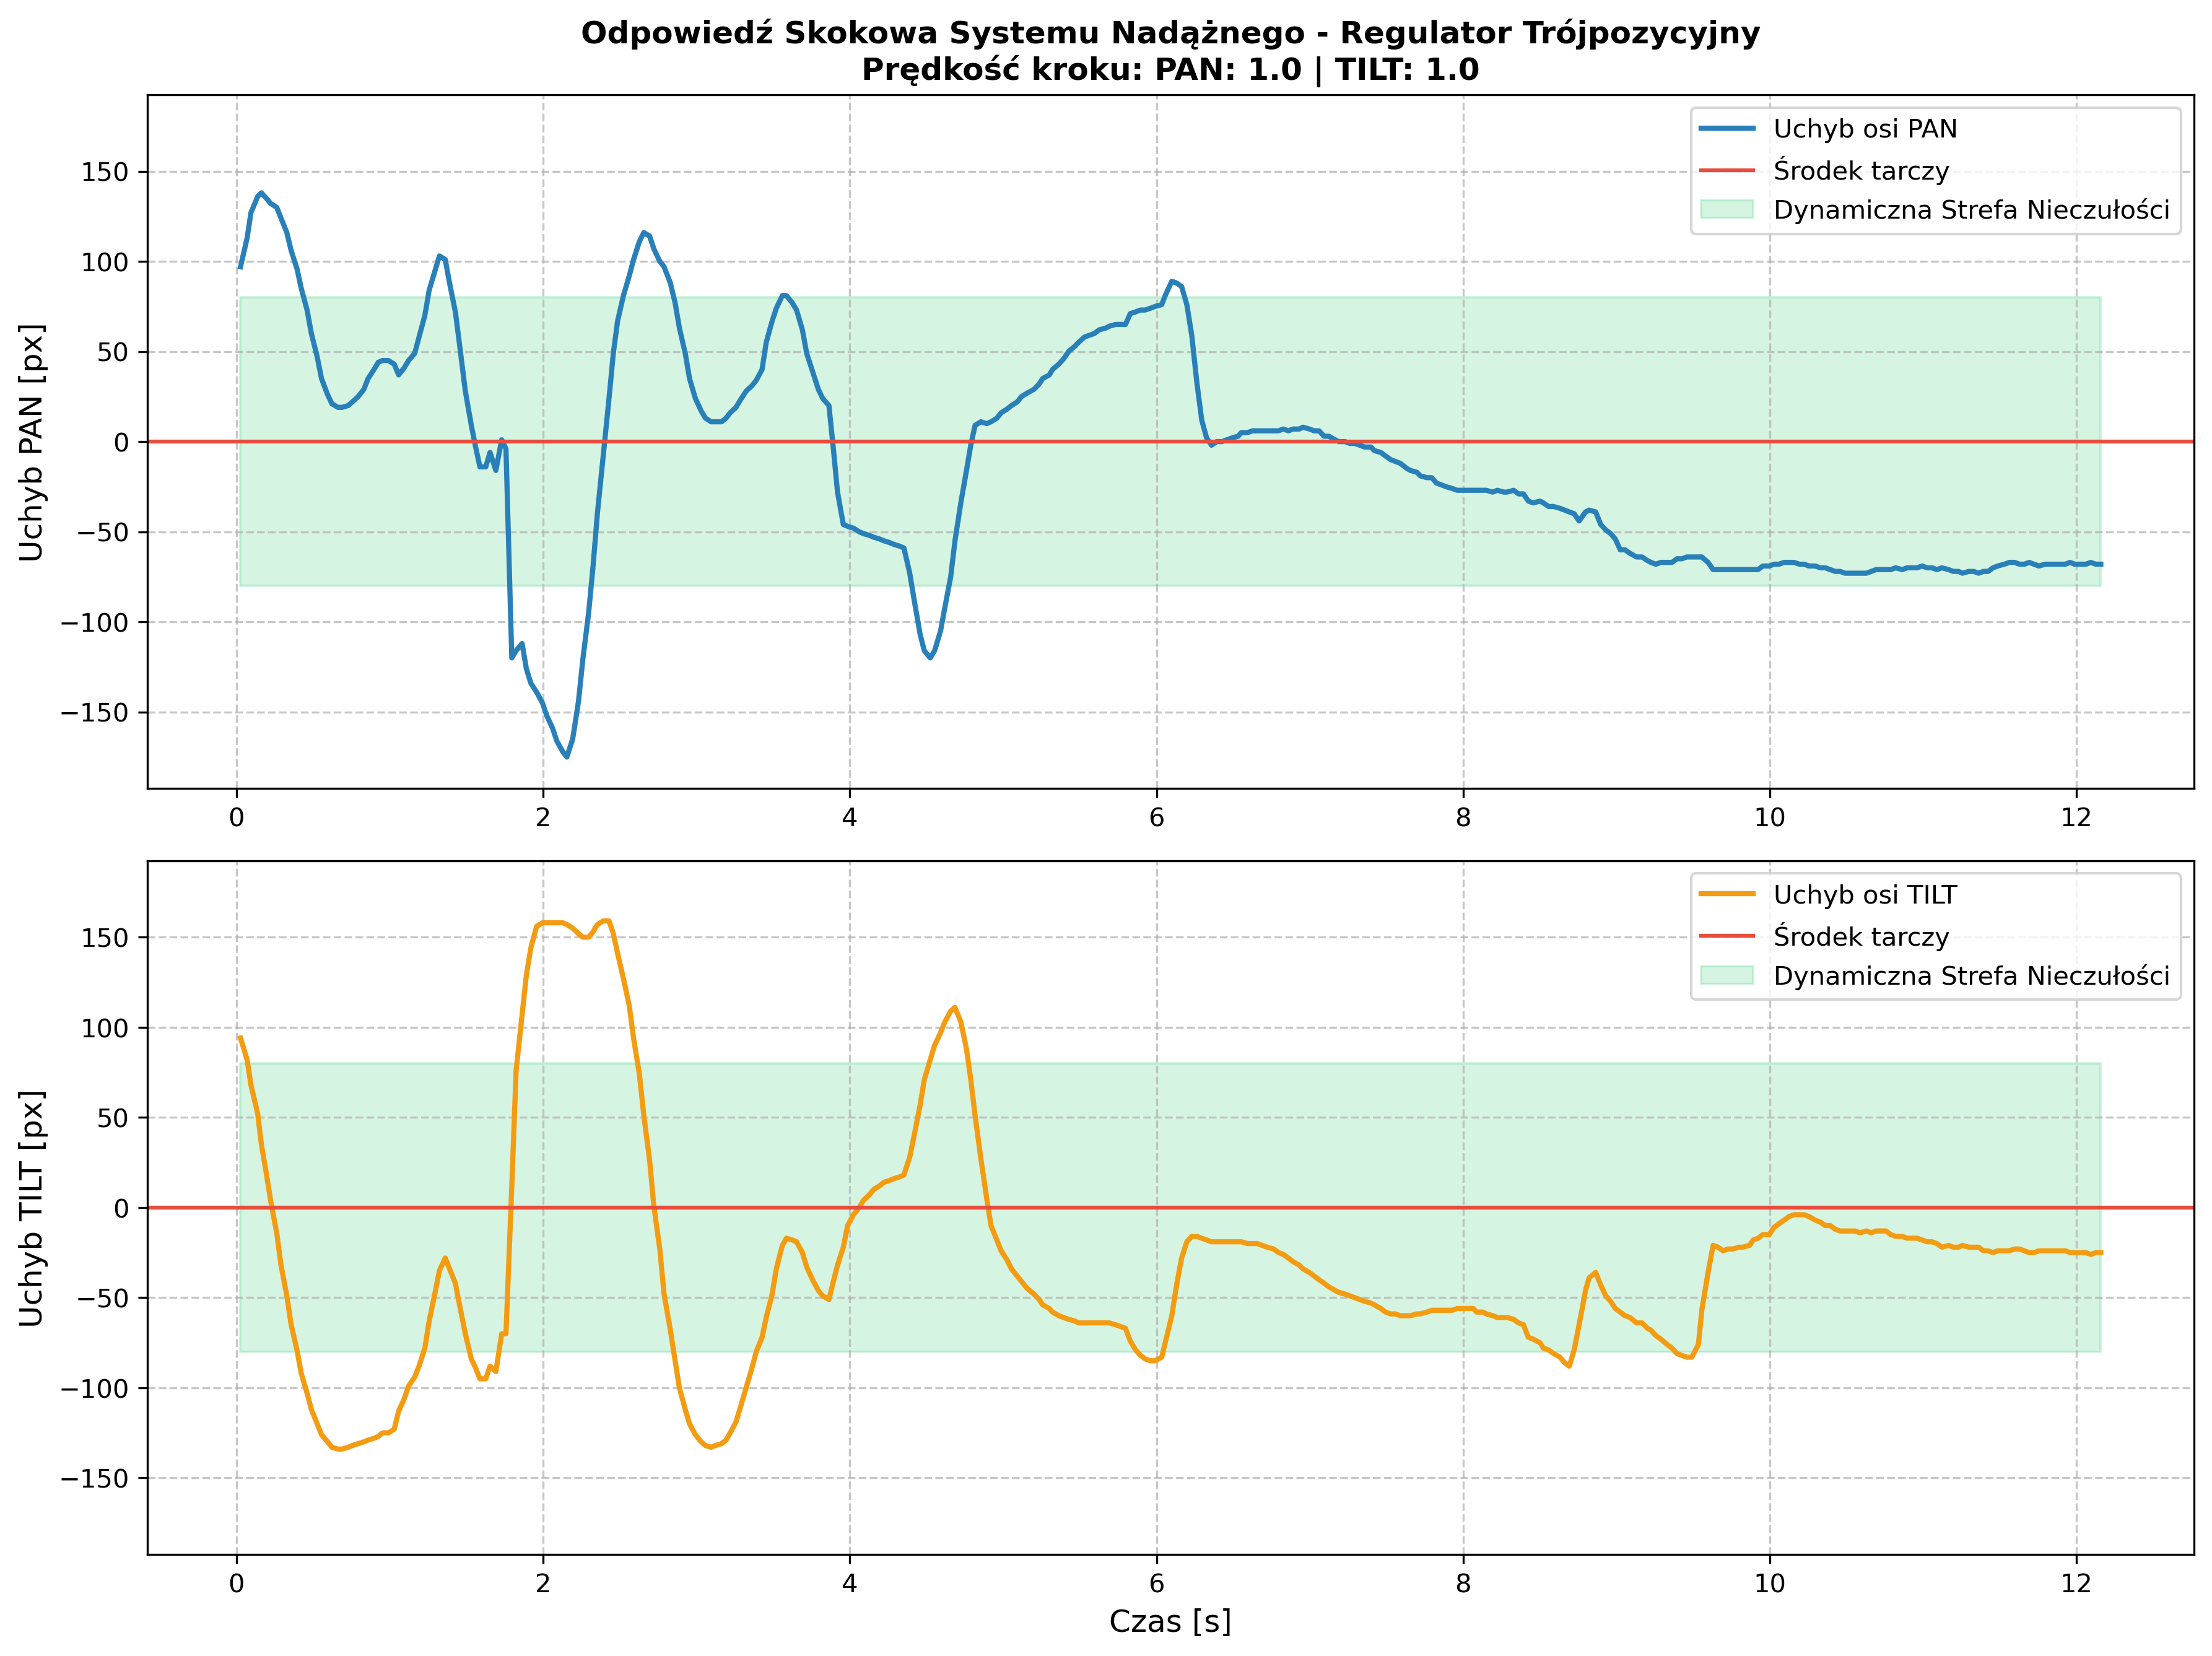
\includegraphics[width=\textwidth]{./Obrazy/WYniki troj/wykres_UP_BB_move_30_150.png}
    \caption{Aktywna adaptacja strefy -- dynamiczne zawężanie tolerancji dla oddalającego się obiektu.}
\end{subfigure}
\caption{Płynne oddalanie obiektu od 30~cm do 150~cm (Regulator trójpołożeniowy).}
\label{fig:bb_oddalanie}
\end{figure}

Dzięki takiemu rozwiązaniu regulator trójpołożeniowy zachował absolutną stabilność w bliskim kontakcie (gdzie wymagany jest szeroki margines na wyhamowanie), a jednocześnie znacząco zwiększył precyzję centrowania dla obiektów oddalonych, nie pozwalając małemu celowi na swobodne "pływanie" po matrycy.

% =========================================================
\section{Porównanie skuteczności badanych algorytmów}
\label{sec:porownanie}

\subsection{Zestawienie wskaźników jakości sterowania}
\label{subsec:wskazniki_jakosci}

W celu ostatecznej ewaluacji zaimplementowanych algorytmów, zestawiono ich zoptymalizowane odpowiedzi skokowe dla dystansu referencyjnego 80~cm. Tabela \ref{tab:porownanie_finalne} agreguje wyznaczone wskaźniki jakości regulacji.

\begin{table}[!ht]
\centering
\caption{Zestawienie wskaźników jakości regulacji dla przebadanych systemów (dystans 80~cm).}
\label{tab:porownanie_finalne}
\begin{tabular}{lccc}
\toprule
\textbf{Typ regulatora} & \textbf{Czas regulacji [s]} & \textbf{Maks. przeregulowanie [px]} & \textbf{Uchyb ustalony [px]} \\
\midrule
Bang-Bang (heurystyczne) & Niestabilny & Cykl limitowy & N/A \\
Bang-Bang (analityczne) & 0.8 & Brak & $\pm 75$ (w strefie) \\
PID (heurystyczne) & 1.5 & 120 & $\pm 10$ \\
PD (CHR + Kaganiec) & 1.1 & Brak & $\pm 25$ (w strefie) \\
\bottomrule
\end{tabular}
\end{table}

\subsection{Porównanie dynamiki w dziedzinie czasu}
\label{subsec:wykres_zbiorczy}

% Aby uwydatnić różnice w dynamice obu układów, na rys. \ref{fig:wykres_zbiorczy} nałożono na siebie przebiegi czasowe uchybu dla zoptymalizowanego algorytmu PID (metoda CHR) oraz zoptymalizowanego regulatora trójpołożeniowego.

% \begin{figure}[!ht]
% \centering
% \includegraphics[width=0.8\textwidth]{./Obrazy/Nastawy/wykres_zbiorczy_pid_vs_bb.png}
% \caption{Zbiorcze zestawienie odpowiedzi skokowych zoptymalizowanego algorytmu PID oraz regulatora trójpołożeniowego na dystansie 80~cm.}
% \label{fig:wykres_zbiorczy}
% \end{figure}

% TUTAJ OPISZEMY:
% - Szybki wjazd Bang-Bang vs powolne, miękkie lądowanie PID.

\subsection{Krzepkość układów i odporność na rozstrojenie}
\label{subsec:odpornosc_krzepkosc}
% TUTAJ OPISZEMY:
% - Wyjaśnienie, dlaczego przesterowany PID ostatecznie wygaszał drgania (dzięki Kd), a przesterowany Bang-Bang wpadał w permanentne wibracje (brak sprzężenia od pochodnej uchybu).
%\begin{itemize}
%\item prezentacja wyników, opracowanie i poszerzona dyskusja  wyników, wnioski
%\end{itemize}
%
% 
%\begin{table}
%\centering
%\caption{Opis tabeli nad nią.}
%\label{id:tab:wyniki}
%\begin{tabular}{rrrrrrrr}
%\toprule
%	         &                                     \multicolumn{7}{c}{metoda}                                      \\
%	         \cmidrule{2-8}
%	         &         &         &        \multicolumn{3}{c}{alg. 3}        & \multicolumn{2}{c}{alg. 4, $\gamma = 2$} \\
%	         \cmidrule(r){4-6}\cmidrule(r){7-8}
%	$\zeta$ &     alg. 1 &   alg. 2 & $\alpha= 1.5$ & $\alpha= 2$ & $\alpha= 3$ &   $\beta = 0.1$  &   $\beta = -0.1$ \\
%\midrule
%	       0 &  8.3250 & 1.45305 &       7.5791 &    14.8517 &    20.0028 & 1.16396 &                       1.1365 \\
%	       5 &  0.6111 & 2.27126 &       6.9952 &    13.8560 &    18.6064 & 1.18659 &                       1.1630 \\
%	      10 & 11.6126 & 2.69218 &       6.2520 &    12.5202 &    16.8278 & 1.23180 &                       1.2045 \\
%	      15 &  0.5665 & 2.95046 &       5.7753 &    11.4588 &    15.4837 & 1.25131 &                       1.2614 \\
%	      20 & 15.8728 & 3.07225 &       5.3071 &    10.3935 &    13.8738 & 1.25307 &                       1.2217 \\
%	      25 &  0.9791 & 3.19034 &       5.4575 &     9.9533 &    13.0721 & 1.27104 &                       1.2640 \\
%	      30 &  2.0228 & 3.27474 &       5.7461 &     9.7164 &    12.2637 & 1.33404 &                       1.3209 \\
%	      35 & 13.4210 & 3.36086 &       6.6735 &    10.0442 &    12.0270 & 1.35385 &                       1.3059 \\
%	      40 & 13.2226 & 3.36420 &       7.7248 &    10.4495 &    12.0379 & 1.34919 &                       1.2768 \\
%	      45 & 12.8445 & 3.47436 &       8.5539 &    10.8552 &    12.2773 & 1.42303 &                       1.4362 \\
%	      50 & 12.9245 & 3.58228 &       9.2702 &    11.2183 &    12.3990 & 1.40922 &                       1.3724 \\
%\bottomrule
%\end{tabular}
%\end{table}  
%
%
% 
%\begin{figure}
%\centering
%\begin{tikzpicture}
%\begin{axis}[
%    y tick label style={
%        /pgf/number format/.cd,
%            fixed,   % po zakomentowaniu os rzednych jest indeksowana wykladniczo
%            fixed zerofill, % 1.0 zamiast 1
%            precision=1,
%        /tikz/.cd
%    },
%    x tick label style={
%        /pgf/number format/.cd,
%            fixed,
%            fixed zerofill,
%            precision=2,
%        /tikz/.cd
%    }
%]
%\addplot [domain=0.0:0.1] {rnd};
%\end{axis} 
%\end{tikzpicture}
%\caption{Podpis rysunku po rysunkiem.}
%\label{fig:2}
%\end{figure}
%
%
%\begin{figure}
%\begin{lstlisting}
%if (_nClusters < 1)
%	throw std::string ("unknown number of clusters");
%if (_nIterations < 1 and _epsilon < 0)
%	throw std::string ("You should set a maximal number of iteration or minimal difference -- epsilon.");
%if (_nIterations > 0 and _epsilon > 0)
%	throw std::string ("Both number of iterations and minimal epsilon set -- you should set either number of iterations or minimal epsilon.");
%\end{lstlisting}
%\caption{Przykład pseudokodu}
%\end{figure}


% TODO

\chapter{Podsumowanie}

\section{Rozwiązanie problemu badawczego}
\section{Ocena osiągniętych wyników}
\section{Wnioski i rekomendacje}
\section{Perspektywy rozwoju i dalszych badań}

%\begin{itemize}
%\item Jaki problem rozwiązałæm?
%\item Jak ten problem rozwiązałæm?
%\item Jakie są dobre i słabe strony mojego rozwiązania?
%\item Czy mogę sformułować jakieś rekomendacje?
%\end{itemize}

\begin{itemize}
\item syntetyczny opis wykonanych prac
\item wnioski
\item możliwość rozwoju, kontynuacji prac, potencjalne nowe kierunki
\item Czy cel pracy zrealizowany? 
\end{itemize}



\backmatter

\cleardoublepage
\phantomsection
%\bibliographystyle{plplain}  % bibtex
%\bibliography{biblio} % bibtex
\addcontentsline{toc}{chapter}{Bibliografia}
\printbibliography           % biblatex

\begin{appendices}

% TODO
\chapter{Dokumentacja techniczna}


% TODO
\chapter{Spis skrótów i symboli}

\begin{itemize}
\item[DNA] kwas deoksyrybonukleinowy (ang. \english{deoxyribonucleic acid})
\item[MVC] model -- widok -- kontroler (ang. \english{model--view--controller}) 
\item[$N$] liczebność zbioru danych
\item[$\mu$] stopnień przyleżności do zbioru
\item[$\mathbb{E}$] zbiór krawędzi grafu
\item[$\mathcal{L}$] transformata Laplace'a 
\end{itemize}

% TODO
\chapter{Lista dodatkowych plików, uzupełniających tekst pracy (jeżeli dotyczy)} 

W systemie do pracy dołączono dodatkowe pliki zawierające:
\begin{itemize}
\item źródła programu,
\item zbiory danych użyte w~eksperymentach,
\item film pokazujący działanie opracowanego oprogramowania lub zaprojektowanego i wykonanego urządzenia,
\item itp.
\end{itemize}


\listoffigures
\addcontentsline{toc}{chapter}{Spis rysunków}
\listoftables
\addcontentsline{toc}{chapter}{Spis tabel}

\end{appendices}

\end{document}


%% Finis coronat opus.

